% ============================================================
% 《数学分析基础》主文件
% ============================================================
\documentclass[12pt,a4paper,openany]{ctexbook}

% ============================================================
% 《数学分析基础》共享导言区
% ============================================================

\usepackage{amsmath,amssymb,amsthm}
\usepackage{geometry}
\geometry{a4paper, margin=2cm, top=2.5cm, bottom=2.5cm}

\usepackage[most]{tcolorbox}
\usepackage{graphicx, array, booktabs, multirow}
\usepackage{hyperref}
\hypersetup{colorlinks=true, linkcolor=blue!60!black, urlcolor=blue!60!black}
\usepackage{fancyhdr}
\usepackage{listings}
\usepackage{xcolor}
\usepackage{enumitem}
\usepackage{fontspec}

% ── 好题标记与汇总系统 ──
\usepackage[book]{goodproblems}

% ── 中文字体 ──
\setmainfont{Times New Roman}
\setCJKmainfont{PingFang SC}

% ── 图表路径 ──
\graphicspath{{figures/}}

% ── 代码块样式 ──
\lstdefinestyle{pystyle}{
  language=Python,
  basicstyle=\small\ttfamily,
  backgroundcolor=\color{gray!5},
  frame=single,
  numbers=left,
  numberstyle=\tiny\color{gray},
  breaklines=true,
  showstringspaces=false,
  keywordstyle=\color{blue},
  commentstyle=\color{green!40!black},
  stringstyle=\color{orange!70!black},
}
\lstset{style=pystyle}

% ── 章节标题 ──
\renewcommand{\thechapter}{\arabic{chapter}}

% ── 页眉页脚 ──
\pagestyle{fancy}
\fancyhf{}
\fancyhead[LE]{\leftmark}
\fancyhead[RO]{\rightmark}
\fancyfoot[C]{\thepage}

% ============================================================
% 定理类环境（颜色编码）
% ============================================================

% 定义框（绿色）
\newtcolorbox{definitionbox}[1][]{
  colback=green!5!white, colframe=green!60!black,
  fonttitle=\bfseries, title=定义~#1
}

% 定理框（蓝色）
\newtcolorbox{theorembox}[1][]{
  colback=blue!5!white, colframe=blue!60!black,
  fonttitle=\bfseries, title=定理~#1
}

% 命题框（紫色）
\newtcolorbox{propositionbox}[1][]{
  colback=purple!5!white, colframe=purple!60!black,
  fonttitle=\bfseries, title=命题~#1
}

% 例题框（橙色）
\newtcolorbox{examplebox}[1][]{
  colback=orange!5!white, colframe=orange!70!black,
  fonttitle=\bfseries, title=例题~#1
}

% 注意框（红色）
\newtcolorbox{notebox}[1][]{
  colback=red!5!white, colframe=red!60!black,
  fonttitle=\bfseries, title=注意~#1
}

% 进步宣言框（黄色）
\newtcolorbox{progressbox}{
  colback=yellow!10!white, colframe=yellow!60!orange,
  fonttitle=\bfseries\large, title=进步宣言
}

% 应用引导框（青色）
\newtcolorbox{applicationbox}{
  colback=teal!5!white, colframe=teal!60!black,
  fonttitle=\bfseries\large, title=学完本章你能做什么？
}

% 符号卡片（灰色）
\newenvironment{symbolcard}{%
  \par\vspace{6pt}
  \noindent\begin{tcolorbox}[colback=gray!3!white, colframe=gray!50!black, arc=2pt, title=📖 符号卡片]
  \renewcommand{\arraystretch}{1.3}
  \begin{tabular}{c|c|p{3.5cm}|p{5cm}}
  \toprule
  \bfseries 符号 & \bfseries LaTeX 写法 & \bfseries 读法 & \bfseries 含义 \\
  \midrule
}{%
  \bottomrule \end{tabular} \end{tcolorbox} \par\vspace{6pt}
}

% ============================================================
% 习题环境
% ============================================================

\newcounter{exercise}[chapter]
\renewcommand{\theexercise}{\thechapter.\arabic{exercise}}

\makeatletter
\newcommand{\difficulty}[1]{%
  \ifcase#1
    \textcolor{gray}{[送]}%
  \or
    \textcolor{gray}{[简]}%
  \or
    \textcolor{green!40!black}{[基]}%
  \or
    \textcolor{blue}{[普]}%
  \or
    \textcolor{orange}{[中]}%
  \or
    \textcolor{red}{[进]}%
  \or
    \textcolor{purple}{[拔]}%
  \or
    \textcolor{red!70!black}{[极]}%
  \or
    \textcolor{red!90!black}{[竞]}%
  \fi
}
\makeatother

\newenvironment{exercise}[1][0]{% 参数：难度等级 0-9
  \refstepcounter{exercise}
  \par\vspace{8pt}
  \noindent
  \textbf{练习 \theexercise}~\difficulty{#1}\quad
  \ignorespaces
}{\par\vspace{4pt}}

% 答案环境（放附录）
\newenvironment{answer}[1]{% 参数：练习编号
  \par\vspace{6pt}
  \noindent\textbf{#1}\quad
  \ignorespaces
}{\par\vspace{4pt}}

% ── 好题标记（最简单的用法）──
% 在 exercise 里面写 \好题 就行，不用起名字
\makeatletter
\newcommand{\好题}{%
  \edef\@gp@label{ex:\thechapter-\arabic{exercise}}%
  \label{prob:\@gp@label}%
  \GP@write{\string\GPentry{\theexercise}{\@gp@label}}%
}
\newcommand{\好答}{%
  \edef\@gp@label{ex:\thechapter-\arabic{exercise}}%
  \label{sol:\@gp@label}%
}
\makeatother

% ============================================================
% 其他设置
% ============================================================

% 图片不浮动（保持位置）
\setcounter{topnumber}{5}
\setcounter{bottomnumber}{5}
\setcounter{totalnumber}{10}

% 列表紧凑
\setlist{nosep}



% ── 自学教学设计环境 ──
\newtcolorbox{hintref}{colback=gray!5!white, colframe=gray!40!black,
  arc=2pt, left=4pt, right=4pt, top=3pt, bottom=3pt,
  fonttitle=\small\bfseries, title=提示}
\newtcolorbox{confidencebox}{colback=white, colframe=purple!40!black,
  arc=2pt, left=6pt, right=6pt, top=4pt, bottom=4pt,
  fonttitle=\small\bfseries, title=信心校准}
\newtcolorbox{retrievalgatebox}{colback=white, colframe=orange!60!black,
  arc=2pt, left=6pt, right=6pt, top=4pt, bottom=4pt,
  fonttitle=\small\bfseries, title=先想后看}


\title{\Huge 数学分析基础}
\author{\large 从函数重建到严格分析}
\date{\large 共六编三十章}

\begin{document}

\maketitle
\tableofcontents
\newpage

% ============================================================
% 第〇编：函数基础重建
% ============================================================
\part{函数基础重建——从对应关系到六类基本函数}
% ============================================================
% 第1章：函数的概念——从输入输出到对应法则
% ============================================================

\chapter{函数的概念——从输入输出到对应法则}

\begin{applicationbox}
\textbf{学完本章你能做什么？}
\begin{enumerate}
  \item \textbf{学之前}：你会解方程，知道"x 等于多少"——但只能得到\textbf{一个数}。
  \item \textbf{学之后}：你能描述"当 x 变化时，y 跟着怎么变"——从一个数扩展到\textbf{一整条线}。
  \item \textbf{日常例子}：你打车，起步价 10 元，每公里 2 元。行驶里程不同，车费就不同。
        如果里程是变量，车费就是\textbf{里程的函数}——输入一个里程，输出对应的车费。
\end{enumerate}
\end{applicationbox}


% ============================================================
\section{从方程到函数——为什么需要函数？}
% ============================================================

你已经会解方程了。比如：

\[
2x + 1 = 7
\]

解出来：\(x = 3\)。好，得到了一个数，问题结束。

但现实世界不是这样的。现实中的问题通常是：

\begin{center}
\fcolorbox{blue!40}{blue!5}{\parbox{0.85\textwidth}{
\textbf{问题：}出租车车费 = 起步价 10 元 + 每公里 2 元。\\
你坐了多少公里？车费是多少？\textbf{——这取决于你坐了多远。}}}
\end{center}

你看，这里的车费\textbf{不是固定的一个数}，而是随着里程的变化而变化。\\
如果里程是 \(x\) 公里，车费就是 \(10 + 2x\) 元。

\begin{itemize}
  \item \(x = 0\) 公里 \(\rightarrow\) 车费 = \(10 + 2\times 0 = 10\) 元
  \item \(x = 3\) 公里 \(\rightarrow\) 车费 = \(10 + 2\times 3 = 16\) 元
  \item \(x = 10\) 公里 \(\rightarrow\) 车费 = \(10 + 2\times 10 = 30\) 元
  \item \(x = 15\) 公里 \(\rightarrow\) 车费 = \(10 + 2\times 15 = 40\) 元
\end{itemize}

\textbf{不同输入，产生不同输出}——这就是函数的核心思想。

\begin{notebox}
方程和函数的关键区别：
\begin{itemize}
  \item \textbf{方程}：\(2x + 1 = 7\)——你找的是\textbf{一个特定的数}让等式成立。
  \item \textbf{函数}：\(y = 2x + 1\)——你问的是\textbf{当 x 变化时，y 怎么跟着变}。
\end{itemize}
用一句话说：\textbf{方程是找点，函数是看线。}
\end{notebox}


% ============================================================
\section{函数的定义——什么是函数？}
% ============================================================

\subsection{从具体例子出发}

先看三个例子：

\begin{examplebox}[1]
小明和小红在数轴上玩一个游戏：小明说出一个数，小红用规则算出另一个数。

\begin{center}
\begin{tabular}{c|c}
\textbf{小明说的数（输入）} & \textbf{小红算出的数（输出）} \\
\hline
1 & 3 \\
2 & 5 \\
3 & 7 \\
4 & 9 \\
5 & 11 \\
\end{tabular}
\end{center}

你能发现规律吗？\\
小红每次都是把小明说的数 \textbf{乘以 2 再加 1}。\\
如果小明说的数是 \(x\)，小红算出的数就是 \(2x + 1\)。
\end{examplebox}

\begin{examplebox}[2]
一个正方形的边长变化时，面积怎么变？

\begin{center}
\begin{tabular}{c|c}
\textbf{边长（cm）} & \textbf{面积（cm\(^2\)）} \\
\hline
1 & \(1\times1 = 1\) \\
2 & \(2\times2 = 4\) \\
3 & \(3\times3 = 9\) \\
4 & \(4\times4 = 16\) \\
\end{tabular}
\end{center}

规律：面积 = 边长 \(\times\) 边长。\\
边长用 \(x\) 表示，面积就是 \(x^2\)。
\end{examplebox}

\begin{examplebox}[3]
一杯热水在冷却，温度随时间变化（每分钟测一次）：

\begin{center}
\begin{tabular}{c|c}
\textbf{时间（分钟）} & \textbf{温度（℃）} \\
\hline
0 & 80 \\
1 & 72 \\
2 & 65 \\
3 & 59 \\
4 & 54 \\
\end{tabular}
\end{center}

温度随着时间增长而下降——这也是一个函数关系。
\end{examplebox}

这三个例子有一个共同特点：

\begin{quote}
\textbf{有一个输入，按照一个规则，得到一个输出。每个输入对应唯一的输出。}
\end{quote}

\subsection{函数的正式定义}

\begin{definitionbox}[函数的概念]
设 \(D\) 是一个非空数集。如果存在一个对应法则 \(f\)，使得对 \(D\) 中的\textbf{每一个}数 \(x\)，
按照 \(f\) 都能\textbf{唯一确定}一个实数 \(y\)，那么称 \(f\) 是定义在 \(D\) 上的一个\textbf{函数}。

记作：
\[
f: D \to \mathbb{R}, \qquad x \mapsto y
\]

其中：
\begin{itemize}
  \item \(x\) 叫\textbf{自变量}（读作 zì biàn liàng，英文 independent variable）
  \item \(y\) 叫\textbf{因变量}（读作 yīn biàn liàng，英文 dependent variable）
  \item \(D\) 叫\textbf{定义域}（读作 dìng yì yù，英文 domain）
  \item 全体输出值组成的集合叫\textbf{值域}（读作 zhí yù，英文 range）
  \item \(y\) 也记作 \(f(x)\)，读作"f of x"
\end{itemize}
\end{definitionbox}

\begin{notebox}
函数的三个要素缺一不可：
\[
\boxed{\mbox{定义域} \;+\; \mbox{对应法则} \;+\; \mbox{值域}}
\]

其中对应法则是\textbf{核心}，定义域是\textbf{前提}，值域是\textbf{结果}。
\end{notebox}

\subsection{用"黑箱"理解函数}

想象一个黑箱：

\begin{center}
\fbox{
\parbox{0.7\textwidth}{
\[
\xrightarrow{\;x\;}\;
\fcolorbox{blue!30}{blue!10}{\parbox{0.3\textwidth}{\centering \textbf{函数 \(f\)}\\\small 输入 \(\to\) 规则 \(\to\) 输出}}
\;\xrightarrow{\;f(x)\;}
\]
}}
\end{center}

你从左边放进一个 \(x\)，黑箱按照规则 \(f\) 处理，右边出来一个 \(f(x)\)。

\begin{itemize}
  \item 放进去 \(x=1\)，出来 \(f(1)\)
  \item 放进去 \(x=2\)，出来 \(f(2)\)
  \item 放进去 \(x=100\)，出来 \(f(100)\)
\end{itemize}

\textbf{每个输入只能出来一个输出}——这是函数最根本的规则。\\
如果一个输入对应两个输出，那就不是函数。

\begin{examplebox}[4]
判断下面哪些是函数（用定义检验）：

(1) \(y = 3x - 2\)，\(x \in \mathbb{R}\)

解：对每个 \(x\)，\(3x - 2\) 唯一确定。\(\rightarrow\) \textbf{是函数}。

(2) \(y^2 = x\)，\(x \ge 0\)

解：当 \(x = 4\) 时，\(y^2 = 4\)，\(y = 2\) 或 \(y = -2\)。一个输入对应两个输出。\(\rightarrow\) \textbf{不是函数}。

(3) 每个学生的身高

解：输入是"学生"，输出是"身高（cm）"。每个学生只有一个身高。\(\rightarrow\) \textbf{是函数}。
\end{examplebox}


% ============================================================
\section{函数的表示法}
% ============================================================

函数有三种常见的表示方式：

\begin{definitionbox}[函数的三种表示法]
\begin{enumerate}
  \item \textbf{解析法}：用数学公式表示。例如 \(f(x) = x^2 + 1\)。
  \item \textbf{列表法}：用表格列出输入和输出的对应值。
  \item \textbf{图像法}：在坐标系中画出所有点 \((x, f(x))\)。
\end{enumerate}
三种方式各有优缺点，通常我们会结合使用。
\end{definitionbox}

\subsection{解析法——最精确}

用公式表达对应法则，是最常用的方法。

\begin{examplebox}[5]
已知 \(f(x) = 2x^2 - 3x + 1\)，求 \(f(0)\)、\(f(1)\)、\(f(-2)\)、\(f(a)\)。

解：
\[
\begin{aligned}
f(0) &= 2 \times 0^2 - 3 \times 0 + 1 \\
     &= 0 - 0 + 1 \\
     &= 1
\end{aligned}
\]

\[
\begin{aligned}
f(1) &= 2 \times 1^2 - 3 \times 1 + 1 \\
     &= 2 \times 1 - 3 + 1 \\
     &= 2 - 3 + 1 \\
     &= 0
\end{aligned}
\]

\[
\begin{aligned}
f(-2) &= 2 \times (-2)^2 - 3 \times (-2) + 1 \\
      &= 2 \times 4 - (-6) + 1 \\
      &= 8 + 6 + 1 \\
      &= 15
\end{aligned}
\]

\[
\begin{aligned}
f(a) &= 2 \times a^2 - 3 \times a + 1 \\
     &= 2a^2 - 3a + 1
\end{aligned}
\]

\textbf{重要：} \(f(a)\) 不是"f 乘以 a"，而是"把 \(a\) 代入函数 \(f\) 后得到的结果"。
\end{examplebox}

\subsection{列表法——最直观}

把输入和输出列成表格，一目了然。

\begin{examplebox}[6]
一天中每个整点的气温：

\begin{center}
\begin{tabular}{c|c}
\textbf{时间（时）} & \textbf{气温（℃）} \\
\hline
6 & 18 \\
8 & 21 \\
10 & 25 \\
12 & 28 \\
14 & 29 \\
16 & 27 \\
18 & 24 \\
20 & 21 \\
\end{tabular}
\end{center}

这就是用\textbf{列表法}表示的函数。
\end{examplebox}

\subsection{图像法——最形象}

在平面直角坐标系中，把所有点 \((x, f(x))\) 画出来，就得到了函数的图像。

\begin{examplebox}[7]
画出 \(f(x) = x^2\) 的图像：

先列表：
\begin{center}
\begin{tabular}{c|c|c|c|c|c|c|c}
\(x\) & -3 & -2 & -1 & 0 & 1 & 2 & 3 \\
\hline
\(f(x) = x^2\) & 9 & 4 & 1 & 0 & 1 & 4 & 9 \\
\end{tabular}
\end{center}

把这些点 \((-3,9), (-2,4), (-1,1), (0,0), (1,1), (2,4), (3,9)\) 画在坐标系中，
然后用平滑曲线连接——就得到了一个开口向上的抛物线。
\end{examplebox}

\begin{theorembox}[垂线检验法]
如何判断一条曲线是不是函数的图像？

\textbf{方法}：在图像上任意画一条竖直线（与 \(y\) 轴平行的线）。
\begin{itemize}
  \item 如果每条竖直线\textbf{最多只与图像交于一个点}，那么它是函数的图像。
  \item 如果某条竖直线与图像交于两个或更多点，那么它不是函数的图像。
\end{itemize}

\textbf{原因}：一个 \(x\) 只能对应一个 \(y\)。如果一条竖直线 \(x = a\) 与图像有两个交点，
意味着 \(x = a\) 对应两个不同的 \(y\) 值，违背了函数的定义。
\end{theorembox}


% ============================================================
\section{定义域的求法——哪些 \(x\) 是允许的？}
% ============================================================

定义域是函数\textbf{所有允许的输入值}组成的集合。\\
不是所有的数都能代入一个函数——有些输入会导致无意义的结果。

\subsection{常见的限制条件}

\begin{definitionbox}[定义域的常见限制]
\begin{enumerate}
  \item \textbf{分母不能为 0}：如果函数有分母，分母 \(\neq 0\)。
  \item \textbf{偶次根号下非负}：\(\sqrt{\,\cdot\,}\) 里面必须 \(\ge 0\)。
  \item \textbf{对数真数大于 0}：\(\ln(\,\cdot\,)\) 里面必须 \(> 0\)（以后学）。
\end{enumerate}
\end{definitionbox}

\subsection{求定义域的例题}

\begin{examplebox}[8]
求 \(f(x) = \dfrac{1}{x - 3}\) 的定义域。

解：
\[
\mbox{分母不能为 0} \;\Longrightarrow\; x - 3 \neq 0 \;\Longrightarrow\; x \neq 3
\]

用区间表示：
\[
(-\infty, 3) \cup (3, +\infty)
\]

读作："负无穷到 3，并上 3 到正无穷"。
\end{examplebox}

\begin{examplebox}[9]
求 \(f(x) = \sqrt{5 - x}\) 的定义域。

解：
\[
\mbox{根号下非负} \;\Longrightarrow\; 5 - x \ge 0 \;\Longrightarrow\; -x \ge -5 \;\Longrightarrow\; x \le 5
\]

用区间表示：\((-\infty, 5]\)。

\textbf{注意：} \(x = 5\) 是允许的，因为 \(\sqrt{0} = 0\) 有意义，所以用\textbf{闭区间}。
\end{examplebox}

\begin{examplebox}[10]
求 \(f(x) = \dfrac{1}{\sqrt{x + 2}}\) 的定义域。

解：这里既有分母又有根号，需要\textbf{同时满足}两个条件：
\[
\begin{cases}
\mbox{分母} \neq 0：& \sqrt{x + 2} \neq 0 \\
\mbox{根号下} \ge 0：& x + 2 \ge 0
\end{cases}
\]

由 \(\sqrt{x + 2} \neq 0\) 得：\(x + 2 \neq 0\)，即 \(x \neq -2\)。\\
由 \(x + 2 \ge 0\) 得：\(x \ge -2\)。

同时成立：\(x \ge -2\) 且 \(x \neq -2\)，即 \(x > -2\)。

用区间表示：\((-2, +\infty)\)。

\textbf{验证：}
\begin{itemize}
  \item \(x = -1\)：\(\dfrac{1}{\sqrt{-1 + 2}} = \dfrac{1}{\sqrt{1}} = 1\)，有意义 [OK]
  \item \(x = -2\)：\(\dfrac{1}{\sqrt{-2 + 2}} = \dfrac{1}{0}\)，分母为 0，无意义 [X]
  \item \(x = -3\)：\(\sqrt{-3 + 2} = \sqrt{-1}\)，负数开方，无意义 [X]
\end{itemize}
\end{examplebox}

\begin{examplebox}[11]
求 \(f(x) = \dfrac{1}{x^2 - 4}\) 的定义域。

解：
\[
x^2 - 4 \neq 0 \;\Longrightarrow\; (x - 2)(x + 2) \neq 0 \;\Longrightarrow\; x \neq 2 \mbox{ 且 } x \neq -2
\]

用区间表示：
\[
(-\infty, -2) \cup (-2, 2) \cup (2, +\infty)
\]

画出数轴：
\begin{center}
\fbox{\parbox{0.6\textwidth}{
\(-\infty\) \(\xrightarrow{\qquad}\) \(-2\) \(\xrightarrow{\qquad}\) \(2\) \(\xrightarrow{\qquad}\) \(+\infty\)\\
\hspace*{1cm} \(-2\) 和 \(2\) 这两个点被挖掉了
}}
\end{center}
\end{examplebox}

\begin{examplebox}[12]
求 \(f(x) = \sqrt{4 - x} + \dfrac{1}{x - 1}\) 的定义域。

解：两个部分\textbf{同时要有意义}：
\[
\begin{cases}
4 - x \ge 0 \;\Longrightarrow\; x \le 4 \\
x - 1 \neq 0 \;\Longrightarrow\; x \neq 1
\end{cases}
\]

所以定义域是 \((-\infty, 1) \cup (1, 4]\)。

\textbf{验证：}
\begin{itemize}
  \item \(x = 0\)：\(\sqrt{4 - 0} + \dfrac{1}{0 - 1} = 2 - 1 = 1\) [OK]
  \item \(x = 1\)：分母为 0 [X]
  \item \(x = 4\)：\(\sqrt{4 - 4} + \dfrac{1}{4 - 1} = 0 + \dfrac{1}{3} = \dfrac{1}{3}\) [OK]
  \item \(x = 5\)：\(\sqrt{4 - 5} = \sqrt{-1}\) [X]
\end{itemize}
\end{examplebox}


% ============================================================
\section{分段函数——不同区间，不同规则}
% ============================================================

有些函数在不同的输入范围内使用\textbf{不同的对应法则}——这叫分段函数。

\begin{definitionbox}[分段函数]
分段函数是指在不同区间上用不同表达式定义的函数。

\[
f(x) =
\left\{
\begin{array}{ll}
\text{表达式一}, & x \text{ 在范围一内} \\
\text{表达式二}, & x \text{ 在范围二内} \\
\ldots
\end{array}
\right.
\]
\end{definitionbox}

\begin{examplebox}[13]
已知：
\[
f(x) =
\begin{cases}
x + 1, & x \ge 0 \\
x^2,   & x < 0
\end{cases}
\]

求 \(f(2)\)、\(f(-1)\)、\(f(0)\)。

解：
\begin{itemize}
  \item \(f(2)\)：因为 \(2 \ge 0\)，代入 \(x + 1\)：\(2 + 1 = 3\)
  \item \(f(-1)\)：因为 \(-1 < 0\)，代入 \(x^2\)：\((-1)^2 = 1\)
  \item \(f(0)\)：因为 \(0 \ge 0\)（包含等号），代入 \(x + 1\)：\(0 + 1 = 1\)
\end{itemize}

\textbf{关键：} 先看 \(x\) 落在哪个区间，再代入对应的表达式。
\end{examplebox}

\begin{examplebox}[14——实际应用：阶梯电价]
某城市的电费收费标准：
\begin{itemize}
  \item 每月用电量不超过 100 度，每度 0.5 元
  \item 超过 100 度但不超过 300 度的部分，每度 0.7 元
  \item 超过 300 度的部分，每度 1.0 元
\end{itemize}

用电量 \(x\)（度）和电费 \(f(x)\)（元）的关系：

\[
f(x) =
\begin{cases}
0.5x,                 & 0 \le x \le 100 \\
50 + 0.7(x - 100),    & 100 < x \le 300 \\
50 + 140 + 1.0(x - 300), & 300 < x
\end{cases}
\]

计算：
\begin{itemize}
  \item 用电 80 度：\(0.5 \times 80 = 40\) 元
  \item 用电 200 度：\(50 + 0.7 \times (200 - 100) = 50 + 70 = 120\) 元
  \item 用电 400 度：\(50 + 140 + 1.0 \times (400 - 300) = 50 + 140 + 100 = 290\) 元
\end{itemize}

\textbf{这就是分段函数在生活中的一个典型应用。}
\end{examplebox}


% ============================================================
\section{函数与方程的联系}
% ============================================================

函数和方程不是两件不相干的事——它们是\textbf{同一个硬币的两面}。

\begin{examplebox}[15]
看函数 \(y = 2x + 1\)。

\begin{itemize}
  \item 在函数视角中：当 \(x = 1\) 时，\(y = 3\)；当 \(x = 2\) 时，\(y = 5\)……
  \item 在方程视角中：如果问"什么时候 \(y = 7\)？"——就是解方程 \(2x + 1 = 7\)，得 \(x = 3\)。
\end{itemize}

\textbf{方程的解 = 函数取特定值时对应的自变量值。}

用图像来看：方程 \(2x + 1 = 7\) 的解，就是直线 \(y = 2x + 1\) 与水平线 \(y = 7\) 的交点的 \(x\) 坐标。
\end{examplebox}


% ============================================================
\section{符号卡片}
% ============================================================

\begin{symbolcard}
\(f\) & \verb|f| & 读作"f" & 表示一个函数的名字 \\
\(f(x)\) & \verb|f(x)| & 读作"f of x" & 函数 \(f\) 在 \(x\) 处的值 \\
\(f: D \to \mathbb{R}\) & \verb|f: D \to \mathbb{R}| & 读作"从 D 到实数集的映射" & \(f\) 的定义域是 \(D\)，值在实数中 \\
\(x\) & \verb|x| & 读作"艾克斯" & 自变量，即输入 \\
\(y\) & \verb|y| & 读作"歪" & 因变量，即输出 \\
\(\mathbb{R}\) & \verb|\mathbb{R}| & 读作"实数集" & 全体实数的集合 \\
\((-\infty, +\infty)\) & \verb|(-\infty, +\infty)| & 读作"负无穷到正无穷" & 全体实数 \\
\(\cup\) & \verb|\cup| & 读作"并" & 集合的并运算 \\
\end{symbolcard}


% ============================================================
\section{代码验证}
% ============================================================

\begin{lstlisting}[caption=用 Python 理解函数的概念]
# 函数就是"输入$\to$规则$\to$输出"
# 在 Python 中，函数也是用 def 定义的

# 例1：出租车车费函数
def car_fare(km):
    """车费 = 起步价 10 + 每公里 2 元"""
    return 10 + 2 * km

print("=== 出租车函数 ===")
for d in [0, 3, 10, 15]:
    print(f"  行驶 {d:2d} 公里 $\to$ 车费 {car_fare(d):2d} 元")

print()

# 例2：f(x) = 2x^2 - 3x + 1
def f(x):
    return 2*x**2 - 3*x + 1

print("=== f(x) = 2x² - 3x + 1 ===")
for val in [0, 1, -2, 5]:
    print(f"  f({val:3d}) = {f(val)}")

print()

# 例3：分段函数 f(x) = x+1 (x>=0), x² (x<0)
def piecewise(x):
    if x >= 0:
        return x + 1
    else:
        return x**2

print("=== 分段函数 ===")
for val in [2, -1, 0, -3, 5]:
    print(f"  f({val:3d}) = {piecewise(val)}")

print()

# 例4：求定义域（数值验证——代入测试）
def test_domain(f, test_values):
    """测试一些值是否在定义域内"""
    for x in test_values:
        try:
            result = f(x)
            print(f"  x = {x:4.1f} $\to$ f(x) = {result:.4f}  [OK]")
        except (ZeroDivisionError, ValueError):
            print(f"  x = {x:4.1f} -> 无定义 [X]")

print("=== 测试 f(x) = 1/sqrt(x+2) 的定义域 ===")
def g(x):
    return 1 / (x + 2)**0.5

test_domain(g, [-3, -2.5, -2, -1.5, -1, 0, 2, 5])
\end{lstlisting}

运行结果：
\begin{lstlisting}[frame=none,backgroundcolor={},numbers=none]
=== 出租车函数 ===
  行驶  0 公里 -> 车费 10 元
  行驶  3 公里 -> 车费 16 元
  行驶 10 公里 -> 车费 30 元
  行驶 15 公里 -> 车费 40 元

=== f(x) = 2x^2 - 3x + 1 ===
  f(  0) = 1
  f(  1) = 0
  f( -2) = 15
  f(  5) = 36

=== 分段函数 ===
  f(  2) = 3
  f( -1) = 1
  f(  0) = 1
  f( -3) = 9
  f(  5) = 6

=== 测试 f(x) = 1/sqrt(x+2) 的定义域 ===
  x = -3.0 -> 无定义 [X]
  x = -2.5 -> 无定义 [X]
  x = -2.0 -> 无定义 [X]
  x = -1.5 -> f(x) = 1.4142  [OK]
  x = -1.0 -> f(x) = 1.0000  [OK]
  x =  0.0 -> f(x) = 0.7071  [OK]
  x =  2.0 -> f(x) = 0.5000  [OK]
  x =  5.0 -> f(x) = 0.3780  [OK]
\end{lstlisting}


% ============================================================
\section{本章小结}
% ============================================================

\begin{progressbox}
函数的三要素：\textbf{定义域}（输入范围）+ \textbf{对应法则}（规则）+ \textbf{值域}（输出范围）

三种表示法：\textbf{解析法}（公式）、\textbf{列表法}（表格）、\textbf{图像法}（图像）

定义域的限制：分母 \(\neq 0\)、偶次根号下 \(\ge 0\)

分段函数：不同区间用不同规则

函数与方程的关系：方程的解是函数取特定值时的自变量值
\end{progressbox}

\subsection*{通往下一章}

\textbf{这一章}你学会了什么是函数——输入经过规则产生唯一输出。

\textbf{下一章}我们将学习\textbf{函数的图像}——把抽象的对应关系变成直观的图形。
你会看到：一个函数长什么样？怎么从图像看出函数的性质？
图像是连接代数与几何的第一座桥梁。


% ============================================================
% 习题
% ============================================================
\section{习题}

% ===== 送分 =====

\begin{exercise}[0]
判断以下哪些是函数（回答"是"或"不是"）：
\begin{enumerate}
  \item[(1)] 每个学生的学号对应一个姓名
  \item[(2)] \(y = \pm \sqrt{x}\)（\(x \ge 0\)）
  \item[(3)] 每个时间点对应当时的室内温度
\end{enumerate}
\end{exercise}

\begin{exercise}[0]
已知 \(f(x) = 2x + 5\)，求 \(f(1)\)、\(f(-3)\)、\(f(0)\)。
\end{exercise}

\begin{exercise}[0]
已知 \(f(x) = x^2 - 1\)，求 \(f(2)\)、\(f(-1)\)、\(f(0)\)。
\end{exercise}

% ===== 简单 =====

\begin{exercise}[1]
求下列函数的定义域（用区间表示）：
\begin{enumerate}
  \item[(1)] \(f(x) = \dfrac{1}{x + 4}\)
  \item[(2)] \(f(x) = \dfrac{1}{x - 5}\)
\end{enumerate}
\end{exercise}

\begin{exercise}[1]
求下列函数的定义域（用区间表示）：
\begin{enumerate}
  \item[(1)] \(f(x) = \sqrt{x - 3}\)
  \item[(2)] \(f(x) = \sqrt{2x + 6}\)
\end{enumerate}
\end{exercise}

\begin{exercise}[1]
已知 \(f(x) = 3x - 2\)，求 \(f(1) + f(2)\) 和 \(f(1) \times f(2)\)。
\end{exercise}

% ===== 基础 =====

\begin{exercise}[2]
求下列函数的定义域（用区间表示）：
\begin{enumerate}
  \item[(1)] \(f(x) = \dfrac{1}{\sqrt{x - 2}}\)
  \item[(2)] \(f(x) = \dfrac{1}{x^2 - 9}\)
  \item[(3)] \(f(x) = \sqrt{4 - x} + \dfrac{1}{x}\)
\end{enumerate}
\end{exercise}

\begin{exercise}[2]
已知：
\[
f(x) =
\begin{cases}
2x + 1, & x \ge 0 \\
x - 3,  & x < 0
\end{cases}
\]
求 \(f(2)\)、\(f(-1)\)、\(f(0)\)、\(f(-5)\)。
\end{exercise}

\begin{exercise}[2]
判断下列每组中的两个函数是否相同，并说明理由：
\begin{enumerate}
  \item[(1)] \(f(x) = x\)，\(g(x) = \dfrac{x^2}{x}\)
  \item[(2)] \(f(x) = \sqrt{x^2}\)，\(g(x) = |x|\)
\end{enumerate}
\end{exercise}

\begin{exercise}[2]
已知 \(f(x) = x^2 + 2x\)，求 \(f(a)\)、\(f(a + 1)\)、\(f(2a)\)。
\end{exercise}

% ===== 普通 =====

\begin{exercise}[3]
求下列函数的定义域（用区间表示）：
\begin{enumerate}
  \item[(1)] \(f(x) = \dfrac{\sqrt{x - 1}}{x - 5}\)
  \item[(2)] \(f(x) = \dfrac{1}{\sqrt{x^2 - 4}}\)
  \item[(3)] \(f(x) = \sqrt{9 - x^2} + \dfrac{1}{x - 2}\)
\end{enumerate}
\end{exercise}

\begin{exercise}[3]
已知 \(f(x) = 2x^2 - x + 1\)，求：
\begin{enumerate}
  \item[(1)] \(f(2) - f(1)\)
  \item[(2)] \(\dfrac{f(3) - f(1)}{2}\)
  \item[(3)] \(f(a + h) - f(a)\)（在草稿上展开）
\end{enumerate}
\end{exercise}

\begin{exercise}[3]
已知 \(f(x) = \dfrac{x}{1 - x}\)（\(x \neq 1\)），求 \(f(2)\)、\(f(0)\)、\(f(-1)\)，以及 \(f(f(2))\)。
\end{exercise}

\begin{exercise}[3]
画出下列函数的草图（取 5-8 个关键点，描点连线）：
\begin{enumerate}
  \item[(1)] \(f(x) = x^3\)，取 \(x = -2, -1, 0, 1, 2\)
  \item[(2)] \(f(x) = \dfrac{1}{x}\)（\(x \neq 0\)），取 \(x = -3, -2, -1, 1, 2, 3\)
\end{enumerate}
\end{exercise}

\begin{exercise}[3]
已知：
\[
f(x) =
\begin{cases}
x^2 + 1, & x \le 0 \\
x - 2,   & 0 < x < 3 \\
2x,      & x \ge 3
\end{cases}
\]
求 \(f(-2)\)、\(f(0)\)、\(f(2)\)、\(f(3)\)、\(f(5)\)。
\end{exercise}

\begin{exercise}[3]
已知 \(f(x + 1) = x^2 + 2x\)，求 \(f(3)\)（提示：令 \(t = x + 1\)）。
\end{exercise}

\begin{exercise}[3]
一个长方形的长比宽多 3 cm。设宽为 \(x\) cm，面积为 \(S(x)\) cm\(^2\)。
\begin{enumerate}
  \item[(1)] 写出 \(S(x)\) 的表达式
  \item[(2)] 写出定义域（考虑到实际意义）
  \item[(3)] 求 \(S(4)\) 和 \(S(10)\)
\end{enumerate}
\end{exercise}

% ===== 中等 =====

\begin{exercise}[4]
求下列函数的定义域（用区间表示）：
\begin{enumerate}
  \item[(1)] \(f(x) = \dfrac{1}{\sqrt{|x| - 3}}\)
  \item[(2)] \(f(x) = \dfrac{\sqrt{x + 3}}{x^2 - 5x + 6}\)
  \item[(3)] \(f(x) = \dfrac{1}{\sqrt{2x - x^2}}\)
\end{enumerate}
\end{exercise}

\begin{exercise}[4]
已知 \(f(x)\) 的定义域是 \([0, 3]\)，求：
\begin{enumerate}
  \item[(1)] \(f(x + 1)\) 的定义域
  \item[(2)] \(f(2x)\) 的定义域
  \item[(3)] \(f(2x - 1)\) 的定义域
\end{enumerate}
\end{exercise}

\begin{exercise}[4]
已知：
\[
f(x) =
\begin{cases}
x + 1, & x < 0 \\
2x,    & x \ge 0
\end{cases}
\]
\begin{enumerate}
  \item[(1)] 求 \(f(f(-1))\)
  \item[(2)] 求 \(f(f(2))\)
\end{enumerate}
\end{exercise}

\begin{exercise}[4]
已知 \(f(2x + 1) = x^2 + 3x - 2\)，求 \(f(x)\) 的表达式（提示：用换元法）。
\end{exercise}

\begin{exercise}[4]
一个游泳池有进水口和排水口。单独开进水口 3 小时注满，单独开排水口 5 小时排空。
如果先开进水口 1 小时，然后同时开排水口，设从开始起经过 \(t\) 小时后的水量为 \(V(t)\)。
\begin{enumerate}
  \item[(1)] 写出 \(V(t)\) 的分段表达式
  \item[(2)] 多少小时后池子里的水最多？
  \item[(3)] 何时池子排空？
\end{enumerate}
\end{exercise}

\begin{exercise}[4]
已知 \(f(x) = |x - 2| + |x + 1|\)。
\begin{enumerate}
  \item[(1)] 用分段函数的形式表示 \(f(x)\)（提示：分三段讨论）
  \item[(2)] 求 \(f(-2)\)、\(f(0)\)、\(f(3)\)
  \item[(3)] \(f(x)\) 有最小值吗？如果有，是多少？
\end{enumerate}
\end{exercise}

\begin{exercise}[4]
已知 \(f(x) + f(x - 1) = 2x^2\)，且 \(f(0) = 1\)，求 \(f(1)\)、\(f(2)\)、\(f(3)\)。
\end{exercise}

% ===== 进阶 =====

\begin{exercise}[5]
求函数 \(f(x) = \dfrac{1}{\sqrt{4 - x^2}} + \dfrac{\sqrt{x + 1}}{x}\) 的定义域。
\end{exercise}

\begin{exercise}[5]
已知函数 \(f(x)\) 的定义域是 \([-1, 2]\)，求下列函数的定义域：
\begin{enumerate}
  \item[(1)] \(f(x^2)\)
  \item[(2)] \(f(2x - 1) + f(x + 1)\)
\end{enumerate}
\end{exercise}

\begin{exercise}[5]
已知：
\[
f(x) =
\begin{cases}
x^2, & x \ge 0 \\
-x,  & x < 0
\end{cases}
\]
求使得 \(f(x) = 4\) 的所有 \(x\)。
\end{exercise}

\begin{exercise}[5]
已知 \(f(x) + 2f\left(\dfrac{1}{x}\right) = 3x\)（\(x \neq 0\)），求 \(f(x)\)。
（提示：用 \(\dfrac{1}{x}\) 代换 \(x\) 得到另一个方程，然后联立求解。）
\end{exercise}

% ===== 拔高 =====

\begin{exercise}[6]
求函数 \(f(x) = \sqrt{x^2 - x - 6} + \dfrac{1}{\sqrt{9 - x^2}}\) 的定义域，并用区间表示。
\end{exercise}

\begin{exercise}[6]
已知函数 \(f(x)\) 对任意实数 \(x, y\) 都满足 \(f(x + y) = f(x) + f(y)\)，且 \(f(1) = 2\)。
\begin{enumerate}
  \item[(1)] 求 \(f(0)\)、\(f(2)\)、\(f(3)\)
  \item[(2)] 猜想 \(f(n)\) 的表达式（\(n\) 为正整数）
  \item[(3)] 求 \(f\left(\dfrac{1}{2}\right)\)（提示：利用 \(f\left(\dfrac{1}{2} + \dfrac{1}{2}\right) = f(1)\)）
\end{enumerate}
\end{exercise}

\begin{exercise}[6]
已知：
\[
f(x) =
\begin{cases}
|x - 1|,  & x \le 2 \\
x^2 - 4x + 5, & x > 2
\end{cases}
\]
\begin{enumerate}
  \item[(1)] 化简 \(f(x)\) 为不含绝对值的形式
  \item[(2)] 求 \(f(f(f(-1)))\)
\end{enumerate}
\end{exercise}

% ===== 极难 =====

\begin{exercise}[7]
已知函数 \(f(x)\) 的定义域为 \(\mathbb{R}\)，且对任意实数 \(x, y\) 都有：
\[
f(x + y) = f(x) + f(y)
\]
同时已知 \(f(1) = 2\)。

\begin{enumerate}
  \item[(1)] 证明 \(f(0) = 0\)，且 \(f(-x) = -f(x)\) 对所有实数 \(x\) 成立。
  \item[(2)] 证明对所有有理数 \(q\)（可以写成 \(\dfrac{m}{n}\) 形式的数），\(f(q) = 2q\)。
  \item[(3)] 证明：如果 \(f\) 在 \(x = 0\) 处连续（以后学），那么对所有实数 \(x\) 有 \(f(x) = 2x\)。
\end{enumerate}

\textbf{说明：} 这道题展示了如何从几个基本性质出发，推导出整个函数的形式。
这是数学分析中"由性质确定函数"思想的雏形。
\end{exercise}



% ============================================================
% 第2章：函数的图像——从代数到几何的翻译
% ============================================================

\chapter{函数的图像——从代数到几何的翻译}

\begin{applicationbox}
\textbf{学完本章你能做什么？}
\begin{enumerate}
  \item \textbf{学之前}：你理解了函数是"输入$\to$规则$\to$输出"，但只能在纸上算数。
  \item \textbf{学之后}：你能把任何一个函数\textbf{画成图像}，也能从图像上\textbf{读出}它的定义域、值域、零点、单调性——你会用两只眼睛看数学了。
  \item \textbf{日常例子}：心电图就是心脏电信号随时间变化的函数图像。医生不看数字表格，而是看图像的波形——高高低低、节奏快慢——一眼就知道心脏有没有问题。这就是图像的力量。
\end{enumerate}
\end{applicationbox}


% ============================================================
\section{从第1章来——有了函数，为什么还要画图？}
% ============================================================

第1章我们学了函数的三要素：定义域、对应法则、值域。

这些东西用公式表达很精确，但有一个问题：\textbf{不直观}。

\begin{center}
\fcolorbox{blue!40}{blue!5}{\parbox{0.85\textwidth}{
\textbf{对比：} \\
公式 \(f(x) = x^2\) —— 你看到它，需要想一下才知道"这是一个开口向上的抛物线"。\\
图像 \(y = x^2\) 的图 —— 你一眼就看到它的形状、对称性、最低点在(0,0)。
}}
\end{center}

画函数图像就是把\textbf{抽象的代数关系翻译成直观的几何图形}。\\
这是数学中最重要的思想之一——\textbf{数形结合}。

\begin{notebox}
\textbf{数形结合}（读作 shù xíng jié hé）：\\
代数和几何不是两门独立的学科，而是同一个数学事实的两种语言。\\
函数是连接这两种语言的桥梁。
\end{notebox}


% ============================================================
\section{平面直角坐标系回顾}
% ============================================================

在画函数图像之前，先快速回顾坐标系。

\begin{definitionbox}[平面直角坐标系]
\begin{itemize}
  \item \textbf{\(x\) 轴}（横轴）：水平的数轴，向右为正
  \item \textbf{\(y\) 轴}（纵轴）：垂直的数轴，向上为正
  \item \textbf{原点 \(O\)}：两条轴的交点，坐标为 \((0,0)\)
  \item \textbf{坐标 \((x, y)\)}：先横后纵，确定平面上唯一一个点
\end{itemize}
\end{definitionbox}

函数 \(y = f(x)\) 的图像，就是所有满足 \(y = f(x)\) 的点 \((x, y)\) 的集合。

用数学语言说：
\[
\text{函数 } f \text{ 的图像} = \{\, (x, f(x)) \mid x \in D \,\}
\]
其中 \(D\) 是定义域。


% ============================================================
\section{描点法——最根本的画图方法}
% ============================================================

画任何函数图像，最根本的方法就是\textbf{描点法}。\\
虽然是"笨办法"，但它是理解函数图像的起点。

\subsection{描点法的三个步骤}

\begin{definitionbox}[描点法画函数图像]
\textbf{第1步：列表}——选择一些有代表性的 \(x\) 值，算出对应的 \(f(x)\)。\\
\textbf{第2步：描点}——在坐标系中画出每个 \((x, f(x))\)。\\
\textbf{第3步：连线}——用平滑的曲线按 \(x\) 从小到大的顺序连接各点。
\end{definitionbox}

\subsection{用描点法画 \(y = x^2\)}

\begin{examplebox}[1]
用描点法画 \(y = x^2\) 的图像。

\textbf{第1步：列表}

\begin{center}
\begin{tabular}{c|c|c|c|c|c|c|c}
\(x\) & -3 & -2 & -1 & 0 & 1 & 2 & 3 \\
\hline
\(y = x^2\) & 9 & 4 & 1 & 0 & 1 & 4 & 9 \\
\end{tabular}
\end{center}

\textbf{第2步：描点}
在坐标系中画出 \((-3,9)\)、\((-2,4)\)、\((-1,1)\)、\((0,0)\)、\((1,1)\)、\((2,4)\)、\((3,9)\)。

\textbf{第3步：连线}
按 \(x\) 从小到大的顺序，用平滑曲线连接各点。

\begin{center}
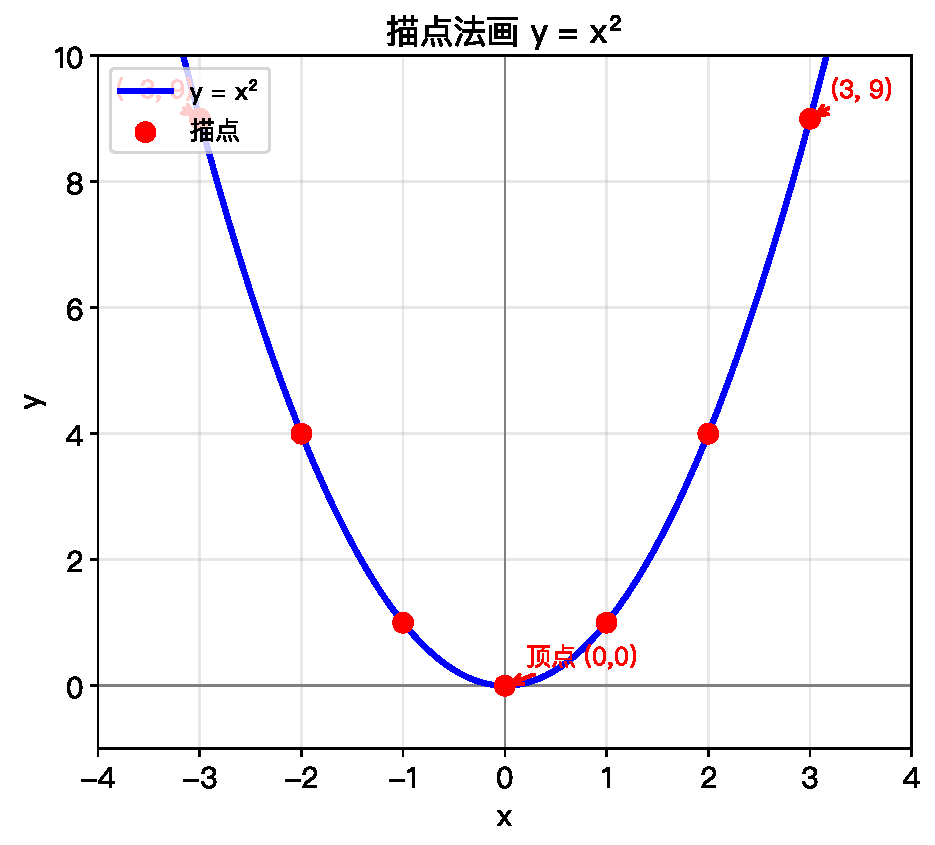
\includegraphics[width=0.55\textwidth]{figures/ch02_sketch_x2.pdf}
\end{center}

你看，这些点排成一条\textbf{抛物线}的形状。

\textbf{从图像能看出什么？}
\begin{itemize}
  \item 最低点在 \((0,0)\)——这是最小值点
  \item 关于 \(y\) 轴对称——左边和右边是对称的
  \item 越往两边走，函数值增长越快
\end{itemize}
\end{examplebox}

\begin{examplebox}[2]
用描点法画 \(y = \dfrac{1}{x}\) 的图像。

\textbf{第1步：列表}

\begin{center}
\begin{tabular}{c|c|c|c|c|c|c}
\(x\) & -3 & -2 & -1 & 1 & 2 & 3 \\
\hline
\(y = 1/x\) & -1/3 & -1/2 & -1 & 1 & 1/2 & 1/3 \\
\end{tabular}
\end{center}

注意：\(x = 0\) 不在定义域内，所以表格中没有 \(x = 0\)。

\textbf{第2步：描点，第3步：连线}

\begin{center}
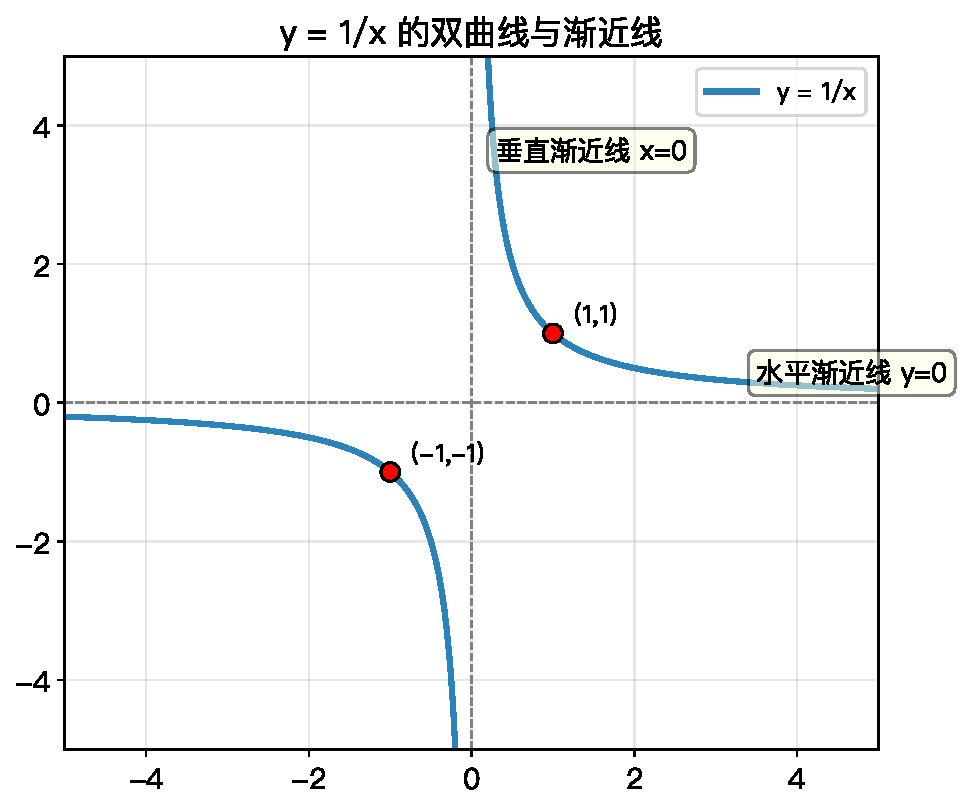
\includegraphics[width=0.5\textwidth]{figures/ch02_reciprocal.pdf}
\end{center}

这个图像叫\textbf{双曲线}（读作 shuāng qū xiàn），它有两条\textbf{渐近线}：
\begin{itemize}
  \item \(x = 0\)（\(y\) 轴）——垂直渐近线，函数在 \(x=0\) 处无定义
  \item \(y = 0\)（\(x\) 轴）——水平渐近线，当 \(x\) 趋向无穷大时函数值趋近 0
\end{itemize}
\end{examplebox}


% ============================================================
\section{六种基本初等函数的图像}
% ============================================================

高中数学中最基本的六种函数，它们的图像必须\textbf{一眼就能认出来}。

\begin{center}
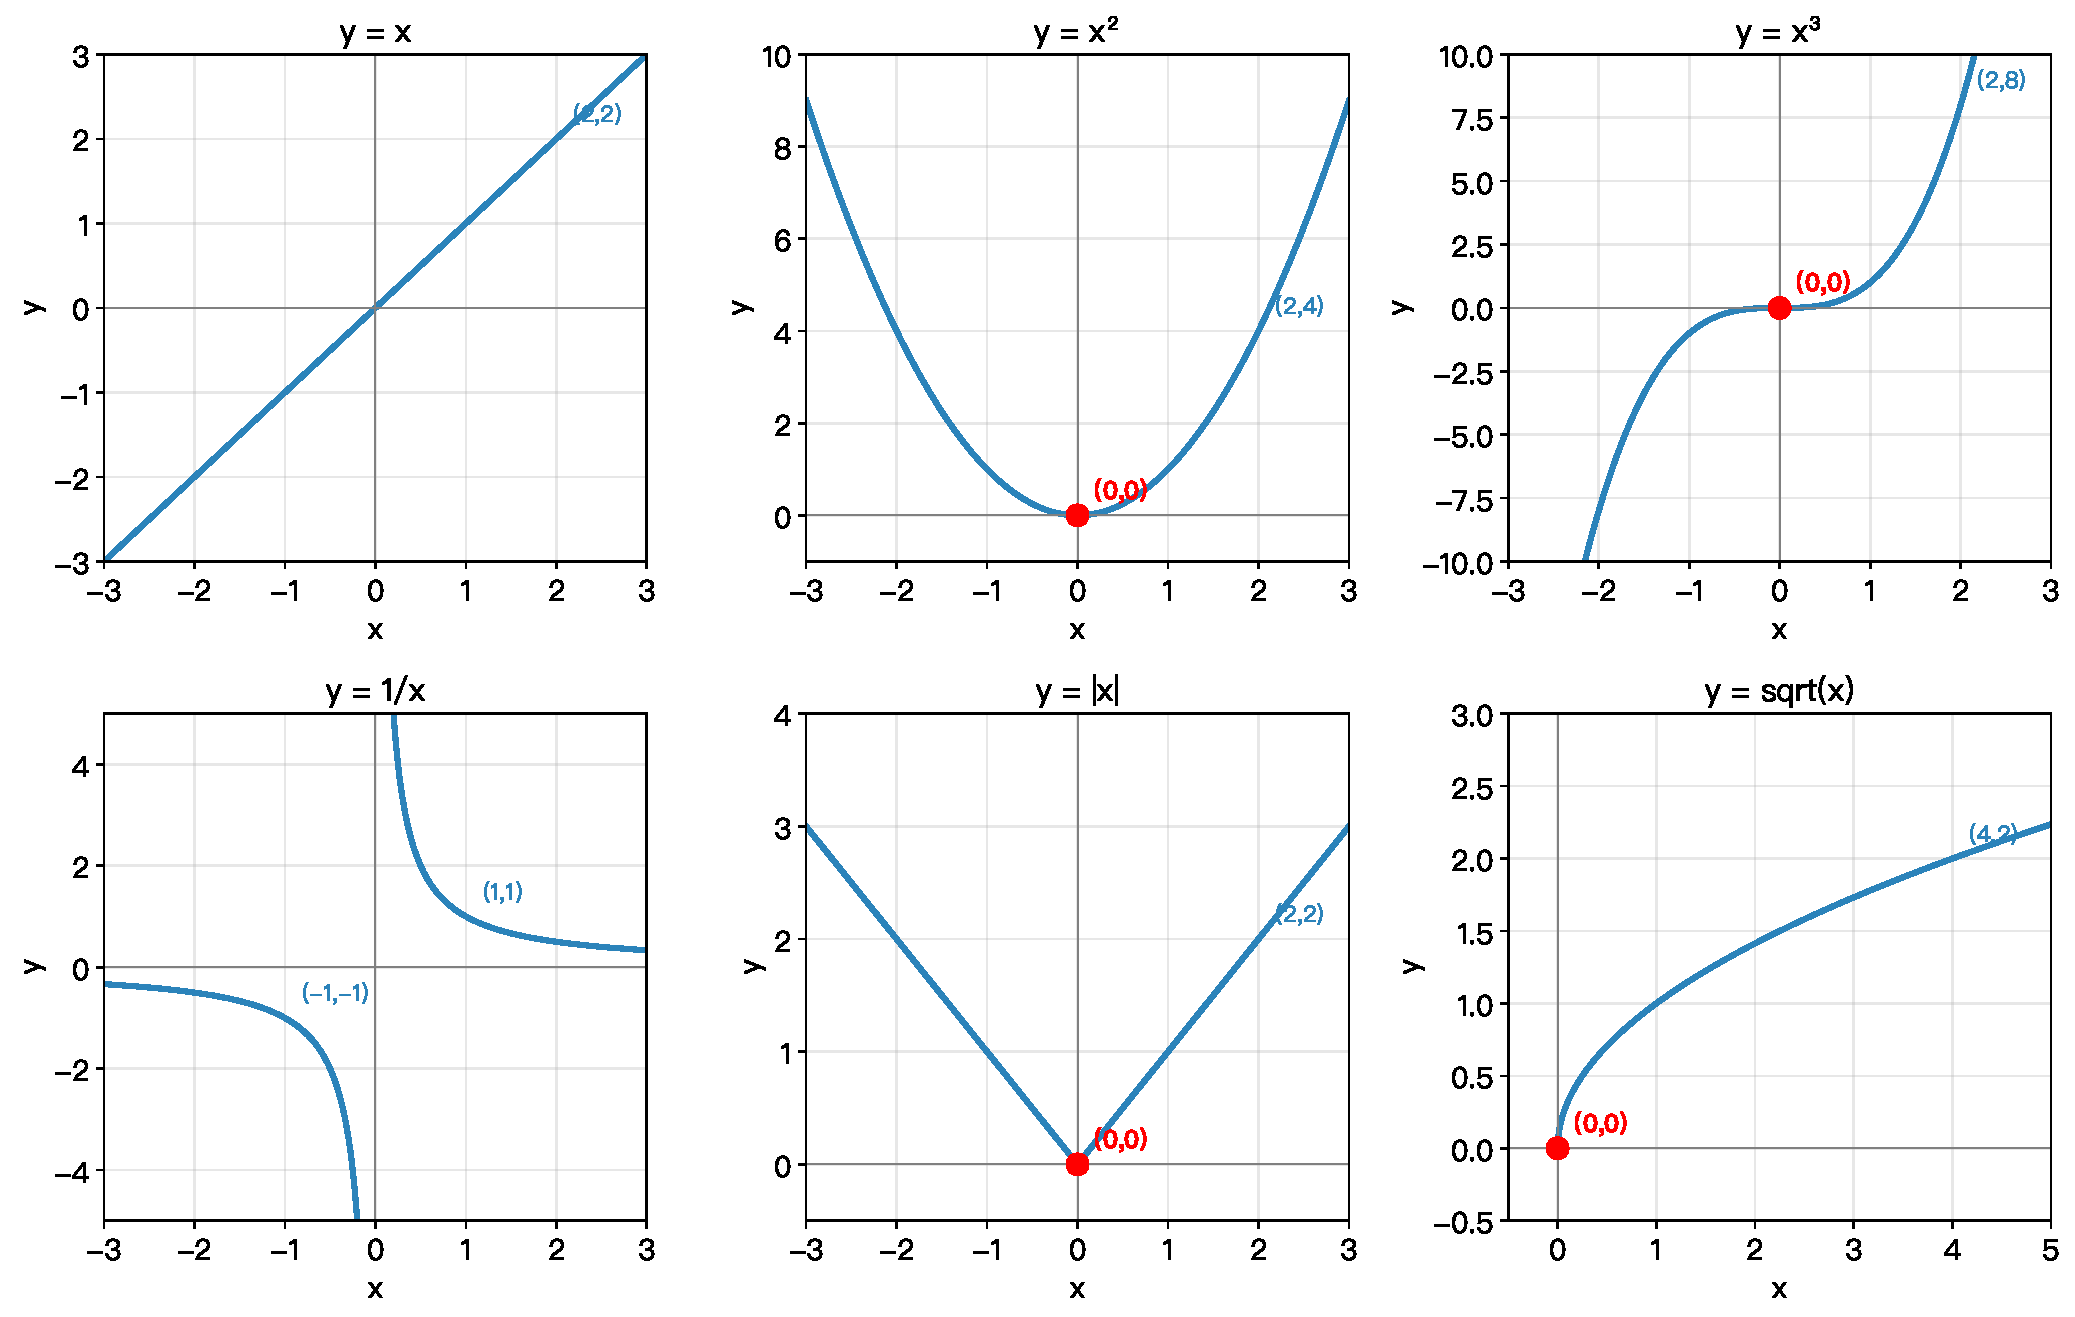
\includegraphics[width=\textwidth]{figures/ch02_six_basic_funcs.pdf}
\end{center}

\begin{examplebox}[3——看图识函数]
对照上图，记住每个函数图像的关键特征：
\begin{enumerate}
  \item \textbf{\(y = x\)}（正比例函数）：通过原点的直线，与 \(x\) 轴成 45° 角
  \item \textbf{\(y = x^2\)}（二次函数）：开口向上的抛物线，顶点在原点
  \item \textbf{\(y = x^3\)}（三次函数）：从左下到右上穿过原点，关于原点对称
  \item \textbf{\(y = 1/x\)}（反比例函数）：双曲线，两条渐近线是坐标轴
  \item \textbf{\(y = |x|\)}（绝对值函数）：V 形，顶点在原点，左右对称
  \item \textbf{\(y = \sqrt{x}\)}（平方根函数）：从原点出发向右延伸，增长速度越来越慢
\end{enumerate}
\end{examplebox}


% ============================================================
\section{从图像读信息——看图说话}
% ============================================================

图像的价值在于：你能\textbf{直接读出}函数的很多重要性质。

\begin{examplebox}[4]
已知函数 \(f(x) = x^3 - x\) 的图像如下：

\begin{center}
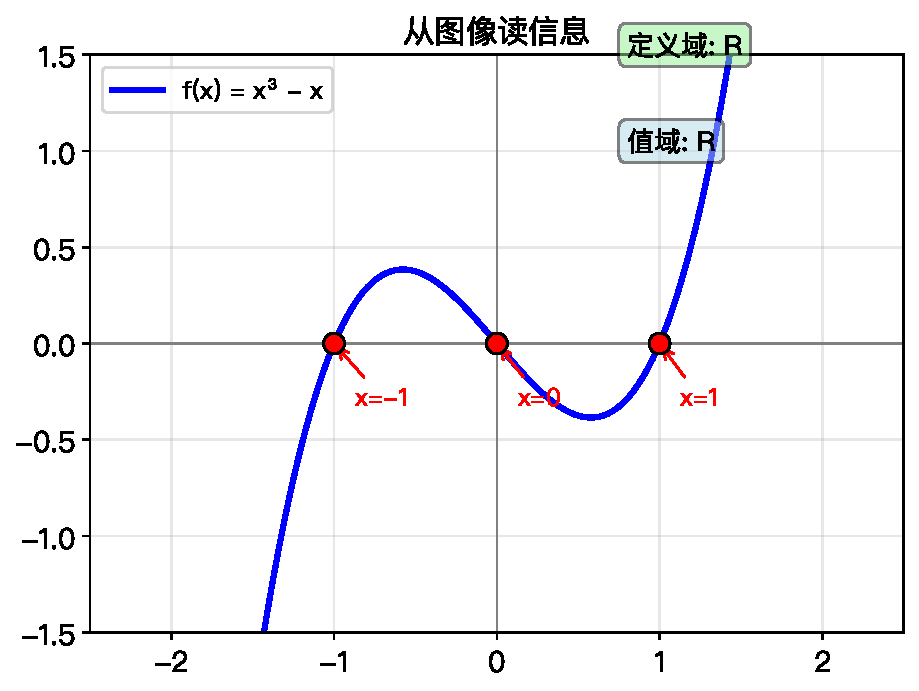
\includegraphics[width=0.5\textwidth]{figures/ch02_read_from_graph.pdf}
\end{center}

从图中可以读出：

\textbf{定义域：} 图像向左右无限延伸 \(\rightarrow\) 定义域为 \(\mathbb{R}\)（全体实数）。

\textbf{值域：} 图像向上下无限延伸 \(\rightarrow\) 值域为 \(\mathbb{R}\)。

\textbf{零点：} 图像与 \(x\) 轴的交点。图中 \(x = -1, 0, 1\) 这三个点处的 \(y = 0\)。\\
验证：\(f(-1) = (-1)^3 - (-1) = -1 + 1 = 0\)，\(f(0) = 0\)，\(f(1) = 1 - 1 = 0\)。

\textbf{单调性：}
\begin{itemize}
  \item 在 \((-\infty, -0.58)\) 上，函数上升（递增）
  \item 在 \((-0.58, 0.58)\) 上，函数下降（递减）
  \item 在 \((0.58, +\infty)\) 上，函数上升（递增）
\end{itemize}
\end{examplebox}

\begin{definitionbox}[从图像读函数性质]
\begin{itemize}
  \item \textbf{定义域}：图像在 \(x\) 轴上的投影范围（看左右到哪）
  \item \textbf{值域}：图像在 \(y\) 轴上的投影范围（看上下到哪）
  \item \textbf{零点}：图像与 \(x\) 轴的交点（\(f(x) = 0\) 的点）
  \item \textbf{单调性}：图像上升 \(\rightarrow\) 递增，图像下降 \(\rightarrow\) 递减
  \item \textbf{最大值/最小值}：图像的最高点/最低点的 \(y\) 坐标
\end{itemize}
\end{definitionbox}


% ============================================================
\section{图像的平移变换——函数搬家}
% ============================================================

在已知一个基本函数图像的基础上，我们可以通过\textbf{平移}得到它的"亲戚"。

\subsection{水平平移：\(y = f(x - a)\)}

\begin{examplebox}[5]
比较 \(y = x^2\) 和 \(y = (x - 2)^2\)：

\begin{center}
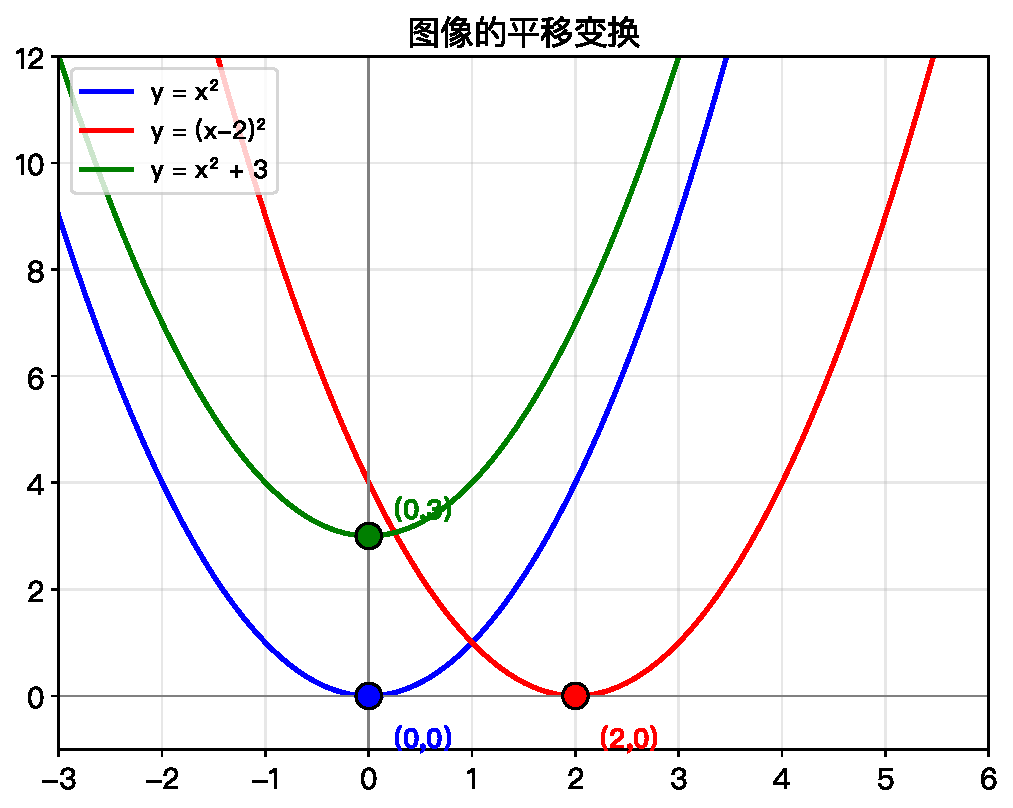
\includegraphics[width=0.55\textwidth]{figures/ch02_translation.pdf}
\end{center}

规律：
\[
y = f(x - a) \text{ 的图像是把 } y = f(x) \text{ 向 \textbf{右} 平移 } a \text{ 个单位}
\]
\[
y = f(x + a) \text{ 的图像是把 } y = f(x) \text{ 向 \textbf{左} 平移 } a \text{ 个单位}
\]

\textbf{注意：} \(x - a\) 是右移，这有点反直觉——因为你想的是"减了 2，应该往左才对"。\\
记忆方法：让 \(x - 2 = 0\) 得 \(x = 2\)，所以顶点从 \(x=0\) 移到了 \(x=2\)——\textbf{右移}。
\end{examplebox}

\subsection{垂直平移：\(y = f(x) + b\)}

容易理解得多：
\[
y = f(x) + b \text{ 的图像是把 } y = f(x) \text{ 向 \textbf{上} 平移 } b \text{ 个单位}
\]
\[
y = f(x) - b \text{ 的图像是把 } y = f(x) \text{ 向 \textbf{下} 平移 } b \text{ 个单位}
\]

\begin{examplebox}[6]
从图中看 \(y = x^2 + 3\)：\\
把 \(y = x^2\) 向上平移 3 个单位，顶点从 \((0,0)\) 移到 \((0,3)\)。
\end{examplebox}


% ============================================================
\section{图像的对称变换——翻转}
% ============================================================

\subsection{关于 \(x\) 轴对称：\(y = -f(x)\)}

\begin{examplebox}[7]
比较 \(y = x^2\) 和 \(y = -x^2\)：

\begin{center}
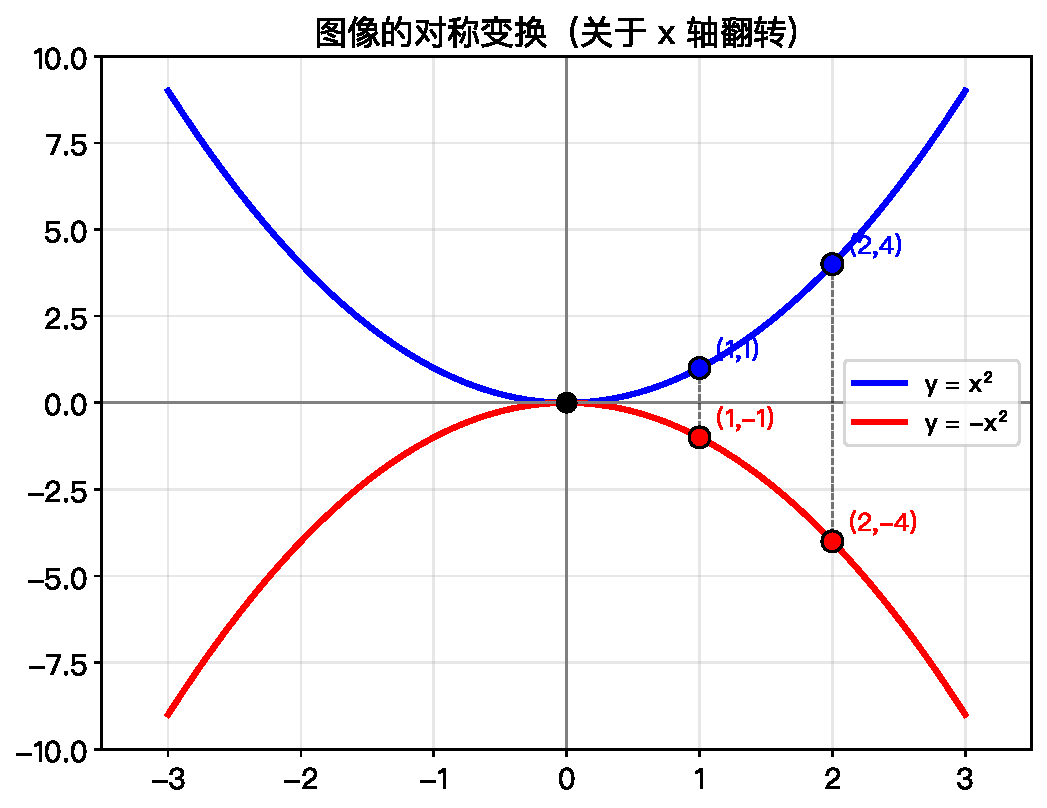
\includegraphics[width=0.55\textwidth]{figures/ch02_symmetry.pdf}
\end{center}

规律：
\[
y = -f(x) \text{ 的图像是把 } y = f(x) \text{ 关于 \(x\) 轴翻转（上下翻转）}
\]

从图中可以看到：\((2, 4)\) 翻到了 \((2, -4)\)，\((1, 1)\) 翻到了 \((1, -1)\)。\\
原来开口向上的抛物线变成了开口向下。
\end{examplebox}

\subsection{关于 \(y\) 轴对称：\(y = f(-x)\)}

\[
y = f(-x) \text{ 的图像是把 } y = f(x) \text{ 关于 \(y\) 轴翻转（左右翻转）}
\]

例：\(y = e^{-x}\) 的图像就是把 \(y = e^x\) 左右翻转（以后学指数函数时会看到）。


% ============================================================
\section{图像的翻折变换——把负的变成正的}
% ============================================================

翻折变换有两种常见形式：

\subsection{\(y = |f(x)|\)——把 \(x\) 轴下方的部分翻到上方}

\begin{examplebox}[8]
比较 \(y = x^2 - 1\) 和 \(y = |x^2 - 1|\)：

\begin{center}
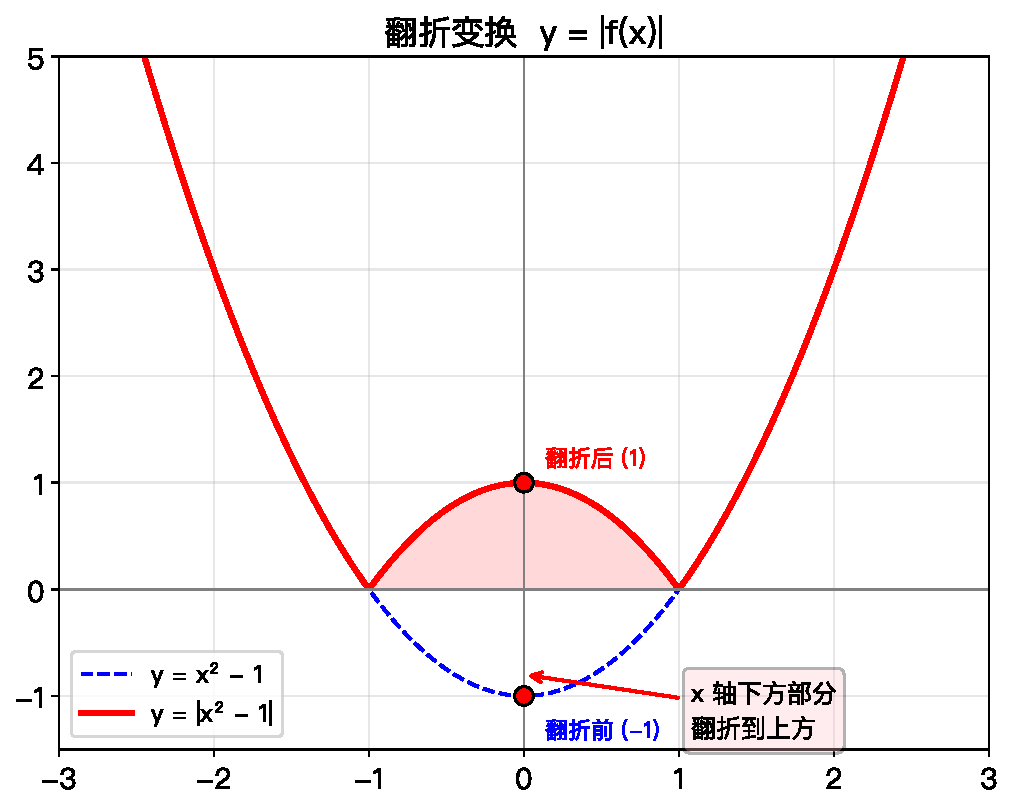
\includegraphics[width=0.55\textwidth]{figures/ch02_abs_flip.pdf}
\end{center}

规律：
\[
y = |f(x)| \text{ 的图像：保留 } y = f(x) \text{ 在 \(x\) 轴上方的部分，}\\
\text{把 \(x\) 轴下方的部分沿 \(x\) 轴翻折到上方}
\]

\textbf{验证：}
\begin{itemize}
  \item \(x = 2\) 时，\(x^2 - 1 = 3\)，\(|3| = 3\)——没变
  \item \(x = 0.5\) 时，\(x^2 - 1 = -0.75\)，\(|-0.75| = 0.75\)——从下方翻到了上方
\end{itemize}
\end{examplebox}

\subsection{\(y = f(|x|)\)——保留右边，对称到左边}

\[
y = f(|x|) \text{ 的图像：保留 } y = f(x) \text{ 在 \(y\) 轴右侧的部分，}\\
\text{去掉左侧部分，把右侧部分关于 \(y\) 轴对称到左侧}
\]


% ============================================================
\section{垂线检验法——判断一个曲线是不是函数}
% ============================================================

\begin{theorembox}[垂线检验法]
在平面上任意画一条竖直线（与 \(y\) 轴平行的直线）：
\begin{itemize}
  \item 如果每条竖直线\textbf{最多}与曲线交于\textbf{一个}点 \(\rightarrow\) 这是\textbf{函数的图像}
  \item 如果某条竖直线与曲线交于\textbf{两个或更多}点 \(\rightarrow\) \textbf{不是函数的图像}
\end{itemize}
\end{theorembox}

\begin{center}
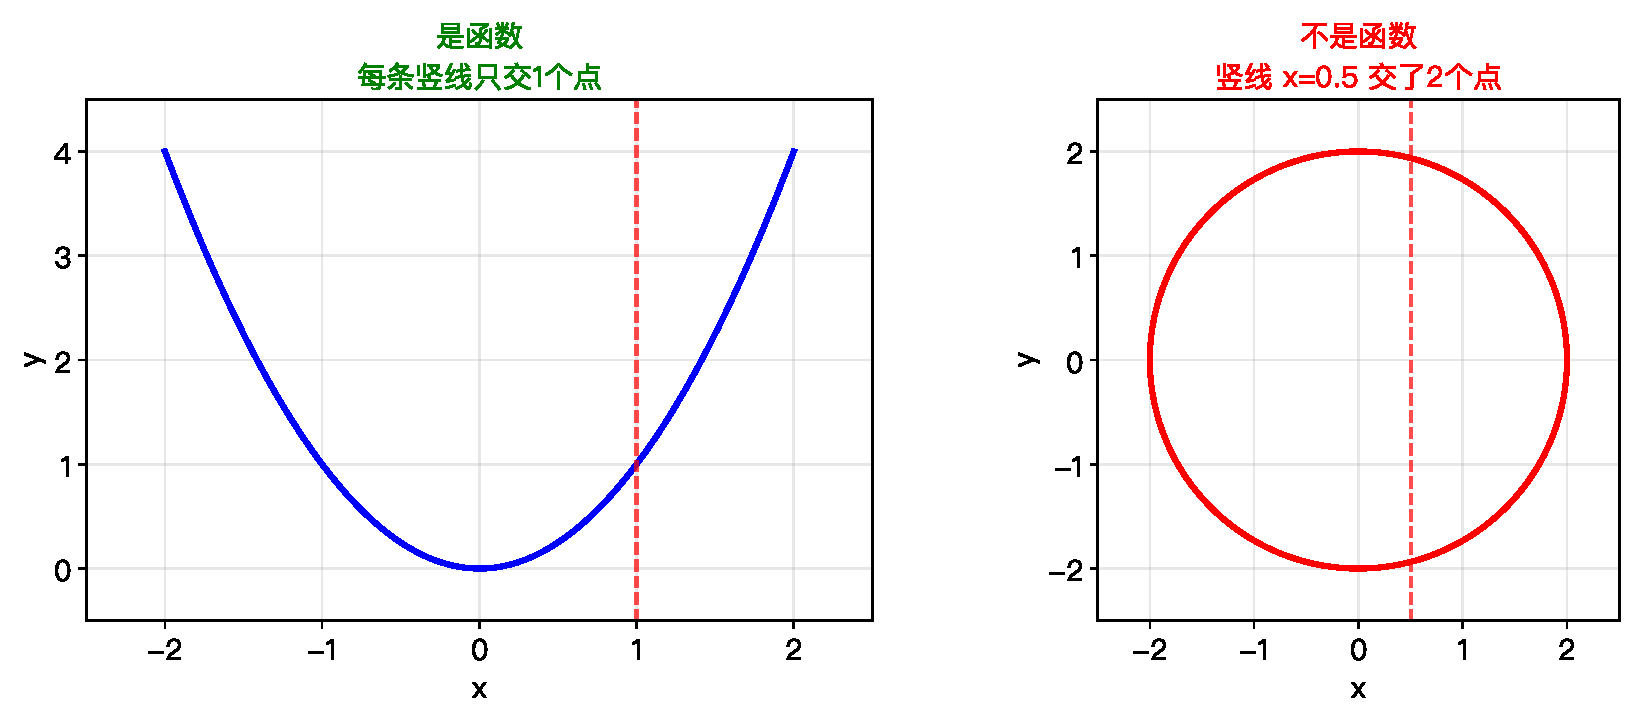
\includegraphics[width=0.75\textwidth]{figures/ch02_vertical_line_test.pdf}
\end{center}

\begin{examplebox}[9]
判断以下曲线是不是函数的图像：
\begin{enumerate}
  \item \textbf{直线 \(y = 2x + 1\)}：任意竖直线只交 1 个点 \(\rightarrow\) 是函数 [OK]
  \item \textbf{圆 \(x^2 + y^2 = 9\)}：竖直线 \(x = 1\) 与圆交于两个点 \(\rightarrow\) 不是函数 [X]
  \item \textbf{抛物线 \(y = x^2\)}：任意竖直线只交 1 个点 \(\rightarrow\) 是函数 [OK]
  \item \textbf{折线 \(y = |x|\)}：任意竖直线只交 1 个点 \(\rightarrow\) 是函数 [OK]
\end{enumerate}
\end{examplebox}


% ============================================================
\section{符号卡片}
% ============================================================

\begin{symbolcard}
\((x, f(x))\) & \verb|(x, f(x))| & 读作"点 x f of x" & 函数图像上的一个点 \\
\(\{\, (x, f(x)) \mid x \in D \,\}\) & \verb+{ (x,f(x)) | x in D }+ & 读作"所有满足...的点" & 函数图像的集合表示 \\
\(y = f(x - a)\) & \verb|y = f(x - a)| & —— & 右移 \(a\) 个单位 \\
\(y = f(x) + b\) & \verb|y = f(x) + b| & —— & 上移 \(b\) 个单位 \\
\(y = -f(x)\) & \verb|y = -f(x)| & —— & 关于 \(x\) 轴对称 \\
\(y = |f(x)|\) & \verb+y = |f(x)|+ & —— & 把 \(x\) 轴下方翻折到上方 \\
\end{symbolcard}


% ============================================================
\section{代码验证}
% ============================================================

\begin{lstlisting}[caption=用 Python 画函数图像]
import numpy as np
import matplotlib.pyplot as plt

# 设置中文字体
plt.rcParams['font.sans-serif'] = ['PingFang SC']
plt.rcParams['axes.unicode_minus'] = False

# 画三个函数在同一坐标系中
x = np.linspace(-4, 4, 400)
plt.figure(figsize=(8, 5))

plt.plot(x, x**2, 'b-', linewidth=2, label='y = x²')
plt.plot(x, x**3, 'r-', linewidth=2, label='y = x³')
plt.plot(x, 2**x, 'g-', linewidth=2, label='y = 2^x')

plt.axhline(0, color='gray', linewidth=0.5)
plt.axvline(0, color='gray', linewidth=0.5)
plt.grid(True, alpha=0.3)
plt.legend(fontsize=12)
plt.title('三个函数图像的对比', fontsize=14)
plt.xlim(-4, 4)
plt.ylim(-5, 20)

# 标注几个关键点
plt.scatter([0], [0], color='black', s=30)
plt.text(0.2, 0.2, 'O', fontsize=12)

plt.tight_layout()
plt.savefig('/tmp/three_funcs.png', dpi=120)
print('图像已保存到 /tmp/three_funcs.png')
\end{lstlisting}

运行结果：在同一个坐标系中画出 \(y=x^2\)、\(y=x^3\)、\(y=2^x\) 三条曲线，直观对比它们的增长速度——你会发现指数函数 \(2^x\) 最终会超过任何幂函数。


% ============================================================
\section{本章小结}
% ============================================================

\begin{progressbox}
\textbf{描点法}：列表 \(\rightarrow\) 描点 \(\rightarrow\) 连线——画任何函数图像的根本方法

\textbf{从图像读信息}：定义域（左右看）、值域（上下看）、零点（与 \(x\) 轴交点）

\textbf{六大基本函数图像}：\(y=x\)（直线）、\(y=x^2\)（抛物线）、\(y=x^3\)（三次曲线）、
\(y=1/x\)（双曲线）、\(y=|x|\)（V形）、\(y=\sqrt{x}\)（半支抛物线）

\textbf{图像变换}：
\begin{itemize}
  \item 平移：\(y = f(x-a)\) 右移，\(y = f(x)+b\) 上移
  \item 对称：\(y = -f(x)\) 关于 \(x\) 轴对称，\(y = f(-x)\) 关于 \(y\) 轴对称
  \item 翻折：\(y = |f(x)|\) 把下方翻到上方
\end{itemize}

\textbf{垂线检验法}：判断曲线是不是函数的最直观方法
\end{progressbox}

\subsection*{通往下一章}

\textbf{这一章}你学会了把函数翻译成图像，也从图像读出函数的信息。

\textbf{下一章}我们学\textbf{幂函数与多项式}——最基本的"弯曲"函数。
你会看到 \(x\) 的指数变化如何改变曲线的形状，以及多项式如何组合出更复杂的曲线。


% ============================================================
% 习题（无竞赛题，极难1道）
% ============================================================
\section{习题}

% ===== 送分 =====

\begin{exercise}[0]
已知函数 \(y = f(x)\) 的图像如下（描述），判断它经过以下哪些点：
\[
A(0,0),\; B(1,2),\; C(-1,-2),\; D(2,4)
\]
(1) \(y = 2x\) \quad (2) \(y = x^2\) \quad (3) \(y = |x|\)
\end{exercise}

\begin{exercise}[0]
看图回答：函数 \(y = x^2\) 的图像与 \(x\) 轴有几个交点？交点的坐标是多少？
\end{exercise}

\begin{exercise}[0]
画出 \(y = x + 1\) 的草图（取 3 个点就够了），并标出它与 \(x\) 轴、\(y\) 轴的交点。
\end{exercise}

\begin{exercise}[0]
判断以下变换是否正确：
\[
y = (x + 3)^2 \text{ 是把 } y = x^2 \text{ 向左平移 3 个单位（是/否）}
\]
\end{exercise}

% ===== 简单 =====

\begin{exercise}[1]
用描点法画出 \(y = 2x - 1\) 的图像（取 \(x = -1, 0, 1\) 三个点）。
\end{exercise}

\begin{exercise}[1]
已知函数 \(y = f(x)\) 的图像向右平移 2 个单位得到 \(y = f(x - 2)\)。\\
如果原来图像上的点 \((1, 3)\) 移到了哪里？点 \((0, 0)\) 呢？
\end{exercise}

\begin{exercise}[1]
下列点中，哪些在 \(y = x^3\) 的图像上？
\[
A(1,1),\; B(-2, -8),\; C(3, 9),\; D(-1, 1),\; E(0,0)
\]
\end{exercise}

\begin{exercise}[1]
函数 \(y = -x^2\) 的图像和 \(y = x^2\) 的图像是什么关系？
\end{exercise}

% ===== 基础 =====

\begin{exercise}[2]
画出下列函数的草图（不用精确，画出大致形状即可）：
\begin{enumerate}
  \item[(1)] \(y = x^2 + 2\)
  \item[(2)] \(y = (x - 1)^2\)
  \item[(3)] \(y = -|x|\)
\end{enumerate}
\end{exercise}

\begin{exercise}[2]
从图像判断：函数 \(y = x^3 - x\) 有几个零点？大致位置在哪里？
\end{exercise}

\begin{exercise}[2]
函数 \(y = \dfrac{1}{x} + 1\) 的图像是把 \(y = \dfrac{1}{x}\) 的图像怎么变换得到的？
它有水平渐近线吗？垂直渐近线呢？
\end{exercise}

\begin{exercise}[2]
已知 \(y = f(x)\) 的图像如下：\\
当 \(x = 0\) 时 \(y = 1\)，当 \(x = 2\) 时 \(y = 3\)，整体是一条直线。\\
写出 \(f(x)\) 的表达式。
\end{exercise}

% ===== 普通 =====

\begin{exercise}[3]
在同一坐标系中画出 \(y = x^2\) 和 \(y = -x^2 + 3\) 的草图，标出顶点坐标。
\end{exercise}

\begin{exercise}[3]
函数 \(y = |x - 1|\) 的图像是什么形状？顶点在哪里？\\
用分段函数表示这个函数。
\end{exercise}

\begin{exercise}[3]
判断以下曲线能否是函数的图像，并说明理由：
\begin{enumerate}
  \item[(1)] 一个完整的椭圆
  \item[(2)] 上半圆（\(y \ge 0\) 的部分）
  \item[(3)] 一条与 \(y\) 轴平行的直线
  \item[(4)] 一条与 \(x\) 轴平行的直线
\end{enumerate}
\end{exercise}

\begin{exercise}[3]
函数 \(y = \dfrac{1}{x - 2}\) 的图像是把 \(y = \dfrac{1}{x}\) 的图像经过什么变换得到的？\\
它的垂直渐近线在哪里？
\end{exercise}

\begin{exercise}[3]
已知 \(f(x) = x^2 - 4x + 3\)。
\begin{enumerate}
  \item[(1)] 配方成 \(f(x) = (x - a)^2 + b\) 的形式
  \item[(2)] 说明它是由 \(y = x^2\) 经过怎样的平移得到的
  \item[(3)] 写出顶点的坐标
  \item[(4)] 写出零点的坐标（提示：解 \(f(x) = 0\)）
\end{enumerate}
\end{exercise}

\begin{exercise}[3]
一个函数的图像经过以下变换后得到新函数，写出新函数的表达式：
\begin{enumerate}
  \item[(1)] \(y = x^2\) 向左平移 3 个单位，再向上平移 1 个单位
  \item[(2)] \(y = \dfrac{1}{x}\) 向右平移 2 个单位，再向下平移 1 个单位
  \item[(3)] \(y = |x|\) 关于 \(x\) 轴对称
\end{enumerate}
\end{exercise}

% ===== 中等 =====

\begin{exercise}[4]
画出 \(y = |x^2 - 4|\) 的草图。\\
提示：先画 \(y = x^2 - 4\)，再把 \(x\) 轴下方的部分翻折到上方。
\end{exercise}

\begin{exercise}[4]
已知函数 \(f(x) = x^3\)。
\begin{enumerate}
  \item[(1)] 写出 \(f(x - 1) + 2\) 的表达式
  \item[(2)] 说明它是由 \(y = x^3\) 经过怎样的变换得到的
  \item[(3)] 原图像上的点 \((2, 8)\) 在新图像上对应的点是什么？
\end{enumerate}
\end{exercise}

\begin{exercise}[4]
函数 \(y = \dfrac{1}{x^2}\) 的图像与 \(y = \dfrac{1}{x}\) 的图像有什么不同？\\
（提示：考虑 \(x\) 为负值时的情况，以及奇偶性）
\end{exercise}

\begin{exercise}[4]
已知 \(f(x) = |x + 1| - |x - 2|\)。
\begin{enumerate}
  \item[(1)] 用分段函数表示 \(f(x)\)（提示：分三段讨论）
  \item[(2)] 画出 \(f(x)\) 的草图
  \item[(3)] 求 \(f(x)\) 的值域
\end{enumerate}
\end{exercise}

\begin{exercise}[4]
一个跳水运动员从 10 米跳台跳下，入水前的高度（米）与时间（秒）的关系近似为：
\[
h(t) = 10 - 5t^2 \quad (0 \le t \le \sqrt{2})
\]
\begin{enumerate}
  \item[(1)] 画出 \(h(t)\) 的图像
  \item[(2)] 从图上读出：\(t = 1\) 秒时的高度是多少？
  \item[(3)] 入水时 \(h = 0\)，从图上看出大约需要多少秒？
\end{enumerate}
\end{exercise}

% ===== 进阶 =====

\begin{exercise}[5]
函数 \(y = \dfrac{ax + b}{cx + d}\)（\(c \neq 0\)，\(ad \neq bc\)）的图像是双曲线。\\
已知 \(y = \dfrac{2x - 1}{x + 1}\)：
\begin{enumerate}
  \item[(1)] 化成 \(y = k + \dfrac{m}{x + 1}\) 的形式（提示：多项式除法）
  \item[(2)] 说明它是由 \(y = \dfrac{1}{x}\) 经过怎样的变换得到的
  \item[(3)] 写出渐近线方程
\end{enumerate}
\end{exercise}

\begin{exercise}[5]
已知函数 \(f(x) = x^2 + 2ax + 3\)（\(a\) 是常数）。
\begin{enumerate}
  \item[(1)] 配方，写出顶点坐标（用 \(a\) 表示）
  \item[(2)] 当 \(a\) 变化时，顶点在什么曲线上运动？
  \item[(3)] 如果 \(f(x)\) 的图像与 \(x\) 轴没有交点，\(a\) 的取值范围是多少？
\end{enumerate}
\end{exercise}

\begin{exercise}[5]
\(y = |x^2 - 2x - 3|\) 的图像与直线 \(y = m\) 有 4 个不同的交点。\\
求 \(m\) 的取值范围。

（提示：先画出 \(y = |x^2 - 2x - 3|\) 的草图，再找水平线与图像交 4 个点的条件。）
\end{exercise}

\begin{exercise}[5]
函数 \(f(x) = \sqrt{x}\) 的图像经过以下变换：
\[
y = \sqrt{x} \;\to\; y = \sqrt{x - 2} \;\to\; y = 3\sqrt{x - 2} \;\to\; y = 3\sqrt{x - 2} + 1
\]
分别说明每一步是什么变换。
\end{exercise}

% ===== 拔高 =====

\begin{exercise}[6]
已知函数 \(f(x) = x^2 + 2|x| - 3\)。
\begin{enumerate}
  \item[(1)] 去掉绝对值，写成分段函数的形式
  \item[(2)] 画出 \(f(x)\) 的完整图像
  \item[(3)] 求 \(f(x)\) 的值域
  \item[(4)] 方程 \(f(x) = k\) 有 4 个不同的实数解，求 \(k\) 的取值范围
\end{enumerate}
\end{exercise}

\begin{exercise}[6]
函数 \(f(x) = \dfrac{x}{|x|}\)（\(x \neq 0\)）的值只有两种可能。
\begin{enumerate}
  \item[(1)] \(f(x)\) 可能的取值是什么？
  \item[(2)] 画出 \(f(x)\) 的图像
  \item[(3)] 这个函数是奇函数还是偶函数？（提示：看 \(f(-x) = ?\)）
\end{enumerate}
\end{exercise}

\begin{exercise}[6]
已知 \(f(x) = |x - 2| + |x + 1| + |x - 3|\)。
\begin{enumerate}
  \item[(1)] 用分段函数表示 \(f(x)\)（提示：分 4 段讨论）
  \item[(2)] 画出 \(f(x)\) 的草图（不要求精确，画出大致形状和关键点即可）
  \item[(3)] 求 \(f(x)\) 的最小值
\end{enumerate}
\end{exercise}

% ===== 极难 =====

\begin{exercise}[7]
已知函数 \(f(x)\) 的定义域为 \(\mathbb{R}\)，且满足：
\[
f(x + y) = f(x) + f(y) \quad \text{对所有实数 } x, y \text{ 成立}
\]
已知 \(f(1) = 1\)。

\begin{enumerate}
  \item[(1)] 求 \(f(0)\)、\(f(2)\)、\(f(-1)\)、\(f(4)\)。
  \item[(2)] 证明 \(f(n) = n\) 对所有整数 \(n\) 成立。
  \item[(3)] 证明 \(f(q) = q\) 对所有有理数 \(q\) 成立。
  \item[(4)] 如果还知道 \(f\) 的图像是连续的（即图像是一条不间断的曲线），
        证明 \(f(x) = x\) 对所有实数 \(x\) 成立。
\end{enumerate}

\textbf{说明：} 这道题把函数方程和图像性质结合起来了。
第(4)问的"连续性"是数学分析的核心概念，这里先作为一个直观概念使用。
\end{exercise}

% ============================================================
% 第3章：幂函数与多项式——变化的"速度"
% ============================================================

\chapter{幂函数与多项式——变化的"速度"}

\begin{applicationbox}
\textbf{学完本章你能做什么？}
\begin{enumerate}
  \item \textbf{学之前}：你知道 \(y = x^2\) 是抛物线，\(y = x^3\) 是三次曲线——但为什么指数不同，曲线长得不一样？
  \item \textbf{学之后}：你能一眼看出一个幂函数或多项式在 \(x\) 很大时的"走向"——向上还是向下？增长多快？
        你还会看到多项式的根如何决定它与 \(x\) 轴的交点。
  \item \textbf{日常例子}：自由落体的距离 \(s = \frac{1}{2}gt^2\) 是 \(t\) 的二次函数；\\
        物体的体积随半径的三次方增长（\(V = \frac{4}{3}\pi r^3\)）。不同指数描述不同的增长速度——这是幂函数的核心。
\end{enumerate}
\end{applicationbox}


% ============================================================
\section{从第2章来——函数的图像告诉我们什么？}
% ============================================================

第2章我们画了六种基本函数的图像，其中最关键的一个区别是\textbf{增长的"速度"}：

\begin{center}
\begin{tabular}{c|c|c}
\textbf{函数} & \textbf{当 \(x\) 很大时的行为} & \textbf{增长"等级"} \\
\hline
\(y = x\) & 直线增长 & 慢 \\
\(y = x^2\) & 抛物线增长（越来越快） & 中等 \\
\(y = x^3\) & 三次方增长（更快） & 快 \\
\end{tabular}
\end{center}

这种"增长等级"就是由\textbf{幂函数的指数}决定的。\\
指数的变化，会彻底改变曲线的形状和行为。


% ============================================================
\section{幂函数的定义}
% ============================================================

\begin{definitionbox}[幂函数]
形如
\[
y = x^n
\]
的函数称为\textbf{幂函数}（读作 mì hán shù，英文 power function），
其中 \(n\) 是\textbf{常数}（可以是整数、分数、正数、负数）。

\textbf{注意：}幂函数的特点是\textbf{底是变量 \(x\)，指数是常数 \(n\)}。
不要和指数函数 \(y = n^x\)（底是常数，指数是变量）搞混。
\end{definitionbox}

\begin{examplebox}[1——幂函数 vs 指数函数]
\begin{center}
\begin{tabular}{c|c|c}
 & \textbf{幂函数} & \textbf{指数函数} \\
\hline
形式 & \(y = x^n\) & \(y = a^x\) \\
例子 & \(y = x^2\)（底变，指数固定） & \(y = 2^x\)（底固定，指数变） \\
图像特征 & 经过 \((1,1)\) & 经过 \((0,1)\) \\
\end{tabular}
\end{center}

\textbf{记忆方法：} "幂"字下面是"幂"——底数像底座（变化），指数像屋顶（固定）。
\end{examplebox}


% ============================================================
\section{正整数幂——指数越大，增长越快}
% ============================================================

当 \(n\) 是正整数（\(n = 1, 2, 3, 4, \ldots\)）时，\(y = x^n\) 是最简单的幂函数。

\begin{examplebox}[2]
在同一坐标系中对比 \(y = x\)、\(y = x^2\)、\(y = x^3\)、\(y = x^4\)：

\begin{center}
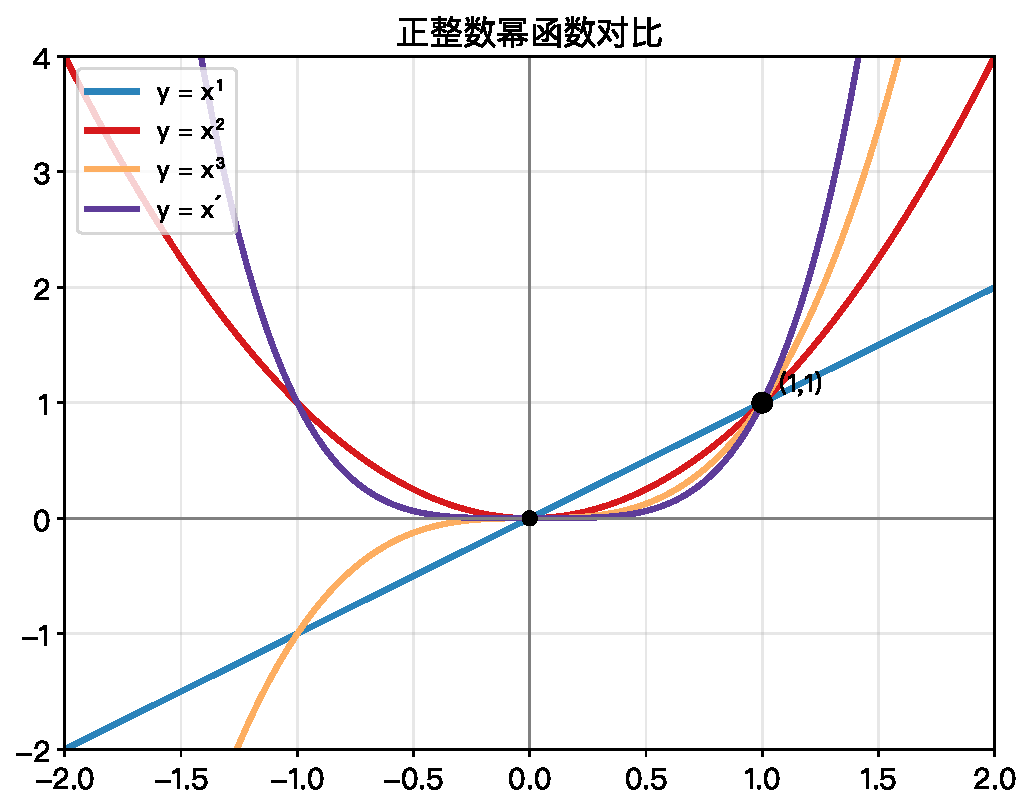
\includegraphics[width=0.6\textwidth]{figures/ch03_positive_powers.pdf}
\end{center}

\textbf{观察规律：}
\begin{enumerate}
  \item 所有图像都经过 \((0,0)\) 和 \((1,1)\)——因为 \(0^n = 0\)，\(1^n = 1\)
  \item 在 \(0 < x < 1\) 区域：指数越大，函数值越小（因为分数越乘越小）
  \item 在 \(x > 1\) 区域：指数越大，增长越快（\(x^4\) 跑得比 \(x^2\) 快得多）
  \item 偶次幂（\(n=2,4\)）的图像关于 \(y\) 轴对称，是\textbf{偶函数}
  \item 奇次幂（\(n=1,3\)）的图像关于原点对称，是\textbf{奇函数}
\end{enumerate}
\end{examplebox}

\begin{definitionbox}[奇函数与偶函数]
\begin{itemize}
  \item \textbf{偶函数}：\(f(-x) = f(x)\)，图像关于 \(y\) 轴对称（如 \(y = x^2\)）
  \item \textbf{奇函数}：\(f(-x) = -f(x)\)，图像关于原点对称（如 \(y = x^3\)）
\end{itemize}
\end{definitionbox}

\begin{examplebox}[3——奇偶性的直观理解]
\begin{itemize}
  \item \(y = x^2\)：左边和右边一样高 \(\rightarrow\) 偶函数
  \item \(y = x^3\)：左边(负)是右边(正)的倒影 \(\rightarrow\) 奇函数
  \item \(y = x\)（直线）：左边低右边高，经过原点 \(\rightarrow\) 奇函数
\end{itemize}
\end{examplebox}


% ============================================================
\section{正偶次幂与正奇次幂的"走向"}
% ============================================================

对于正整数幂，指数是奇数还是偶数，决定了函数图像\textbf{两端的走向}。

\begin{center}
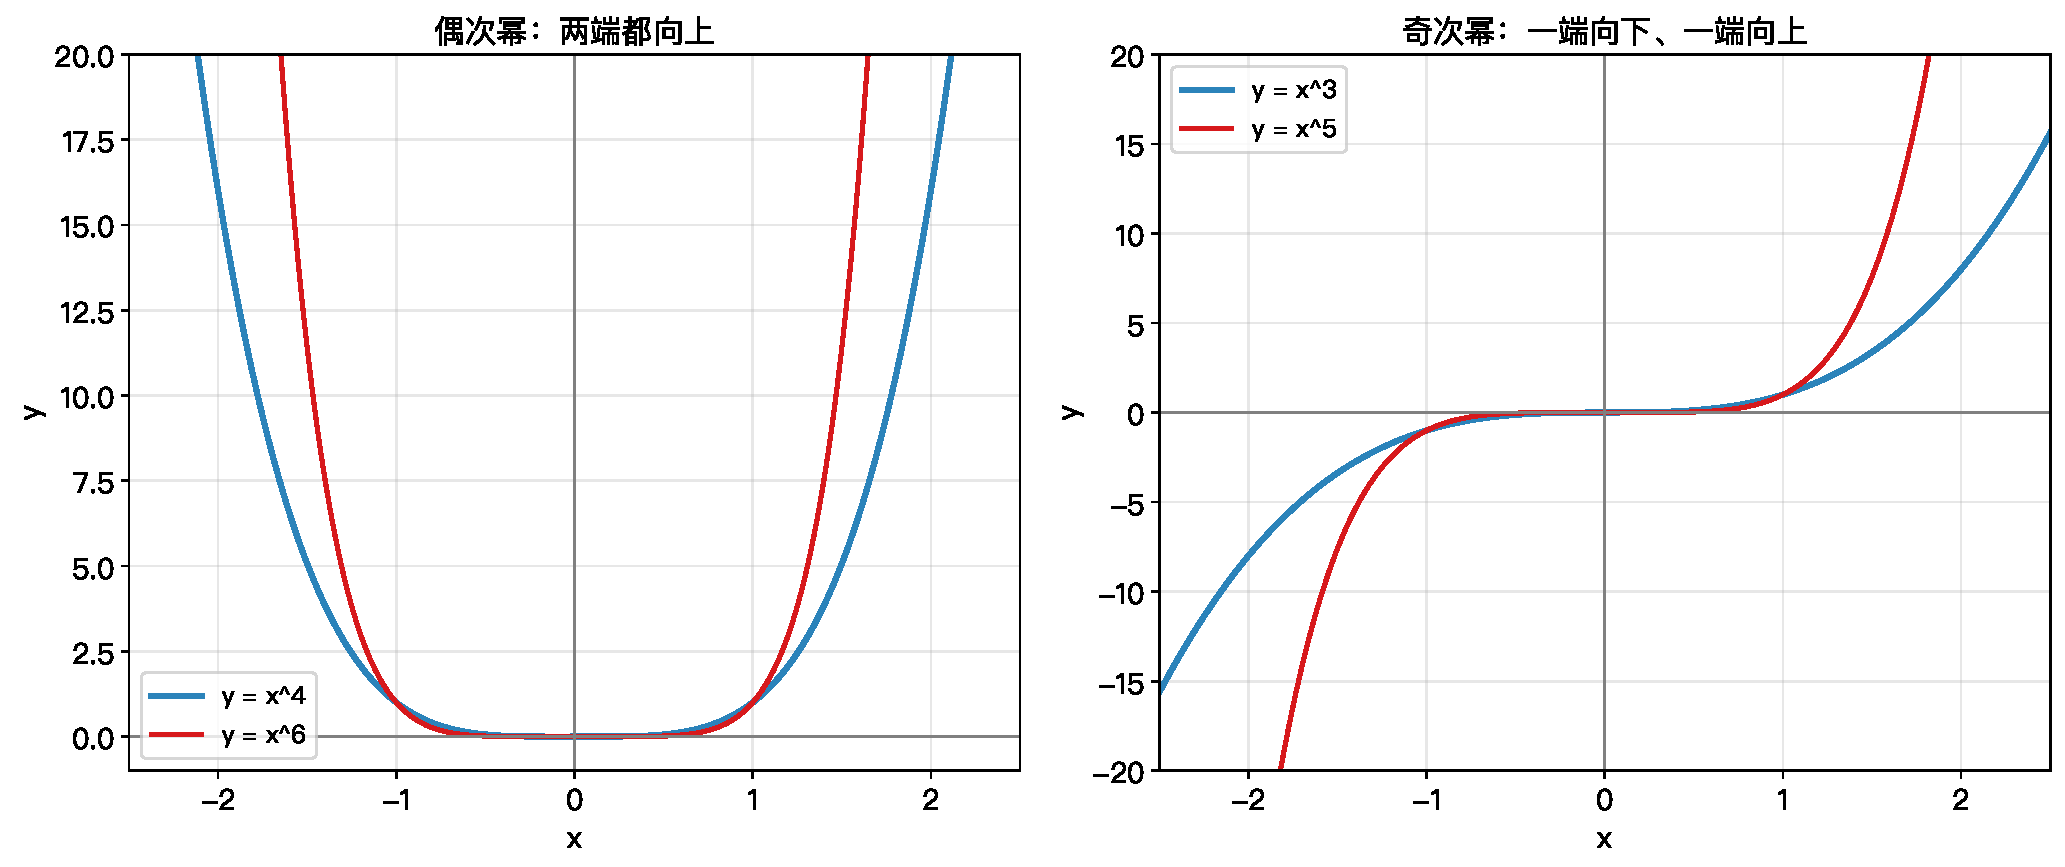
\includegraphics[width=0.75\textwidth]{figures/ch03_even_vs_odd.pdf}
\end{center}

\begin{definitionbox}[幂函数两端走向的规律]
对于 \(y = x^n\)（\(n\) 为正整数）：
\begin{center}
\begin{tabular}{c|c|c}
 & \textbf{\(x \to -\infty\)（左端）} & \textbf{\(x \to +\infty\)（右端）} \\
\hline
\(n\) 为偶数 & \(y \to +\infty\)（向上） & \(y \to +\infty\)（向上） \\
\(n\) 为奇数 & \(y \to -\infty\)（向下） & \(y \to +\infty\)（向上） \\
\end{tabular}
\end{center}

\textbf{记忆口诀：} 偶次幂"两头翘"，奇次幂"一低一高"。
\end{definitionbox}


% ============================================================
\section{负整数幂——倒数关系}
% ============================================================

当 \(n\) 是负整数时，幂函数变成\textbf{分式形式}：
\[
x^{-n} = \frac{1}{x^n}
\]

\begin{examplebox}[4]
对比 \(y = \dfrac{1}{x}\)（即 \(x^{-1}\)）和 \(y = \dfrac{1}{x^2}\)（即 \(x^{-2}\)）：

\begin{center}
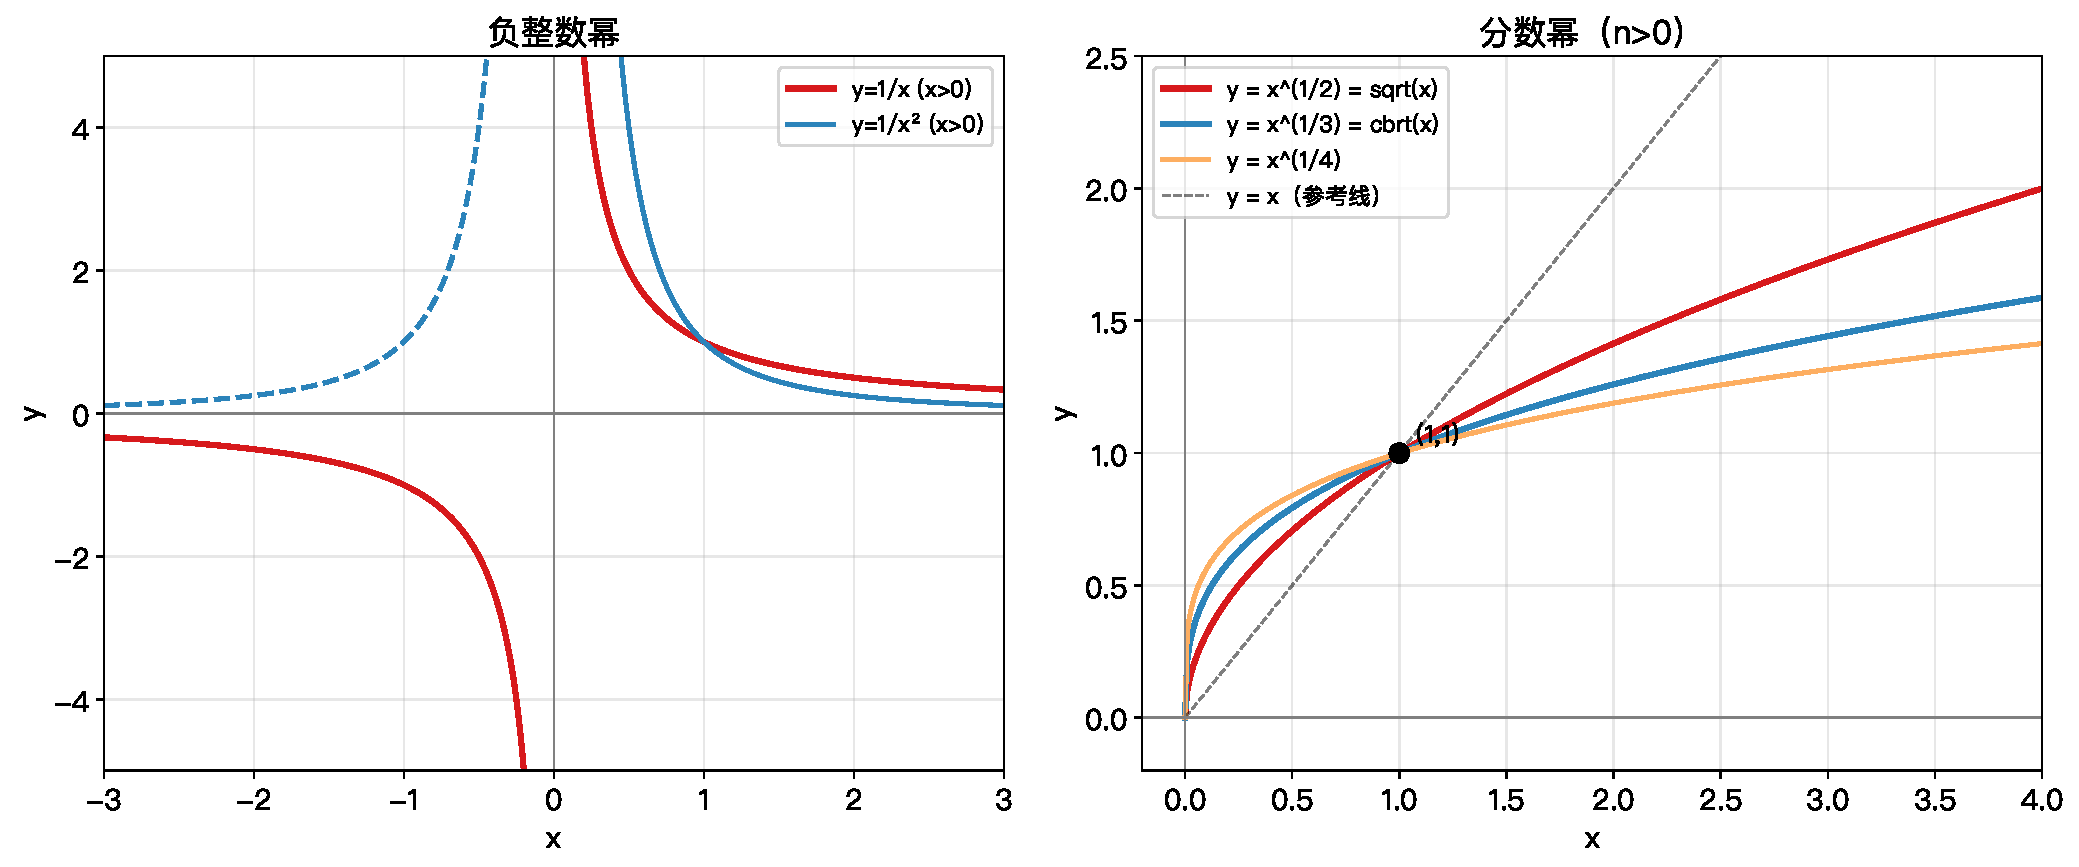
\includegraphics[width=0.55\textwidth]{figures/ch03_power_variants.pdf}
\end{center}

\textbf{关键区别：}
\begin{enumerate}
  \item 定义域：\(x \neq 0\)（分母不能为 0）
  \item \(y = 1/x\)（奇函数）：关于原点对称，图像穿过原点两侧
  \item \(y = 1/x^2\)（偶函数）：关于 \(y\) 轴对称，两侧都在 \(x\) 轴上方
  \item 当 \(x \to \pm\infty\) 时，\(y \to 0\)（水平渐近线 \(y = 0\)）
  \item 当 \(x \to 0\) 时，\(|y| \to \infty\)（垂直渐近线 \(x = 0\)）
\end{enumerate}
\end{examplebox}


% ============================================================
\section{分数幂——根号形式}
% ============================================================

当 \(n\) 是分数时，幂函数变成\textbf{根号形式}：
\[
x^{1/m} = \sqrt[m]{x}
\]

\begin{examplebox}[5]
对比 \(y = x^{1/2} = \sqrt{x}\)、\(y = x^{1/3}\)、\(y = x^{1/4}\)：

\begin{center}
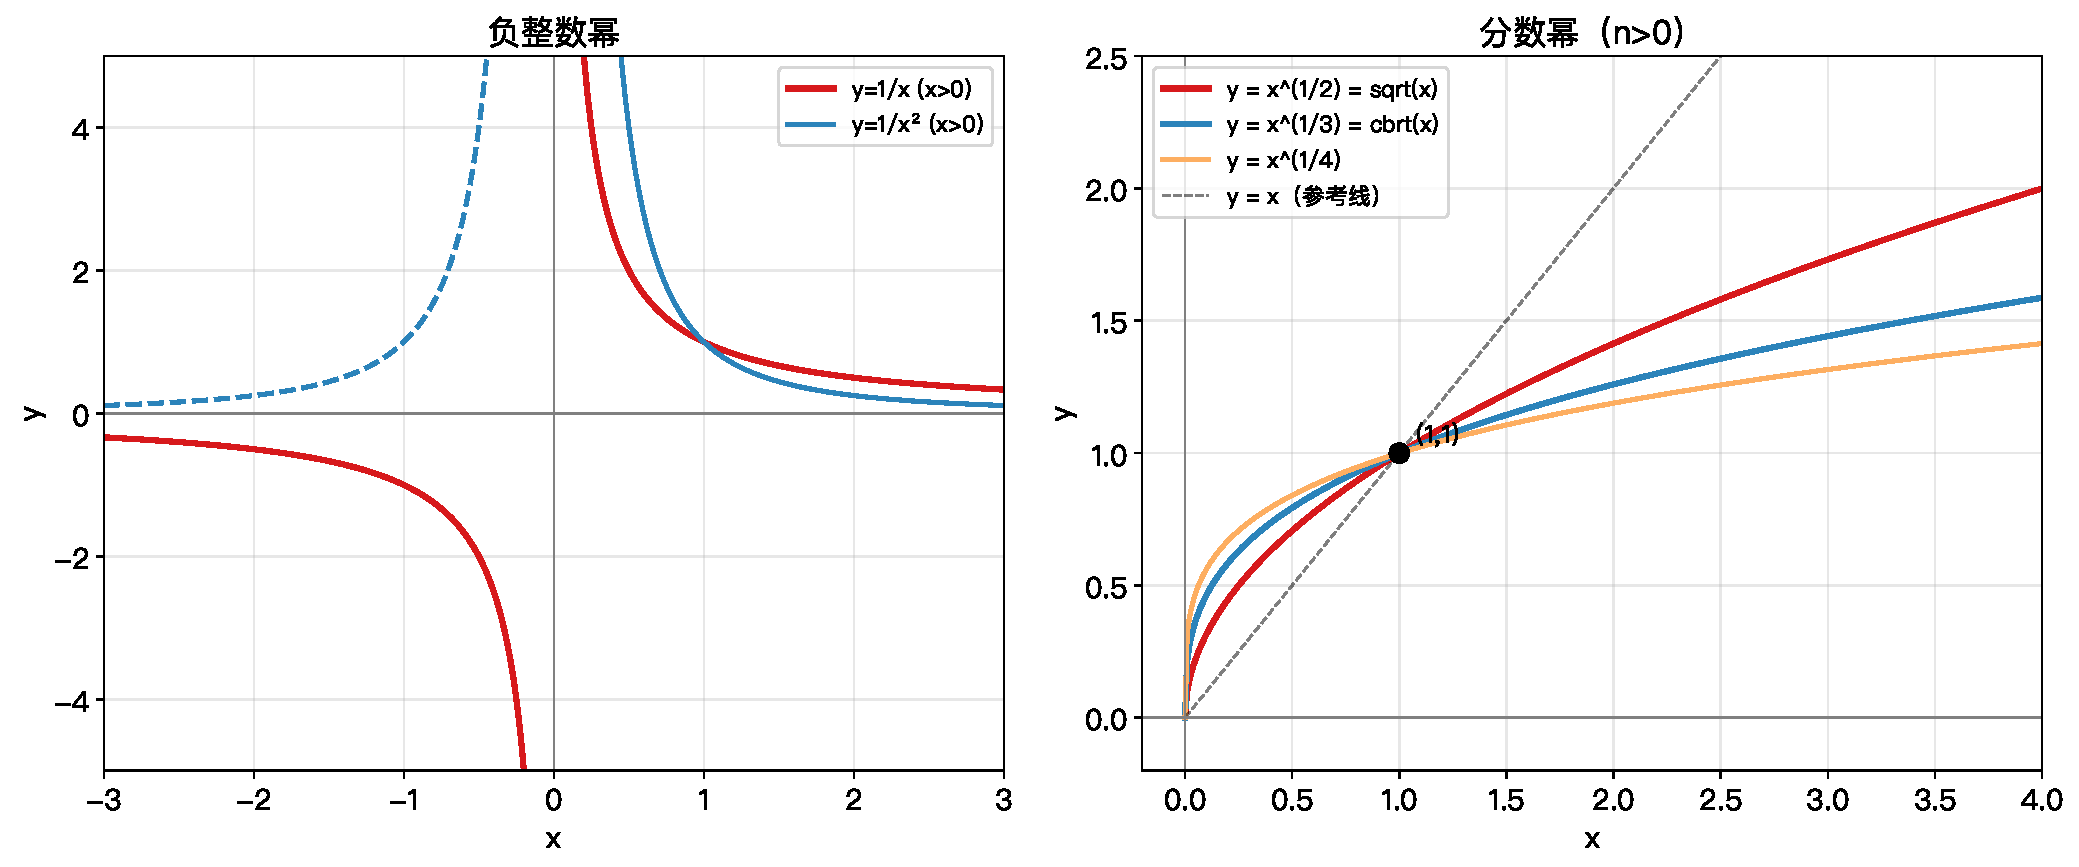
\includegraphics[width=0.55\textwidth]{figures/ch03_power_variants.pdf}
\end{center}

\textbf{规律：}
\begin{enumerate}
  \item 定义域：偶次根号（\(x^{1/2}, x^{1/4}\)）要求 \(x \ge 0\)；奇次根号（\(x^{1/3}\)）定义域为全体实数
  \item 所有分数幂都经过 \((0,0)\) 和 \((1,1)\)
  \item 在 \(x > 1\) 区域：指数越小，图像越靠近 \(x\) 轴（增长越慢）
  \item 分数幂的增长速度\textbf{慢于}直线 \(y = x\)——所以 \(\sqrt{x}\) 比 \(x\) 增长得慢
\end{enumerate}
\end{examplebox}


% ============================================================
\section{幂的运算规则}
% ============================================================

学习多项式之前，需要先巩固幂的运算。

\begin{definitionbox}[幂的运算法则]
设 \(a > 0\)，\(b > 0\)，\(m, n\) 为实数：
\begin{align*}
  a^m \cdot a^n &= a^{m+n} \quad &\text{（同底相乘，指数相加）} \\
  \frac{a^m}{a^n} &= a^{m-n} \quad &\text{（同底相除，指数相减）} \\
  (a^m)^n &= a^{mn} \quad &\text{（幂的乘方，指数相乘）} \\
  (ab)^n &= a^n \cdot b^n \quad &\text{（积的乘方，分别乘方）} \\
  a^{-n} &= \frac{1}{a^n} \quad &\text{（负指数 = 倒数）} \\
  a^{1/n} &= \sqrt[n]{a} \quad &\text{（分数指数 = 根号）}
\end{align*}
\end{definitionbox}

\begin{examplebox}[6——幂运算练习]
计算：
\[
(1)\; 2^3 \cdot 2^4 \qquad (2)\; \frac{3^5}{3^2} \qquad (3)\; (2^2)^3 \qquad (4)\; 8^{2/3}
\]

解：
\[
\begin{aligned}
(1)&\; 2^3 \cdot 2^4 = 2^{3+4} = 2^7 = 128 \\
(2)&\; \frac{3^5}{3^2} = 3^{5-2} = 3^3 = 27 \\
(3)&\; (2^2)^3 = 2^{2\times3} = 2^6 = 64 \\
(4)&\; 8^{2/3} = (8^{1/3})^2 = (\sqrt[3]{8})^2 = 2^2 = 4
\end{aligned}
\]
\end{examplebox}


% ============================================================
\section{多项式函数——幂函数的组合}
% ============================================================

把多个幂函数加起来，就得到了\textbf{多项式}。

\begin{definitionbox}[多项式函数]
形如
\[
P(x) = a_n x^n + a_{n-1} x^{n-1} + \cdots + a_1 x + a_0
\]
的函数称为\textbf{多项式函数}（读作 duō xiàng shì，英文 polynomial），
其中：
\begin{itemize}
  \item \(n\) 是\textbf{最高次数}（多项式的\textbf{次数}，degree）
  \item \(a_n\) 是\textbf{首项系数}（\(a_n \neq 0\)）
  \item \(a_0\) 是\textbf{常数项}
  \item 每一项 \(a_k x^k\) 是一个\textbf{单项式}
\end{itemize}
\end{definitionbox}

\begin{examplebox}[7——多项式举例]
\begin{align*}
  P(x) &= 3x^2 - 2x + 1 \quad &\text{二次多项式（首项系数 3，常数项 1）} \\
  Q(x) &= x^3 - 4x \quad &\text{三次多项式（缺 \(x^2\) 和常数项）} \\
  R(x) &= (x+1)(x-2)(x+3) \quad &\text{因式分解形式的三次多项式}
\end{align*}
\end{examplebox}


% ============================================================
\section{多项式的根——与 \(x\) 轴的交点}
% ============================================================

\begin{definitionbox}[多项式的根]
如果 \(P(r) = 0\)，则称 \(r\) 是多项式 \(P(x)\) 的\textbf{根}（读作 gēn，英文 root），
也叫\textbf{零点}（zero）。

几何意义：根就是函数图像与 \(x\) 轴交点的横坐标。
\end{definitionbox}

\begin{examplebox}[8]
多项式 \(f(x) = (x+2)(x-1)(x-3)\)：

\begin{center}
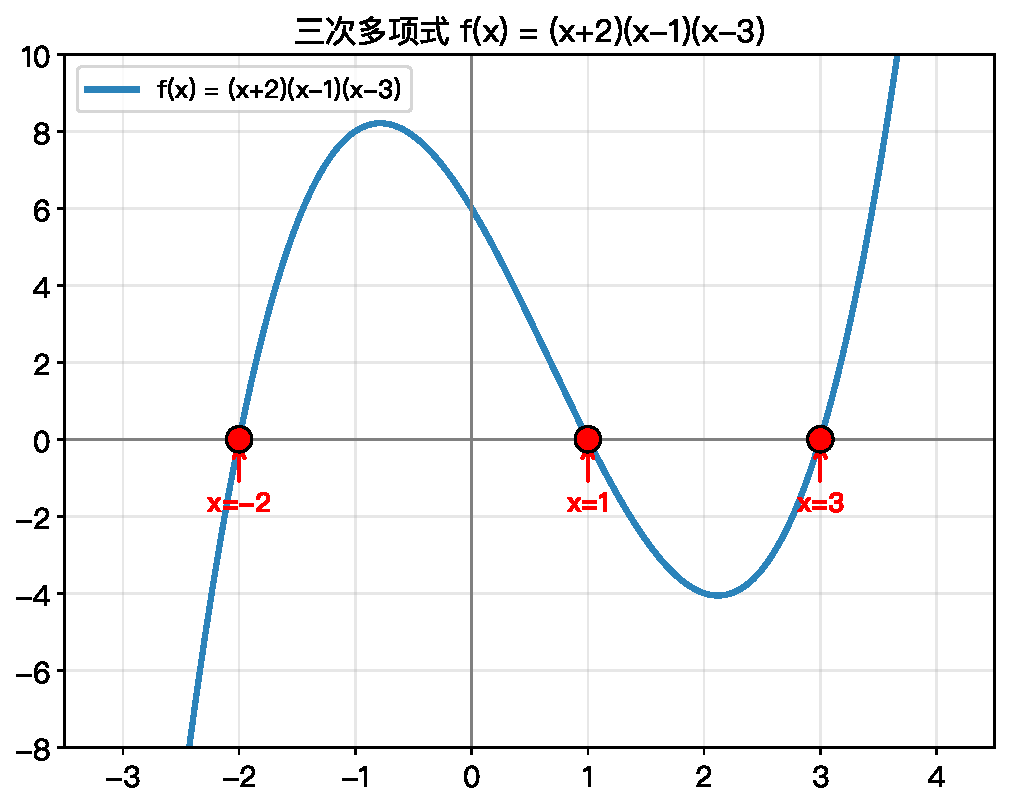
\includegraphics[width=0.6\textwidth]{figures/ch03_cubic_polynomial.pdf}
\end{center}

从图上一眼看出：
\begin{itemize}
  \item 根为 \(x = -2\)、\(x = 1\)、\(x = 3\)（三个根都是\textbf{单根}）
  \item 在根处，图像\textbf{穿过} \(x\) 轴（从一侧到另一侧）
  \item 三次多项式最多有 3 个根
\end{itemize}
\end{examplebox}

\begin{notebox}
多项式的\textbf{次数决定了最多有多少个根}：
\[
\text{\(n\) 次多项式最多有 \(n\) 个实数根}
\]
（可以有不到 \(n\) 个，因为有些根可能是复数——以后学。）
\end{notebox}


% ============================================================
\section{重根——图像"弹回"不穿过}
% ============================================================

如果多项式中某个因式出现了多次，这个根就叫做\textbf{重根}。

\begin{examplebox}[9]
对比单根和重根的行为：

\begin{center}
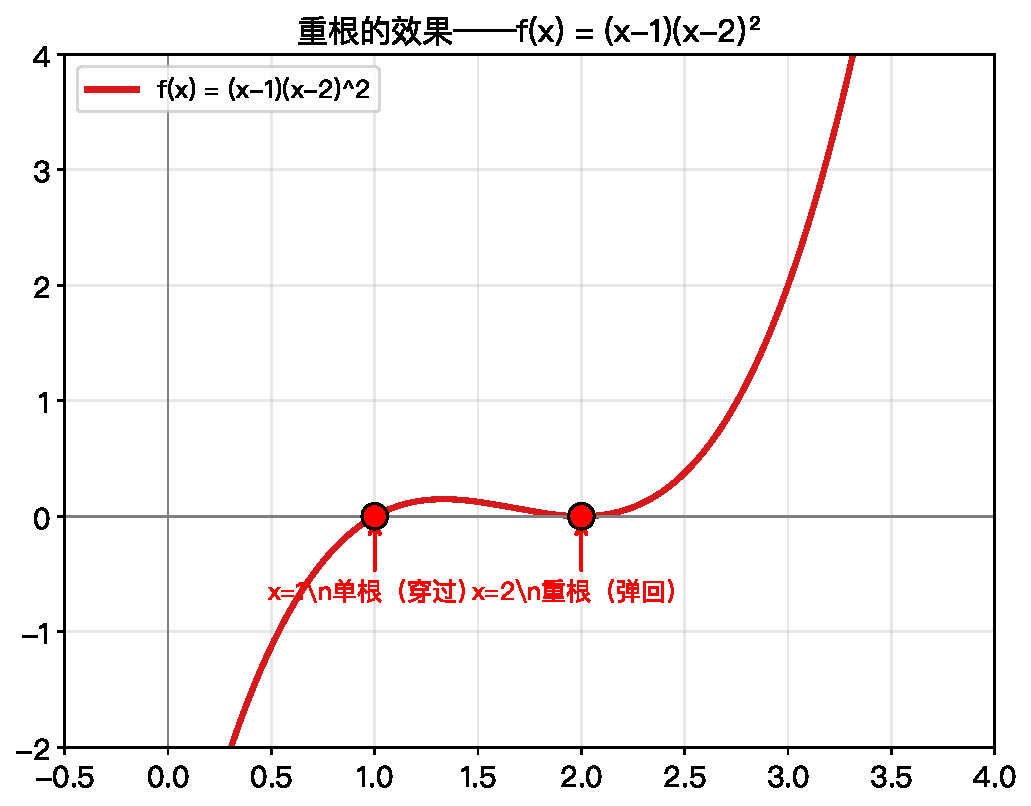
\includegraphics[width=0.6\textwidth]{figures/ch03_double_root.pdf}
\end{center}

\(f(x) = (x-1)(x-2)^2\)：
\begin{itemize}
  \item \(x = 1\)（单根）：图像\textbf{穿过} \(x\) 轴
  \item \(x = 2\)（二重根）：图像\textbf{碰到} \(x\) 轴然后\textbf{弹回}（不穿过）
\end{itemize}

\textbf{规律：}
\begin{center}
\begin{tabular}{c|c}
\textbf{重数} & \textbf{图像行为} \\
\hline
奇数次重根（单根、三重根等） & 穿过 \(x\) 轴 \\
偶数次重根（二重、四重根等） & 碰到 \(x\) 轴弹回 \\
\end{tabular}
\end{center}
\end{examplebox}


% ============================================================
\section{多项式的运算}
% ============================================================

\begin{examplebox}[10——多项式乘法]
展开 \((x+1)(x-2)(x+3)\)：

\[
\begin{aligned}
(x+1)(x-2)(x+3) &= (x^2 - 2x + x - 2)(x+3) \\
&= (x^2 - x - 2)(x+3) \\
&= x^3 + 3x^2 - x^2 - 3x - 2x - 6 \\
&= x^3 + 2x^2 - 5x - 6
\end{aligned}
\]

\textbf{验证：} 当 \(x = 1\) 时，原式 \((2)(-1)(4) = -8\)，展开式 \(1 + 2 - 5 - 6 = -8\) [OK]
\end{examplebox}

\begin{examplebox}[11——多项式除法（综合除法）]
用 \(x-2\) 除 \(x^3 + 2x^2 - 5x - 6\)：

\[
x^3 + 2x^2 - 5x - 6 = (x-2)(x^2 + 4x + 3)
\]

验证：\((x-2)(x^2 + 4x + 3) = x^3 + 4x^2 + 3x - 2x^2 - 8x - 6 = x^3 + 2x^2 - 5x - 6\) [OK]

所以 \(x=2\) 是多项式的一个根（\(f(2) = 8 + 8 - 10 - 6 = 0\)）。
\end{examplebox}

\begin{theorembox}[余数定理]
多项式 \(P(x)\) 除以 \((x-a)\) 的\textbf{余数}就是 \(P(a)\)。

特别地，如果 \(P(a) = 0\)，那么 \((x-a)\) 是 \(P(x)\) 的一个因式。
\end{theorembox}


% ============================================================
\section{符号卡片}
% ============================================================

\begin{symbolcard}
\(x^n\) & \verb|x^n| & 读作"x 的 n 次方" & 幂函数，底 \(x\) 指数 \(n\) \\
\(P(x)\) & \verb|P(x)| & 读作"P of x" & 多项式函数 \\
\(a_n x^n\) & \verb|a_n x^n| & —— & 多项式的第 \(n\) 次项 \\
\(r\) 是 \(P\) 的根 & \verb|P(r)=0| & 读作"P of r 等于 0" & \(r\) 使多项式值为 0 \\
重根 & —— & 读作"chóng gēn" & 因式出现多次的根 \\
\end{symbolcard}


% ============================================================
\section{代码验证}
% ============================================================

\begin{lstlisting}[caption=幂函数与多项式的数值验证]
import numpy as np

# 1. 验证幂函数经过 (1,1)
print("=== 所有幂函数都经过 (1,1) ===")
for n in [1, 2, 3, 4, -1, -2, 0.5]:
    print(f"  n={n:4.1f}:  1^{n} = {1**n}")

print()

# 2. 多项式的根
def f(x):
    return (x + 2) * (x - 1) * (x - 3)

print("=== 多项式的根 ===")
for test_x in [-2, 1, 3]:
    print(f"  f({test_x}) = {f(test_x)}  (应为0)")

print()

# 3. 奇函数性质验证：f(-x) = -f(x)
print("=== 奇函数验证 ===")
for x in [1, 2, 3.5]:
    lhs = x**3          # f(x) = x^3
    rhs_pos = x**3
    rhs_neg = (-x)**3
    print(f"  x={x:3.1f}:  ({x})^3 = {rhs_pos:6.1f},  ({-x})^3 = {rhs_neg:6.1f} = -{rhs_pos}")

print()

# 4. 偶函数验证：f(-x) = f(x)
print("=== 偶函数验证 ===")
for x in [1, 2, 3.5]:
    lhs = x**2
    rhs = (-x)**2
    print(f"  x={x:3.1f}:  ({x})^2 = {lhs:4.1f},  ({-x})^2 = {rhs:4.1f}  (相等)")
\end{lstlisting}

运行结果：
\begin{lstlisting}[frame=none,backgroundcolor={},numbers=none]
=== 所有幂函数都经过 (1,1) ===
  n= 1.0:  1^1 = 1
  n= 2.0:  1^2 = 1
  n= 3.0:  1^3 = 1
  n= 4.0:  1^4 = 1
  n=-1.0:  1^-1 = 1
  n=-2.0:  1^-2 = 1
  n= 0.5:  1^0.5 = 1

=== 多项式的根 ===
  f(-2) = 0  (应为0)
  f(1) = 0  (应为0)
  f(3) = 0  (应为0)

=== 奇函数验证 ===
  x=1.0:  (1)^3 =    1.0,  (-1)^3 =   -1.0 = -1.0
  x=2.0:  (2)^3 =    8.0,  (-2)^3 =   -8.0 = -8.0
  x=3.5:  (3.5)^3 =   42.9,  (-3.5)^3 =  -42.9 = -42.9

=== 偶函数验证 ===
  x=1.0:  (1)^2 = 1.0,  (-1)^2 = 1.0  (相等)
  x=2.0:  (2)^2 = 4.0,  (-2)^2 = 4.0  (相等)
  x=3.5:  (3.5)^2 = 12.2,  (-3.5)^2 = 12.2  (相等)
\end{lstlisting}


% ============================================================
\section{本章小结}
% ============================================================

\begin{progressbox}
\textbf{幂函数} \(y = x^n\)：底变、指数固定。所有幂函数经过 \((1,1)\)。

\textbf{指数 }\(n\) \textbf{决定行为}：
\begin{itemize}
  \item 正整数：\(n\) 越大增长越快，偶次幂"两头翘"，奇次幂"一低一高"
  \item 负整数：\(x^{-n} = 1/x^n\)，有渐近线 \(x=0\) 和 \(y=0\)
  \item 分数：\(x^{1/n} = \sqrt[n]{x}\)，增长慢于直线
\end{itemize}

\textbf{奇偶性}：\(f(-x) = f(x)\)（偶，关于 \(y\) 轴对称）
vs \(f(-x) = -f(x)\)（奇，关于原点对称）

\textbf{多项式}：幂函数的线性组合。\\
次数决定最多根数，重数的奇偶性决定图像是否穿过 \(x\) 轴。

\textbf{余数定理}：\(P(x)\) 除以 \((x-a)\) 的余数 = \(P(a)\)。
\end{progressbox}

\subsection*{通往下一章}

\textbf{这一章}你学会了幂函数和多项式——从简单的一次到高次的"弯曲"。

\textbf{下一章}我们进入\textbf{指数函数}——一种增长速度远超任何幂函数的函数。
为什么指数函数被称为"增长的终极武器"？为什么 AI 中的 Softmax 要用指数？下一章揭晓。


% ============================================================
% 习题
% ============================================================
\section{习题}

% ===== 送分 =====

\begin{exercise}[0]
判断是幂函数还是指数函数：
\[
(1)\; y = x^5 \qquad
(2)\; y = 5^x \qquad
(3)\; y = x^{1/3} \qquad
(4)\; y = 3^x
\]
\end{exercise}

\begin{exercise}[0]
计算：
\[
(1)\; 2^5 \qquad
(2)\; 3^{-2} \qquad
(3)\; 4^{1/2} \qquad
(4)\; 27^{1/3}
\]
\end{exercise}

\begin{exercise}[0]
判断奇偶性：\(y = x^4\) 是奇函数还是偶函数？\(y = x^5\) 呢？
\end{exercise}

\begin{exercise}[0]
多项式 \(f(x) = (x-1)(x-3)\) 的次数是几？它的根是什么？
\end{exercise}

% ===== 简单 =====

\begin{exercise}[1]
化简：
\[
(1)\; a^3 \cdot a^5 \qquad
(2)\; \frac{b^7}{b^4} \qquad
(3)\; (c^2)^4 \qquad
(4)\; (2x)^3
\]
\end{exercise}

\begin{exercise}[1]
画出 \(y = x^2\) 和 \(y = x^4\) 在同一坐标系中的草图（标出 \((1,1)\) 点）。
比较在 \(x=2\) 处哪个函数值更大。
\end{exercise}

\begin{exercise}[1]
多项式 \(f(x) = 2x^3 - 3x^2 + x - 5\)，求 \(f(0)\)、\(f(1)\)、\(f(-1)\)。
\end{exercise}

\begin{exercise}[1]
\(y = x^{-1}\) 和 \(y = x^{-2}\) 的定义域分别是什么？为什么？
\end{exercise}

% ===== 基础 =====

\begin{exercise}[2]
展开下列多项式：
\[
(1)\; (x+1)(x+2) \qquad
(2)\; (x-1)(x+3)(x-2) \qquad
(3)\; (x+2)^3
\]
\end{exercise}

\begin{exercise}[2]
求下列多项式的根：
\[
(1)\; f(x) = (x-4)(x+1) \qquad
(2)\; f(x) = (x-2)(x+3)(x-5)
\]
\end{exercise}

\begin{exercise}[2]
判断 \(x=2\) 是不是 \(f(x) = x^3 - 3x^2 + 4\) 的根（用余数定理）。
\end{exercise}

\begin{exercise}[2]
比较大小（不用计算器）：
\[
(1)\; 2^3 \text{ 和 } 3^2 \qquad
(2)\; 4^{1/2} \text{ 和 } 8^{1/3} \qquad
(3)\; 2^{-1} \text{ 和 } 3^{-1}
\]
\end{exercise}

% ===== 普通 =====

\begin{exercise}[3]
多项式 \(f(x) = x^3 - 2x^2 - 5x + 6\) 的一个根是 \(x=1\)。
\begin{enumerate}
  \item[(1)] 用多项式除法求另外两个根
  \item[(2)] 写出 \(f(x)\) 的因式分解形式
\end{enumerate}
\end{exercise}

\begin{exercise}[3]
已知 \(f(x) = (x+1)(x-2)^2\)。
\begin{enumerate}
  \item[(1)] 展开为一般形式
  \item[(2)] 指出每个根的重数
  \item[(3)] 在根 \(x=2\) 处，图像穿过还是弹回？
\end{enumerate}
\end{exercise}

\begin{exercise}[3]
画出下列函数的草图（利用幂函数图像平移得到）：
\[
(1)\; y = (x-1)^3 \qquad
(2)\; y = x^2 + 2
\]
\end{exercise}

\begin{exercise}[3]
证明 \(x=3\) 是 \(f(x) = x^4 - 3x^3 - 3x^2 + 11x - 6\) 的根，
然后用除法分解出 \((x-3)\)。
\end{exercise}

\begin{exercise}[3]
一个矩形的长比宽多 2 米，面积是 15 平方米。设宽为 \(x\) 米：
\begin{enumerate}
  \item[(1)] 列出关于 \(x\) 的二次方程
  \item[(2)] 解出 \(x\)（根），取有实际意义的值
\end{enumerate}
\end{exercise}

\begin{exercise}[3]
判断正误并说明理由：
\[
y = x^2 \text{ 和 } y = x^4 \text{ 在 } x < -1 \text{ 时，} x^4 > x^2 > 0
\]
\end{exercise}

% ===== 中等 =====

\begin{exercise}[4]
多项式 \(f(x) = x^4 - 5x^2 + 4\)。
\begin{enumerate}
  \item[(1)] 令 \(t = x^2\)，将 \(f(x)\) 化为关于 \(t\) 的二次方程
  \item[(2)] 解出所有的根
\end{enumerate}
\end{exercise}

\begin{exercise}[4]
已知 \(f(x) = x^3 + ax^2 + bx + c\) 的根是 \(-2\)、\(1\)、\(3\)，求 \(a\)、\(b\)、\(c\)。
\end{exercise}

\begin{exercise}[4]
比较 \(y = x^{10}\) 和 \(y = 10^x\)：当 \(x=2\) 时哪个大？当 \(x=10\) 时呢？
从这个比较中你能得出什么结论？
\end{exercise}

\begin{exercise}[4]
三次多项式 \(f(x)\) 在 \(x=-1\) 处有单根，在 \(x=2\) 处有二重根，且 \(f(0)=4\)，求 \(f(x)\) 的表达式。
\end{exercise}

\begin{exercise}[4]
已知函数的图像经过以下变换，写出新函数表达式：
\[
y = x^3 \xrightarrow{\text{右移 1}} \xrightarrow{\text{上移 2}} \xrightarrow{\text{关于 x 轴对称}}
\]
\end{exercise}

% ===== 进阶 =====

\begin{exercise}[5]
多项式 \(f(x) = 2x^4 - 3x^3 + 2x - 1\) 除以 \(x-2\)，求余数（用余数定理，不要做除法）。
\end{exercise}

\begin{exercise}[5]
\(f(x) = x^4 - 2x^2 + 1\) 有几个根？哪些是重根？
（提示：先因式分解 \(x^4 - 2x^2 + 1\)）
\end{exercise}

\begin{exercise}[5]
对于多项式 \(f(x) = (x^2 - 1)(x^2 - 4)\)：
\begin{enumerate}
  \item[(1)] 展开
  \item[(2)] 求所有根
  \item[(3)] 描述图像在每一个根处的行为（穿过还是弹回）
\end{enumerate}
\end{exercise}

% ===== 拔高 =====

\begin{exercise}[6]
已知 \(f(x) = x^3 - 3x^2 + 2\)。
\begin{enumerate}
  \item[(1)] 验证 \(x=1\) 是一个根
  \item[(2)] 做多项式除法，将 \(f(x)\) 因式分解
  \item[(3)] 画出 \(f(x)\) 的草图（标出根和关键点的坐标）
  \item[(4)] 解不等式 \(f(x) > 0\)
\end{enumerate}
\end{exercise}

\begin{exercise}[6]
多项式 \(P(x) = 2x^4 - 9x^3 + 12x^2 - 4x\)。
\begin{enumerate}
  \item[(1)] 提公因式 \(x\)，得到一个根
  \item[(2)] 对剩下的三次多项式猜根（尝试 \(x=1,2\)），做除法
  \item[(3)] 写出 \(P(x)\) 的完全因式分解
  \item[(4)] \(x=2\) 是几重根？
\end{enumerate}
\end{exercise}

\begin{exercise}[6]
证明：两个奇函数的乘积是偶函数；一个奇函数和一个偶函数的乘积是奇函数。
（提示：设 \(f\) 奇、\(g\) 奇，检查 \(f(-x)g(-x)\) 等于什么）
\end{exercise}

% ===== 极难 =====

\begin{exercise}[7]
已知多项式 \(P(x) = x^3 + ax^2 + bx + c\) 满足：
\[
P(1) = 0,\quad P(2) = 0,\quad P(3) = 6
\]
\begin{enumerate}
  \item[(1)] 利用前两个条件，设 \(P(x) = (x-1)(x-2)(x+k)\)，求 \(k\)
  \item[(2)] 用第三个条件解出 \(k\)，展开求 \(a,b,c\)
  \item[(3)] 验证 \(P(0)\) 的值
\end{enumerate}

\textbf{说明：} 这道题综合了根、因式分解、待定系数法三个知识点。
多项式的待定系数法是数学分析中常用的技巧。
\end{exercise}

% ============================================================
% 第4章：指数函数——增长的终极武器
% ============================================================

\chapter{指数函数——增长的终极武器}

\begin{applicationbox}
\textbf{学完本章你能做什么？}
\begin{enumerate}
  \item \textbf{学之前}：你知道 \(x^2\)、\(x^3\) 这种幂函数，但它们的增长受限于指数大小。
  \item \textbf{学之后}：你会看到指数函数 \(2^x\) 最终会\textbf{超过任何幂函数}——这就是指数增长的威力。
        你还会理解 AI 中 Softmax 和 Sigmoid 为什么离不开指数。
  \item \textbf{日常例子}：一张纸对折 50 次后有多厚？
        每次对折厚度翻倍——\(2^{50}\) 张纸的厚度 ≈ 1亿公里，超过地球到太阳的距离！
        这就是指数增长。
\end{enumerate}
\end{applicationbox}


% ============================================================
\section{从第3章来——幂函数 vs 指数函数}
% ============================================================

第3章我们学了幂函数 \(y = x^n\)——底是变量 \(x\)，指数是常数 \(n\)。

现在反过来：\textbf{底是常数，指数是变量}——这就是\textbf{指数函数}。

\begin{center}
\begin{tabular}{c|c|c}
 & \textbf{幂函数} & \textbf{指数函数} \\
\hline
形式 & \(y = x^n\) & \(y = a^x\) \\
例子 & \(y = x^2\)（底变、指数不变） & \(y = 2^x\)（指数变、底不变） \\
增长特点 & 多项式增长 & \textbf{指数增长（碾压级）} \\
\end{tabular}
\end{center}


% ============================================================
\section{指数函数的定义}
% ============================================================

\begin{definitionbox}[指数函数]
形如
\[
f(x) = a^x \quad (a > 0,\; a \neq 1)
\]
的函数称为\textbf{指数函数}（读作 zhǐ shù hán shù，英文 exponential function），
其中 \(a\) 是\textbf{底数}，\(x\) 是\textbf{自变量}（指数）。

\textbf{为什么 \(a > 0\) 且 \(a \neq 1\)？}
\begin{itemize}
  \item \(a > 0\)：负数底数的分数次方可能无意义（如 \((-2)^{1/2} = \sqrt{-2}\)）
  \item \(a \neq 1\)：\(1^x = 1\) 是常数，没意思
\end{itemize}
\end{definitionbox}

\begin{examplebox}[1——指数函数 vs 幂函数]
判断下列函数是指数函数还是幂函数：
\begin{align*}
  &f(x) = 3^x \quad &\text{指数函数（底固定 3，指数变）} \\
  &g(x) = x^3 \quad &\text{幂函数（底变，指数固定 3）} \\
  &h(x) = 2^{x} + 1 \quad &\text{指数函数+常数} \\
  &p(x) = x^{\pi} \quad &\text{幂函数（指数是常数 \(\pi\)）}
\end{align*}

\textbf{快速判断法：}变量在指数上 \(\rightarrow\) 指数函数；变量在底上 \(\rightarrow\) 幂函数。
\end{examplebox}


% ============================================================
\section{底 > 1：指数增长}
% ============================================================

当底数 \(a > 1\) 时，函数值随着 \(x\) 增大而\textbf{快速增长}。

\begin{examplebox}[2]
对比 \(y = 2^x\)、\(y = 3^x\)、\(y = 5^x\)、\(y = 10^x\)：

\begin{center}
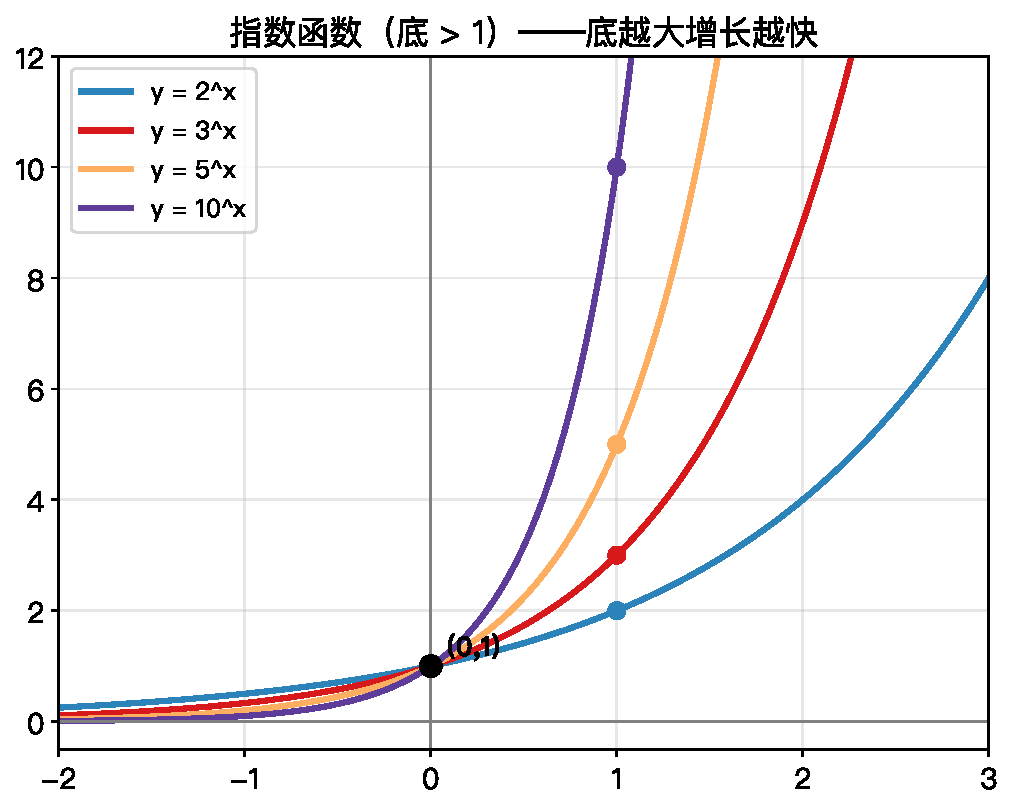
\includegraphics[width=0.6\textwidth]{figures/ch04_exponential_growth.pdf}
\end{center}

\textbf{观察规律：}
\begin{enumerate}
  \item 所有图像都经过 \((0,1)\)——因为 \(a^0 = 1\)
  \item 所有图像都经过 \((1,a)\)——因为 \(a^1 = a\)
  \item 底越大，增长越快（\(10^x\) 比 \(2^x\) 陡得多）
  \item 当 \(x < 0\) 时，函数值在 0 和 1 之间（如 \(2^{-1} = 0.5\)）
  \item 图像始终在 \(x\) 轴上方（\(a^x > 0\) 对所有实数 \(x\) 成立）
\end{enumerate}
\end{examplebox}

\begin{definitionbox}[指数函数的性质（底 > 1）]
\[
f(x) = a^x,\; a > 1
\]
\begin{itemize}
  \item \textbf{定义域}：\(\mathbb{R}\)（全体实数）
  \item \textbf{值域}：\((0, +\infty)\)（永远为正，但可以无限接近 0）
  \item \textbf{单调性}：严格递增（\(x_1 < x_2 \Rightarrow a^{x_1} < a^{x_2}\)）
  \item \textbf{水平渐近线}：\(y = 0\)（当 \(x \to -\infty\) 时，\(a^x \to 0\)）
  \item \textbf{经过点}：\((0,1)\)、\((1,a)\)
\end{itemize}
\end{definitionbox}


% ============================================================
\section{0 < 底 < 1：指数衰减}
% ============================================================

当底数在 0 和 1 之间时，函数值随着 \(x\) 增大而\textbf{逐渐衰减}。

\begin{examplebox}[3]
对比 \(y = (1/2)^x\)、\(y = (1/3)^x\)、\(y = (1/5)^x\)：

\begin{center}
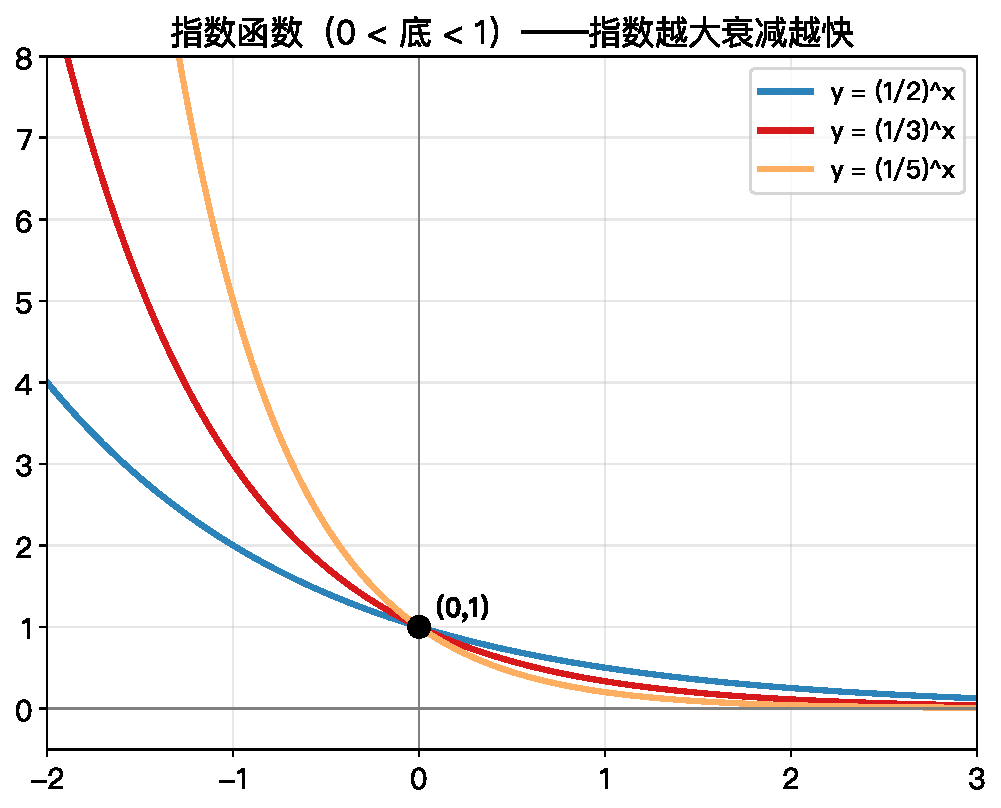
\includegraphics[width=0.6\textwidth]{figures/ch04_exponential_decay.pdf}
\end{center}

\textbf{观察规律：}
\begin{enumerate}
  \item 同样经过 \((0,1)\)
  \item 但这次是\textbf{递减}的——\(x\) 越大，函数值越小
  \item 底越小，衰减越快（\((1/5)^x\) 比 \((1/2)^x\) 下降得更快）
  \item 当 \(x \to +\infty\) 时，函数值趋近于 0
  \item 水平渐近线仍然是 \(y = 0\)
\end{enumerate}
\end{examplebox}


% ============================================================
\section{增长与衰减的对称关系}
% ============================================================

增长型 \(y = a^x\) 和衰减型 \(y = (1/a)^x\) 之间有优美的对称关系。

\begin{examplebox}[4]
\(y = 2^x\) 和 \(y = (1/2)^x\) 关于 \(y\) 轴对称：

\begin{center}
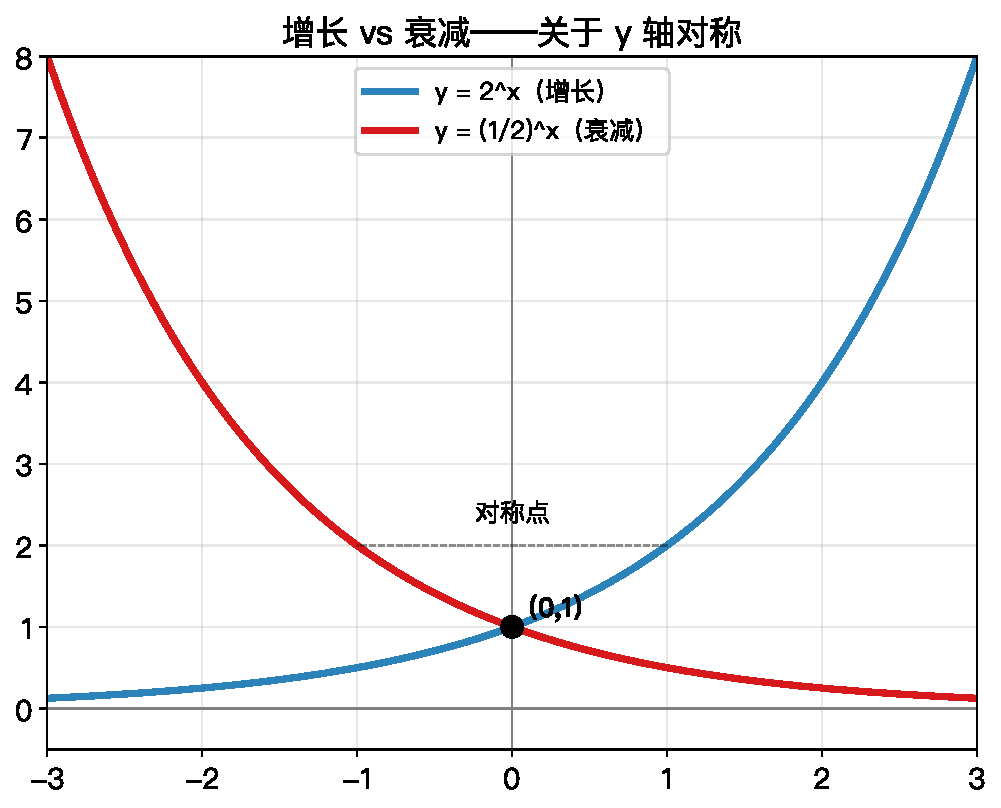
\includegraphics[width=0.6\textwidth]{figures/ch04_growth_vs_decay.pdf}
\end{center}

\textbf{原因：}
\[
\left(\frac{1}{2}\right)^x = (2^{-1})^x = 2^{-x}
\]

所以 \(y = (1/2)^x\) 其实就是 \(y = 2^{-x}\)——把 \(x\) 换成 \(-x\)，图像关于 \(y\) 轴对称。

\textbf{一般规律：}
\[
\boxed{a^x \text{ 和 } (1/a)^x \text{ 关于 } y \text{ 轴对称}}
\]
\end{examplebox}


% ============================================================
\section{自然指数 \(e^x\)——最重要的指数函数}
% ============================================================

在所有可能的底数中，有一个底数\textbf{特别重要}——它就是 \(e\)。

\begin{definitionbox}[自然常数 \(e\)]
\(e\) 是一个无理数，约等于 2.71828\ldots

它是自然对数的底数，也是数学中最重要的常数之一（和 \(\pi\) 齐名）。
\end{definitionbox}

\begin{examplebox}[5]
\(y = e^x\) 与 \(2^x\)、\(3^x\) 的对比：

\begin{center}
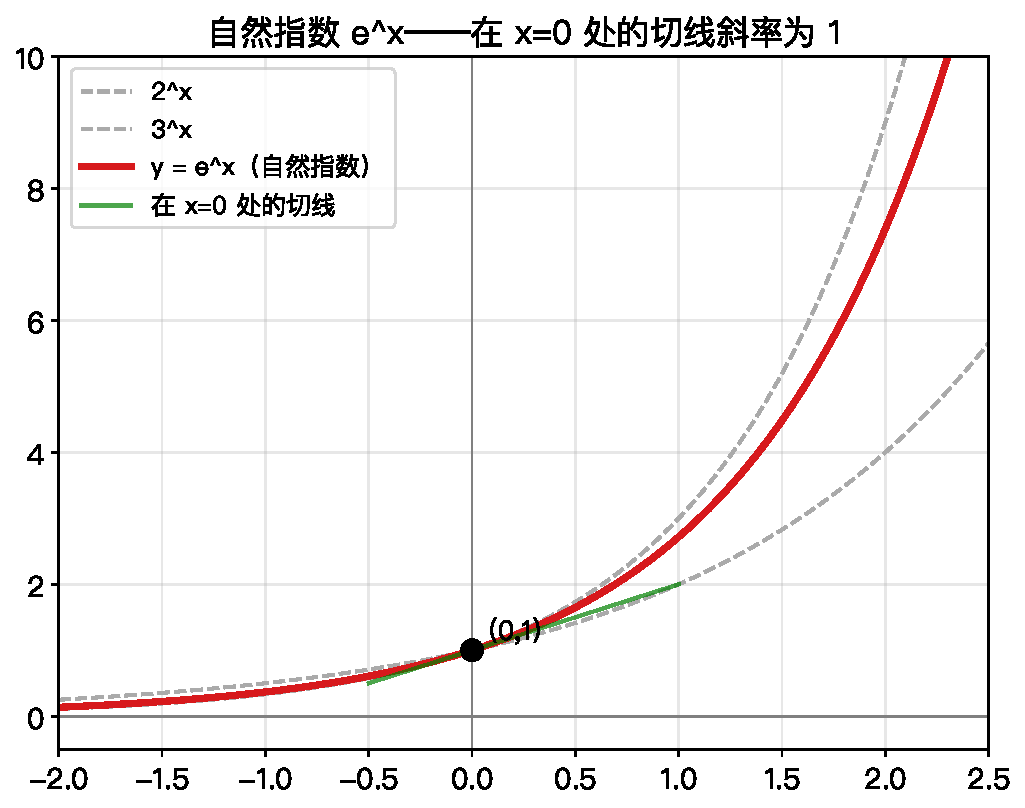
\includegraphics[width=0.6\textwidth]{figures/ch04_natural_exponential.pdf}
\end{center}

\textbf{为什么 \(e^x\) 这么重要？}
\begin{enumerate}
  \item 在 \(x=0\) 处，\(e^x\) 的切线斜率为 1（精确等于 1！）
  \item 这一点使得 \(e^x\) 的导数就是它自己（以后学导数时会详细讲）
  \item 自然界的很多现象都用 \(e^x\) 描述：人口增长、放射性衰变、复利计算
  \item AI 中 Softmax 的核心就是 \(e^x\)
\end{enumerate}
\end{examplebox}


% ============================================================
\section{指数函数 vs 幂函数——谁增长更快？}
% ============================================================

这是数学中一个\textbf{非常重要的结论}：

\begin{center}
\fcolorbox{red!50}{red!5}{\parbox{0.85\textwidth}{
\textbf{指数增长最终会超过任何幂函数增长。}\\
不管幂函数的指数多大（即使是 \(x^{100}\)），
总存在某个点之后，\textbf{指数函数永远大于幂函数}。
}}
\end{center}

\begin{examplebox}[6]
对比 \(2^x\)、\(x^2\)、\(x^3\)：

\begin{center}
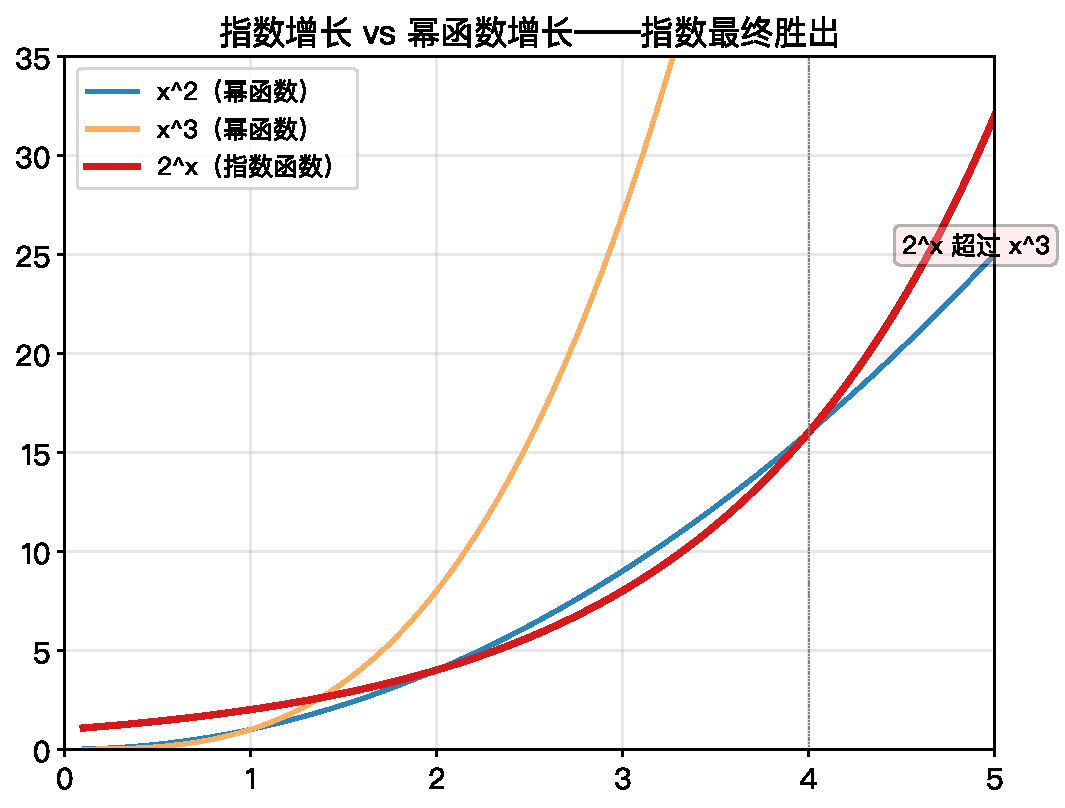
\includegraphics[width=0.6\textwidth]{figures/ch04_expo_vs_power.pdf}
\end{center}

\textbf{验证：}
\begin{center}
\begin{tabular}{c|c|c|c}
\(x\) & \(x^2\) & \(x^3\) & \(2^x\) \\
\hline
0 & 0 & 0 & 1 \\
1 & 1 & 1 & 2 \\
2 & 4 & 8 & 4 \\
3 & 9 & 27 & 8 \\
4 & 16 & 64 & 16 \\
5 & 25 & 125 & 32 \\
6 & 36 & 216 & 64 \\
7 & 49 & 343 & 128 \\
8 & 64 & 512 & 256 \\
9 & 81 & 729 & 512 \\
10 & 100 & 1000 & 1024 \\
\end{tabular}
\end{center}

在 \(x = 10\) 时，\(2^x = 1024\) 已经超过了 \(x^3 = 1000\)。
虽然 \(x^3\) 一开始领先，但指数函数\textbf{终究会超越}。
\end{examplebox}


% ============================================================
\section{指数方程}
% ============================================================

\begin{definitionbox}[指数方程]
指数里含有未知数的方程叫\textbf{指数方程}。

基本解法：将两边化为\textbf{同底}形式，然后让指数相等。
\[
a^{f(x)} = a^{g(x)} \quad\Longrightarrow\quad f(x) = g(x)
\]
\end{definitionbox}

\begin{examplebox}[7——解指数方程]
解方程：
\[
(1)\; 2^x = 8 \qquad (2)\; 3^{x+1} = 27 \qquad (3)\; 2^{2x-1} = 4^{x+3}
\]

解：
\[
\begin{aligned}
(1)&\; 2^x = 8 = 2^3 \;\Longrightarrow\; x = 3 \\
(2)&\; 3^{x+1} = 27 = 3^3 \;\Longrightarrow\; x+1 = 3 \;\Longrightarrow\; x = 2 \\
(3)&\; 2^{2x-1} = 4^{x+3} = (2^2)^{x+3} = 2^{2x+6} \\
    &\;\Longrightarrow\; 2x-1 = 2x+6 \;\Longrightarrow\; -1 = 6 \;\Longrightarrow\; \text{无解}
\end{aligned}
\]

\textbf{注意：} 第(3)题无解的原因是左右两边不可能相等。\\
\textbf{验证：} 左边 \(2^{2x-1}\)，右边 \(4^{x+3} = 2^{2x+6}\)，右边总是比左边大 \(2^7 = 128\) 倍。
\end{examplebox}

\begin{examplebox}[8——指数不等式]
解不等式 \(2^x > 8\)：

\[
2^x > 8 = 2^3 \;\Longrightarrow\; x > 3
\]

因为底数 \(2 > 1\)，指数函数递增，所以不等号方向不变。

如果底数在 0 和 1 之间，不等号会反向：
\[
\left(\frac{1}{2}\right)^x > \frac{1}{8} \;\Longrightarrow\; \left(\frac{1}{2}\right)^x > \left(\frac{1}{2}\right)^3 \;\Longrightarrow\; x < 3
\]
\end{examplebox}


% ============================================================
\section{指数函数在 AI 中的应用}
% ============================================================

\begin{examplebox}[9——Softmax 函数]
Softmax 是 AI 中最常用的函数之一，它将一组数转换成"概率"。

\[
\text{Softmax}(x_i) = \frac{e^{x_i}}{\sum_{j} e^{x_j}}
\]

\textbf{为什么用指数？}
\begin{enumerate}
  \item 指数保证输出为正数（概率不能为负）
  \item 指数放大了差距——输入的微小差异在输出中会被放大
  \item 所有输出的和为 1（满足概率的定义）
\end{enumerate}

\textbf{例：} 输入 \([2, 1, 0]\)：
\[
e^2 \approx 7.39,\quad e^1 \approx 2.72,\quad e^0 = 1
\]
\[
\text{Softmax} = \left[\frac{7.39}{7.39+2.72+1},\; \frac{2.72}{11.11},\; \frac{1}{11.11}\right] \approx [0.67, 0.24, 0.09]
\]

最大输入 2 被放大成了概率 67\%，这就是 Softmax 的"赢家通吃"效果。
\end{examplebox}


% ============================================================
\section{符号卡片}
% ============================================================

\begin{symbolcard}
\(a^x\) & \verb|a^x| & 读作"a 的 x 次方" & 指数函数，底 \(a\) 指数 \(x\) \\
\(e\) & \verb|e| & 读作"自然常数" & 约 2.71828，最重要的底数 \\
\(e^x\) & \verb|e^x| & 读作"e 的 x 次方" & 自然指数函数 \\
\((0, +\infty)\) & \verb|(0, +inf)| & 读作"0 到正无穷" & 指数函数的值域 \\
水平渐近线 & —— & —— & 指数函数当 \(x\to -\infty\) 时的极限 \\
\end{symbolcard}


% ============================================================
\section{代码验证}
% ============================================================

\begin{lstlisting}[caption=指数函数的数值验证]
import numpy as np

# 1. 验证指数函数经过 (0,1) 和 (1,a)
print("=== 指数函数经过 (0,1) ===")
for a in [2, 3, 5, 10]:
    print(f"  {a}^0 = {a**0},  {a}^1 = {a**1}")
print(f"  e^0 = {np.e**0},  e^1 = {np.e**1:.4f}")

print()

# 2. 指数增长 vs 幂函数增长
print("=== 指数 vs 幂函数（看谁大）===")
for x in range(0, 11):
    power2 = x**2
    power3 = x**3
    expo = 2**x
    winner = "指数!" if expo > power3 else ("幂函数" if power3 > expo else "打平")
    print(f"  x={x:2d}:  x^2={power2:4d},  x^3={power3:4d},  2^x={expo:5d}  <- {winner}")

print()

# 3. Softmax 模拟
def softmax(x):
    e_x = np.exp(x - np.max(x))  # 稳定版
    return e_x / np.sum(e_x)

scores = np.array([2.0, 1.0, 0.0])
probs = softmax(scores)
print("=== Softmax 示例 ===")
for i, (s, p) in enumerate(zip(scores, probs)):
    print(f"  输入 {s:.1f} -> 概率 {p:.3f} ({p*100:.1f}%)")
print(f"  概率和 = {np.sum(probs):.6f}")
\end{lstlisting}

运行结果：
\begin{lstlisting}[frame=none,backgroundcolor={},numbers=none]
=== 指数函数经过 (0,1) ===
  2^0 = 1,  2^1 = 2
  3^0 = 1,  3^1 = 3
  5^0 = 1,  5^1 = 5
  10^0 = 1,  10^1 = 10
  e^0 = 1,  e^1 = 2.7183

=== 指数 vs 幂函数（看谁大）===
  x= 0:  x^2=   0,  x^3=   0,  2^x=    1  <- 指数!
  x= 1:  x^2=   1,  x^3=   1,  2^x=    2  <- 指数!
  x= 2:  x^2=   4,  x^3=   8,  2^x=    4  <- 幂函数
  x= 3:  x^2=   9,  x^3=  27,  2^x=    8  <- 幂函数
  x= 4:  x^2=  16,  x^3=  64,  2^x=   16  <- 幂函数
  x= 5:  x^2=  25,  x^3= 125,  2^x=   32  <- 幂函数
  x= 6:  x^2=  36,  x^3= 216,  2^x=   64  <- 幂函数
  x= 7:  x^2=  49,  x^3= 343,  2^x=  128  <- 幂函数
  x= 8:  x^2=  64,  x^3= 512,  2^x=  256  <- 幂函数
  x= 9:  x^2=  81,  x^3= 729,  2^x=  512  <- 幂函数
  x=10:  x^2= 100,  x^3=1000,  2^x= 1024  <- 指数!

=== Softmax 示例 ===
  输入 2.0 -> 概率 0.665 (66.5%)
  输入 1.0 -> 概率 0.245 (24.5%)
  输入 0.0 -> 概率 0.090 (9.0%)
  概率和 = 1.000000
\end{lstlisting}


% ============================================================
\section{本章小结}
% ============================================================

\begin{progressbox}
\textbf{指数函数} \(y = a^x\)：底固定、指数变。所有指数函数经过 \((0,1)\) 和 \((1,a)\)。

\textbf{底 > 1}（增长型）：递增，底越大增长越快
\textbf{0 < 底 < 1}（衰减型）：递减，底越小衰减越快

\textbf{对称性}：\(a^x\) 和 \((1/a)^x\) 关于 \(y\) 轴对称

\textbf{自然指数} \(e^x\)：在 \(x=0\) 处切线斜率为 1，导数等于自己

\textbf{指数 vs 幂函数}：指数函数\textbf{最终胜出}——这是数学中最重要的增长对比

\textbf{AI 应用}：Softmax 用指数把输入转换成概率，放大差距
\end{progressbox}

\subsection*{通往下一章}

\textbf{这一章}你学会了指数函数——增长的终极武器。

\textbf{下一章}我们学\textbf{对数函数}——指数的"逆运算"。
如果说指数回答的是"给定底数和指数，结果是多少"，对数回答的就是\,"给定底数和结果，指数是多少"。
这两个函数是数学中最重要的"搭档"。


% ============================================================
% 习题
% ============================================================
\section{习题}

% ===== 送分 =====

\begin{exercise}[0]
判断是指数函数还是幂函数：
\[
(1)\; y = 4^x \quad (2)\; y = x^4 \quad (3)\; y = \pi^x \quad (4)\; y = x^{\pi}
\]
\GoodExercise{exp-vs-power}
\end{exercise}

\begin{exercise}[0]
计算：
\[
(1)\; 2^3 \quad (2)\; 2^0 \quad (3)\; 2^{-2} \quad (4)\; 4^{1/2}
\]
\end{exercise}

\begin{exercise}[0]
指数函数 \(y = 3^x\) 经过哪两个固定点？
\end{exercise}

\begin{exercise}[0]
比较大小（不用计算器）：
\[
(1)\; 2^3 \text{ 和 } 3^2 \qquad
(2)\; 2^{-1} \text{ 和 } 2^0
\]
\end{exercise}

% ===== 简单 =====

\begin{exercise}[1]
画出 \(y = 2^x\) 的草图（取 \(x = -2, -1, 0, 1, 2\) 五个点），标出关键点坐标。
\end{exercise}

\begin{exercise}[1]
判断 \(y = 3^x\) 是递增还是递减？\(y = (1/3)^x\) 呢？
\end{exercise}

\begin{exercise}[1]
计算：
\[
(1)\; 2^3 \times 2^4 \qquad (2)\; \frac{3^5}{3^2} \qquad (3)\; (2^2)^3
\]
\end{exercise}

\begin{exercise}[1]
填空：当 \(x\) 很大时，\(2^x\) 的值趋近于\_\_\_\_；当 \(x\) 很负时，\(2^x\) 的值趋近于\_\_\_\_。
\end{exercise}

% ===== 基础 =====

\begin{exercise}[2]
在同一坐标系中画出 \(y = 2^x\) 和 \(y = (1/2)^x\) 的草图，它们是什么关系？
\end{exercise}

\begin{exercise}[2]
解方程：
\[
(1)\; 2^x = 16 \qquad (2)\; 3^{x-1} = 27 \qquad (3)\; 5^{2x} = 25
\]
\end{exercise}

\begin{exercise}[2]
比较大小：
\[
(1)\; 2^{0.5} \text{ 和 } 2^{0.8} \qquad
(2)\; (0.5)^{0.5} \text{ 和 } (0.5)^{0.8} \qquad
\]
（提示：注意底数是否大于 1）
\end{exercise}

\begin{exercise}[2]
一种细菌每 30 分钟分裂一次（数量翻倍）。开始时只有 1 个细菌，\(t\) 小时后有多少个？
写出表达式。
\end{exercise}

% ===== 普通 =====

\begin{exercise}[3]
已知 \(f(x) = 2^x\)，求：
\[
f(0),\; f(1),\; f(-2),\; f(a),\; f(a+1)
\]
\end{exercise}

\begin{exercise}[3]
解不等式：
\[
(1)\; 2^x > 32 \qquad (2)\; 3^{x-1} \le 9 \qquad (3)\; (1/2)^x > 1/8
\]
\end{exercise}

\begin{exercise}[3]
\(y = 2^x + 1\) 的图像是由 \(y = 2^x\) 经过什么变换得到的？它的水平渐近线是什么？
\end{exercise}

\begin{exercise}[3]
比较 \(2^x\) 和 \(x^2\) 的大小关系（取 \(x = 1, 2, 3, 4, 5\) 分别计算并比较）。
\end{exercise}

\begin{exercise}[3]
某种放射性物质每年衰减 5\%（即每年剩余为上一年的 95\%）。初始质量为 100 克。
\begin{enumerate}
  \item[(1)] 写出 \(t\) 年后的质量表达式
  \item[(2)] 求 10 年后的剩余质量（保留整数）
\end{enumerate}
\end{exercise}

% ===== 中等 =====

\begin{exercise}[4]
解方程：
\[
(1)\; 2^{x+1} = 4^{x-1} \qquad (2)\; 3^{2x} - 3^x - 6 = 0
\]
（提示：(2) 令 \(t = 3^x\)，化为关于 \(t\) 的二次方程）
\end{exercise}

\begin{exercise}[4]
已知 \(f(x) = a^x\) 经过点 \((2, 9)\)，求 \(a\) 的值，并写出 \(f(x)\) 的表达式。
\end{exercise}

\begin{exercise}[4]
\(y = 3^{x-2} + 1\) 是由 \(y = 3^x\) 经过怎样的平移得到的？
它的值域和水平渐近线是什么？
\end{exercise}

\begin{exercise}[4]
某城市人口每年增长 2\%。现在有 100 万人，多少年后人口翻倍？
（提示：解 \(100 \times 1.02^t = 200\)，尝试 \(t = 35\) 和 \(t = 36\) 看看哪个接近）
\end{exercise}

\begin{exercise}[4]
对于 \(y = a^x\)（\(a > 0, a \neq 1\)），证明：
\[
f(x) \cdot f(y) = f(x + y)
\]
并用这个性质计算 \(2^3 \times 2^4\)。
\end{exercise}

% ===== 进阶 =====

\begin{exercise}[5]
解方程 \(4^x - 2^{x+1} - 8 = 0\)。
（提示：\(4^x = (2^2)^x = 2^{2x} = (2^x)^2\)，令 \(t = 2^x\)）
\end{exercise}

\begin{exercise}[5]
已知函数 \(f(x) = 2^x - 2^{-x}\)。
\begin{enumerate}
  \item[(1)] 判断 \(f(x)\) 的奇偶性
  \item[(2)] 证明 \(f(x)\) 是递增函数
\end{enumerate}
\end{exercise}

\begin{exercise}[5]
某种药物的血药浓度随时间变化为 \(C(t) = C_0 \cdot e^{-kt}\)。
已知初始浓度 \(C_0 = 100\)，2 小时后浓度降为 50。
\begin{enumerate}
  \item[(1)] 求 \(k\) 的值
  \item[(2)] 4 小时后的浓度是多少？
\end{enumerate}
\end{exercise}

\begin{exercise}[5]
比较 \(2^{\pi}\) 和 \(\pi^2\) 的大小（提示：\(2^\pi\) 是指数，\(\pi^2\) 是幂函数）。
\end{exercise}

% ===== 拔高 =====

\begin{exercise}[6]
已知 \(f(x) = \dfrac{e^x - e^{-x}}{2}\)（这个函数叫双曲正弦，以后会学到）。
\begin{enumerate}
  \item[(1)] 证明 \(f\) 是奇函数
  \item[(2)] 证明 \(f\) 是递增函数
  \item[(3)] 解方程 \(f(x) = 1\)（提示：令 \(t = e^x\)）
\end{enumerate}
\end{exercise}

\begin{exercise}[6]
对于指数函数 \(f(x) = a^x\)（\(a > 1\)），证明：
\[
\frac{f(x_1) + f(x_2)}{2} \ge f\left(\frac{x_1 + x_2}{2}\right)
\]
这个性质叫\textbf{指数函数的凸性}——图像始终在弦的下方（以后学导数时会用这个性质）。
\end{exercise}

\begin{exercise}[6]
已知 \(a > 0, a \neq 1\)，\(f(x) = a^{x} + a^{-x}\)。
\begin{enumerate}
  \item[(1)] 判断奇偶性
  \item[(2)] 求最小值（提示：利用 \(a^x + a^{-x} \ge 2\) 的基本不等式）
\end{enumerate}
\end{exercise}

% ===== 极难 =====

\begin{exercise}[7]
已知 \(f(x) = 2^x\)，\(g(x) = x^2\)。
\begin{enumerate}
  \item[(1)] 列出 \(x = 1, 2, 3, 4, 5, 10, 20\) 时 \(f(x)\) 和 \(g(x)\) 的值
  \item[(2)] 证明：存在一个 \(N\)，使得对所有 \(x > N\)，有 \(2^x > x^2\)
  \item[(3)] 找到最小的整数 \(N\) 满足这个性质
\end{enumerate}

\textbf{说明：} 这道题让你亲手验证"指数函数最终超过幂函数"这个重要结论。
找到那个"转折点"N 是数学分析中常见的思维方式。
\end{exercise}

% ============================================================
% 第5章：对数函数——指数的逆运算
% ============================================================

\chapter{对数函数——指数的逆运算}

\begin{applicationbox}
\textbf{学完本章你能做什么？}
\begin{enumerate}
  \item \textbf{学之前}：你学会了指数函数 \(2^x = 8\) 可以解出 \(x=3\)，但如果 \(2^x = 10\) 呢？
  \item \textbf{学之后}：你会用对数来解这类问题——"指数是多少"。你还会理解 AI 中交叉熵损失函数为什么离不开对数。
  \item \textbf{日常例子}：地震的里氏震级是对数尺度的——震级每增加 1，能量释放增加约 32 倍。
        声音的分贝也是对数尺度。对数把"天文数字"压缩成好理解的小数字。
\end{enumerate}
\end{applicationbox}


% ============================================================
\section{从第4章来——指数函数的"逆问题"}
% ============================================================

第4章我们学了指数函数 \(f(x) = a^x\)——给定底 \(a\) 和指数 \(x\)，求值 \(a^x\)。

现在问一个相反的问题：

\begin{center}
\fcolorbox{blue!40}{blue!5}{\parbox{0.8\textwidth}{
\textbf{已知底数和结果，求指数：} \\
\(2^? = 8\) —— 答案显然是 \(3\)（因为 \(2^3 = 8\)）。\\
但 \(2^? = 10\) 呢？指数是多少？
}}
\end{center}

这个问题就是\textbf{对数}要解决的。

\begin{examplebox}[1——补全对数表  🔓 完全展开]
补全下表（你能看出规律吗？）：

\begin{center}
\begin{tabular}{c|c|c|c|c|c}
\(x\) & -2 & -1 & 0 & 1 & 2 \\
\hline
\(2^x\) & 1/4 & 1/2 & 1 & 2 & 4 \\
反过来：\(? = \log_2(\text{结果})\) & \(\log_2(1/4)\) & \(\log_2(1/2)\) & \(\log_2(1)\) & \(\log_2(2)\) & \(\log_2(4)\) \\
\hline
这个"反过来的指数"等于 & -2 & -1 & 0 & 1 & 2 \\
\end{tabular}
\end{center}

\textbf{规律：} 对数 \(\log_2(y)\) 回答的是"2 的几次方等于 \(y\)"。
\textbf{为什么？} 因为对数就是指数。表格中 \(2^x\) 那一行给出的是指数运算的结果，
底下的"反过来的指数"就是底数 2 到那个结果需要的指数——也就是 \(\log_2(y)\)。
\end{examplebox}


% ============================================================
\section{对数的定义}
% ============================================================

\begin{definitionbox}[对数]
如果 \(a > 0\) 且 \(a \neq 1\)，那么
\[
a^b = c \quad\Longleftrightarrow\quad \log_a c = b
\]
读作：\textbf{以 \(a\) 为底的 \(c\) 的对数等于 \(b\)}。

其中：
\begin{itemize}
  \item \(a\) 是\textbf{底数}（base）
  \item \(c\) 是\textbf{真数}（读作 zhēn shù，必须大于 0）
  \item \(b\) 是\textbf{对数}（logarithm）
\end{itemize}
\end{definitionbox}

\begin{examplebox}[2——指数式与对数式的互化  🔒₁ 请完成最后一行]
\begin{center}
\begin{tabular}{c|c}
\textbf{指数式} & \textbf{对数式} \\
\hline
\(2^3 = 8\) & \(\log_2 8 = 3\) \\
\(3^2 = 9\) & \(\log_3 9 = 2\) \\
\(5^{-1} = 1/5\) & \(\log_5 (1/5) = -1\) \\
\(10^0 = 1\) & \(\log_{10} 1 = 0\) \\
\hline
\(a^b = c\) & \multicolumn{1}{c}{\textbf{请你写出来：}}
\end{tabular}
\end{center}

\textbf{记忆：}对数 = 指数。\(\log_a c\) 就是"把 \(a\) 变成 \(c\) 所需要的指数"。
\end{examplebox}


% ============================================================
\section{常用对数与自然对数}
% ============================================================

\begin{definitionbox}[两种最重要的对数]
\begin{enumerate}
  \item \textbf{常用对数}：底为 10，记作 \(\lg x = \log_{10} x\)。
        用于科学计算、地震震级、声音分贝。
  \item \textbf{自然对数}：底为 \(e\)，记作 \(\ln x = \log_e x\)。
        用于数学分析、AI、物理、生物学。
\end{enumerate}
\end{definitionbox}

\begin{examplebox}[3——记住几个关键值  🔒₂ 请完成最后两个]
\begin{align*}
  \lg 1 &= 0 \quad &\text{（因为 } 10^0 = 1\text{）} \\
  \lg 10 &= 1 \quad &\text{（因为 } 10^1 = 10\text{）} \\
  \lg 100 &= 2 \quad &\text{（因为 } 10^2 = 100\text{）} \\
  \\
  \ln 1 &= \quad &\text{请你写：} \\
  \ln e &= \quad &\text{请你写：}
\end{align*}
\end{examplebox}


% ============================================================
\section{对数的运算法则}
% ============================================================

\begin{theorembox}[对数运算法则]
设 \(a > 0, a \neq 1\)，\(M > 0, N > 0\)：
\begin{align*}
  \log_a (MN) &= \log_a M + \log_a N \quad &\text{（乘变加）} \\
  \log_a \frac{M}{N} &= \log_a M - \log_a N \quad &\text{（除变减）} \\
  \log_a M^n &= n \log_a M \quad &\text{（指数变系数）} \\
  \log_a \sqrt[n]{M} &= \frac{1}{n} \log_a M \quad &\text{（根号变分数）}
\end{align*}
\end{theorembox}

\begin{notebox}
\textbf{记忆口诀：}\\
乘变加，除变减，指数变系数，根号变分数。
\end{notebox}

\begin{examplebox}[4——对数运算  🔒₃ 只给开头，你来完成]
计算：
\[
(1)\; \lg 2 + \lg 5 \qquad (2)\; \log_2 8 - \log_2 2 \qquad (3)\; \log_3 9^2
\]

\textbf{给你一个开头：}
\[
(1)\; \lg 2 + \lg 5 = \lg(2 \times 5) = \lg 10 = 1
\]

\textbf{你来完成 (2) 和 (3)：} 使用对数运算法则（乘变加、除变减、指数变系数）。
写出每一步的依据。完成后用下面方法验算：
\[
\log_3 81 = ? \quad (\text{因为 } 3^? = 81)
\]
\end{examplebox}

% ── 信心校准（渐退序列中段）──
\begin{confidencebox}
从例1（完全展开）到例4（只给开头），你感觉到难度递增了吗？
如果例4卡住了，说明对数运算法则还不够熟——回看本节定理框，把"乘变加、除变减、指数变系数"默写一遍。
\end{confidencebox}


\begin{examplebox}[5——换底公式]
\textbf{换底公式}（重要）：
\[
\log_a b = \frac{\log_c b}{\log_c a}
\]

特别地：\(\log_a b = \frac{\ln b}{\ln a} = \frac{\lg b}{\lg a}\)

\textbf{例：} 计算 \(\log_2 5\)（用计算器算 \(\ln 5\) 和 \(\ln 2\)）：
\[
\log_2 5 = \frac{\ln 5}{\ln 2} \approx \frac{1.6094}{0.6931} \approx 2.3219
\]

验证：\(2^{2.3219} \approx 5\) [OK]
\end{examplebox}


% ============================================================
\section{对数函数 \(y = \log_a x\)}
% ============================================================

\begin{definitionbox}[对数函数]
形如
\[
f(x) = \log_a x \quad (a > 0,\; a \neq 1,\; x > 0)
\]
的函数称为\textbf{对数函数}（读作 duì shù hán shù，英文 logarithmic function）。

它是\textbf{指数函数 \(a^x\) 的反函数}。
\end{definitionbox}

\subsection{底 > 1：增长型对数函数}

\begin{examplebox}[6]
对比 \(y = \log_2 x\)、\(y = \ln x\)、\(y = \lg x\)：

\begin{center}
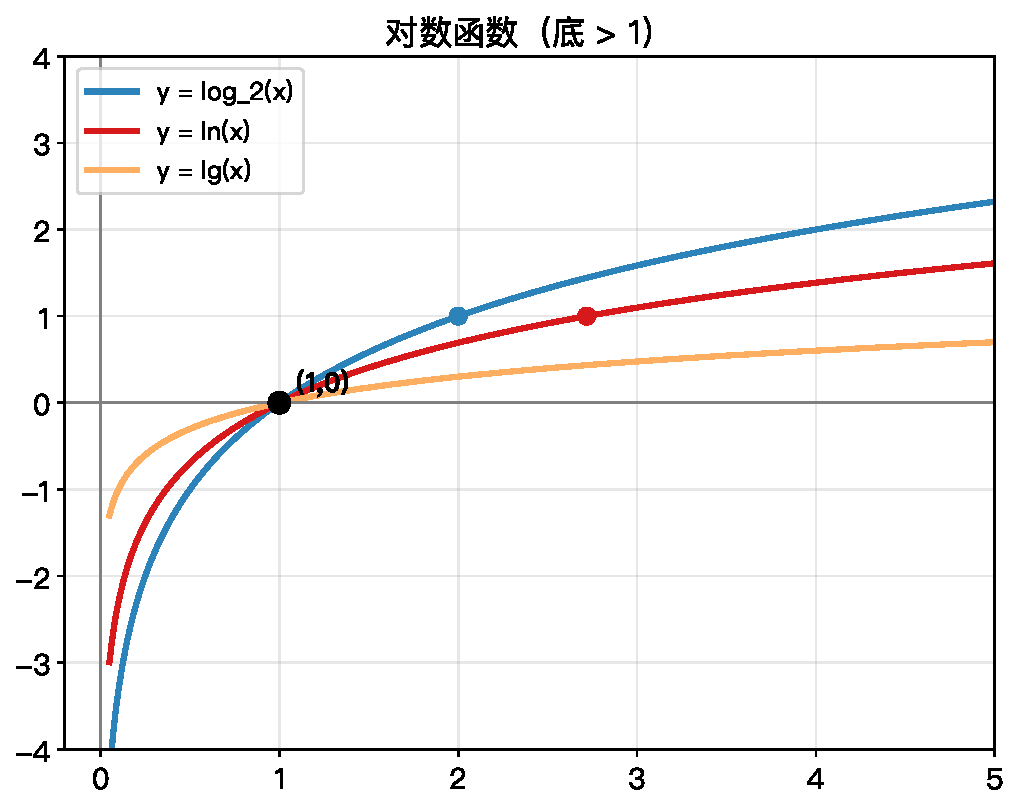
\includegraphics[width=0.6\textwidth]{figures/ch05_logarithm_bases.pdf}
\end{center}

\textbf{观察规律：}
\begin{enumerate}
  \item 所有对数函数都经过 \((1,0)\)——因为 \(\log_a 1 = 0\)
  \item 所有对数函数都经过 \((a,1)\)——因为 \(\log_a a = 1\)
  \item 底越大，增长越\textbf{慢}（\(\log_2 x\) 比 \(\lg x\) 增长快）
  \item 定义域：\(x > 0\)（负数没有对数）
  \item 值域：\(\mathbb{R}\)（全体实数）
  \item 垂直渐近线：\(x = 0\)（当 \(x \to 0^+\) 时，\(\log_a x \to -\infty\)）
\end{enumerate}
\end{examplebox}

\subsection{0 < 底 < 1：衰减型对数函数}

\begin{examplebox}[7]
\begin{center}
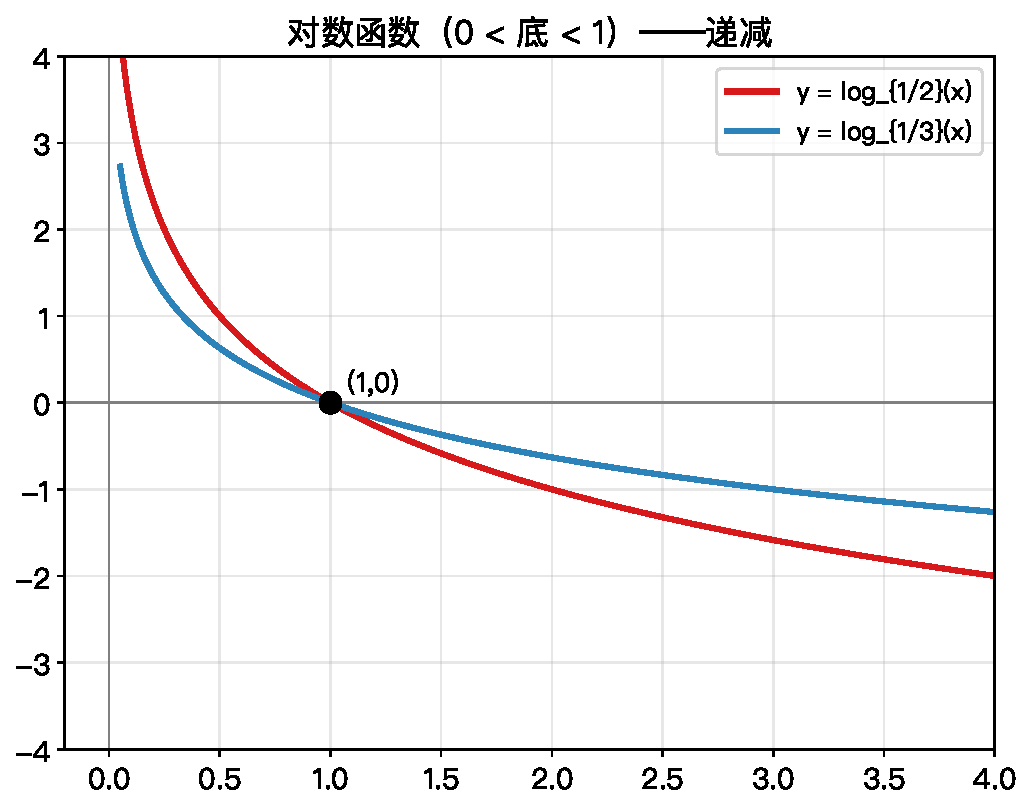
\includegraphics[width=0.6\textwidth]{figures/ch05_logarithm_decay.pdf}
\end{center}

\textbf{对比底>1：}
\begin{itemize}
  \item 还是经过 \((1,0)\)——但现在是\textbf{递减}的
  \item 底越小，衰减越快
  \item 当 \(x \to 0^+\) 时，\(\log_a x \to +\infty\)（与底>1相反）
\end{itemize}
\end{examplebox}


% ============================================================
\section{指数与对数——互逆关系}
% ============================================================

指数函数和对数函数是\textbf{互为反函数}的关系。

\begin{theorembox}[指数与对数的互逆]
如果 \(f(x) = a^x\)，那么它的反函数是 \(f^{-1}(x) = \log_a x\)。

两者的图像关于直线 \(y = x\) 对称：
\[
(a^x \text{ 上的点 } (b, a^b)) \;\longleftrightarrow\; (\log_a x \text{ 上的点 } (a^b, b))
\]
\end{theorembox}

\begin{examplebox}[8]
\(y = 2^x\) 和 \(y = \log_2 x\) 关于 \(y = x\) 对称：

\begin{center}
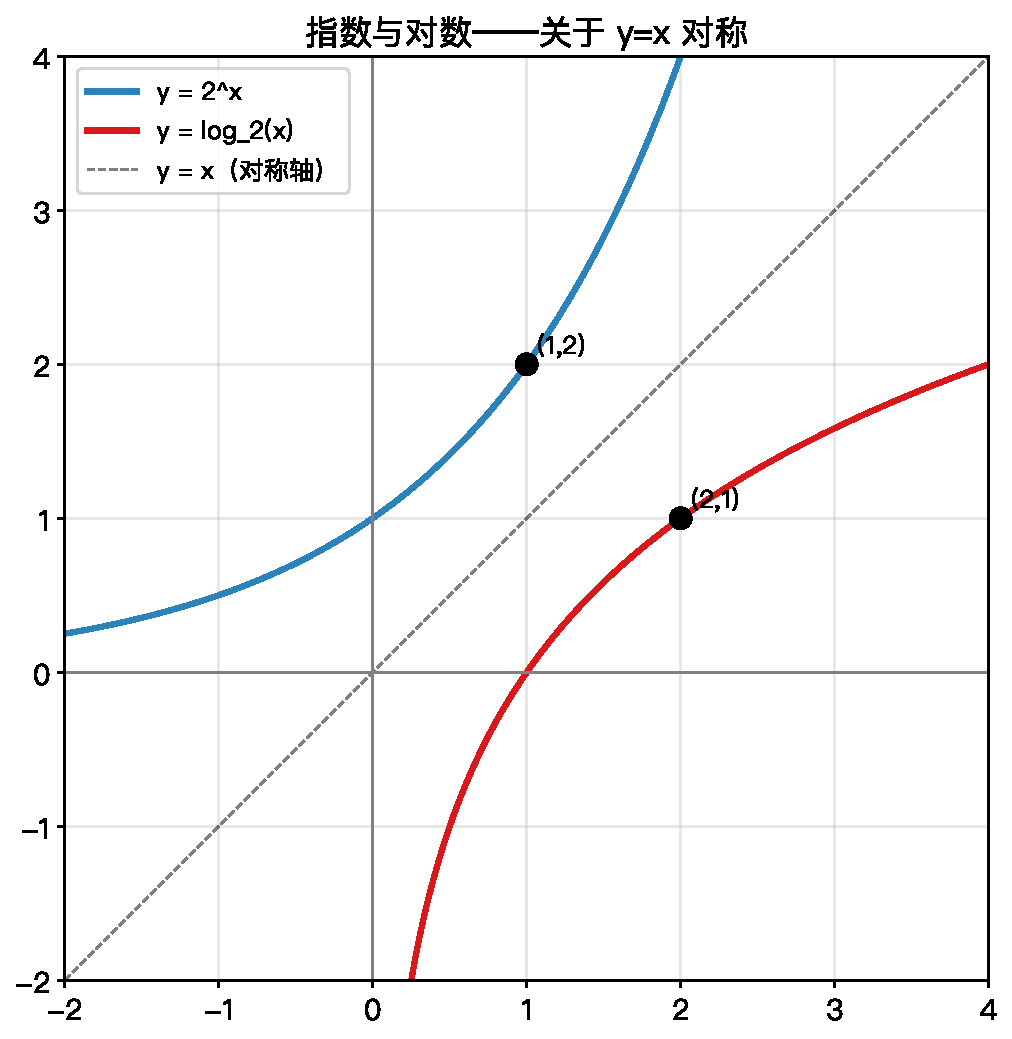
\includegraphics[width=0.55\textwidth]{figures/ch05_exp_log_inverse.pdf}
\end{center}

\textbf{具体验证：}
\[
2^3 = 8 \;\Longrightarrow\; (3, 8) \text{ 在 } y=2^x \text{ 上}
\]
\[
\log_2 8 = 3 \;\Longrightarrow\; (8, 3) \text{ 在 } y=\log_2 x \text{ 上}
\]

两个点的坐标互换了位置——这就是\textbf{反函数}的本质。
\end{examplebox}


% ============================================================
\section{对数的"压缩"效果}
% ============================================================

对数有一个重要的实际作用——\textbf{把大数压缩成小数}。

\begin{examplebox}[9]
\begin{center}
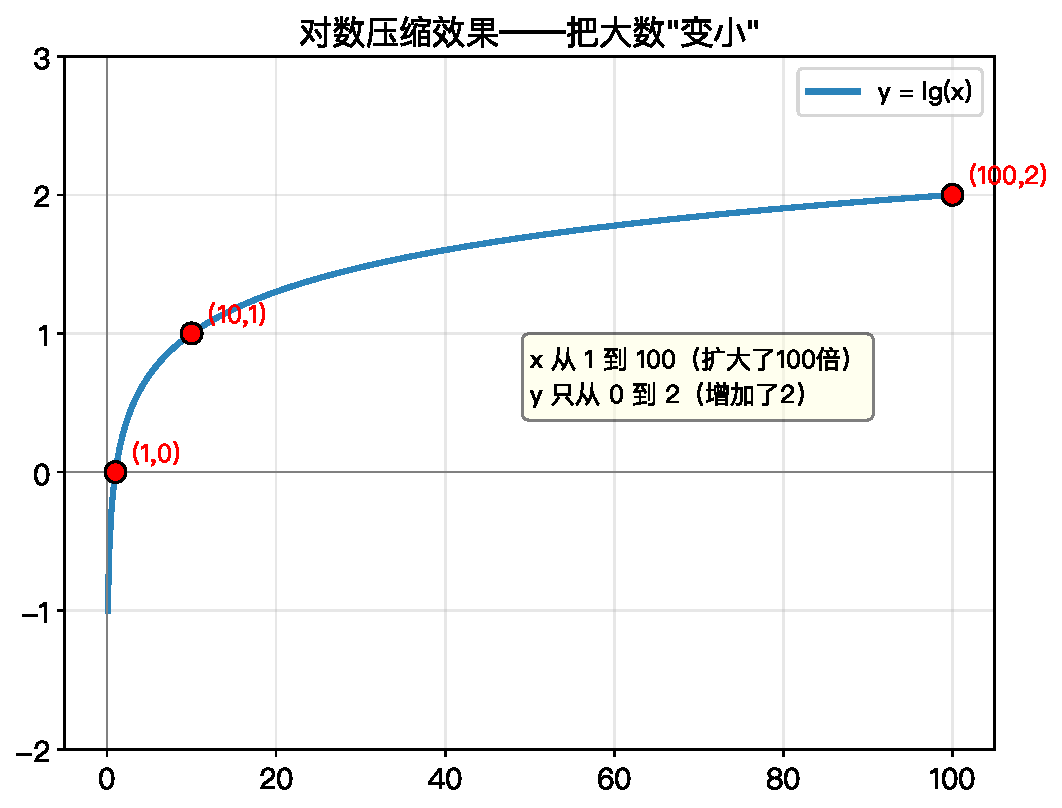
\includegraphics[width=0.55\textwidth]{figures/ch05_log_compression.pdf}
\end{center}

\textbf{看这个表：}
\begin{center}
\begin{tabular}{c|c}
\(x\) & \(\lg x\) \\
\hline
1 & 0 \\
10 & 1 \\
100 & 2 \\
1000 & 3 \\
1,000,000 & 6 \\
1,000,000,000 & 9 \\
\end{tabular}
\end{center}

\(x\) 从 1 扩大到 10 亿（扩大了 10 亿倍），\(\lg x\) 只从 0 增加到 9（增加了 9）。\\
这就是\textbf{对数压缩}——把天文数字变成好处理的小数字。

\textbf{应用：}地震震级（里氏 6 级比 5 级能量大约 32 倍）、声音分贝、pH 值、AI 中的交叉熵。
\end{examplebox}


% ============================================================
\section{对数方程与不等式}
% ============================================================

\begin{definitionbox}[对数方程]
真数中含有未知数的方程叫\textbf{对数方程}。

解法：利用对数的定义和运算法则，转化为普通方程。

\textbf{注意：}解出来之后一定要\textbf{验根}——真数必须大于 0！
\end{definitionbox}

\begin{examplebox}[10——解对数方程]
解方程：
\[
(1)\; \log_2 x = 3 \qquad (2)\; \lg(x+1) + \lg(x-1) = \lg 3
\]

解：
\[
\begin{aligned}
(1)&\; \log_2 x = 3 \;\Longrightarrow\; x = 2^3 = 8 \\
   &\;\text{验根：} x = 8 > 0 \;\text{[OK]}
\end{aligned}
\]

\[
\begin{aligned}
(2)&\; \lg(x+1) + \lg(x-1) = \lg 3 \\
   &\;\lg[(x+1)(x-1)] = \lg 3 \\
   &\;(x+1)(x-1) = 3 \\
   &\;x^2 - 1 = 3 \;\Longrightarrow\; x^2 = 4 \;\Longrightarrow\; x = \pm 2 \\
   &\;\text{验根：} x = 2 \text{ 时，} x+1 > 0,\; x-1 > 0 \;\text{[OK]} \\
   &\;\text{验根：} x = -2 \text{ 时，} x-1 = -3 < 0 \;\text{（真数不能为负）[X]} \\
   &\;\text{所以 } x = 2 \text{ 是唯一解。}
\end{aligned}
\]
\end{examplebox}


% ============================================================
\section{对数在 AI 中的应用——交叉熵损失}
% ============================================================

\begin{examplebox}[11——交叉熵损失函数]
在 AI 分类任务中，模型输出一个概率分布，我们需要衡量"预测分布"和"真实分布"的差距。

\[
\text{Loss} = -\sum_{i} y_i \log(p_i)
\]

其中 \(y_i\) 是真实标签（0 或 1），\(p_i\) 是模型预测的概率。

\textbf{为什么用对数？}
\begin{enumerate}
  \item 当 \(p_i\) 接近 1（预测正确）时，\(\log(p_i) \approx 0\)，loss 很小
  \item 当 \(p_i\) 接近 0（预测错误）时，\(\log(p_i) \to -\infty\)，loss 很大
  \item 对数放大了"错误预测"的惩罚——模型会拼命避免犯错
\end{enumerate}

\textbf{例：} 真实标签 \(y = [1, 0, 0]\)，预测 \(p = [0.8, 0.15, 0.05]\)：
\[
\text{Loss} = -(1\cdot\ln 0.8 + 0\cdot\ln 0.15 + 0\cdot\ln 0.05) = -\ln 0.8 \approx 0.223
\]
\end{examplebox}


% ============================================================
\section{符号卡片}
% ============================================================

\begin{symbolcard}
\(\log_a c\) & \verb|\log_a c| & 读作"以 a 为底 c 的对数" & \(a\) 的几次方等于 \(c\) \\
\(\lg x\) & \verb|\lg x| & 读作"常用对数 x" & \(\log_{10} x\)，底为 10 \\
\(\ln x\) & \verb|\ln x| & 读作"自然对数 x" & \(\log_e x\)，底为 \(e\) \\
真数 & —— & 读作"zhēn shù" & 对数中的 \(c\)，必须 \(> 0\) \\
\end{symbolcard}


% ============================================================
\section{代码验证}
% ============================================================

\begin{lstlisting}[caption=对数函数的数值验证]
import numpy as np

# 1. 验证指数和对数的互逆关系
print("=== 指数与对数互逆 ===")
for x in [1, 2, 3, 4, 5]:
    exp_val = 2**x
    log_val = np.log2(exp_val)
    print(f"  2^{x} = {exp_val:3d},  log2({exp_val:3d}) = {log_val}")

print()

# 2. 验证对数运算法则
print("=== 对数运算法则 ===")
print(f"  lg(2) + lg(5) = {np.log10(2) + np.log10(5):.4f}")
print(f"  lg(10)       = {np.log10(10):.4f}")
print(f"  log2(8*4)    = {np.log2(8*4):.4f}  (应等于 log2(8)+log2(4) = {np.log2(8)+np.log2(4):.4f})")

print()

# 3. 交叉熵损失模拟
def cross_entropy(y_true, y_pred):
    """计算交叉熵损失"""
    # 防止 log(0)
    eps = 1e-15
    y_pred = np.clip(y_pred, eps, 1 - eps)
    return -np.sum(y_true * np.log(y_pred))

print("=== 交叉熵损失 ===")
y_true = np.array([1, 0, 0])
good_pred = np.array([0.95, 0.03, 0.02])
bad_pred = np.array([0.3, 0.4, 0.3])
print(f"  正确预测的损失: {cross_entropy(y_true, good_pred):.4f}")
print(f"  错误预测的损失: {cross_entropy(y_true, bad_pred):.4f}")
print(f"  完美预测的损失: {cross_entropy(y_true, np.array([1, 0, 0])):.4f}")
\end{lstlisting}

运行结果：
\begin{lstlisting}[frame=none,backgroundcolor={},numbers=none]
=== 指数与对数互逆 ===
  2^1 =   2,  log2(  2) = 1.0
  2^2 =   4,  log2(  4) = 2.0
  2^3 =   8,  log2(  8) = 3.0
  2^4 =  16,  log2( 16) = 4.0
  2^5 =  32,  log2( 32) = 5.0

=== 对数运算法则 ===
  lg(2) + lg(5) = 1.0000
  lg(10)       = 1.0000
  log2(8*4)    = 5.0000  (应等于 log2(8)+log2(4) = 5.0000)

=== 交叉熵损失 ===
  正确预测的损失: 0.0513
  错误预测的损失: 1.2040
  完美预测的损失: 0.0000
\end{lstlisting}


% ============================================================
\section{本章小结}
% ============================================================

\begin{progressbox}
\textbf{对数的定义}：\(a^b = c \;\Longleftrightarrow\; \log_a c = b\)——对数就是指数。

\textbf{运算法则}：乘变加、除变减、指数变系数

\textbf{对数函数} \(y = \log_a x\)：
\begin{itemize}
  \item 定义域 \(x > 0\)，值域 \(\mathbb{R}\)，经过 \((1,0)\) 和 \((a,1)\)
  \item 底 > 1：递增；0 < 底 < 1：递减
  \item 垂直渐近线 \(x = 0\)
\end{itemize}

\textbf{指数与对数互逆}：\(y = a^x\) 和 \(y = \log_a x\) 关于 \(y = x\) 对称

\textbf{对数压缩}：把天文数字变成小数字——地震震级、分贝、交叉熵

\textbf{AI 应用}：交叉熵损失函数用对数放大错误惩罚
\end{progressbox}

\subsection*{通往下一章}

\textbf{这一章}你学会了对数函数——指数的逆运算。

\textbf{下一章}我们将进入\textbf{三角函数}——描述周期运动的数学工具。
从声音的波形到地球绕太阳公转，再到 AI 中的位置编码（Transformer），
三角函数无处不在。


% ============================================================
% 习题
% ============================================================
\section{习题}

% ===== 送分 =====

\begin{exercise}[0]
将指数式化为对数式：
\[
(1)\; 2^4 = 16 \qquad (2)\; 3^3 = 27 \qquad (3)\; 10^2 = 100
\]
\end{exercise}

\begin{exercise}[0]
将对数式化为指数式：
\[
(1)\; \log_2 8 = 3 \qquad (2)\; \log_3 81 = 4 \qquad (3)\; \lg 1000 = 3
\]
\end{exercise}

\begin{exercise}[0]
求值：
\[
(1)\; \lg 10 \qquad (2)\; \ln e \qquad (3)\; \log_5 25 \qquad (4)\; \log_2 1
\]
\end{exercise}
\qquad \textcolor{gray}{[回顾第4章：指数与对数的互逆]}%

\begin{exercise}[0]
判断正误：
\[
(1)\; \lg 100 = 2 \qquad (2)\; \ln 1 = 1 \qquad (3)\; \log_3 9 = 2 \qquad (4)\; \log_2 0 = 0
\]

% ===== 简单 =====

\end{exercise}

\begin{exercise}[1]
用 \(\lg 2\) 和 \(\lg 3\) 表示：
\[
(1)\; \lg 6 \qquad (2)\; \lg \frac{2}{3} \qquad (3)\; \lg 8
\]
\end{exercise}

\begin{exercise}[1]
计算：
\[
(1)\; \lg 20 - \lg 2 \qquad (2)\; \log_3 5 + \log_3 \frac{1}{5} \qquad (3)\; \ln e^3
\]
\end{exercise}

\begin{exercise}[1]
画出 \(y = \log_2 x\) 的草图（取 \(x = 1/2, 1, 2, 4\) 四个点）。
标出它与 \(x\) 轴的交点。

\end{exercise}
\qquad \textcolor{gray}{[回顾第2章：图像法]}%

\begin{exercise}[1]
填空：对数函数 \(y = \log_a x\)（\(a > 1\)）的定义域是\_\_\_\_，值域是\_\_\_\_，\\
当 \(x > 1\) 时 \(y\)\_\_\_\_0，当 \(0 < x < 1\) 时 \(y\)\_\_\_\_0。

% ===== 基础 =====

\end{exercise}

\begin{exercise}[2]
计算：
\[
(1)\; \log_2 16 + \log_2 \frac{1}{8} \qquad (2)\; \lg 25 + \lg 4 \qquad (3)\; \log_3 54 - \log_3 2
\]
\end{exercise}

\begin{exercise}[2]
解方程：
\[
(1)\; \log_3 x = 2 \qquad (2)\; \lg(x-1) = 0 \qquad (3)\; \ln(2x) = 1
\]
\end{exercise}

\begin{exercise}[2]
用换底公式计算（保留两位小数）：
\[
(1)\; \log_2 10 \qquad (2)\; \log_5 3
\]
（提示：\(\log_a b = \frac{\lg b}{\lg a}\)）

\end{exercise}

\begin{exercise}[2]
比较大小：
\[
(1)\; \log_2 3 \text{ 和 } \log_2 5 \qquad
(2)\; \log_{0.5} 3 \text{ 和 } \log_{0.5} 5
\]

% ===== 普通 =====

\end{exercise}
\qquad \textcolor{gray}{[回顾第4章：指数函数单调性]}%

\begin{exercise}[3]
已知 \(\lg 2 \approx 0.3010\)，\(\lg 3 \approx 0.4771\)，求：
\[
(1)\; \lg 6 \qquad (2)\; \lg 12 \qquad (3)\; \lg 1.5
\]
\end{exercise}
\begin{hintref}本题 L2：用哪个定理——参见本章提示附录。\end{hintref}

\begin{exercise}[3]
解方程：
\[
\lg(x+2) + \lg(x-2) = \lg 5
\]
（注意验根！）

\end{exercise}
\begin{hintref}本题 L2：用哪个定理——参见本章提示附录。\end{hintref}

\begin{exercise}[3]
地震的里氏震级 \(M\) 和能量 \(E\)（焦耳）的关系为 \(\lg E = 4.8 + 1.5M\)。
\begin{enumerate}
  \item[(1)] 震级 5 级的地震释放多少能量？
  \item[(2)] 震级 6 级比 5 级能量大多少倍？
\end{enumerate}

\end{exercise}
\begin{hintref}本题 L2：用哪个定理——参见本章提示附录。\end{hintref}
\qquad \textcolor{gray}{[回顾第1章：函数建模]}%

\begin{exercise}[3]
化简：
\[
\log_2 3 \times \log_3 4 \times \log_4 5
\]
（提示：用换底公式写成 \(\frac{\lg 3}{\lg 2} \times \frac{\lg 4}{\lg 3} \times \cdots\)）

\end{exercise}
\begin{hintref}本题 L2：用哪个定理——参见本章提示附录。\end{hintref}

\begin{exercise}[3]
证明 \(\log_a b = \dfrac{1}{\log_b a}\)（\(a,b > 0, a\neq1, b\neq1\)）。

% ===== 中等 =====

\end{exercise}
\begin{hintref}本题 L2：用哪个定理——参见本章提示附录。\end{hintref}

\begin{exercise}[4]
解方程：
\[
(1)\; \log_2(x+1) + \log_2(x-1) = 3 \qquad
(2)\; \lg^2 x - \lg x - 2 = 0
\]
（提示：(2) 令 \(t = \lg x\)）

\end{exercise}
\begin{hintref}本题 L3+L4：第一步+完整思路——参见本章提示附录。\end{hintref}

\begin{exercise}[4]
已知函数 \(f(x) = \ln(x + \sqrt{1 + x^2})\)。
\begin{enumerate}
  \item[(1)] 求 \(f(0)\)、\(f(1)\)、\(f(-1)\)
  \item[(2)] 判断 \(f(x)\) 是奇函数还是偶函数
\end{enumerate}

\end{exercise}
\begin{hintref}本题 L3+L4：第一步+完整思路——参见本章提示附录。\end{hintref}

\begin{exercise}[4]
已知 \(\log_2 3 = a\)，\(\log_3 5 = b\)，用 \(a, b\) 表示 \(\log_2 15\)。

\end{exercise}
\begin{hintref}本题 L3+L4：第一步+完整思路——参见本章提示附录。\end{hintref}

\begin{exercise}[4]
函数 \(y = \log_2(x-1) + 2\) 是由 \(y = \log_2 x\) 经过怎样的平移得到的？
它的定义域和值域分别是什么？

\end{exercise}
\begin{hintref}本题 L3+L4：第一步+完整思路——参见本章提示附录。\end{hintref}

\begin{exercise}[4]
解不等式：
\[
(1)\; \log_2 x > 3 \qquad (2)\; \log_{0.5} x \ge -2
\]

% ===== 进阶 =====

\end{exercise}
\begin{hintref}本题 L3+L4：第一步+完整思路——参见本章提示附录。\end{hintref}

\begin{exercise}[5]
解方程 \(\log_2(4^x + 4) = x + \log_2(2^{x+1} - 3)\)。
（提示：利用对数运算法则拆开，再换元）

\end{exercise}
\begin{hintref}本题 L3+L4：第一步+完整思路——参见本章提示附录。\end{hintref}

\begin{exercise}[5]
已知函数 \(f(x) = \ln \dfrac{1-x}{1+x}\)（\(-1 < x < 1\)）。
\begin{enumerate}
  \item[(1)] 判断 \(f(x)\) 的奇偶性
  \item[(2)] 证明 \(f(a) + f(b) = f\left(\dfrac{a+b}{1+ab}\right)\)
\end{enumerate}

\end{exercise}
\begin{hintref}本题 L3+L4：第一步+完整思路——参见本章提示附录。\end{hintref}

\begin{exercise}[5]
某声音的强度是 \(I\) 瓦/平方米，其分贝值为 \(d = 10 \lg \dfrac{I}{I_0}\)，
其中 \(I_0 = 10^{-12}\)（人耳能听到的最小声）。
\begin{enumerate}
  \item[(1)] 正常谈话的强度 \(I = 10^{-6}\)，求分贝值
  \item[(2)] 摇滚音乐会 \(I = 1\)，求分贝值
  \item[(3)] 分贝每增加 10，强度扩大多少倍？
\end{enumerate}

\end{exercise}
\begin{hintref}本题 L3+L4：第一步+完整思路——参见本章提示附录。\end{hintref}
\qquad \textcolor{gray}{[回顾第4章：对数与指数的互逆]}%

\begin{exercise}[5]
已知 \(a > 0, a \neq 1\)，比较 \(\log_a (a^2 + 1)\) 和 \(\log_a (2a)\) 的大小。

% ===== 拔高 =====

\end{exercise}
\begin{hintref}本题 L3+L4：第一步+完整思路——参见本章提示附录。\end{hintref}

\begin{exercise}[6]
已知函数 \(f(x) = \log_2 (x^2 - 2ax + 3)\)。
\begin{enumerate}
  \item[(1)] 若 \(f(x)\) 的定义域为 \(\mathbb{R}\)，求 \(a\) 的取值范围
  \item[(2)] 若 \(f(x)\) 的值域为 \(\mathbb{R}\)，求 \(a\) 的取值范围
\end{enumerate}

\end{exercise}
\begin{hintref}本题 L2+L3+L4：知识点梳理+第一步+完整思路——参见本章提示附录。\end{hintref}

\begin{exercise}[6]
解方程 \(\log_2 (x+1) = \log_4 (x+5)\)。
（提示：把两边的底数统一，用换底公式）

\end{exercise}
\begin{hintref}本题 L2+L3+L4：知识点梳理+第一步+完整思路——参见本章提示附录。\end{hintref}

\begin{exercise}[6]
已知 \(\log_{12} 27 = a\)，用 \(a\) 表示 \(\log_6 16\)。
（提示：先把 \(\log_{12} 27\) 写成常用对数形式，再解出 \(\lg 3 / \lg 2\) 的关系）

% ===== 极难 =====

\end{exercise}
\begin{hintref}本题 L2+L3+L4：知识点梳理+第一步+完整思路——参见本章提示附录。\end{hintref}

\begin{exercise}[7]
已知函数 \(f(x) = \lg \dfrac{1 - x}{1 + x}\)。
\begin{enumerate}
  \item[(1)] 求 \(f(x)\) 的定义域
  \item[(2)] 判断奇偶性并证明
  \item[(3)] 解不等式 \(f(x) > 0\)
  \item[(4)] 已知 \(f(a) + f(b) = f(c)\)，用 \(a, b\) 表示 \(c\)
\end{enumerate}

\textbf{说明：} 这道题把定义域、奇偶性、不等式、对数运算综合在一起，
每一步都需要用到本章的不同知识点。
\end{exercise}

% ── 先想后看门禁 ──
\begin{retrievalgatebox}
翻答案之前，先做三件事：
\begin{enumerate}
  \item 用一句话说出本章核心概念。
  \item 有做错的题？找一道同类型、同难度的新题（从本章习题中选一道没做过的），独立做一遍。
  \item 选一道做对的题，讲给想象中的初学者听。
\end{enumerate}
\end{retrievalgatebox}

% ── 信心校准（习题区末尾）──
\begin{confidencebox}
做完本章后，你能用自己的话解释「对数是指数的逆运算」吗？
如果能，你确实学会了。如果不行，重读例1、例2和例8。
\end{confidencebox}

\begin{hintref}本题 L2+L3+L4：知识点梳理+第一步+完整思路——参见本章提示附录。\end{hintref}

% ============================================================
% 第5章 习题提示
% ============================================================
\section{第5章习题提示}

需要提示时再查阅。先尝试独立完成，卡住后逐级查看。

\subsection*{练习5.14（难度3·普通）}

\textbf{L2 提醒：} 已知 \(\lg 2\) 和 \(\lg 3\)，把 6、12、1.5 分解成 2 和 3 的乘积或商。
\(6 = 2 \times 3\)，\(12 = 2^2 \times 3\)，\(1.5 = 3/2\)。然后用对数运算法则展开。

\subsection*{练习5.15（难度3·普通）}

\textbf{L2 提醒：}
用对数运算法则合并左边两项：\(\lg(x+2) + \lg(x-2) = \lg[(x+2)(x-2)]\)。
然后两边同时去掉 \(\lg\)，解普通方程。注意验根！

\subsection*{练习5.16（难度3·普通）}

\textbf{L2 提醒：}
(1) 把 \(M=5\) 代入 \(\lg E = 4.8 + 1.5M\) 求 \(E\)。
(2) 分别算震级 5 和 6 的能量，后者除以前者。
注意：\(10^{\lg E} = E\)（对数的定义）。

\subsection*{练习5.17（难度3·普通）}

\textbf{L2 提醒：}
用换底公式写成：
\[
\frac{\lg 3}{\lg 2} \times \frac{\lg 4}{\lg 3} \times \frac{\lg 5}{\lg 4}
\]
分子分母逐项约分，最后剩下什么？

\subsection*{练习5.18（难度3·普通）}

\textbf{L2 提醒：}
用换底公式 \(\log_a b = \dfrac{\lg b}{\lg a}\)，那么 \(\log_b a = \dfrac{\lg a}{\lg b}\)。
两者相乘看看结果。

\subsection*{练习5.19（难度4·中等）}

\textbf{L3 第一步：}
(1) 用对数运算法则合并左边：
\(\log_2(x+1) + \log_2(x-1) = \log_2[(x+1)(x-1)] = \log_2(x^2 - 1) = 3\)。
(2) 令 \(t = \lg x\)，原方程化为 \(t^2 - t - 2 = 0\)。

\textbf{L4 完整思路：}
(1) \(\log_2(x^2 - 1) = 3 \Rightarrow x^2 - 1 = 2^3 = 8 \Rightarrow x^2 = 9 \Rightarrow x = \pm 3\)。
验根：\(x=3\) 时 \(x+1>0, x-1>0\) [OK]；\(x=-3\) 时 \(x+1<0\) [X]。所以 \(x=3\)。
(2) \(t^2 - t - 2 = 0 \Rightarrow (t-2)(t+1)=0 \Rightarrow t=2\) 或 \(t=-1\)。
\(\lg x = 2 \Rightarrow x = 100\)；\(\lg x = -1 \Rightarrow x = 0.1\)。验根均通过。

\subsection*{练习5.20（难度4·中等）}

\textbf{L3 第一步：}
(1) \(f(0) = \ln(0 + \sqrt{1+0}) = \ln 1 = 0\)。
(2) 奇偶性判断：计算 \(f(-x)\)。

\textbf{L4 完整思路：}
(1) \(f(0)=0\)，\(f(1)=\ln(1+\sqrt{2})\)，\(f(-1)=\ln(-1+\sqrt{2}) = \ln(\sqrt{2}-1)\)。
(2) \(f(-x) = \ln(-x + \sqrt{1+x^2})\)。注意到 \(\sqrt{1+x^2} - x = \frac{1}{\sqrt{1+x^2}+x}\)（有理化）。
\(\therefore\) \(f(-x) = \ln\frac{1}{\sqrt{1+x^2}+x} = -\ln(x+\sqrt{1+x^2}) = -f(x)\)。奇函数。

\subsection*{练习5.21（难度4·中等）}

\textbf{L3 第一步：}
把已知的 \(a = \log_2 3\) 和 \(b = \log_3 5\) 用换底公式写成常用对数形式：
\(a = \frac{\lg 3}{\lg 2}\)，\(b = \frac{\lg 5}{\lg 3}\)。然后 \(\log_2 15 = \frac{\lg 15}{\lg 2}\)。

\textbf{L4 完整思路：}
\(\log_2 15 = \frac{\lg 15}{\lg 2} = \frac{\lg(3 \times 5)}{\lg 2} = \frac{\lg 3 + \lg 5}{\lg 2}\)。
\(a = \frac{\lg 3}{\lg 2} \Rightarrow \lg 3 = a \lg 2\)；\(b = \frac{\lg 5}{\lg 3} \Rightarrow \lg 5 = b \lg 3 = ab \lg 2\)。
代入得 \(\frac{a\lg 2 + ab\lg 2}{\lg 2} = a + ab = a(1+b)\)。

\subsection*{练习5.22（难度4·中等）}

\textbf{L3 第一步：}
平移变换：\(y = \log_2(x-1)\) 是 \(y = \log_2 x\) 向右平移 1 个单位；
再加 2 是向上平移 2 个单位。定义域由 \(x-1 > 0\) 确定。值域由平移量确定。

\textbf{L4 完整思路：}
\(y = \log_2 x\) → 右移 1 → \(\log_2(x-1)\) → 上移 2 → \(\log_2(x-1)+2\)。
定义域：\(x-1 > 0 \Rightarrow x > 1\)，即 \((1, +\infty)\)。
值域：\(\log_2(x-1)\) 值域 \(\mathbb{R}\)，加 2 后仍是 \(\mathbb{R}\)。

\subsection*{练习5.23（难度4·中等）}

\textbf{L3 第一步：}
(1) 底 2 > 1，对数函数递增，所以 \(\log_2 x > 3 = \log_2 2^3\)。
(2) 底 0.5 < 1，对数函数递减，所以 \(\log_{0.5} x \ge -2 = \log_{0.5} (0.5)^{-2}\)。

\textbf{L4 完整思路：}
(1) \(\log_2 x > \log_2 8 \Rightarrow x > 8\)。
(2) \(\log_{0.5} x \ge \log_{0.5} 4 \Rightarrow x \le 4\)（注意底<1 时不等号反向）。
结合定义域 \(x > 0\)，得 \(0 < x \le 4\)。

\subsection*{练习5.24（难度5·进阶）}

\textbf{L3 第一步：}
先把右边拆开：\(\log_2(2^{x+1} - 3)\) 不能直接化简。但注意 \(x + \log_2(2^{x+1} - 3) = \log_2(2^x) + \log_2(2^{x+1} - 3) = \log_2[2^x(2^{x+1} - 3)]\)。
左边不动：\(\log_2(4^x + 4)\)。去掉 \(\log_2\) 得到方程。

\textbf{L4 完整思路：}
\(4^x + 4 = 2^x(2^{x+1} - 3)\)。令 \(t = 2^x\)，则 \(4^x = t^2\)。
\(t^2 + 4 = t(2t - 3) \Rightarrow t^2 + 4 = 2t^2 - 3t \Rightarrow t^2 - 3t - 4 = 0\)。
\((t-4)(t+1)=0 \Rightarrow t=4\)（\(t=-1\) 舍）。\(2^x = 4 \Rightarrow x = 2\)。

\subsection*{练习5.25（难度5·进阶）}

\textbf{L3 第一步：}
(1) 奇偶性：计算 \(f(-x) = \ln\frac{1+x}{1-x}\)。
(2) 把 \(f(a) + f(b)\) 写成 \(\ln\) 的形式，利用对数运算法则合并。

\textbf{L4 完整思路：}
(1) \(f(-x) = \ln\frac{1+x}{1-x} = -\ln\frac{1-x}{1+x} = -f(x)\)，奇函数。
(2) \(f(a) + f(b) = \ln\frac{1-a}{1+a} + \ln\frac{1-b}{1+b} = \ln\left[\frac{(1-a)(1-b)}{(1+a)(1+b)}\right]\)。
化简后者：\(\frac{1 - \frac{a+b}{1+ab}}{1 + \frac{a+b}{1+ab}} = \frac{(1+ab)-(a+b)}{(1+ab)+(a+b)} = \frac{(1-a)(1-b)}{(1+a)(1+b)}\)。
所以 \(f(a) + f(b) = f\left(\frac{a+b}{1+ab}\right)\)。

\subsection*{练习5.26（难度5·进阶）}

\textbf{L3 第一步：}
(1) 代入 \(I = 10^{-6}\) 到公式 \(d = 10\lg\frac{I}{I_0}\)，其中 \(I_0 = 10^{-12}\)。
(2) 代入 \(I = 1\)。
(3) 比较 \(d+10\) 和 \(d\) 对应的强度。

\textbf{L4 完整思路：}
(1) \(d = 10\lg\frac{10^{-6}}{10^{-12}} = 10\lg 10^6 = 10 \times 6 = 60\) 分贝。
(2) \(d = 10\lg\frac{1}{10^{-12}} = 10\lg 10^{12} = 10 \times 12 = 120\) 分贝。
(3) 设原强度 \(I\) 对应分贝 \(d\)，新强度 \(I'\) 对应 \(d+10\)：
\(d+10 = 10\lg\frac{I'}{I_0} \Rightarrow 10\lg\frac{I'}{I_0} - 10\lg\frac{I}{I_0} = 10 \Rightarrow \lg\frac{I'}{I} = 1 \Rightarrow I' = 10I\)。
分贝每增加 10，强度扩大 10 倍。

\subsection*{练习5.27（难度5·进阶）}

\textbf{L3 第一步：}
分类讨论底数 \(a > 1\) 和 \(0 < a < 1\) 两种情况。
分别比较 \(a^2 + 1\) 和 \(2a\) 的大小，再结合对数函数的单调性。

\textbf{L4 完整思路：}
先比较 \(a^2 + 1\) 和 \(2a\) 的大小：\(a^2 + 1 - 2a = (a-1)^2 \ge 0\)，所以 \(a^2 + 1 \ge 2a\)。
当 \(a > 1\) 时，\(\log_a x\) 递增，\(\log_a(a^2+1) \ge \log_a(2a)\)。
当 \(0 < a < 1\) 时，\(\log_a x\) 递减，\(\log_a(a^2+1) \le \log_a(2a)\)。
等号在 \(a = 1\) 时取到，但 \(a \neq 1\)，所以严格不等。

\subsection*{练习5.28（难度6·拔高）}

\textbf{L2 知识点梳理：}
(1) 定义域为 \(\mathbb{R}\) 意味着 \(x^2 - 2ax + 3 > 0\) 对一切实数 \(x\) 成立 → 判别式 \(\Delta < 0\)。
(2) 值域为 \(\mathbb{R}\) 意味着 \(x^2 - 2ax + 3\) 必须能取到所有正数 → 最小值 \(\le 0\) → 判别式 \(\Delta \ge 0\)。

\textbf{L3 第一步：}
令 \(g(x) = x^2 - 2ax + 3\)，对称轴 \(x = a\)，最小值 \(g(a) = a^2 - 2a^2 + 3 = 3 - a^2\)。
(1) 定义域 \(\mathbb{R}\) ⟺ \(g(x) > 0\) 恒成立 ⟺ 最小值 \(> 0\)。
(2) 值域 \(\mathbb{R}\) ⟺ \(g(x)\) 能取遍所有正数 ⟺ 最小值 \(\le 0\)。

\textbf{L4 完整思路：}
(1) \(3 - a^2 > 0 \Rightarrow a^2 < 3 \Rightarrow -\sqrt{3} < a < \sqrt{3}\)。
(2) \(3 - a^2 \le 0 \Rightarrow a^2 \ge 3 \Rightarrow a \le -\sqrt{3}\) 或 \(a \ge \sqrt{3}\)。

\subsection*{练习5.29（难度6·拔高）}

\textbf{L2 知识点梳理：}
方程两边底数不同（2 和 4），需要用换底公式统一底数。
观察到 \(4 = 2^2\)，所以 \(\log_4(x+5) = \frac{\log_2(x+5)}{\log_2 4} = \frac{\log_2(x+5)}{2}\)。

\textbf{L3 第一步：}
\(\log_2(x+1) = \frac{\log_2(x+5)}{2} \Rightarrow 2\log_2(x+1) = \log_2(x+5)\)。
\(\log_2(x+1)^2 = \log_2(x+5)\)。

\textbf{L4 完整思路：}
\((x+1)^2 = x+5 \Rightarrow x^2 + 2x + 1 = x + 5 \Rightarrow x^2 + x - 4 = 0\)。
\(x = \frac{-1 \pm \sqrt{1+16}}{2} = \frac{-1 \pm \sqrt{17}}{2}\)。
验根：\(x+1 > 0\) 且 \(x+5 > 0\)。\(\frac{-1+\sqrt{17}}{2} > 0\) [OK]；\(\frac{-1-\sqrt{17}}{2} < 0\)，代入 \(x+1 < 0\) [X]。
所以 \(x = \frac{-1 + \sqrt{17}}{2}\)。

\subsection*{练习5.30（难度6·拔高）}

\textbf{L2 知识点梳理：}
已知 \(\log_{12} 27 = a\)，求 \(\log_6 16\)。思路：把两者都写成常用对数形式，找到 \(\lg 2\)、\(\lg 3\) 的关系。

\textbf{L3 第一步：}
\(\log_{12} 27 = \frac{\lg 27}{\lg 12} = \frac{\lg 3^3}{\lg(2^2 \times 3)} = \frac{3\lg 3}{2\lg 2 + \lg 3} = a\)。
由此解出 \(\frac{\lg 3}{\lg 2}\) 的关系。
\(\log_6 16 = \frac{\lg 16}{\lg 6} = \frac{\lg 2^4}{\lg(2 \times 3)} = \frac{4\lg 2}{\lg 2 + \lg 3}\)。

\textbf{L4 完整思路：}
由 \(\frac{3\lg 3}{2\lg 2 + \lg 3} = a \Rightarrow 3\lg 3 = a(2\lg 2 + \lg 3) \Rightarrow (3-a)\lg 3 = 2a\lg 2\)。
\(\frac{\lg 3}{\lg 2} = \frac{2a}{3-a}\)。
\(\log_6 16 = \frac{4\lg 2}{\lg 2 + \lg 3} = \frac{4}{\frac{\lg 2 + \lg 3}{\lg 2}} = \frac{4}{1 + \frac{\lg 3}{\lg 2}} = \frac{4}{1 + \frac{2a}{3-a}} = \frac{4(3-a)}{3-a+2a} = \frac{4(3-a)}{3+a}\)。

\subsection*{练习5.31（难度7·极难）}

\textbf{L2 知识点梳理：}
这道题综合了定义域、奇偶性、对数不等式和代数运算。
(1) 定义域：真数 \(> 0\)。
(2) 奇偶性：计算 \(f(-x)\)。
(3) 不等式：\(\lg\frac{1-x}{1+x} > 0 = \lg 1\)，利用 \(\lg\) 递增的性质，注意定义域。
(4) 代入 \(f(a)+f(b) = f(c)\)，利用前面的结论。

\textbf{L3 第一步：}
(1) \(\frac{1-x}{1+x} > 0\)，分式不等式。
(2) \(f(-x) = \lg\frac{1+x}{1-x} = \lg\left(\frac{1-x}{1+x}\right)^{-1} = -\lg\frac{1-x}{1+x} = -f(x)\)。
(3) \(\lg\frac{1-x}{1+x} > 0 \Rightarrow \frac{1-x}{1+x} > 1\)，注意定义域。
(4) 利用练习5.25的结论：\(f(a)+f(b) = f\left(\frac{a+b}{1+ab}\right)\)。

\textbf{L4 完整思路：}
(1) \(\frac{1-x}{1+x} > 0 \Rightarrow (1-x)(1+x) > 0 \Rightarrow 1 - x^2 > 0 \Rightarrow x^2 < 1 \Rightarrow -1 < x < 1\)。
(2) 已证，奇函数。
(3) \(\frac{1-x}{1+x} > 1 \Rightarrow \frac{1-x}{1+x} - 1 > 0 \Rightarrow \frac{1-x-(1+x)}{1+x} > 0 \Rightarrow \frac{-2x}{1+x} > 0 \Rightarrow \frac{2x}{1+x} < 0\)。
解这个分式不等式得 \(-1 < x < 0\)。结合定义域，解集为 \((-1, 0)\)。
(4) \(f(a)+f(b) = f(c) \Rightarrow f\left(\frac{a+b}{1+ab}\right) = f(c)\)。
因为 \(f\) 在定义域内单调，所以 \(\frac{a+b}{1+ab} = c\)。注意要求 \(\frac{a+b}{1+ab}\) 在定义域 \((-1,1)\) 内。

% ============================================================
% 第6章：三角函数（上）——正弦与余弦的周期世界
% ============================================================

\chapter{三角函数（上）——正弦与余弦的周期世界}

\begin{applicationbox}
\textbf{学完本章你能做什么？}
\begin{enumerate}
  \item \textbf{学之前}：你学的所有函数要么增长、要么衰减——没有一个会"重复"。
  \item \textbf{学之后}：你会用 \(\sin x\) 和 \(\cos x\) 描述\textbf{周期运动}——旋转、振动、波动。
        Transformer 中的位置编码、音频信号处理、图像生成中的扩散模型，全都离不开三角函数。
  \item \textbf{日常例子}：交流电的电压随时间呈正弦变化；弹簧振子的位置随时间呈正弦变化；
        声波是空气的疏密振动——也是正弦波。
\end{enumerate}
\end{applicationbox}


% ============================================================
\section{从第5章来——一种全新的函数}
% ============================================================

前五章我们学的函数（幂、指、对）有一个共同特点：它们要么一直增长，要么一直衰减。

但现实世界中有大量\textbf{重复}的现象：
\begin{itemize}
  \item 地球绕太阳公转——每年重复一次
  \item 钟摆左右摆动——每几秒重复一次
  \item 交流电 50 赫兹——每秒重复 50 次
\end{itemize}

\textbf{周期函数}就是描述这种重复现象的数学工具，而三角函数是周期函数中最基本的。


% ============================================================
\section{弧度制——用实数度量角度}
% ============================================================

在使用三角函数之前，我们需要一种新的角度度量方式。

\begin{definitionbox}[弧度制]
\textbf{弧度}（读作 hú dù，英文 radian）是角度的另一种单位。

定义：在单位圆中，\textbf{弧长等于半径}的圆弧所对的圆心角为 \textbf{1 弧度}。

\[
1 \text{ 弧度} \approx 57.3^\circ
\]

弧度与度的换算：
\[
\pi \text{ 弧度} = 180^\circ \qquad
1 \text{ 弧度} = \frac{180^\circ}{\pi} \approx 57.3^\circ
\]
\end{definitionbox}

\begin{examplebox}[1——常见角的弧度与度数]
\begin{center}
\begin{tabular}{c|c|c}
\textbf{度数} & \textbf{弧度} & \textbf{记忆方式} \\
\hline
\(0^\circ\) & \(0\) & \\
\(30^\circ\) & \(\dfrac{\pi}{6}\) & \(180\div6 = 30\) \\
\(45^\circ\) & \(\dfrac{\pi}{4}\) & \(180\div4 = 45\) \\
\(60^\circ\) & \(\dfrac{\pi}{3}\) & \(180\div3 = 60\) \\
\(90^\circ\) & \(\dfrac{\pi}{2}\) & \(180\div2 = 90\) \\
\(180^\circ\) & \(\pi\) & \\
\(360^\circ\) & \(2\pi\) & 转一圈 \\
\end{tabular}
\end{center}

\textbf{为什么用弧度？} 因为弧度让数学公式更简洁——
\( \sin x \) 在弧度制下的导数才是 \( \cos x \)（以后学导数时会看到）。
\end{examplebox}


% ============================================================
\section{单位圆——三角函数的几何定义}
% ============================================================

\begin{definitionbox}[单位圆]
在坐标系中，以原点为圆心、半径为 1 的圆叫\textbf{单位圆}。

方程：\(x^2 + y^2 = 1\)
\end{definitionbox}

在单位圆上取一点 \(P\)，从正 \(x\) 轴逆时针旋转到 \(P\) 的角度为 \(\theta\)：

\[
\cos \theta = P \text{ 的 } x \text{ 坐标}, \qquad
\sin \theta = P \text{ 的 } y \text{ 坐标}
\]

\begin{examplebox}[2——单位圆上的 \(\sin\) 和 \(\cos\)]
\begin{center}
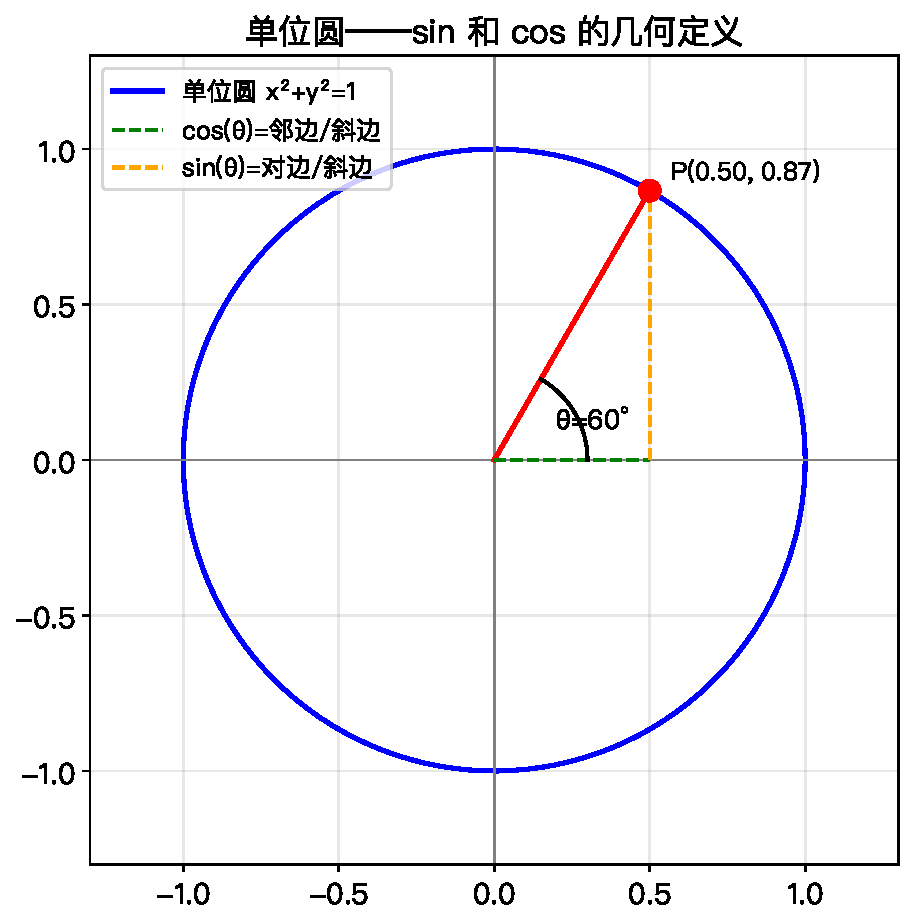
\includegraphics[width=0.5\textwidth]{figures/ch06_unit_circle.pdf}
\end{center}

以 \(\theta = 60^\circ = \dfrac{\pi}{3}\) 为例：
\[
\cos\frac{\pi}{3} = \frac{1}{2} = 0.5,\qquad
\sin\frac{\pi}{3} = \frac{\sqrt{3}}{2} \approx 0.866
\]

\textbf{验证：} \(x^2 + y^2 = (0.5)^2 + (0.866)^2 = 0.25 + 0.75 = 1\) [OK]

\textbf{关键结论：} 对任意角度 \(\theta\)：
\[
\boxed{\sin^2 \theta + \cos^2 \theta = 1}
\]
这就是\textbf{最重要的三角恒等式}。
\end{examplebox}


% ============================================================
\section{特殊角度的三角函数值}
% ============================================================

\begin{examplebox}[3——记住这几个值]
\begin{center}
\begin{tabular}{c|c|c}
\(\theta\) & \(\sin\theta\) & \(\cos\theta\) \\
\hline
\(0\) & \(0\) & \(1\) \\
\(\dfrac{\pi}{6}\) (\(30^\circ\)) & \(\dfrac{1}{2}\) & \(\dfrac{\sqrt{3}}{2}\) \\
\(\dfrac{\pi}{4}\) (\(45^\circ\)) & \(\dfrac{\sqrt{2}}{2}\) & \(\dfrac{\sqrt{2}}{2}\) \\
\(\dfrac{\pi}{3}\) (\(60^\circ\)) & \(\dfrac{\sqrt{3}}{2}\) & \(\dfrac{1}{2}\) \\
\(\dfrac{\pi}{2}\) (\(90^\circ\)) & \(1\) & \(0\) \\
\(\pi\) (\(180^\circ\)) & \(0\) & \(-1\) \\
\(\dfrac{3\pi}{2}\) (\(270^\circ\)) & \(-1\) & \(0\) \\
\(2\pi\) (\(360^\circ\)) & \(0\) & \(1\) \\
\end{tabular}
\end{center}

\textbf{记忆方法：} 从单位圆上看——
\(\sin\) 是 \(y\) 坐标（上正下负），\(\cos\) 是 \(x\) 坐标（右正左负）。
\end{examplebox}


% ============================================================
\section{正弦函数 \(y = \sin x\)}
% ============================================================

把单位圆上的 \(\sin \theta\) 值作为函数值，\(\theta\) 作为自变量，就得到正弦函数。

\begin{examplebox}[4——\(\sin x\) 的图像]
\begin{center}
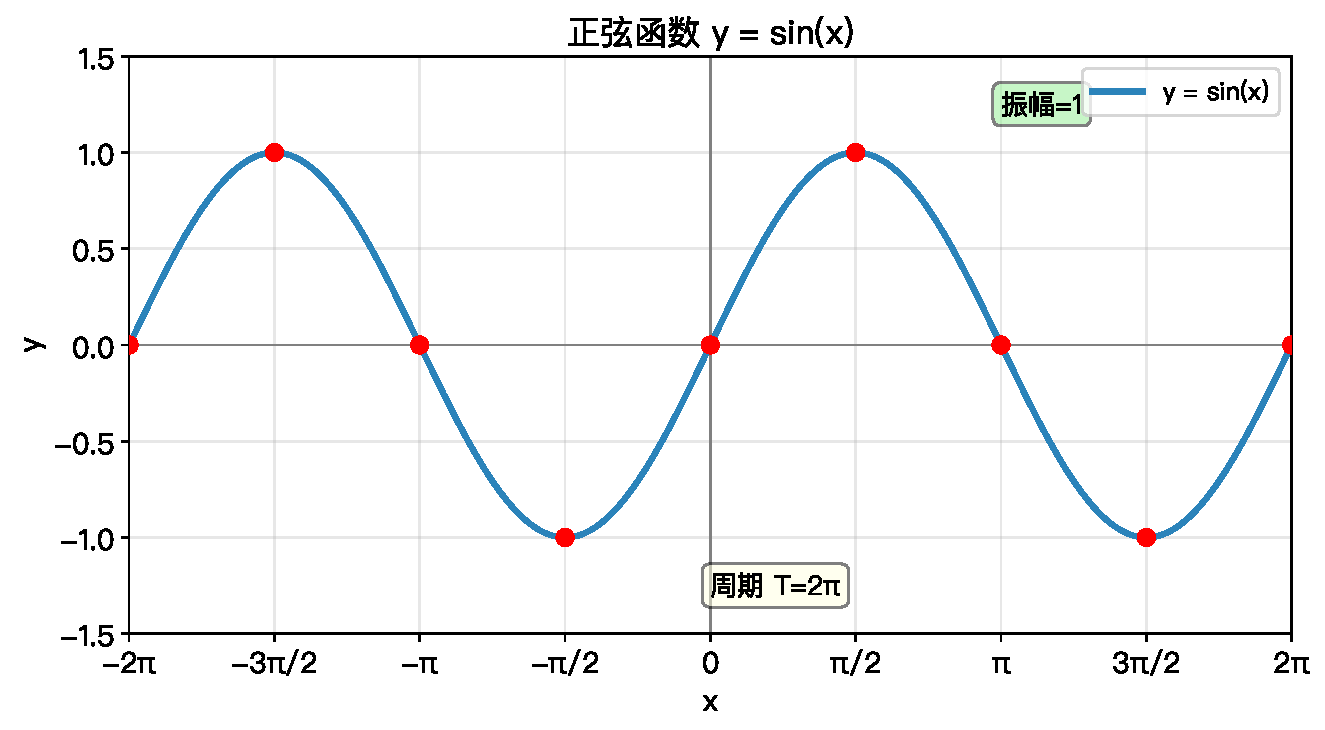
\includegraphics[width=0.85\textwidth]{figures/ch06_sine_wave.pdf}
\end{center}

\textbf{关键特征：}
\begin{enumerate}
  \item \textbf{周期性}：\(\sin(x + 2\pi) = \sin x\)——每 \(2\pi\) 重复一次
  \item \textbf{振幅}：最大值 1，最小值 \(-1\)（因为单位圆上 \(y\) 坐标在 \(-1\) 到 \(1\) 之间）
  \item \textbf{零点}：\(x = 0, \pm\pi, \pm 2\pi, \ldots\)（即 \(x = n\pi\)，\(n\) 为整数）
  \item \textbf{最大值点}：\(x = \dfrac{\pi}{2} + 2n\pi\)，\(\sin x = 1\)
  \item \textbf{最小值点}：\(x = \dfrac{3\pi}{2} + 2n\pi\)，\(\sin x = -1\)
  \item \textbf{奇函数}：\(\sin(-x) = -\sin x\)，图像关于原点对称
\end{enumerate}
\end{examplebox}

\begin{definitionbox}[正弦函数的性质]
\[
f(x) = \sin x
\]
\begin{itemize}
  \item \textbf{定义域}：\(\mathbb{R}\)（全体实数）
  \item \textbf{值域}：\([-1, 1]\)
  \item \textbf{周期}：\(T = 2\pi\)
  \item \textbf{奇偶性}：奇函数（\(\sin(-x) = -\sin x\)）
  \item \textbf{单调区间}：在 \([-\dfrac{\pi}{2}, \dfrac{\pi}{2}]\) 递增，在 \([\dfrac{\pi}{2}, \dfrac{3\pi}{2}]\) 递减
\end{itemize}
\end{definitionbox}


% ============================================================
\section{余弦函数 \(y = \cos x\)}
% ============================================================

类似地，用单位圆上的 \(x\) 坐标就得到余弦函数。

\begin{examplebox}[5——\(\cos x\) 的图像]
\begin{center}
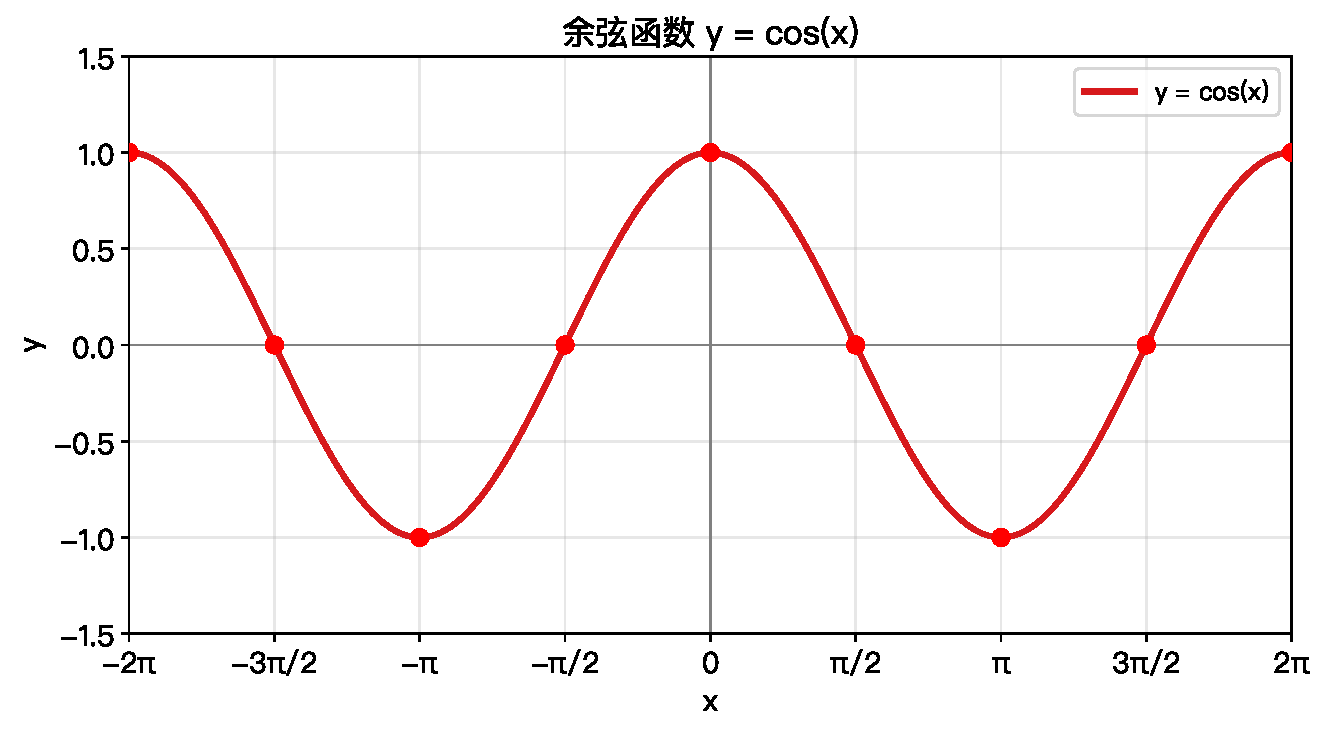
\includegraphics[width=0.85\textwidth]{figures/ch06_cosine_wave.pdf}
\end{center}

\textbf{关键特征：}
\begin{enumerate}
  \item 周期同样是 \(2\pi\)：\(\cos(x + 2\pi) = \cos x\)
  \item 值域也是 \([-1, 1]\)
  \item \textbf{偶函数}：\(\cos(-x) = \cos x\)，关于 \(y\) 轴对称
  \item \(\cos 0 = 1\)（\(\sin 0 = 0\) 的对应）
  \item 零点：\(x = \dfrac{\pi}{2} + n\pi\)
\end{enumerate}
\end{examplebox}


% ============================================================
\section{\(\sin x\) 与 \(\cos x\) 的关系}
% ============================================================

\begin{theorembox}[\(\sin\) 和 \(\cos\) 的关系]
\[
\sin\left(x + \frac{\pi}{2}\right) = \cos x, \qquad
\cos\left(x - \frac{\pi}{2}\right) = \sin x
\]

\textbf{直观理解：} \(\sin x\) 比 \(\cos x\) 领先四分之一个周期（\(\pi/2\)）。
\end{theorembox}

\begin{examplebox}[6——\(\sin\) 与 \(\cos\) 对比]
\begin{center}
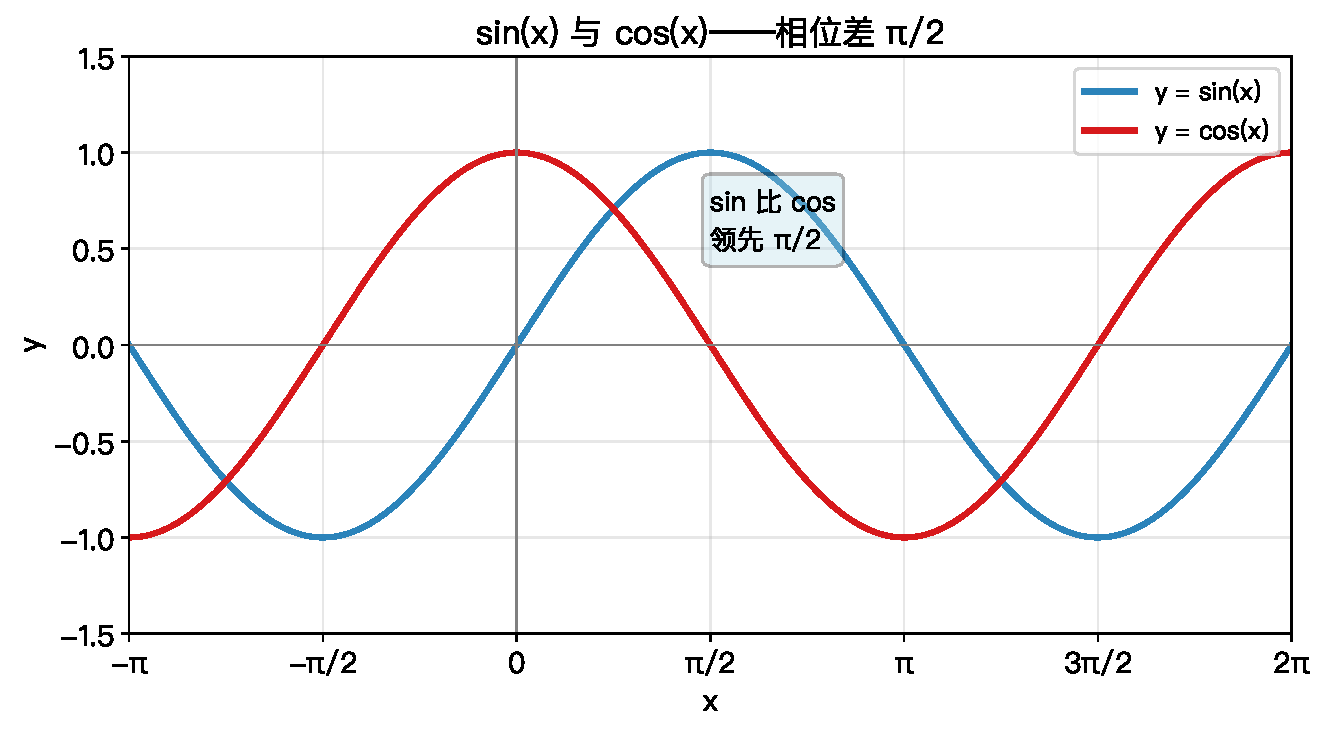
\includegraphics[width=0.85\textwidth]{figures/ch06_sine_cosine_compare.pdf}
\end{center}

\textbf{从图中可以看到：}
\begin{itemize}
  \item \(\sin x\) 在 \(x=0\) 处从 0 开始上升
  \item \(\cos x\) 在 \(x=0\) 处从 1 开始下降
  \item 把 \(\sin x\) 向左平移 \(\pi/2\) 就得到 \(\cos x\)
  \item 把 \(\cos x\) 向右平移 \(\pi/2\) 就得到 \(\sin x\)
\end{itemize}
\end{examplebox}


% ============================================================
\section{振幅与周期——控制波的形状}
% ============================================================

\begin{definitionbox}[一般形式正弦波]
\[
y = A \sin(\omega x + \varphi)
\]
其中：
\begin{itemize}
  \item \(A\) 是\textbf{振幅}——波的高度（\(|A|\)）
  \item \(\omega\) 是\textbf{角频率}——决定周期的快慢
  \item \(\varphi\) 是\textbf{初相}——决定波的起始位置
  \item \textbf{周期} \(T = \dfrac{2\pi}{\omega}\)
\end{itemize}
\end{definitionbox}

\begin{examplebox}[7——改变振幅和周期]
\begin{center}
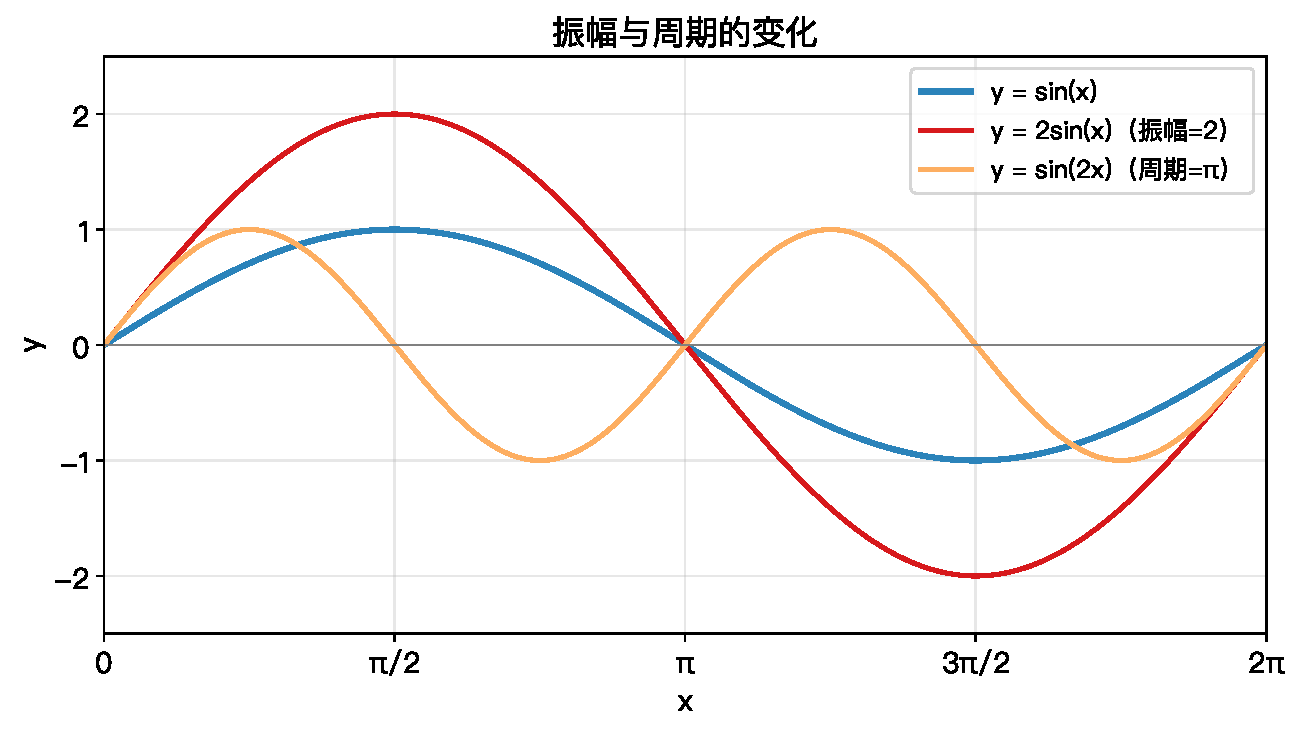
\includegraphics[width=0.85\textwidth]{figures/ch06_amplitude_period.pdf}
\end{center}

\textbf{改变振幅 \(A\)：}
\begin{itemize}
  \item \(y = \sin x\)：振幅 1，在 \(-1\) 到 \(1\) 之间
  \item \(y = 2\sin x\)：振幅 2，在 \(-2\) 到 \(2\) 之间——波更高了
\end{itemize}

\textbf{改变周期（\(\omega\)）：}
\begin{itemize}
  \item \(y = \sin x\)：周期 \(2\pi\)
  \item \(y = \sin 2x\)：周期 \(\pi\)（因为 \(T = 2\pi/2 = \pi\)）——波更密集了
\end{itemize}
\end{examplebox}


% ============================================================
\section{符号卡片}
% ============================================================

\begin{symbolcard}
\(\sin x\) & \verb|\sin x| & 读作"sin x" / "赛因 x" & 正弦函数 \\
\(\cos x\) & \verb|\cos x| & 读作"cos x" / "扣赛因 x" & 余弦函数 \\
\(\theta\) & \verb|\theta| & 读作"西塔" & 常用角度变量 \\
\(\pi\) & \verb|\pi| & 读作"派" & 圆周率，约 3.14159 \\
弧度 & —— & 读作"hú dù" & 角度的自然单位，\(180^\circ = \pi\) rad \\
周期 & —— & 读作"zhōu qī" & 函数重复一次所需的最小间隔 \\
振幅 & —— & 读作"zhèn fú" & 波峰到平衡位置的距离 \\
\end{symbolcard}


% ============================================================
\section{代码验证}
% ============================================================

\begin{lstlisting}[caption=三角函数的数值验证]
import numpy as np

# 1. 验证 sin² + cos² = 1
print("=== 验证 sin²θ + cos²θ = 1 ===")
for theta in [0, np.pi/6, np.pi/4, np.pi/3, np.pi/2, np.pi]:
    s = np.sin(theta)
    c = np.cos(theta)
    print(f"  θ={theta:5.2f}:  sin²={s**2:.6f},  cos²={c**2:.6f},  和={s**2+c**2:.6f}")

print()

# 2. 验证周期性 sin(x+2π) = sin(x)
print("=== 验证周期性 ===")
for x in [0, 0.5, 1, 2]:
    print(f"  sin({x:.1f}) = {np.sin(x):.6f},  sin({x:.1f}+2π) = {np.sin(x+2*np.pi):.6f}")

print()

# 3. 验证 sin(x+π/2) = cos(x)
print("=== 验证 sin(x+π/2) = cos(x) ===")
for x in [0, np.pi/6, np.pi/4, np.pi/3, np.pi/2]:
    lhs = np.sin(x + np.pi/2)
    rhs = np.cos(x)
    print(f"  x={x:5.2f}:  sin(x+π/2)={lhs:.6f},  cos(x)={rhs:.6f},  diff={abs(lhs-rhs):.2e}")

print()

# 4. 生成正弦波数据
print("=== 正弦波数据（前10个点）===")
x_vals = np.linspace(0, 2*np.pi, 17)  # 16等分
for x in x_vals:
    print(f"  x={x:5.2f} ({x*180/np.pi:3.0f}°):  sin={np.sin(x):7.4f},  cos={np.cos(x):7.4f}")
\end{lstlisting}

运行结果：
\begin{lstlisting}[frame=none,backgroundcolor={},numbers=none]
=== 验证 sin²θ + cos²θ = 1 ===
  θ= 0.00:  sin²=0.000000,  cos²=1.000000,  和=1.000000
  θ= 0.52:  sin²=0.250000,  cos²=0.750000,  和=1.000000
  θ= 0.79:  sin²=0.500000,  cos²=0.500000,  和=1.000000
  θ= 1.05:  sin²=0.750000,  cos²=0.250000,  和=1.000000
  θ= 1.57:  sin²=1.000000,  cos²=0.000000,  和=1.000000
  θ= 3.14:  sin²=0.000000,  cos²=1.000000,  和=1.000000
\end{lstlisting}


% ============================================================
\section{本章小结}
% ============================================================

\begin{progressbox}
\textbf{弧度制}：\(\pi\) 弧度 = \(180^\circ\)——用实数度量角度

\textbf{单位圆定义}：\(\cos\theta = x\) 坐标，\(\sin\theta = y\) 坐标

\(\sin^2 \theta + \cos^2 \theta = 1\)——最重要的三角恒等式

\textbf{正弦 }\(y = \sin x\)：周期 \(2\pi\)，值域 \([-1,1]\)，奇函数，过原点

\textbf{余弦 }\(y = \cos x\)：周期 \(2\pi\)，值域 \([-1,1]\)，偶函数，\(\cos 0 = 1\)

\textbf{相位关系}：\(\sin(x + \pi/2) = \cos x\)

\textbf{一般形式}：\(y = A \sin(\omega x + \varphi)\)，振幅 \(|A|\)，周期 \(T = 2\pi/\omega\)
\end{progressbox}

\subsection*{通往下一章}

\textbf{这一章}你学会了正弦和余弦——最基本的周期函数。

\textbf{下一章}我们继续三角函数的旅程——
正切函数、三角恒等式（和差角公式、倍角公式）、以及反三角函数。
这些是 AI 中旋转位置编码（RoPE）和傅里叶变换的基础。


% ============================================================
% 习题
% ============================================================

\section{习题}

% ===== 送分 =====

\begin{exercise}[0]
将下列度数化为弧度：
\[
(1)\; 30^\circ \qquad (2)\; 90^\circ \qquad (3)\; 180^\circ \qquad (4)\; 360^\circ
\]
\end{exercise}

\begin{exercise}[0]
求值（不用计算器）：
\[
(1)\; \sin 0 \qquad (2)\; \cos 0 \qquad (3)\; \sin \frac{\pi}{2} \qquad (4)\; \cos \pi
\]
\end{exercise}

\begin{exercise}[0]
判断正负：\(\sin 100^\circ\) 是正还是负？\(\cos 200^\circ\) 呢？
\end{exercise}

\begin{exercise}[0]
填空：\(y = \sin x\) 的周期是\_\_\_\_，值域是\_\_\_\_。
\end{exercise}

% ===== 简单 =====

\begin{exercise}[1]
求值（不用计算器，参考特殊角表格）：
\[
(1)\; \sin \frac{\pi}{6} \qquad (2)\; \cos \frac{\pi}{4} \qquad (3)\; \sin \frac{\pi}{3} \qquad (4)\; \cos \frac{\pi}{3}
\]
\end{exercise}

\begin{exercise}[1]
判断奇偶性：
\[
(1)\; y = \sin x \qquad (2)\; y = \cos x
\]
\end{exercise}

\begin{exercise}[1]
填写空白：
\[
\sin\left(x + \frac{\pi}{2}\right) = \_\_\_\_ , \qquad
\cos\left(x - \frac{\pi}{2}\right) = \_\_\_\_
\]
\end{exercise}

\begin{exercise}[1]
求 \(y = \sin x\) 在 \(x = 0, \pi/2, \pi, 3\pi/2, 2\pi\) 处的值，并画出草图。
\end{exercise}

% ===== 基础 =====

\begin{exercise}[2]
已知 \(\sin \theta = \dfrac{3}{5}\)，且 \(\theta\) 在第一象限，求 \(\cos \theta\)。
\end{exercise}

\begin{exercise}[2]
求下列函数的周期：
\[
(1)\; y = \sin 3x \qquad (2)\; y = \cos \frac{x}{2} \qquad (3)\; y = 2\sin 4x
\]
\end{exercise}

\begin{exercise}[2]
求下列函数的振幅和周期：
\[
(1)\; y = 3\sin x \qquad (2)\; y = \frac{1}{2}\cos 2x \qquad (3)\; y = -2\sin 3x
\]
\end{exercise}

\begin{exercise}[2]
判断大小（不用计算器）：
\[
(1)\; \sin 1 \text{ 和 } \cos 1 \qquad
(2)\; \sin 2 \text{ 和 } \sin 3
\]
（提示：\(\pi \approx 3.14\)，判断角度在哪个象限）
\end{exercise}

% ===== 普通 =====

\begin{exercise}[3]
化简：
\[
(1)\; \sin^2 40^\circ + \cos^2 40^\circ \qquad
(2)\; 2\sin^2 x + 2\cos^2 x \qquad
(3)\; (1 - \sin^2 x)\cos x
\]
\end{exercise}

\begin{exercise}[3]
已知 \(f(x) = 2\sin(3x)\)，求 \(f(0)\)、\(f(\pi/6)\)、\(f(\pi/2)\)。
\end{exercise}

\begin{exercise}[3]
画出 \(y = \sin x\) 和 \(y = \sin x + 1\) 在同一坐标系中的草图（一个周期即可）。
\end{exercise}

\begin{exercise}[3]
求函数 \(y = 2\cos(3x - \pi/2)\) 的：
\begin{enumerate}
  \item[(1)] 振幅
  \item[(2)] 周期
  \item[(3)] 最大值和最小值
\end{enumerate}
\end{exercise}

\begin{exercise}[3]
\(\sin 210^\circ\) 等于多少？（提示：\(210^\circ = 180^\circ + 30^\circ\)，用单位圆判断符号）
\end{exercise}

% ===== 中等 =====

\begin{exercise}[4]
证明 \(\sin(\pi - x) = \sin x\) 和 \(\cos(\pi - x) = -\cos x\)。
（提示：在单位圆上看）
\end{exercise}

\begin{exercise}[4]
解方程 \(\sin x = \dfrac{1}{2}\)，\(x \in [0, 2\pi)\)。
\end{exercise}

\begin{exercise}[4]
已知函数 \(y = 3\sin(2x - \pi/3)\)。
\begin{enumerate}
  \item[(1)] 求振幅、周期、初相
  \item[(2)] 求在 \(x=0\) 处的函数值
  \item[(3)] 这个函数是由 \(y = \sin x\) 经过怎样的变换得到的？
\end{enumerate}
\end{exercise}

\begin{exercise}[4]
弹簧振子的位移 \(d(t) = 5\cos(2\pi t)\)，其中 \(t\) 是时间（秒）。
\begin{enumerate}
  \item[(1)] 求振幅和周期
  \item[(2)] \(t=0\) 时位移是多少？
  \item[(3)] 什么时刻位移为 0？
\end{enumerate}
\end{exercise}

\begin{exercise}[4]
验证 \(\sin(x + \pi) = -\sin x\) 和 \(\cos(x + \pi) = -\cos x\)，
并用这个性质解释为什么 \(\sin x\) 和 \(\cos x\) 的周期是 \(2\pi\)。
\end{exercise}

% ===== 进阶 =====

\begin{exercise}[5]
求函数 \(y = \sin x + \sqrt{3}\cos x\) 的最大值。
（提示：利用公式 \(a\sin x + b\cos x = \sqrt{a^2 + b^2}\sin(x + \varphi)\)）
\end{exercise}

\begin{exercise}[5]
已知 \(\sin^2 \theta + \cos \theta = 1\)，且 \(0 \le \theta \le 2\pi\)，求 \(\theta\)。
\end{exercise}

\begin{exercise}[5]
一个交流电压 \(V(t) = 220\sin(100\pi t)\)（\(t\) 为秒）。
\begin{enumerate}
  \item[(1)] 求电压的周期和频率（频率 = 1/周期）
  \item[(2)] 求电压的最大值
  \item[(3)] 在 \(t = 0.005\) 秒时电压是多少？
\end{enumerate}
\end{exercise}

\begin{exercise}[5]
已知 \(f(x) = \sin x + \cos x\)。
\begin{enumerate}
  \item[(1)] 求 \(f(x)\) 的最大值和最小值
  \item[(2)] 求 \(f(x)\) 的周期
\end{enumerate}
\end{exercise}

% ===== 拔高 =====

\begin{exercise}[6]
已知 \(\sin \theta + \cos \theta = \dfrac{1}{2}\)，求：
\[
(1)\; \sin \theta \cos \theta \qquad (2)\; \sin^3 \theta + \cos^3 \theta
\]
（提示：利用 \((\sin\theta + \cos\theta)^2 = 1 + 2\sin\theta\cos\theta\)）
\end{exercise}

\begin{exercise}[6]
函数 \(y = \sin x\) 的图像经过以下变换，写出新函数的表达式：
\[
y = \sin x \xrightarrow{\text{纵坐标伸长为2倍}} \xrightarrow{\text{横坐标压缩为1/3}} \xrightarrow{\text{向右平移 }\pi/4}
\]
\end{exercise}

\begin{exercise}[6]
求证 \(\dfrac{1 - 2\sin^2 x}{\cos x + \sin x} = \cos x - \sin x\)。
\end{exercise}

% ===== 极难 =====

\begin{exercise}[7]
已知 \(f(x) = |\sin x| + |\cos x|\)。
\begin{enumerate}
  \item[(1)] 求 \(f(x)\) 的周期（提示：画图或用数值试探）
  \item[(2)] 求 \(f(x)\) 的值域
  \item[(3)] 验证：\([f(x)]^2 = 1 + |\sin 2x|\)
\end{enumerate}

\textbf{说明：} 这道题结合了绝对值、三角函数和周期，需要画图辅助思考。
绝对值函数的周期往往比原函数更短——这是一个重要的观察。
\end{exercise}

% ============================================================
% 第7章：三角函数（下）——正切、恒等式、反三角
% ============================================================

\chapter{三角函数（下）——正切、恒等式、反三角}

\begin{applicationbox}
\textbf{学完本章你能做什么？}
\begin{enumerate}
  \item 学会 \(\tan x\) 的图像和性质，能对比 \(\sin, \cos, \tan\) 的异同
  \item 掌握三角恒等式——和差角公式、倍角公式——它们是 AI 中 RoPE 位置编码的基础
  \item 会使用反三角函数 \(\arcsin, \arccos, \arctan\)——从三角函数值反推角度
\end{enumerate}
\end{applicationbox}


% ============================================================
\section{从第6章来——还需要更多}
% ============================================================

第6章我们学了 \(\sin x\) 和 \(\cos x\)——最基本的两个三角函数。

但还有 \(\tan x\)、更多的恒等式、以及逆运算（反三角函数）需要掌握。\\
这些知识在 Transformer 的位置编码（RoPE）、傅里叶变换、信号处理中都会用到。


% ============================================================
\section{正切函数 \(\tan x\)}
% ============================================================

\begin{definitionbox}[正切函数]
\[
\tan x = \frac{\sin x}{\cos x}, \quad \cos x \neq 0
\]

读作"tan x"（摊进塔 x），英文 tangent。
\end{definitionbox}

\begin{examplebox}[1——\(\tan x\) 的图像]
\begin{center}
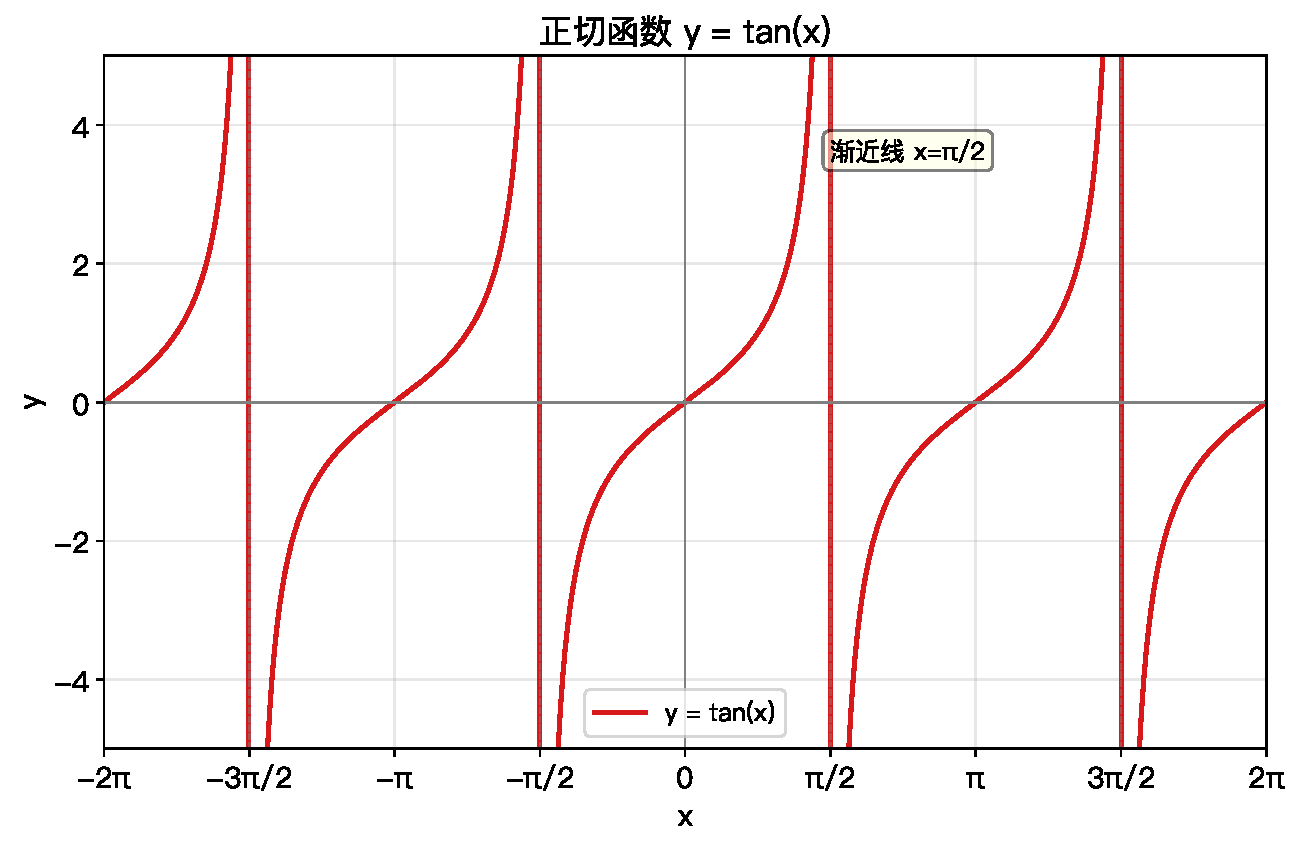
\includegraphics[width=0.85\textwidth]{figures/ch07_tangent.pdf}
\end{center}

\textbf{关键特征：}
\begin{enumerate}
  \item \textbf{周期}：\(\pi\)（不是 \(2\pi\)！）——因为 \(\tan(x+\pi) = \tan x\)
  \item \textbf{定义域}：\(x \neq \dfrac{\pi}{2} + n\pi\)（\(\cos x = 0\) 的点）
  \item \textbf{值域}：\(\mathbb{R}\)（可以取任意实数）
  \item \textbf{渐近线}：在 \(x = \dfrac{\pi}{2} + n\pi\) 处有垂直渐近线
  \item \textbf{奇函数}：\(\tan(-x) = -\tan x\)
  \item \textbf{特殊值}：\(\tan 0 = 0\)，\(\tan \dfrac{\pi}{4} = 1\)，\(\tan \pi = 0\)
\end{enumerate}
\end{examplebox}


% ============================================================
\section{\(\sin, \cos, \tan\) 对比}
% ============================================================

\begin{examplebox}[2——三大三角函数同框]
\begin{center}
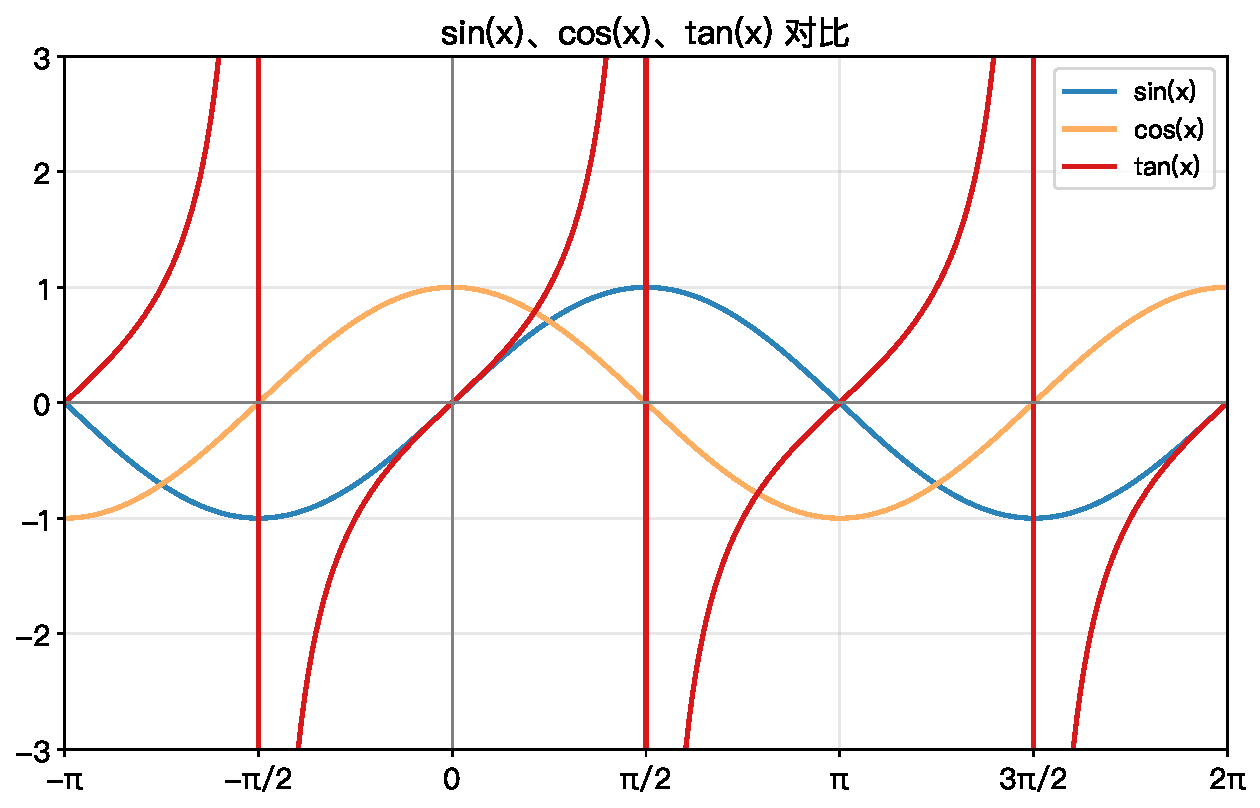
\includegraphics[width=0.85\textwidth]{figures/ch07_sin_cos_tan.pdf}
\end{center}

\begin{center}
\begin{tabular}{c|c|c|c}
 & \(\sin x\) & \(\cos x\) & \(\tan x\) \\
\hline
定义域 & \(\mathbb{R}\) & \(\mathbb{R}\) & \(x \neq \pi/2 + n\pi\) \\
值域 & \([-1, 1]\) & \([-1, 1]\) & \(\mathbb{R}\) \\
周期 & \(2\pi\) & \(2\pi\) & \(\pi\) \\
奇偶性 & 奇 & 偶 & 奇 \\
零点 & \(n\pi\) & \(\pi/2 + n\pi\) & \(n\pi\) \\
\end{tabular}
\end{center}
\end{examplebox}


% ============================================================
\section{三角恒等式——最重要的公式}
% ============================================================

\subsection{和差角公式}

\begin{theorembox}[和差角公式]
\begin{align*}
\sin(a \pm b) &= \sin a \cos b \pm \cos a \sin b \\
\cos(a \pm b) &= \cos a \cos b \mp \sin a \sin b \\
\tan(a \pm b) &= \frac{\tan a \pm \tan b}{1 \mp \tan a \tan b}
\end{align*}
\end{theorembox}

\begin{examplebox}[3——用和差角公式求 \(\sin 75^\circ\)]
\[
\sin 75^\circ = \sin(45^\circ + 30^\circ) = \sin 45^\circ \cos 30^\circ + \cos 45^\circ \sin 30^\circ
\]
\[
= \frac{\sqrt{2}}{2} \cdot \frac{\sqrt{3}}{2} + \frac{\sqrt{2}}{2} \cdot \frac{1}{2}
= \frac{\sqrt{6} + \sqrt{2}}{4} \approx 0.9659
\]

\textbf{验证：} 计算器 \(\sin 75^\circ \approx 0.9659\) [OK]
\end{examplebox}

\subsection{倍角公式}

\begin{theorembox}[倍角公式]
由和差角公式令 \(a = b = x\) 得到：
\begin{align*}
\sin 2x &= 2\sin x \cos x \\
\cos 2x &= \cos^2 x - \sin^2 x = 1 - 2\sin^2 x = 2\cos^2 x - 1
\end{align*}
\end{theorembox}

\begin{examplebox}[4——倍角公式的应用]
已知 \(\sin x = \dfrac{3}{5}\)（\(x\) 在第一象限），求 \(\sin 2x\)。

解：
\[
\cos x = \sqrt{1 - \sin^2 x} = \sqrt{1 - \frac{9}{25}} = \sqrt{\frac{16}{25}} = \frac{4}{5}
\]
\[
\sin 2x = 2\sin x \cos x = 2 \cdot \frac{3}{5} \cdot \frac{4}{5} = \frac{24}{25}
\]
\end{examplebox}

\subsection{半角公式}

\begin{theorembox}[半角公式]
由倍角公式变形得到：
\[
\sin^2 \frac{x}{2} = \frac{1 - \cos x}{2}, \qquad
\cos^2 \frac{x}{2} = \frac{1 + \cos x}{2}
\]
\end{theorembox}


% ============================================================
\section{反三角函数——从值反推角度}
% ============================================================

如果 \(\sin \theta = 0.5\)，那 \(\theta\) 是多少？\\
我们知道 \(\theta = \pi/6\) 是一个答案，但还有 \(\theta = 5\pi/6\)……有无穷多个。

我们需要\textbf{限制值域}，使反函数成为单值函数。

\begin{definitionbox}[反三角函数]
\begin{center}
\begin{tabular}{c|c|c}
\textbf{函数} & \textbf{定义域} & \textbf{值域} \\
\hline
\(y = \arcsin x\)（或 \(\sin^{-1} x\)） & \([-1, 1]\) & \([-\pi/2,\; \pi/2]\) \\
\(y = \arccos x\)（或 \(\cos^{-1} x\)） & \([-1, 1]\) & \([0,\; \pi]\) \\
\(y = \arctan x\)（或 \(\tan^{-1} x\)） & \(\mathbb{R}\) & \((-\pi/2,\; \pi/2)\) \\
\end{tabular}
\end{center}

\textbf{读法：} \(\arcsin x\) 读作"阿克赛因 x"，\(\arccos x\) 读作"阿克扣赛因 x"。
\end{definitionbox}

\begin{examplebox}[5——\(\arcsin x\) 和 \(\arccos x\)]
\begin{center}
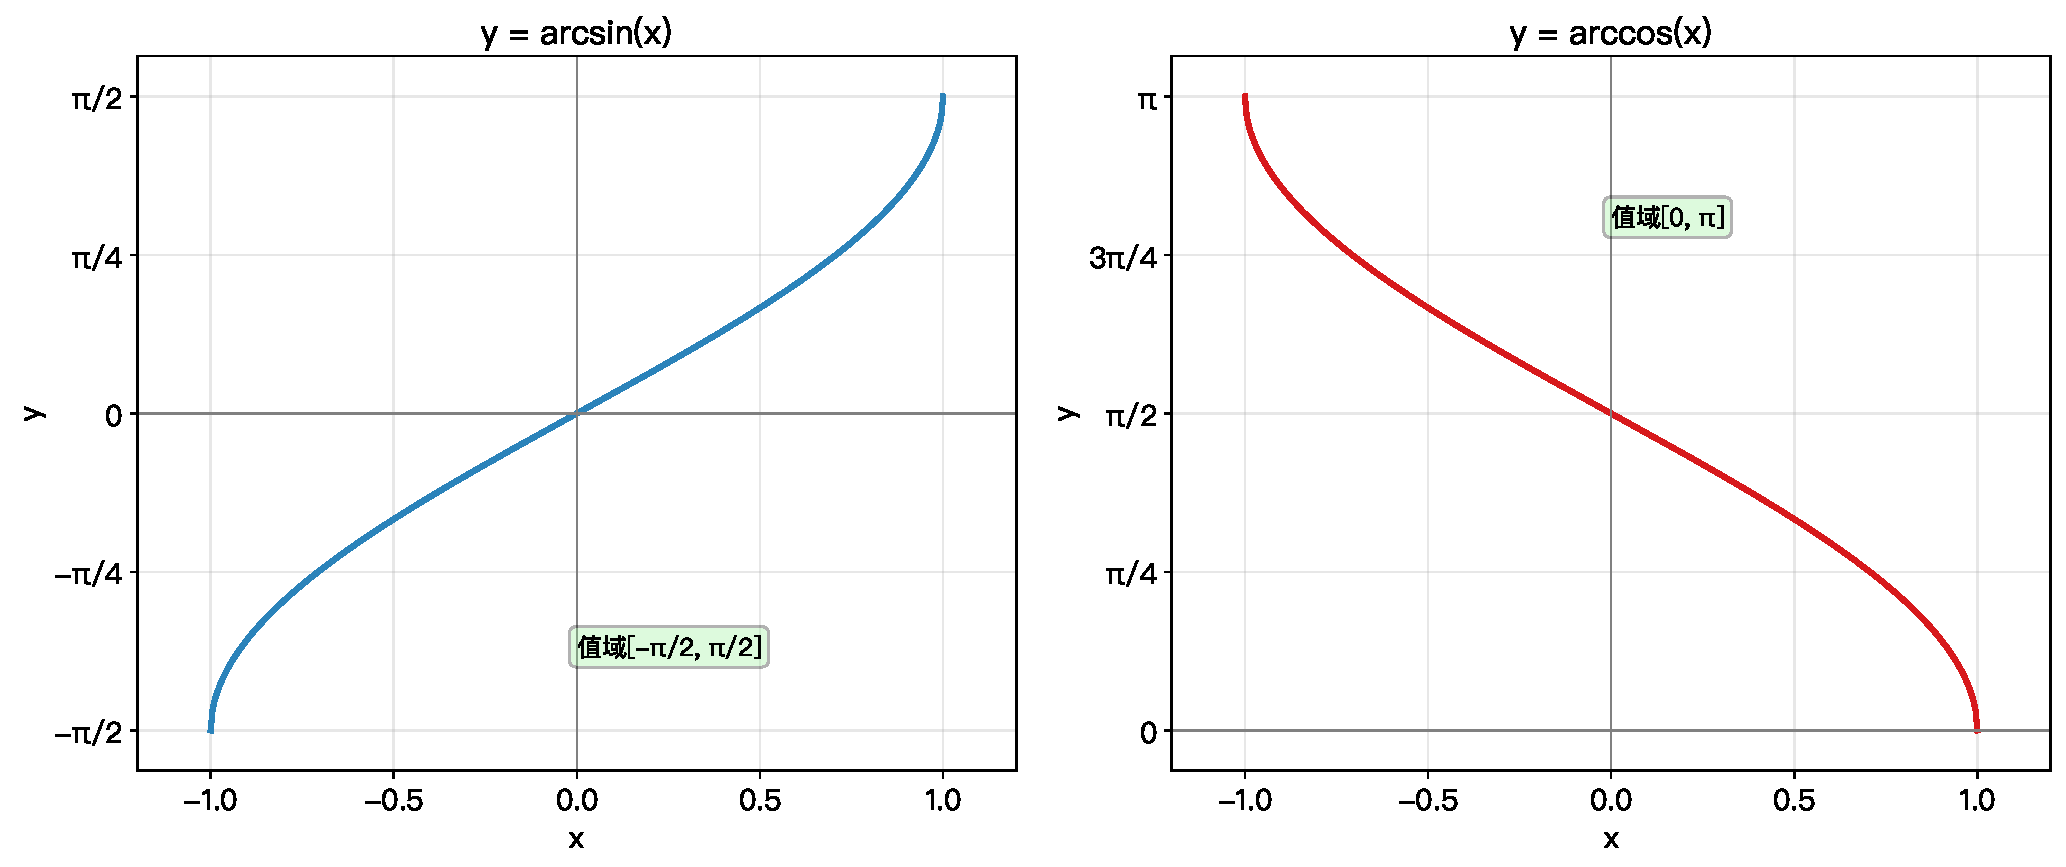
\includegraphics[width=0.85\textwidth]{figures/ch07_arcsin_arccos.pdf}
\end{center}

\textbf{关键理解：}
\begin{itemize}
  \item \(\arcsin(0.5) = \dfrac{\pi}{6}\)（值域在 \([-\pi/2, \pi/2]\)，所以取 \(\pi/6\) 而不是 \(5\pi/6\)）
  \item \(\arccos(0.5) = \dfrac{\pi}{3}\)（值域在 \([0, \pi]\)）
  \item \(\arcsin(\sin x) = x\) 只在 \(x \in [-\pi/2, \pi/2]\) 时成立
\end{itemize}
\end{examplebox}

\begin{examplebox}[6——\(\arctan x\)]
\begin{center}
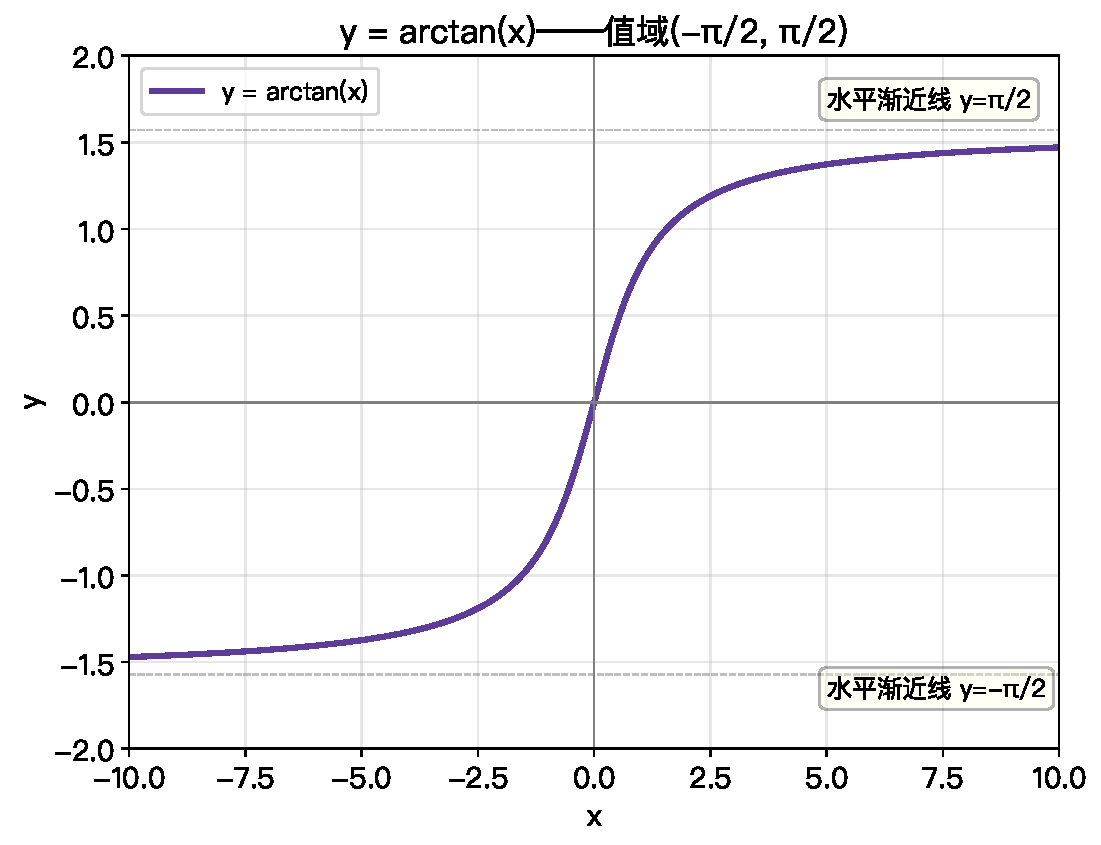
\includegraphics[width=0.55\textwidth]{figures/ch07_arctan.pdf}
\end{center}

\(\arctan x\) 的特点：
\begin{itemize}
  \item 定义域为全体实数，值域为 \((-\pi/2, \pi/2)\)
  \item 有两条水平渐近线：\(y = \pi/2\) 和 \(y = -\pi/2\)
  \item \(\arctan 1 = \pi/4\)，\(\arctan 0 = 0\)
  \item AI 中常用于将任意实数映射到有限范围（如 Sigmoid 的替代）
\end{itemize}
\end{examplebox}


% ============================================================
\section{三角函数在 AI 中的应用——RoPE 直觉}
% ============================================================

\begin{examplebox}[7——旋转位置编码 (RoPE)]
Transformer 模型需要知道词的位置信息。RoPE（旋转位置编码）用三角函数来编码位置：

\[
\text{位置 } m \text{ 的编码} = \begin{pmatrix}
\cos m\theta & -\sin m\theta \\
\sin m\theta & \cos m\theta
\end{pmatrix}
\begin{pmatrix}
x \\
y
\end{pmatrix}
\]

这其实就是\textbf{旋转}一个二维向量 \((x, y)\)——旋转的角度和位置 \(m\) 成正比。

\textbf{为什么用三角函数？}
\begin{enumerate}
  \item 旋转不改变向量长度（\(\sin^2 + \cos^2 = 1\)）
  \item 相对位置的关系可以用和差角公式简洁表达
  \item 位置越远，旋转角度越大
\end{enumerate}

这就是为什么 Transformer 能"知道"词与词的相对距离——三角函数在背后起了关键作用。
\end{examplebox}


% ============================================================
\section{符号卡片}
% ============================================================

\begin{symbolcard}
\(\tan x\) & \verb|\tan x| & 读作"tan x" & \(\sin x / \cos x\) \\
\(\arcsin x\) & \verb|\arcsin x| & 读作"阿克赛因" & \(\sin\) 的反函数，值域 \([-\pi/2,\pi/2]\) \\
\(\arccos x\) & \verb|\arccos x| & 读作"阿克扣赛因" & \(\cos\) 的反函数，值域 \([0,\pi]\) \\
\(\arctan x\) & \verb|\arctan x| & 读作"阿克坦进特" & \(\tan\) 的反函数，值域 \((-\pi/2,\pi/2)\) \\
\end{symbolcard}


% ============================================================
\section{代码验证}
% ============================================================

\begin{lstlisting}[caption=三角恒等式的数值验证]
import numpy as np

# 1. 验证和差角公式
print("=== 和差角公式 ===")
a, b = np.pi/3, np.pi/6
lhs = np.sin(a + b)
rhs = np.sin(a)*np.cos(b) + np.cos(a)*np.sin(b)
print(f"  sin(π/3+π/6) = {lhs:.6f},  公式 = {rhs:.6f}, diff = {abs(lhs-rhs):.2e}")

lhs = np.cos(a - b)
rhs = np.cos(a)*np.cos(b) + np.sin(a)*np.sin(b)
print(f"  cos(π/3-π/6) = {lhs:.6f},  公式 = {rhs:.6f}, diff = {abs(lhs-rhs):.2e}")

print()

# 2. 验证倍角公式
print("=== 倍角公式 ===")
for x in [0.2, 0.5, 1.0, 1.5]:
    lhs = np.sin(2*x)
    rhs = 2*np.sin(x)*np.cos(x)
    print(f"  x={x:.2f}:  sin(2x)={lhs:.6f}, 2sin(x)cos(x)={rhs:.6f}")

print()

# 3. 验证反三角函数
print("=== 反三角函数 ===")
for val in [-1, -0.5, 0, 0.5, 1]:
    print(f"  arcsin({val:4.1f}) = {np.arcsin(val):.4f} rad = {np.degrees(np.arcsin(val)):.1f}°")
    print(f"  arccos({val:4.1f}) = {np.arccos(val):.4f} rad = {np.degrees(np.arccos(val)):.1f}°")

print()

# 4. 验证 tan = sin/cos
print("=== 验证 tan = sin/cos ===")
for x in [0.2, 0.5, 0.8, 1.0]:
    if abs(np.cos(x)) > 1e-10:
        print(f"  tan({x:.2f}) = {np.tan(x):.6f}, sin/cos = {np.sin(x)/np.cos(x):.6f}")
\end{lstlisting}

运行结果：
\begin{lstlisting}[frame=none,backgroundcolor={},numbers=none]
=== 和差角公式 ===
  sin(π/3+π/6) = 1.000000,  公式 = 1.000000, diff = 0.00e+00
  cos(π/3-π/6) = 0.866025,  公式 = 0.866025, diff = 0.00e+00

=== 倍角公式 ===
  x=0.20:  sin(2x)=0.389418, 2sin(x)cos(x)=0.389418
  x=0.50:  sin(2x)=0.841471, 2sin(x)cos(x)=0.841471
  x=1.00:  sin(2x)=0.909297, 2sin(x)cos(x)=0.909297
\end{lstlisting}


% ============================================================
\section{本章小结}
% ============================================================

\begin{progressbox}
\textbf{正切} \(\tan x = \dfrac{\sin x}{\cos x}\)，周期 \(\pi\)，有垂直渐近线

\textbf{和差角公式}：\(\sin(a\pm b)\)、\(\cos(a\pm b)\)、\(\tan(a\pm b)\)

\textbf{倍角公式}：\(\sin 2x = 2\sin x \cos x\)，\(\cos 2x = \cos^2 x - \sin^2 x\)

\textbf{反三角函数}：\(\arcsin\)（值域 \([-\pi/2,\pi/2]\)）、\(\arccos\)（\([0,\pi]\)）、\(\arctan\)（\((-\pi/2,\pi/2)\)）

\textbf{AI 应用}：RoPE（旋转位置编码）用三角恒等式编码位置信息
\end{progressbox}

\subsection*{通往下一章}

\textbf{这一章}完成了三角函数的全部核心知识。

\textbf{下一章——第0编的最后一章}，我们将回归函数本身，系统地学习\textbf{函数的四大性质}：
单调性、奇偶性、周期性、有界性，以及复合函数与反函数的完整理论。
这标志着"函数基础重建"阶段的收官。


% ============================================================
% 习题
% ============================================================
\section{习题}

% ===== 送分 =====

\begin{exercise}[0]
求值（不用计算器）：
\[
(1)\; \tan 0 \qquad (2)\; \tan \frac{\pi}{4} \qquad (3)\; \tan \pi \qquad (4)\; \tan \frac{3\pi}{4}
\]
\end{exercise}

\begin{exercise}[0]
求值（不用计算器）：
\[
(1)\; \arcsin 0 \qquad (2)\; \arcsin 1 \qquad (3)\; \arccos 1 \qquad (4)\; \arctan 1
\]
\end{exercise}

\begin{exercise}[0]
判断正误：\(\tan x\) 的周期是 \(2\pi\)（是/否）
\end{exercise}

\begin{exercise}[0]
填空：\(\tan x = \dfrac{\sin x}{\_\_\_\_}\)，定义域为 \(x \neq \_\_\_\_ + n\pi\)。
\end{exercise}

% ===== 简单 =====

\begin{exercise}[1]
已知 \(\sin x = \dfrac{1}{2}\)，\(\cos x = \dfrac{\sqrt{3}}{2}\)，求 \(\tan x\)。
\end{exercise}

\begin{exercise}[1]
判断奇偶性：
\[
(1)\; y = \tan x \qquad (2)\; y = \arcsin x \qquad (3)\; y = \arccos x
\]
\end{exercise}

\begin{exercise}[1]
求值：
\[
(1)\; \sin\frac{\pi}{3}\cos\frac{\pi}{6} + \cos\frac{\pi}{3}\sin\frac{\pi}{6} \qquad
(2)\; \cos\frac{\pi}{4}\cos\frac{\pi}{4} - \sin\frac{\pi}{4}\sin\frac{\pi}{4}
\]
\end{exercise}

\begin{exercise}[1]
求 \(\arctan(-\sqrt{3})\) 的值（弧度表示）。
\end{exercise}

% ===== 基础 =====

\begin{exercise}[2]
用倍角公式化简：
\[
(1)\; 2\sin 15^\circ \cos 15^\circ \qquad
(2)\; \cos^2 22.5^\circ - \sin^2 22.5^\circ
\]
\end{exercise}

\begin{exercise}[2]
已知 \(\cos x = \dfrac{3}{5}\)，\(x\) 在第四象限，求 \(\tan x\)。
\end{exercise}

\begin{exercise}[2]
求下列函数的值域：
\[
(1)\; y = \arcsin x \qquad (2)\; y = \arccos x \qquad (3)\; y = \arctan x
\]
\end{exercise}

\begin{exercise}[2]
求证 \(\tan x \cdot \cot x = 1\)（\(\cot x = \dfrac{\cos x}{\sin x}\) 是余切）。
\end{exercise}

% ===== 普通 =====

\begin{exercise}[3]
已知 \(\sin \alpha = \dfrac{3}{5}\)，\(\alpha\) 在第一象限，\(\cos \beta = -\dfrac{5}{13}\)，\(\beta\) 在第二象限。
求 \(\sin(\alpha + \beta)\) 和 \(\cos(\alpha - \beta)\)。
\end{exercise}

\begin{exercise}[3]
用和差角公式求 \(\cos 15^\circ\) 的值（保留根号形式）。
\end{exercise}

\begin{exercise}[3]
求证：
\[
\sin(x + \pi) = -\sin x,\quad \cos(x + \pi) = -\cos x,\quad \tan(x + \pi) = \tan x
\]
\end{exercise}

\begin{exercise}[3]
已知 \(\sin 2x = \dfrac{4}{5}\)，\(x\) 在第一象限，求 \(\sin x\) 和 \(\cos x\)。
\end{exercise}

\begin{exercise}[3]
求值：
\[
\arcsin\left(-\frac{1}{2}\right) + \arccos\left(\frac{1}{2}\right)
\]
\end{exercise}

% ===== 中等 =====

\begin{exercise}[4]
已知 \(\tan x = 2\)，求：
\[
(1)\; \frac{\sin x + \cos x}{\sin x - \cos x} \qquad
(2)\; \sin^2 x + \sin x \cos x
\]
\end{exercise}

\begin{exercise}[4]
求证 \(\cos^4 x - \sin^4 x = \cos 2x\)。
\end{exercise}

\begin{exercise}[4]
解方程 \(\tan x = 1\)，\(x \in [0, 2\pi)\)。
\end{exercise}

\begin{exercise}[4]
化简：
\[
\sin(30^\circ + x) - \sin(30^\circ - x)
\]
\end{exercise}

\begin{exercise}[4]
在 \(\triangle ABC\) 中，已知 \(\sin A = \dfrac{3}{5}\)，\(\cos B = \dfrac{5}{13}\)，求 \(\cos C\)。
（提示：\(A + B + C = \pi\)，\(\cos C = -\cos(A+B)\)）
\end{exercise}

% ===== 进阶 =====

\begin{exercise}[5]
求证：
\[
\frac{\sin 2x}{1 + \cos 2x} = \tan x
\]
\end{exercise}

\begin{exercise}[5]
已知 \(\sin x + \cos x = \dfrac{1}{\sqrt{2}}\)，求 \(\sin 2x\)。
\end{exercise}

\begin{exercise}[5]
求函数 \(y = \tan\left(2x - \dfrac{\pi}{3}\right)\) 的：
\begin{enumerate}
  \item[(1)] 定义域
  \item[(2)] 周期
  \item[(3)] 渐近线方程
\end{enumerate}
\end{exercise}

\begin{exercise}[5]
已知 \(\tan \alpha = 2\)，\(\tan \beta = 3\)，求 \(\tan(\alpha + \beta)\) 和 \(\alpha + \beta\)（\(\alpha, \beta \in (0, \pi/2)\)）。
\end{exercise}

% ===== 拔高 =====

\begin{exercise}[6]
已知函数 \(f(x) = \arctan x + \arctan \dfrac{1 - x}{1 + x}\)（\(x \neq -1\)）。
\begin{enumerate}
  \item[(1)] 计算 \(f(0)\)、\(f(1)\)、\(f(\sqrt{3})\)
  \item[(2)] 猜想 \(f(x)\) 的值（提示：利用 \(\tan\) 的和角公式）
\end{enumerate}
\end{exercise}

\begin{exercise}[6]
求证：
\[
\arcsin x + \arccos x = \frac{\pi}{2}, \quad x \in [-1, 1]
\]
\end{exercise}

\begin{exercise}[6]
已知 \(\sin \theta + \sin 2\theta + \sin 3\theta = 0\)，求 \(\theta \in [0, 2\pi)\)。
（提示：利用和差化积公式 \(\sin A + \sin B = 2\sin\frac{A+B}{2}\cos\frac{A-B}{2}\)）
\end{exercise}

% ===== 极难 =====

\begin{exercise}[7]
已知函数 \(f(x) = \sin(\arctan x)\)。
\begin{enumerate}
  \item[(1)] 化简 \(f(x)\)（提示：构造直角三角形，对边 \(x\)，邻边 \(1\)）
  \item[(2)] 求 \(f(x)\) 的值域
  \item[(3)] 求 \(f(f(x))\) 的表达式
\end{enumerate}

\textbf{说明：} 这道题把三角函数和反三角函数结合在一起，
需要利用几何直观（直角三角形）来化简代数表达式。
这是数学分析中常见的技巧——"几何图像引导代数推导"。
\end{exercise}

% ============================================================
% 第8章：函数的四大性质 + 复合与反函数
% ============================================================

\chapter{函数的四大性质——单调·奇偶·周期·有界}

\begin{applicationbox}
\textbf{学完本章你能做什么？}
\begin{enumerate}
  \item 系统掌握函数的四大性质——\textbf{单调性、奇偶性、周期性、有界性}
  \item 理解\textbf{复合函数}的"链式"结构和\textbf{反函数}的对称性
  \item 标志第0编"函数基础重建"的收官——你已经为数学分析做好了全部准备！
\end{enumerate}
\end{applicationbox}


% ============================================================
\section{从第7章来——总结与升华}
% ============================================================

前7章我们一一认识了各种函数：幂函数、指数函数、对数函数、三角函数。

这一章我们回到\textbf{函数本身}，系统地学习函数的四大基本性质。
这些性质不是某个函数特有的——\textbf{每个函数都可以从这四个维度来分析}。

\begin{center}
\fcolorbox{teal!50}{teal!5}{\parbox{0.85\textwidth}{
\textbf{函数的四大性质：}
\[
\text{单调性} \;\longrightarrow\; \text{增长还是衰减？}
\]
\[
\text{奇偶性} \;\longrightarrow\; \text{对称还是不对称？}
\]
\[
\text{周期性} \;\longrightarrow\; \text{重复还是不重复？}
\]
\[
\text{有界性} \;\longrightarrow\; \text{在范围内还是无限延伸？}
\]
}}
\end{center}


% ============================================================
\section{单调性——递增还是递减？}
% ============================================================

\begin{definitionbox}[单调性]
设函数 \(f(x)\) 在区间 \(I\) 上有定义。
\begin{itemize}
  \item 如果对任意 \(x_1 < x_2\) 都有 \(f(x_1) < f(x_2)\)，则称 \(f\) 在 \(I\) 上\textbf{单调递增}
  \item 如果对任意 \(x_1 < x_2\) 都有 \(f(x_1) > f(x_2)\)，则称 \(f\) 在 \(I\) 上\textbf{单调递减}
\end{itemize}
\end{definitionbox}

\begin{examplebox}[1——单调性直观对比]
\begin{center}
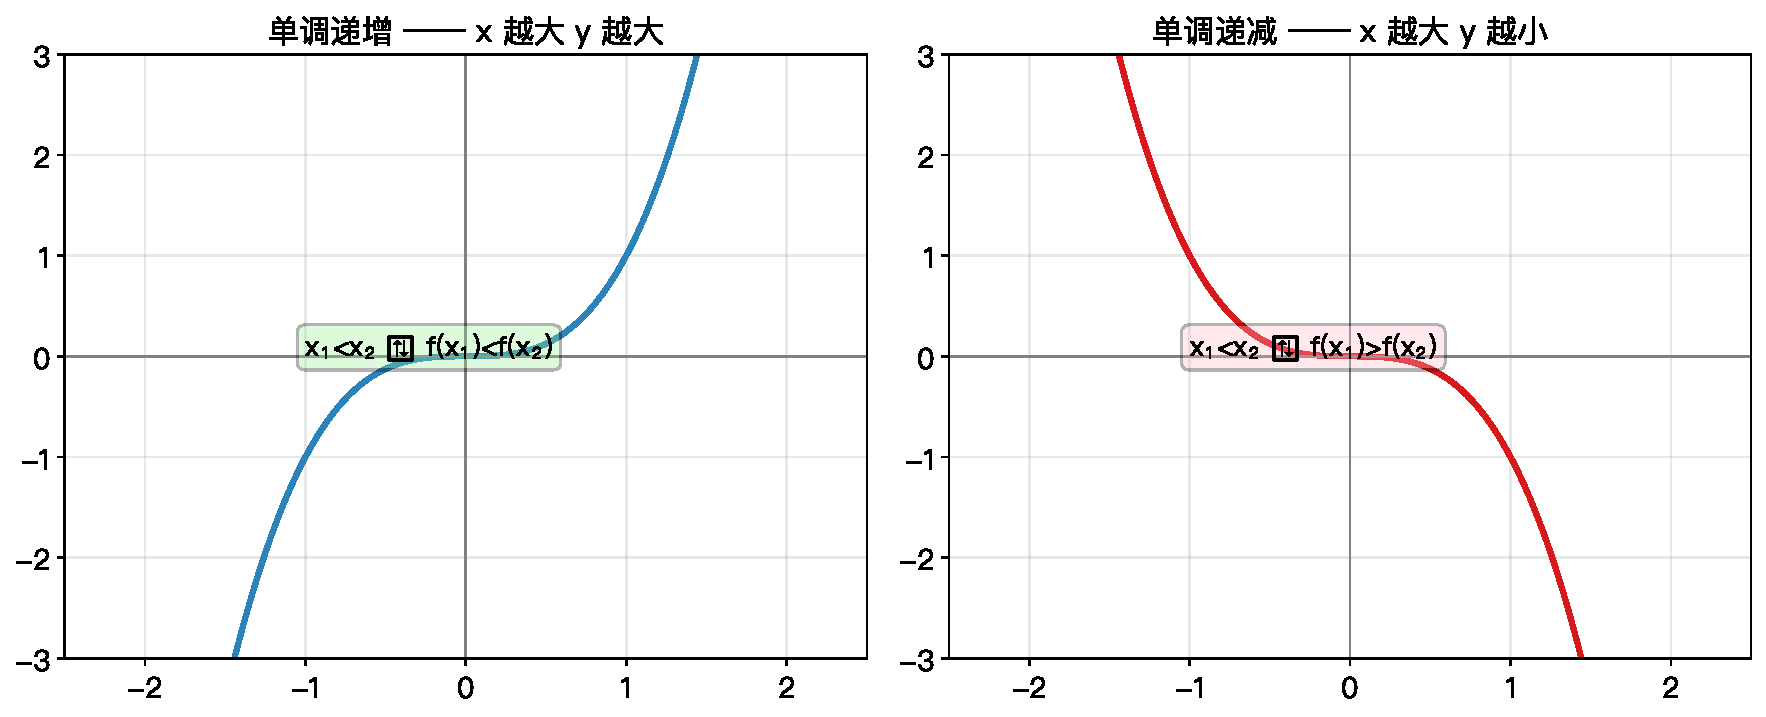
\includegraphics[width=0.85\textwidth]{figures/ch08_monotonic.pdf}
\end{center}

\textbf{左图}（\(y = x^3\)）：从左到右一路向上——单调递增。\\
\textbf{右图}（\(y = -x^3\)）：从左到右一路向下——单调递减。
\end{examplebox}

\begin{examplebox}[2——判断单调性]
判断 \(f(x) = 2^x\) 的单调性。

解：取任意 \(x_1 < x_2\)，则 \(2^{x_1} < 2^{x_2}\)（因为底数 \(2>1\)）。
所以 \(f(x_1) < f(x_2)\) \(\rightarrow\) \textbf{单调递增}。

判断 \(f(x) = (1/2)^x\) 的单调性：
取任意 \(x_1 < x_2\)，则 \((1/2)^{x_1} > (1/2)^{x_2}\)（因为底数 \(1/2 < 1\)）。
所以 \(f(x_1) > f(x_2)\) \(\rightarrow\) \textbf{单调递减}。
\end{examplebox}


% ============================================================
\section{奇偶性——对称还是不对称？}
% ============================================================

\begin{definitionbox}[奇偶性]
设函数 \(f(x)\) 的定义域关于原点对称。
\begin{itemize}
  \item 如果 \(f(-x) = f(x)\) 对所有 \(x\) 成立，则称 \(f\) 是\textbf{偶函数}（关于 \(y\) 轴对称）
  \item 如果 \(f(-x) = -f(x)\) 对所有 \(x\) 成立，则称 \(f\) 是\textbf{奇函数}（关于原点对称）
\end{itemize}
\end{definitionbox}

\begin{examplebox}[3——常见函数的奇偶性]
\begin{center}
\begin{tabular}{c|c|c}
\textbf{奇函数} & \textbf{偶函数} & \textbf{非奇非偶} \\
\hline
\(x\)、\(x^3\)、\(x^5\) & \(x^2\)、\(x^4\)、\(|x|\) & \(2^x\) \\
\(\sin x\)、\(\tan x\)、\(\arcsin x\) & \(\cos x\)、\(\ln|x|\) & \(\log_2 x\) \\
\(\dfrac{1}{x}\) & 常数函数 & \(x+1\) \\
\end{tabular}
\end{center}

\textbf{检验方法：} 把 \(-x\) 代入函数，看结果和 \(f(x)\) 还是 \(-f(x)\) 相等。
\end{examplebox}


% ============================================================
\section{周期性——重复还是不重复？}
% ============================================================

\begin{definitionbox}[周期性]
如果存在非零常数 \(T\)，使得对定义域内的所有 \(x\) 都有
\[
f(x + T) = f(x)
\]
则称 \(f\) 是\textbf{周期函数}，\(T\) 是它的一个周期。
最小的正周期叫\textbf{最小正周期}。
\end{definitionbox}

\begin{examplebox}[4——周期函数举例]
\begin{center}
\begin{tabular}{c|c}
\textbf{函数} & \textbf{最小正周期} \\
\hline
\(\sin x\)、\(\cos x\) & \(2\pi\) \\
\(\tan x\) & \(\pi\) \\
常数函数 & 任意数都是周期（但没有最小正周期） \\
\end{tabular}
\end{center}

\textbf{注意：} 幂函数、指数函数、对数函数都不是周期函数。
周期性是三角函数特有的性质。
\end{examplebox}


% ============================================================
\section{有界性——在范围内还是无限延伸？}
% ============================================================

\begin{definitionbox}[有界性]
如果存在一个常数 \(M > 0\)，使得对定义域内的所有 \(x\) 都有
\[
|f(x)| \le M
\]
则称 \(f\) 是\textbf{有界函数}。否则称 \(f\) 是\textbf{无界函数}。
\end{definitionbox}

\begin{examplebox}[5——有界 vs 无界]
\begin{center}
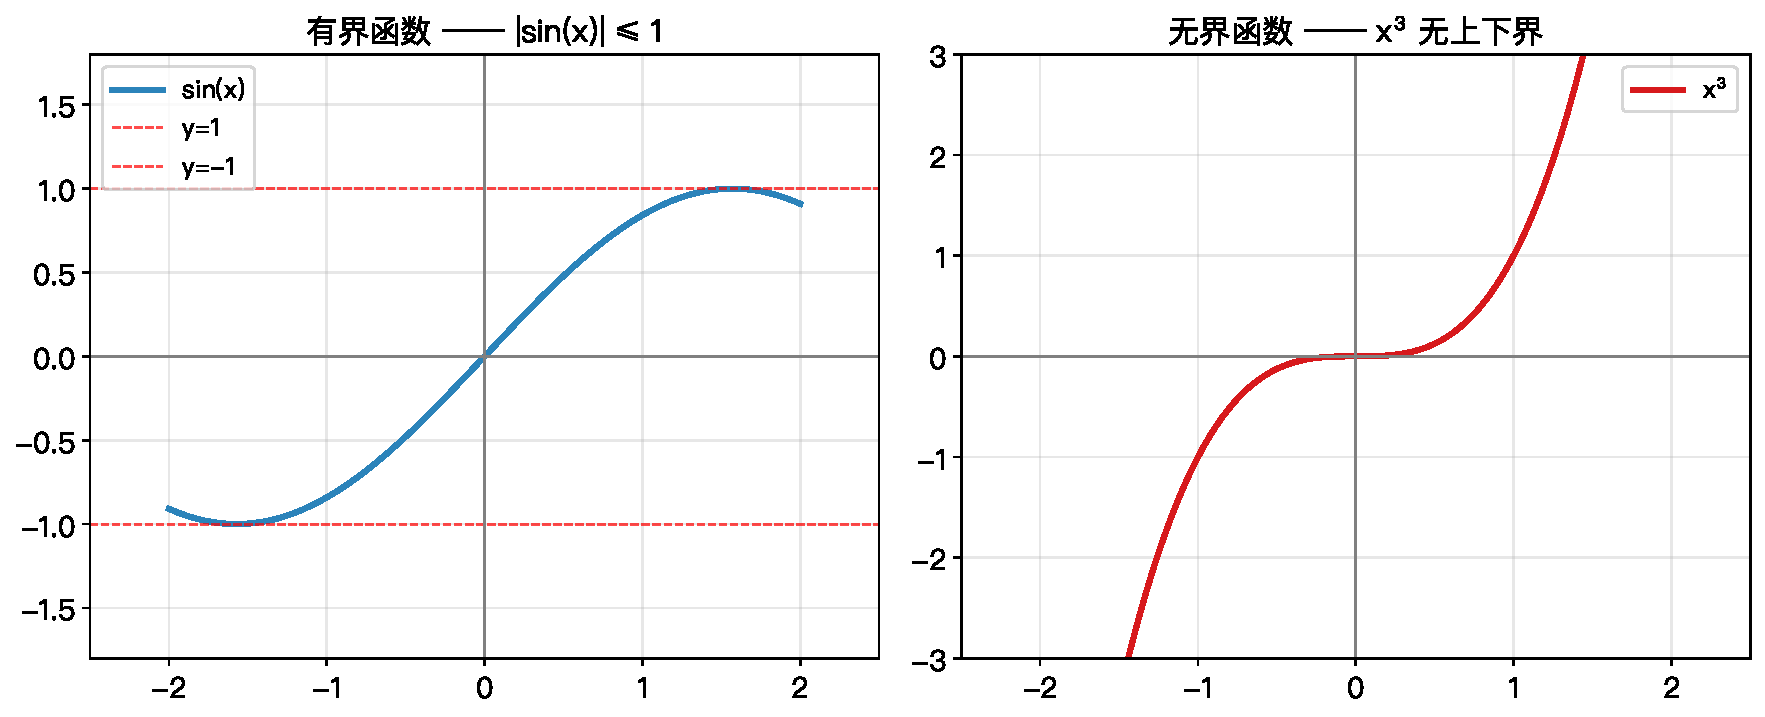
\includegraphics[width=0.85\textwidth]{figures/ch08_bounded.pdf}
\end{center}

\textbf{左图}（\(\sin x\)）：\(|\sin x| \le 1\)——有界函数，上下界为 \(\pm 1\)。\\
\textbf{右图}（\(x^3\)）：没有实数 \(M\) 能限制它——无界函数。

\textbf{常见有界函数：} \(\sin x\)、\(\cos x\)、\(\arctan x\)、常数函数

\textbf{常见无界函数：} \(x^n\)、\(a^x\)、\(\log_a x\)、\(\tan x\)
\end{examplebox}


% ============================================================
\section{复合函数——函数的函数}
% ============================================================

\begin{definitionbox}[复合函数]
如果 \(y = f(u)\)，且 \(u = g(x)\)，那么
\[
y = f(g(x))
\]
称为 \(f\) 和 \(g\) 的\textbf{复合函数}（读作 f of g of x）。

其中 \(g\) 是\textbf{内层函数}，\(f\) 是\textbf{外层函数}。
\end{definitionbox}

\begin{examplebox}[6——复合函数的例子]
\[
f(u) = \sqrt{u},\quad g(x) = 1 - x^2 \;\Longrightarrow\; f(g(x)) = \sqrt{1 - x^2}
\]

从外到内读：\(\sqrt{\;\cdot\;}\) 里面是 \(1 - x^2\)。

\textbf{复合函数的定义域：}
\begin{enumerate}
  \item 先找内层函数 \(g(x)\) 的定义域
  \item 再保证外层函数 \(f(u)\) 的定义域——即 \(g(x)\) 的值必须在 \(f\) 的定义域内
\end{enumerate}

\textbf{例：} \(f(x) = \sqrt{x}\)，\(g(x) = 2x - 1\)，则 \(f(g(x)) = \sqrt{2x - 1}\)。
定义域：\(2x - 1 \ge 0\)，即 \(x \ge 1/2\)。
\end{examplebox}


% ============================================================
\section{反函数——逆对应}
% ============================================================

\begin{definitionbox}[反函数]
如果函数 \(f: D \to R\) 是一一对应的（每个 \(y\) 唯一对应一个 \(x\)），
那么它的\textbf{反函数}（读作 fǎn hán shù）记作 \(f^{-1}\)：
\[
f^{-1}(y) = x \;\Longleftrightarrow\; f(x) = y
\]

\textbf{图像关系：} \(y = f(x)\) 和 \(y = f^{-1}(x)\) 关于直线 \(y = x\) 对称。
\end{definitionbox}

\begin{examplebox}[7——反函数的对称性]
\begin{center}
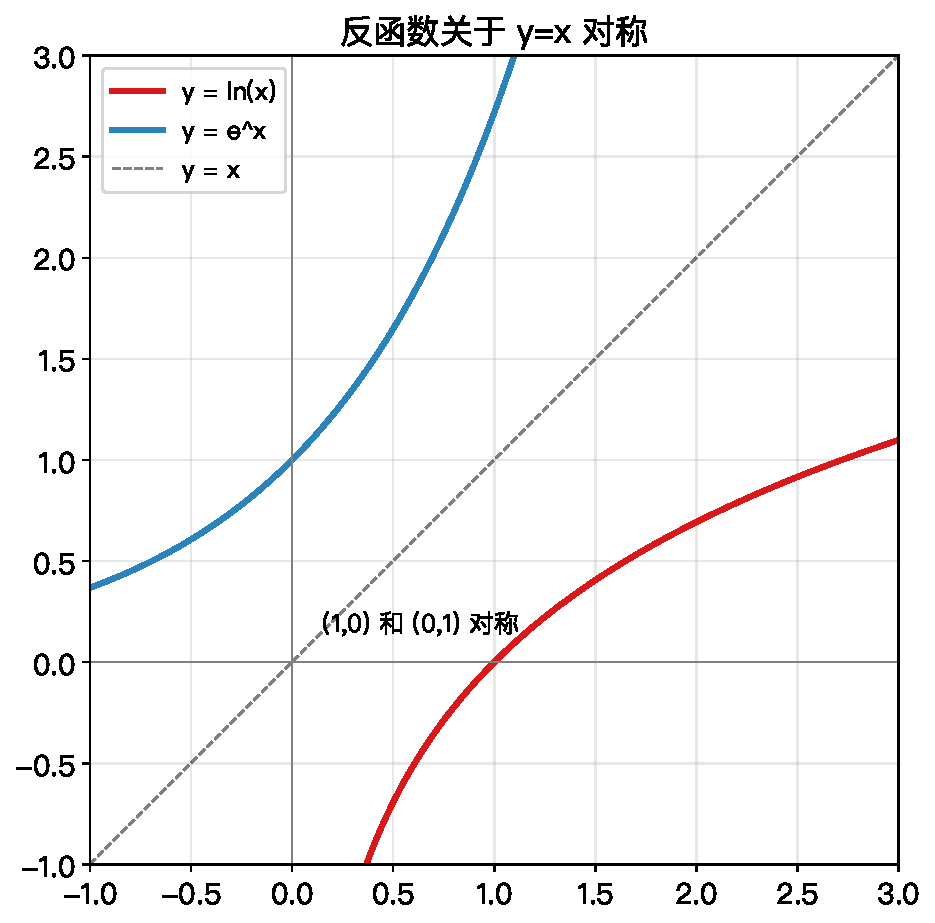
\includegraphics[width=0.5\textwidth]{figures/ch08_inverse_function.pdf}
\end{center}

\textbf{指数和对数是反函数：}
\[
y = e^x \;\Longleftrightarrow\; y = \ln x
\]
\((0,1)\) 在 \(e^x\) 上，\((1,0)\) 在 \(\ln x\) 上——关于 \(y = x\) 对称。

\textbf{另一对反函数：}
\[
y = x^2 \;(x \ge 0) \;\Longleftrightarrow\; y = \sqrt{x}
\]
\end{examplebox}

\begin{notebox}
\textbf{不是所有函数都有反函数！}
只有\textbf{一一对应}的函数才有反函数（即每个 \(y\) 值只对应一个 \(x\) 值）。

例如 \(y = x^2\)（定义域为 \(\mathbb{R}\)）没有反函数，因为 \(y=4\) 对应 \(x=2\) 和 \(x=-2\)。
但如果限制定义域为 \(x \ge 0\)，则有反函数 \(y = \sqrt{x}\)。
\end{notebox}


% ============================================================
\section{函数性质在 AI 中的应用}
% ============================================================

\begin{examplebox}[8——激活函数]
AI 中的激活函数需要特定的性质：

\begin{center}
\begin{tabular}{c|c|c}
\textbf{激活函数} & \textbf{数学形式} & \textbf{关键性质} \\
\hline
Sigmoid & \(\sigma(x) = \dfrac{1}{1 + e^{-x}}\) & 有界 \((0,1)\)，单调递增 \\
ReLU & \(\text{ReLU}(x) = \max(0, x)\) & 无上界，单调递增 \\
Tanh & \(\tanh x = \dfrac{e^x - e^{-x}}{e^x + e^{-x}}\) & 有界 \((-1,1)\)，奇函数 \\
\end{tabular}
\end{center}

\textbf{为什么需要这些性质？}
\begin{itemize}
  \item 有界性：把输出限制在特定范围（如概率在 0 到 1 之间）
  \item 单调性：保证梯度方向一致，训练更稳定
  \item 奇函数：某些情况下加速收敛（Tanh 比 Sigmoid 快）
\end{itemize}
\end{examplebox}


% ============================================================
\section{第0编总回顾——函数基础重建完成！}
% ============================================================

八章、从零开始，你走过了这样一条路：

\begin{center}
\fcolorbox{blue!40}{blue!5}{\parbox{0.9\textwidth}{
\textbf{\large 第0编 · 函数基础重建 · 路线图}

\[
\begin{array}{c}
\text{第1章 函数的概念（什么是函数？）} \\
\downarrow \\
\text{第2章 函数的图像（把函数画出来）} \\
\downarrow \\
\text{第3章 幂函数与多项式（幂的增长）} \\
\downarrow \\
\text{第4章 指数函数（指数增长）} \\
\downarrow \\
\text{第5章 对数函数（指数的逆）} \\
\downarrow \\
\text{第6-7章 三角函数（周期运动）} \\
\downarrow \\
\text{第8章 四大性质 + 复合与反函数（系统化总结）}
\end{array}
\]
}}
\end{center}

你不再是从零开始的初学者——你已经掌握了数学分析所需要的\textbf{全部预备知识}。


% ============================================================
\section{符号卡片}
% ============================================================

\begin{symbolcard}
单调递增 & —— & \(x_1 < x_2 \Rightarrow f(x_1) < f(x_2)\) \\
单调递减 & —— & \(x_1 < x_2 \Rightarrow f(x_1) > f(x_2)\) \\
奇函数 \(f(-x) = -f(x)\) & \verb|f(-x) = -f(x)| & 关于原点对称 \\
偶函数 \(f(-x) = f(x)\) & \verb|f(-x) = f(x)| & 关于 \(y\) 轴对称 \\
周期 \(T\) & —— & \(f(x + T) = f(x)\) \\
有界 \(|f(x)| \le M\) & —— & 存在常数 \(M\) 控制函数值 \\
\(f(g(x))\) & \verb|f(g(x))| & 复合函数，g 在内 f 在外 \\
\(f^{-1}(x)\) & \verb|f^{-1}(x)| & 反函数，与 \(f\) 关于 \(y=x\) 对称 \\
\end{symbolcard}


% ============================================================
\section{代码验证}
% ============================================================

\begin{lstlisting}[caption=函数性质的数值验证]
import numpy as np

# 1. 验证奇偶性
print("=== 奇偶性验证 ===")
def check_parity(f, name, xs):
    is_odd = all(abs(f(-x) + f(x)) < 1e-10 for x in xs)
    is_even = all(abs(f(-x) - f(x)) < 1e-10 for x in xs)
    if is_odd: print(f"  {name}: 奇函数")
    elif is_even: print(f"  {name}: 偶函数")
    else: print(f"  {name}: 非奇非偶")

xs = np.linspace(0.1, 5, 20)
check_parity(lambda x: x**3, "x^3", xs)
check_parity(lambda x: x**2, "x^2", xs)
check_parity(lambda x: np.sin(x), "sin(x)", xs)
check_parity(lambda x: np.cos(x), "cos(x)", xs)
check_parity(lambda x: 2**x, "2^x", xs)

print()

# 2. 验证周期性
print("=== 周期性验证 ===")
for T in [2*np.pi, np.pi]:
    x = 0.5
    print(f"  sin(x+{T:.2f}) = {np.sin(x+T):.4f}, sin(x) = {np.sin(x):.4f}")

print()

# 3. 验证有界性
print("=== 有界性验证 ===")
print(f"  sin(x) 的最大值: {np.max(np.sin(np.linspace(0, 100, 10000))):.4f}")
print(f"  sin(x) 的最小值: {np.min(np.sin(np.linspace(0, 100, 10000))):.4f}")
print(f"  arctan(x) 的最大值: {np.arctan(1e6):.4f}")
print(f"  arctan(x) 的最小值: {np.arctan(-1e6):.4f}")

print()

# 4. 验证反函数关系
print("=== 反函数验证 ===")
for x in [0.5, 1, 2, 3]:
    exp_val = np.exp(x)
    log_val = np.log(exp_val)
    print(f"  e^{x:.1f} = {exp_val:.4f}, ln(e^{x:.1f}) = {log_val:.4f}")
\end{lstlisting}

运行结果：
\begin{lstlisting}[frame=none,backgroundcolor={},numbers=none]
=== 奇偶性验证 ===
  x^3: 奇函数
  x^2: 偶函数
  sin(x): 奇函数
  cos(x): 偶函数
  2^x: 非奇非偶

=== 周期性验证 ===
  sin(x+6.28) = 0.4794, sin(x) = 0.4794
  sin(x+3.14) = -0.4794, sin(x) = 0.4794

=== 有界性验证 ===
  sin(x) 的最大值: 0.9999
  sin(x) 的最小值: -0.9999
  arctan(x) 的最大值: 1.5708
  arctan(x) 的最小值: -1.5708

=== 反函数验证 ===
  e^0.5 = 1.6487, ln(e^0.5) = 0.5000
  e^1.0 = 2.7183, ln(e^1.0) = 1.0000
  e^2.0 = 7.3891, ln(e^2.0) = 2.0000
  e^3.0 = 20.0855, ln(e^3.0) = 3.0000
\end{lstlisting}


% ============================================================
\section{本章小结}
% ============================================================

\begin{progressbox}
\textbf{四大性质：}
\begin{itemize}
  \item 单调性：递增 \((x_1 < x_2 \Rightarrow f(x_1) < f(x_2))\) 或递减
  \item 奇偶性：奇 \((f(-x) = -f(x))\)、偶 \((f(-x) = f(x))\)、或非奇非偶
  \item 周期性：\(f(x + T) = f(x)\)，常见周期 \(2\pi, \pi\)
  \item 有界性：存在 \(M\) 使 \(|f(x)| \le M\)
\end{itemize}

\textbf{复合函数：} \(f(g(x))\)——从内到外逐层计算

\textbf{反函数：} \(f^{-1}\)——关于 \(y = x\) 对称，只有一一对应才有反函数
\end{progressbox}

\subsection*{通往第一编——数列极限}

\textbf{第0编到此结束！} 你完成了函数基础重建的全部 8 章。

\textbf{第一编}我们将进入数学分析的核心——\textbf{数列极限}。
这是你第一次接触"无限"和"趋近"的严格数学语言。
准备好了吗？我们开始。


% ============================================================
% 习题
% ============================================================
\section{习题}

% ===== 送分 =====

\begin{exercise}[0]
判断 \(f(x) = x + 1\) 是单调递增还是递减？
\end{exercise}

\begin{exercise}[0]
判断 \(f(x) = 3\) 是奇函数、偶函数、还是非奇非偶？
\end{exercise}

\begin{exercise}[0]
\(\sin x\) 的周期是多少？\(\tan x\) 的周期是多少？
\end{exercise}

\begin{exercise}[0]
判断 \(f(x) = \arctan x\) 是有界函数还是无界函数？
\end{exercise}

% ===== 简单 =====

\begin{exercise}[1]
证明 \(f(x) = 3x - 2\) 是单调递增函数。
\end{exercise}

\begin{exercise}[1]
判断奇偶性：
\[
(1)\; f(x) = x^4 + 1 \qquad
(2)\; f(x) = x^3 + x \qquad
(3)\; f(x) = 2^x \qquad
(4)\; f(x) = |x|
\]
\end{exercise}

\begin{exercise}[1]
已知 \(f(x) = x^2\)，\(g(x) = 2x + 1\)，求 \(f(g(1))\) 和 \(g(f(1))\)。
\end{exercise}

\begin{exercise}[1]
\(y = \ln x\) 的反函数是什么？\(y = e^x\) 的反函数呢？
\end{exercise}

% ===== 基础 =====

\begin{exercise}[2]
求复合函数 \(f(g(x))\) 及其定义域：
\[
(1)\; f(x) = \sqrt{x},\; g(x) = x - 3 \qquad
(2)\; f(x) = \frac{1}{x},\; g(x) = x + 2
\]
\end{exercise}

\begin{exercise}[2]
证明 \(f(x) = x^2 + 1\) 在 \((-\infty, 0]\) 上单调递减，在 \([0, \infty)\) 上单调递增。
\end{exercise}

\begin{exercise}[2]
求下列函数的值域，并判断是否有界：
\[
(1)\; f(x) = \sin x - 1 \qquad (2)\; f(x) = e^{-x^2} \qquad (3)\; f(x) = \frac{1}{x}
\]
\end{exercise}

\begin{exercise}[2]
求函数 \(y = \sin(2x + \pi/3)\) 的周期、振幅、初相。
\end{exercise}

% ===== 普通 =====

\begin{exercise}[3]
已知 \(f(x) = 
\begin{cases}
x^2, & x \ge 0 \\
-x,  & x < 0
\end{cases}\)，判断 \(f(x)\) 的奇偶性。
\end{exercise}

\begin{exercise}[3]
已知 \(f(x) = \ln(x + \sqrt{1 + x^2})\)，证明 \(f(x)\) 是奇函数。
\end{exercise}

\begin{exercise}[3]
求下列函数的反函数：
\[
(1)\; f(x) = 3x + 2 \qquad (2)\; f(x) = \frac{x - 1}{x + 1} \;(x \neq -1)
\]
\end{exercise}

\begin{exercise}[3]
已知 \(f(x) = e^x\)，\(g(x) = \sin x\)，求 \(f(g(x))\) 和 \(g(f(x))\)，并说明它们分别是什么函数（幂/指/对/三角/复合）？
\end{exercise}

\begin{exercise}[3]
已知函数 \(f(x) = \log_2 (x^2 + 1)\)。
\begin{enumerate}
  \item[(1)] 求定义域
  \item[(2)] 判断奇偶性
  \item[(3)] 求值域（提示：\(x^2 + 1 \ge 1\)，所以 \(\log_2(x^2+1) \ge 0\)）
\end{enumerate}
\end{exercise}

% ===== 中等 =====

\begin{exercise}[4]
已知 \(f(x) = \dfrac{2^x - 2^{-x}}{2}\)（这其实是 \(\sinh x\)，双曲正弦）。
\begin{enumerate}
  \item[(1)] 判断奇偶性
  \item[(2)] 证明 \(f\) 是单调递增的
  \item[(3)] 求 \(f\) 的值域
\end{enumerate}
\end{exercise}

\begin{exercise}[4]
已知 \(f(x) = x^2 - 4x + 5\)。
\begin{enumerate}
  \item[(1)] 配方法写成 \(f(x) = (x - a)^2 + b\) 的形式
  \item[(2)] 判断单调区间（在哪个区间递增？哪个区间递减？）
  \item[(3)] 求最小值
\end{enumerate}
\end{exercise}

\begin{exercise}[4]
求函数 \(f(x) = \sqrt{1 - \sin^2 x}\) 的周期（提示：先化简）。
\end{exercise}

\begin{exercise}[4]
设 \(f(x) = \dfrac{1}{1 + e^{-x}}\)（Sigmoid 函数）。
\begin{enumerate}
  \item[(1)] 证明 \(f\) 是单调递增的
  \item[(2)] 证明 \(0 < f(x) < 1\)
  \item[(3)] 求 \(\lim_{x \to \infty} f(x)\) 和 \(\lim_{x \to -\infty} f(x)\)
\end{enumerate}
\end{exercise}

\begin{exercise}[4]
已知 \(f(x) = x^2 - 2x\)，\(g(x) = x + 1\)。
\begin{enumerate}
  \item[(1)] 求 \(f(g(x))\) 和 \(g(f(x))\)
  \item[(2)] 解方程 \(f(g(x)) = g(f(x))\)
\end{enumerate}
\end{exercise}

% ===== 进阶 =====

\begin{exercise}[5]
已知 \(f(x)\) 是奇函数，\(g(x)\) 是偶函数，且 \(f(x) + g(x) = e^x\)。
\begin{enumerate}
  \item[(1)] 用 \(x\) 替换为 \(-x\) 得到另一个方程
  \item[(2)] 联立解出 \(f(x)\) 和 \(g(x)\) 的表达式
\end{enumerate}
（提示：利用奇偶性：\(f(-x) = -f(x)\)，\(g(-x) = g(x)\)）
\end{exercise}

\begin{exercise}[5]
证明：若 \(f\) 和 \(g\) 都是单调递增函数，则 \(f(g(x))\) 也是单调递增函数。
\end{exercise}

\begin{exercise}[5]
求函数 \(y = \arctan \dfrac{1}{x}\)（\(x \neq 0\)）的值域。
\end{exercise}

\begin{exercise}[5]
已知 \(f(x) = \log_a (2 - ax)\)（\(a > 0, a \neq 1\)）在 \([0, 1]\) 上单调递减，求 \(a\) 的取值范围。
\end{exercise}

% ===== 拔高 =====

\begin{exercise}[6]
已知函数 \(f(x) = |x - 1| + 2|x - 2| + 3|x - 3|\)。
\begin{enumerate}
  \item[(1)] 去掉绝对值，写成分段函数
  \item[(2)] 求每个分段区间上的单调性
  \item[(3)] 求最小值
\end{enumerate}
\end{exercise}

\begin{exercise}[6]
求证：定义在 \(\mathbb{R}\) 上的任意函数 \(f(x)\) 都可以写成
一个奇函数和一个偶函数的和。
（提示：令 \(g(x) = \dfrac{f(x) + f(-x)}{2}\)，\(h(x) = \dfrac{f(x) - f(-x)}{2}\)）
\end{exercise}

\begin{exercise}[6]
已知函数 \(f(x)\) 满足 \(f(x + y) = f(x) + f(y)\) 对所有 \(x, y\) 成立。
\begin{enumerate}
  \item[(1)] 证明 \(f\) 是奇函数
  \item[(2)] 如果 \(f(1) = 2\)，求 \(f(5)\) 和 \(f(-3)\)
\end{enumerate}
\end{exercise}

% ===== 极难 =====

\begin{exercise}[7]
函数 \(f: \mathbb{R} \to \mathbb{R}\) 满足：
\[
f(x + y) + f(x - y) = 2f(x)\cos y \quad \text{对所有 } x, y \in \mathbb{R} \text{ 成立}
\]
\begin{enumerate}
  \item[(1)] 令 \(y = 0\)，求 \(f(0)\)
  \item[(2)] 令 \(x = 0\)，证明 \(f\) 是偶函数
  \item[(3)] 令 \(x = \pi/2\)，证明 \(f\) 是周期函数
  \item[(4)] 结合 \(f(\pi/2) = 1\)，求 \(f(0)\)、\(f(\pi)\)、\(f(2\pi)\)
\end{enumerate}

\textbf{说明：} 这道题是函数方程与函数性质的综合——从给定的方程中，
一步步推导出函数的奇偶性、周期性、特殊值。
这是数学分析中"由性质确定函数"的一个经典范例。
\end{exercise}

% 第〇编结束，进入第一编

% ============================================================
% 第一编：数列极限
\part{数列极限——从有限到无限的第一步}
% ============================================================
% 第9章：数列的概念——从离散到无限
% ============================================================

\chapter{数列的概念——从离散到无限}

\begin{applicationbox}
\textbf{学完本章你能做什么？}
\begin{enumerate}
  \item 理解\textbf{数列}是什么——按顺序排列的一列数，是离散版本的函数
  \item 掌握\textbf{等差数列}和\textbf{等比数列}的通项与求和
  \item 学会用\textbf{递推公式}表示数列，并推导通项
  \item 判断数列的\textbf{单调性}和\textbf{有界性}——为极限学习做准备
\end{enumerate}
\end{applicationbox}


% ============================================================
\section{从函数到数列——连续 vs 离散}
% ============================================================

前8章我们学的函数，自变量 \(x\) 可以在实数范围内连续变化（取任意值）。

但现实中有很多情况，自变量只能取\textbf{正整数}：

\begin{itemize}
  \item 第1天存 100 元，第2天存 200 元，第3天存 300 元……
  \item 第1代细菌有 1 个，第2代有 2 个，第3代有 4 个……
  \item 第1个月还款 5000 元，第2个月还款 4980 元，第3个月还款 4960 元……
\end{itemize}

这些按\textbf{顺序排列}的一列数，就叫\textbf{数列}。

\begin{center}
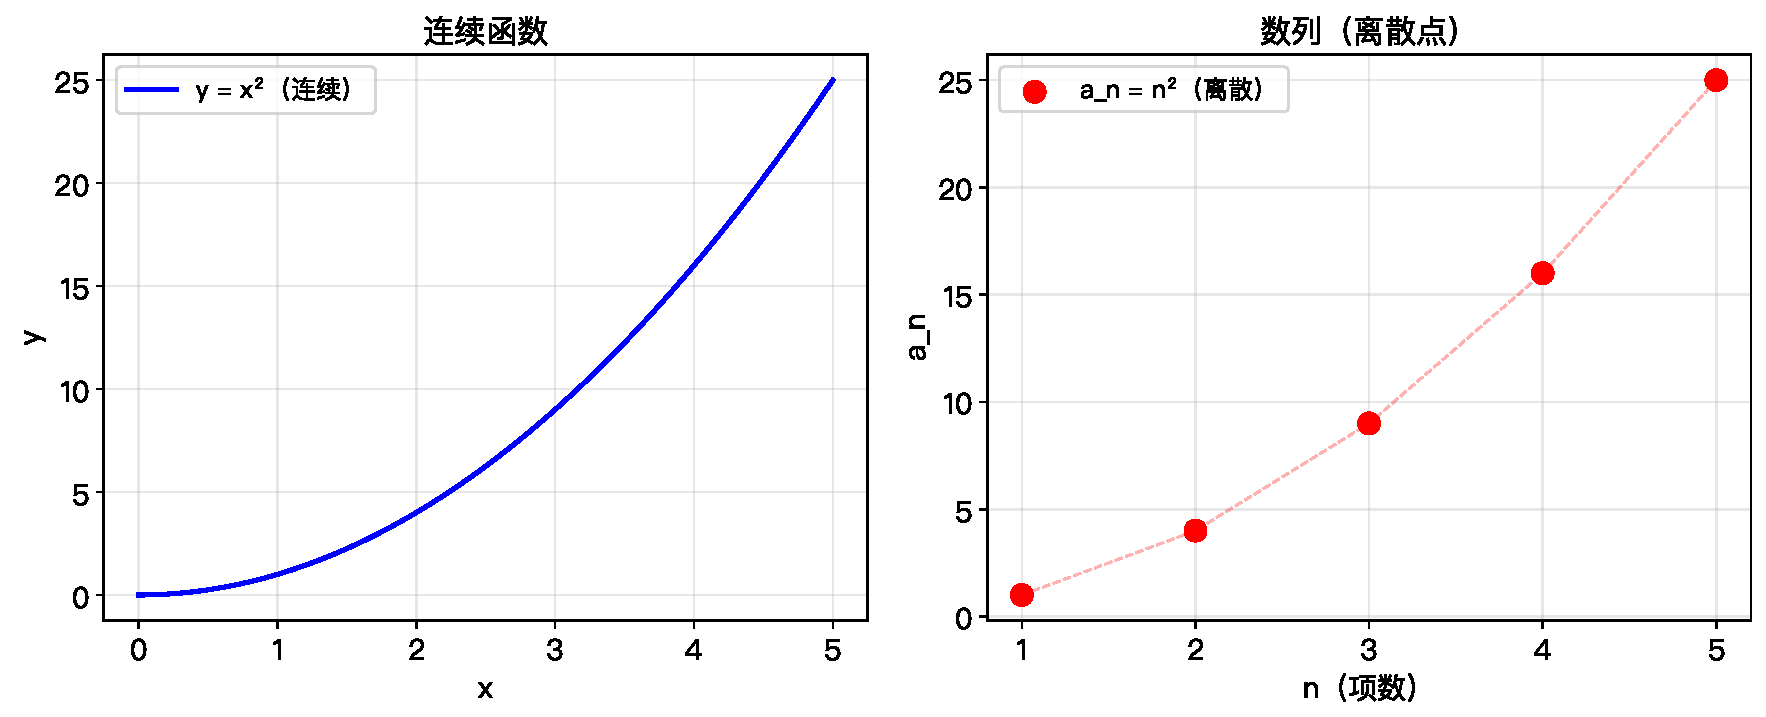
\includegraphics[width=0.8\textwidth]{figures/ch09_continuous_vs_discrete.pdf}
\end{center}

左边是连续函数 \(y = x^2\)，右边是离散数列 \(a_n = n^2\)——同样的公式，但数列只取正整数点。


% ============================================================
\section{数列的定义}
% ============================================================

\begin{definitionbox}[数列]
按一定顺序排列的一列数称为\textbf{数列}（读作 shù liè，英文 sequence）。

记作：
\[
a_1, a_2, a_3, \ldots, a_n, \ldots
\]

其中：
\begin{itemize}
  \item \(a_1\) 是\textbf{第1项}（首项），\(a_n\) 是\textbf{第 \(n\) 项}（通项）
  \item \(n\) 是\textbf{项数}（下标，正整数）
  \item 整个数列简记为 \(\{a_n\}\) 或 \(a_n\)（习惯上混用）
\end{itemize}

\textbf{数列和函数的关系：}
\[
\text{数列 } a_n = f(n) \quad (n = 1, 2, 3, \ldots)
\]
数列就是以\textbf{正整数}为定义域的函数。
\end{definitionbox}

\begin{examplebox}[1——写出数列的前几项]
写出 \(a_n = 2n - 1\) 的前 5 项：

\[
n=1: a_1 = 1,\; n=2: a_2 = 3,\; n=3: a_3 = 5,\; n=4: a_4 = 7,\; n=5: a_5 = 9
\]

所以数列为：\(1, 3, 5, 7, 9, \ldots\)（奇数数列）
\end{examplebox}


% ============================================================
\section{等差数列——均匀变化}
% ============================================================

\begin{definitionbox}[等差数列]
如果数列从第2项起，每一项与前一项的差等于同一个常数，则称该数列为\textbf{等差数列}（读作 děng chā shù liè）。

\[
a_{n+1} - a_n = d \quad (\text{\(d\) 是常数，叫\textbf{公差}})
\]

\textbf{通项公式：}
\[
a_n = a_1 + (n-1)d
\]

\textbf{前 \(n\) 项和：}
\[
S_n = \frac{n(a_1 + a_n)}{2} = na_1 + \frac{n(n-1)}{2}d
\]
\end{definitionbox}

\begin{examplebox}[2——等差数列]
已知等差数列首项 \(a_1 = 3\)，公差 \(d = 2\)。

数列：\(3, 5, 7, 9, 11, \ldots\)

通项：\(a_n = 3 + (n-1) \times 2 = 2n + 1\)

前 5 项和：
\[
S_5 = \frac{5(3 + 11)}{2} = \frac{5 \times 14}{2} = 35
\]

验证：\(3 + 5 + 7 + 9 + 11 = 35\) [OK]
\end{examplebox}

\begin{examplebox}[3——等差数列的应用]
小明第一天背 10 个单词，之后每天比前一天多背 3 个。第 30 天背多少个？

解：\(a_1 = 10\)，\(d = 3\)，\(n = 30\)
\[
a_{30} = 10 + (30-1) \times 3 = 10 + 87 = 97
\]

30 天共背了多少个？
\[
S_{30} = \frac{30(10 + 97)}{2} = 15 \times 107 = 1605
\]
\end{examplebox}


% ============================================================
\section{等比数列——成倍变化}
% ============================================================

\begin{definitionbox}[等比数列]
如果数列从第2项起，每一项与前一项的比等于同一个常数，则称该数列为\textbf{等比数列}（读作 děng bǐ shù liè）。

\[
\frac{a_{n+1}}{a_n} = q \quad (\text{\(q\) 是常数，叫\textbf{公比}，\(q \neq 0\)})
\]

\textbf{通项公式：}
\[
a_n = a_1 q^{n-1}
\]

\textbf{前 \(n\) 项和（\(q \neq 1\)）：}
\[
S_n = a_1 \frac{1 - q^n}{1 - q}
\]
\end{definitionbox}

\begin{examplebox}[4——等比数列 vs 等差数列]
\begin{center}
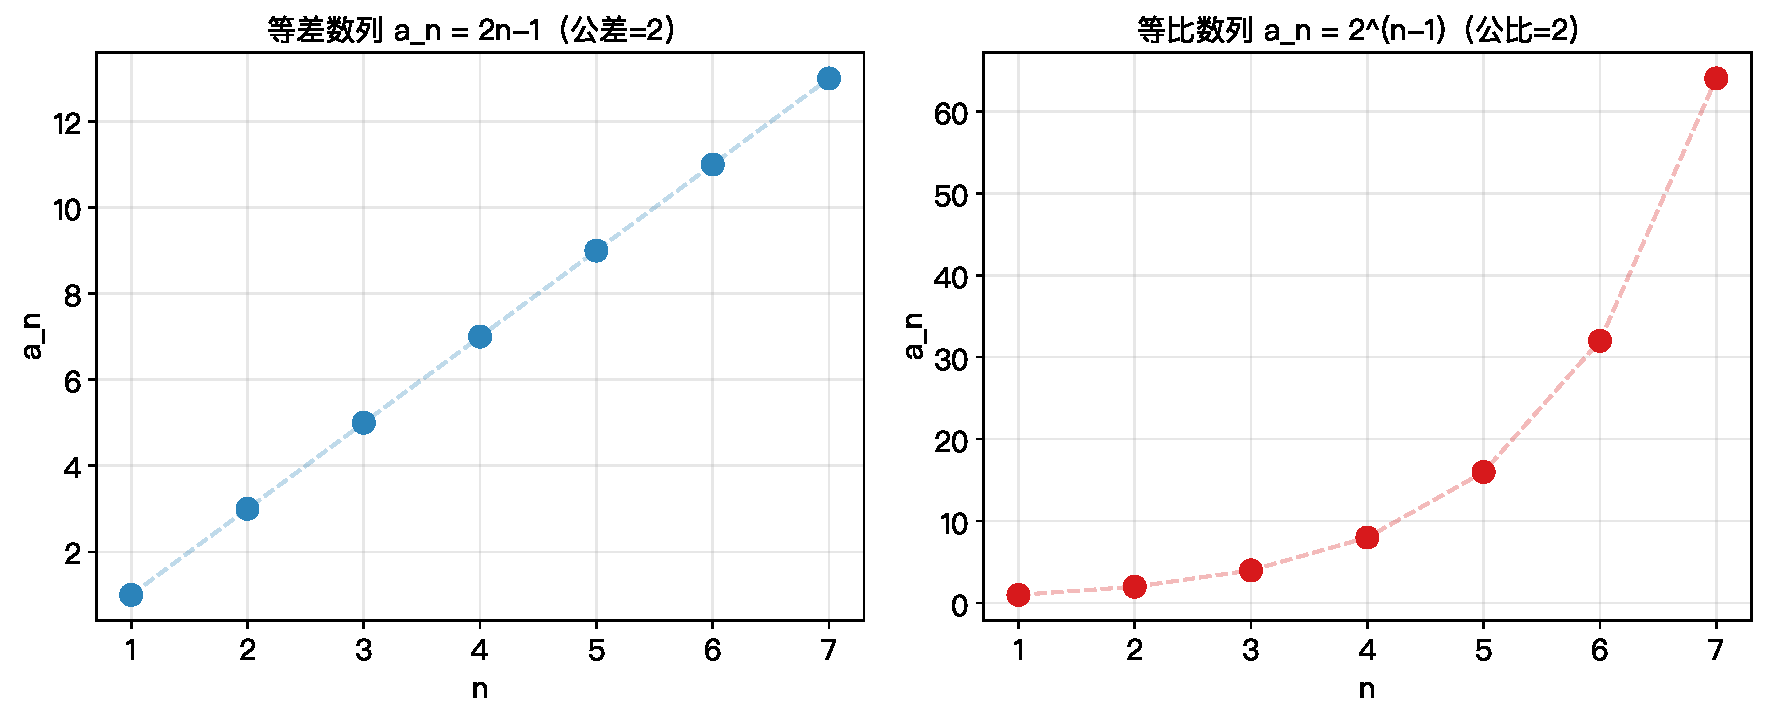
\includegraphics[width=0.85\textwidth]{figures/ch09_arithmetic_geometric.pdf}
\end{center}

\textbf{左图：}等差数列 \(a_n = 2n-1\)——增长是\textbf{均匀}的（每天+2）。\\
\textbf{右图：}等比数列 \(a_n = 2^{n-1}\)——增长越来越\textbf{快}（每天$\times$2）。

\textbf{关键区别：}等差是线性增长，等比是指数增长。
\end{examplebox}

\begin{examplebox}[5——等比数列的应用]
某种细菌每 1 小时分裂一次（数量翻倍）。初始 100 个，8 小时后有多少个？

解：\(a_1 = 100\)，\(q = 2\)，\(n = 8\)
\[
a_8 = 100 \times 2^{8-1} = 100 \times 2^7 = 100 \times 128 = 12800
\]

8 小时内总共产生了多少个（含初始）？
\[
S_8 = 100 \times \frac{1 - 2^8}{1 - 2} = 100 \times \frac{1 - 256}{-1} = 100 \times 255 = 25500
\]
\end{examplebox}


% ============================================================
\section{递推公式——用前一项定义后一项}
% ============================================================

有时候数列没有明确的通项公式，而是通过\textbf{递推关系}定义。

\begin{definitionbox}[递推公式]
如果数列的每一项由前一项（或前几项）通过一个公式确定，这个公式叫\textbf{递推公式}。

常见形式：
\[
a_{n+1} = f(a_n) \quad \text{或} \quad a_{n+1} = p a_n + q
\]
\end{definitionbox}

\begin{examplebox}[6——由递推求通项]
已知 \(a_1 = 1\)，\(a_{n+1} = 2a_n + 1\)，求 \(a_5\)。

\textbf{逐项计算：}
\[
a_1 = 1
\]
\[
a_2 = 2 \times 1 + 1 = 3
\]
\[
a_3 = 2 \times 3 + 1 = 7
\]
\[
a_4 = 2 \times 7 + 1 = 15
\]
\[
a_5 = 2 \times 15 + 1 = 31
\]

数列：\(1, 3, 7, 15, 31, \ldots\)

\textbf{猜想通项：} \(a_n = 2^n - 1\)（验证：\(2^1-1=1\)，\(2^2-1=3\)，\(2^3-1=7\) [OK]）
\end{examplebox}


% ============================================================
\section{数列的单调性与有界性}
% ============================================================

和函数一样，数列也有单调性和有界性——这对后续学习极限至关重要。

\begin{definitionbox}[数列的单调性与有界性]
\textbf{单调递增：} \(a_{n+1} \ge a_n\) 对所有 \(n\) 成立。\\
\textbf{单调递减：} \(a_{n+1} \le a_n\) 对所有 \(n\) 成立。\\
\textbf{有上界：}存在 \(M\) 使得 \(a_n \le M\) 对所有 \(n\) 成立。\\
\textbf{有下界：}存在 \(m\) 使得 \(a_n \ge m\) 对所有 \(n\) 成立。
\end{definitionbox}

\begin{examplebox}[7——单调有界数列]
数列 \(a_n = 1 - \dfrac{1}{n}\)：

\begin{center}
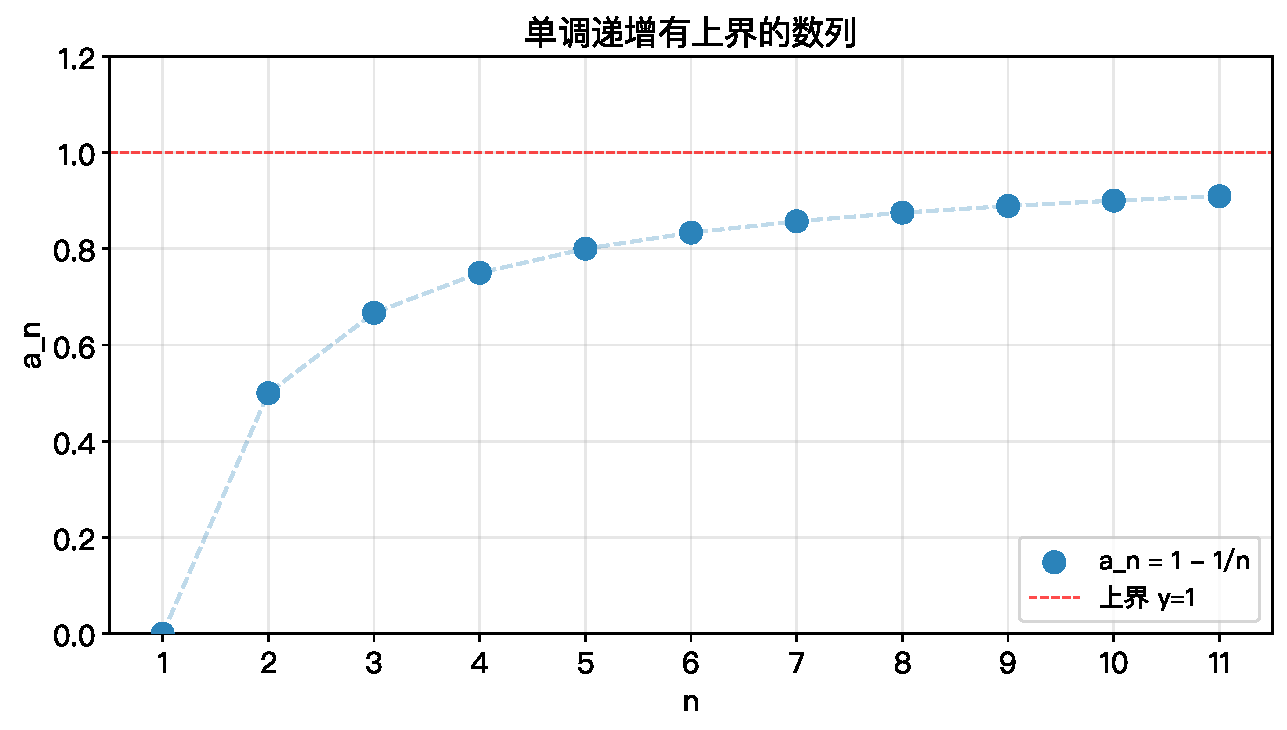
\includegraphics[width=0.75\textwidth]{figures/ch09_monotonic_bounded.pdf}
\end{center}

\textbf{单调性：} \(a_n = 1 - \frac{1}{n}\)，当 \(n\) 增大时 \(\frac{1}{n}\) 减小，所以 \(a_n\) 增大 \(\rightarrow\) \textbf{单调递增}。

\textbf{有界性：} \(a_n < 1\) 对所有 \(n\) 成立（因为 \(\frac{1}{n} > 0\)），所以 1 是\textbf{上界}。\\
同时 \(a_n \ge a_1 = 0\)，0 是\textbf{下界}。\\
\(\rightarrow\) 单调递增有上界（且下界）。
\end{examplebox}

\begin{examplebox}[8——摆动数列]
数列 \(a_n = \dfrac{(-1)^n}{n}\)：

\begin{center}
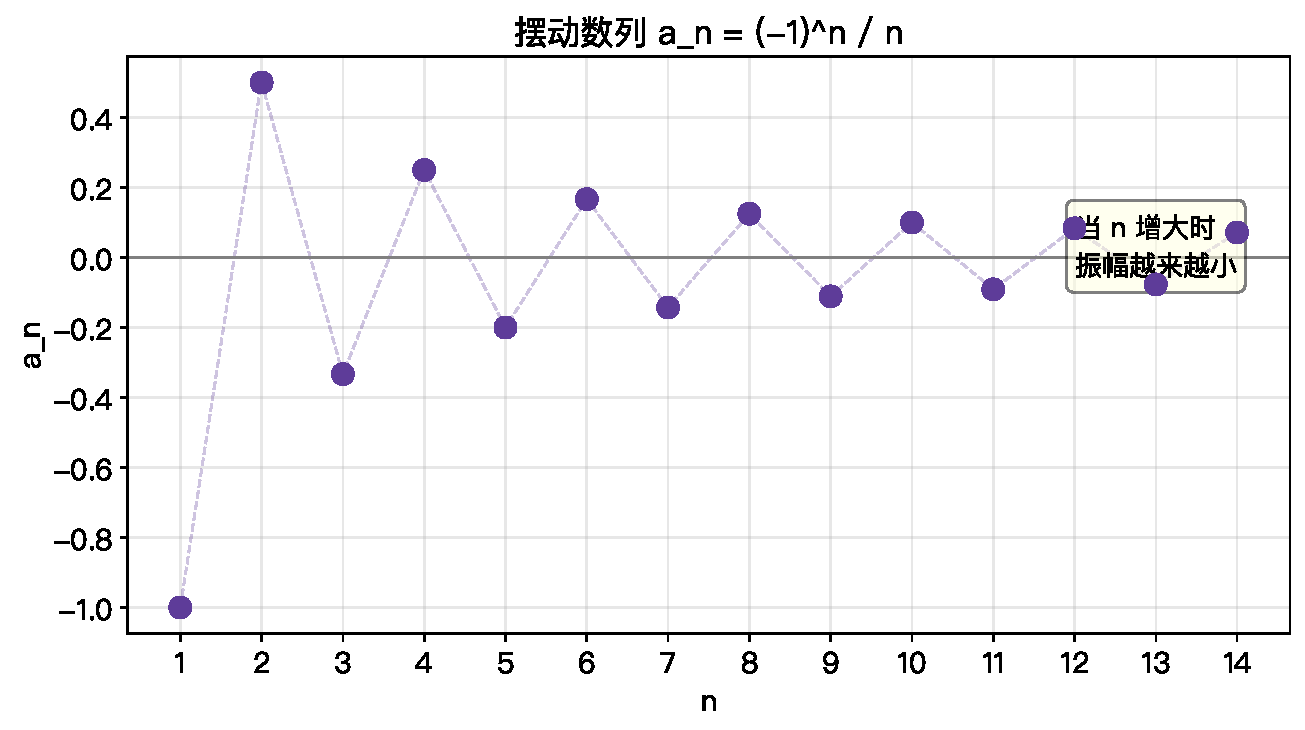
\includegraphics[width=0.75\textwidth]{figures/ch09_oscillating.pdf}
\end{center}

这个数列在正负之间摆动，但\textbf{振幅越来越小}，趋近于 0。\\
它\textbf{不是单调的}，但\textbf{是有界的}（\(-1 \le a_n \le 1\)）。
\end{examplebox}


% ============================================================
\section{符号卡片}
% ============================================================

\begin{symbolcard}
\(\{a_n\}\) & \verb|{a_n}| & 读作"数列 a n" & 数列 \(a_1, a_2, a_3, \ldots\) \\
\(d\) & —— & 读作"公差" & 等差数列中相邻项的差 \\
\(q\) & —— & 读作"公比" & 等比数列中相邻项的比 \\
\(S_n\) & \verb|S_n| & 读作"S n" & 前 \(n\) 项和 \\
\(a_{n+1} = f(a_n)\) & —— & —— & 递推公式 \\
\end{symbolcard}


% ============================================================
\section{代码验证}
% ============================================================

\begin{lstlisting}[caption=数列的数值验证]
import numpy as np

# 1. 等差数列
print("=== 等差数列 a_n = 2n+1 ===")
a1, d = 3, 2
for n in range(1, 9):
    an = a1 + (n-1)*d
    print(f"  a_{n} = {an}", end="")
print()

# 前n项和
S5 = 5*(a1 + (a1+4*d)) // 2
print(f"  S_5 = {S5}")

print()

# 2. 等比数列
print("=== 等比数列 a_n = 2^(n-1) ===")
for n in range(1, 11):
    an = 2**(n-1)
    print(f"  a_{n:2d} = {an:4d}", end="")
print()

# 前n项和
S10 = 1 * (1 - 2**10) / (1 - 2)
print(f"  S_10 = {int(S10)}")

print()

# 3. 递推 a_{n+1} = 2a_n + 1
print("=== 递推数列 a_{n+1} = 2a_n + 1 ===")
a = 1
for n in range(1, 8):
    print(f"  a_{n} = {a}")
    a = 2*a + 1

print()

# 4. 数列单调性判断
print("=== 单调性判断 ===")
def is_increasing(seq):
    return all(seq[i] <= seq[i+1] for i in range(len(seq)-1))

def is_decreasing(seq):
    return all(seq[i] >= seq[i+1] for i in range(len(seq)-1))

seq1 = [1 - 1/n for n in range(1, 20)]  # 递增
seq2 = [1/n for n in range(1, 20)]      # 递减
seq3 = [(-1)**n / n for n in range(1, 20)]  # 摆动

print(f"  a_n = 1-1/n: 递增={is_increasing(seq1)}")
print(f"  a_n = 1/n:   递增={is_increasing(seq2)} 递减={is_decreasing(seq2)}")
print(f"  a_n = (-1)^n/n: 递增={is_increasing(seq3)} 递减={is_decreasing(seq3)}")
\end{lstlisting}


% ============================================================
\section{本章小结}
% ============================================================

\begin{progressbox}
\textbf{数列}：按顺序排列的一列数，\(a_n = f(n)\)，\(n\) 为正整数

\textbf{等差数列}：\(a_{n+1} - a_n = d\)，通项 \(a_n = a_1 + (n-1)d\)

\textbf{等比数列}：\(\dfrac{a_{n+1}}{a_n} = q\)，通项 \(a_n = a_1 q^{n-1}\)

\textbf{递推公式}：用前一项（或几项）定义后一项

\textbf{单调性}：递增（\(a_{n+1} \ge a_n\)）或递减（\(a_{n+1} \le a_n\)）

\textbf{有界性}：存在上下界约束数列的值
\end{progressbox}

\subsection*{通往下一章}

\textbf{这一章}你学会了数列的基础——等差、等比、递推、单调、有界。

\textbf{下一章}我们进入数列极限的\textbf{直观理解}——
当 \(n\) 越来越大时，数列趋近于什么？
这是从"有限"走向"无限"的第一步。


% ============================================================
% 习题
% ============================================================
\section{习题}

% ===== 送分 =====

\begin{exercise}[0]
写出数列 \(a_n = 2n\) 的前 5 项。
\end{exercise}

\begin{exercise}[0]
等差数列 \(1, 3, 5, 7, 9\) 的公差 \(d = ?\)
\end{exercise}

\begin{exercise}[0]
等比数列 \(2, 4, 8, 16, 32\) 的公比 \(q = ?\)
\end{exercise}

\begin{exercise}[0]
判断：数列 \(a_n = \dfrac{1}{n}\) 是递增还是递减？
\end{exercise}

% ===== 简单 =====

\begin{exercise}[1]
已知等差数列 \(a_1 = 5\)，\(d = 3\)，求 \(a_{10}\) 和 \(S_{10}\)。
\end{exercise}

\begin{exercise}[1]
已知等比数列 \(a_1 = 2\)，\(q = 3\)，求 \(a_6\) 和 \(S_6\)。
\end{exercise}

\begin{exercise}[1]
写出递推数列 \(a_1 = 2\)，\(a_{n+1} = a_n + 3\) 的前 5 项，并求通项公式。
\end{exercise}

\begin{exercise}[1]
判断 \(a_n = n^2\) 是否有下界？是否有上界？
\end{exercise}

% ===== 基础 =====

\begin{exercise}[2]
已知等差数列中 \(a_5 = 15\)，\(a_{10} = 30\)，求 \(a_1\) 和 \(d\)。
\end{exercise}

\begin{exercise}[2]
一个等比数列的第 3 项是 18，第 6 项是 486，求公比 \(q\) 和首项 \(a_1\)。
\end{exercise}

\begin{exercise}[2]
求前 100 个正整数的和（利用等差数列求和公式）。
\end{exercise}

\begin{exercise}[2]
已知 \(a_n = 3n - 2\)，判断该数列的单调性，并说明理由。
\end{exercise}

% ===== 普通 =====

\begin{exercise}[3]
某公司第一年利润 100 万，之后每年比上一年增长 10\%（等比增长）。
\begin{enumerate}
  \item[(1)] 写出第 \(n\) 年利润的表达式
  \item[(2)] 第 5 年利润是多少（保留整数）？
  \item[(3)] 前 5 年总利润是多少？
\end{enumerate}
\end{exercise}

\begin{exercise}[3]
已知 \(a_1 = 1\)，\(a_{n+1} = 3a_n - 1\)，求 \(a_1\) 到 \(a_5\)，并猜想通项公式。
\end{exercise}

\begin{exercise}[3]
等差数列 \(\{a_n\}\) 中，已知 \(a_3 + a_7 = 20\)，求 \(a_5\)。
（提示：利用等差数列的性质 \(a_m + a_n = 2a_{(m+n)/2}\)）
\end{exercise}

\begin{exercise}[3]
求 \(1 + \dfrac{1}{2} + \dfrac{1}{4} + \dfrac{1}{8} + \cdots + \dfrac{1}{2^{10}}\) 的值。
\end{exercise}

\begin{exercise}[3]
判断数列 \(a_n = \dfrac{n}{n+1}\) 的单调性和有界性，并求它的上界。
\end{exercise}

% ===== 中等 =====

\begin{exercise}[4]
设 \(\{a_n\}\) 是等差数列，\(a_1 = 2\)，\(a_1 + a_3 + a_5 = 18\)，求 \(a_n\) 的通项公式。
\end{exercise}

\begin{exercise}[4]
在等比数列 \(\{a_n\}\) 中，\(a_2 = 6\)，\(a_5 = 48\)，求 \(a_{10}\)。
\end{exercise}

\begin{exercise}[4]
已知 \(a_1 = 2\)，\(a_{n+1} = \dfrac{a_n + 2}{a_n + 1}\)，求 \(a_2, a_3, a_4\)，观察规律。
\end{exercise}

\begin{exercise}[4]
数列 \(\{a_n\}\) 前 \(n\) 项和 \(S_n = n^2 + n\)，求通项 \(a_n\)。
（提示：\(a_n = S_n - S_{n-1}\)，\(n \ge 2\)）
\end{exercise}

\begin{exercise}[4]
证明：若 \(a_{n+1} - a_n\) 是常数，则 \(\{a_n\}\) 是等差数列。
\end{exercise}

% ===== 进阶 =====

\begin{exercise}[5]
已知数列 \(\{a_n\}\) 满足 \(a_1 = \dfrac{1}{2}\)，\(a_{n+1} = \dfrac{a_n}{1 + 2a_n}\)。
\begin{enumerate}
  \item[(1)] 求 \(a_2, a_3, a_4\)
  \item[(2)] 令 \(b_n = \dfrac{1}{a_n}\)，证明 \(\{b_n\}\) 是等差数列
  \item[(3)] 求 \(\{a_n\}\) 的通项公式
\end{enumerate}
\end{exercise}

\begin{exercise}[5]
等差数列 \(\{a_n\}\) 和 \(\{b_n\}\) 的前 \(n\) 项和分别为 \(S_n\) 和 \(T_n\)，
且 \(\dfrac{S_n}{T_n} = \dfrac{2n}{3n+1}\)，求 \(\dfrac{a_5}{b_5}\)。
\end{exercise}

\begin{exercise}[5]
已知 \(a_1 = 1\)，\(a_{n+1} = 2a_n + 3\)，通过构造等比数列求通项。
（提示：设 \(a_{n+1} + k = 2(a_n + k)\)，解出 \(k\)）
\end{exercise}

\begin{exercise}[5]
求证：数列 \(a_n = \dfrac{1}{n} - \dfrac{1}{n+1}\) 的前 \(n\) 项和为 \(S_n = 1 - \dfrac{1}{n+1}\)。
（提示：写出前几项观察规律——裂项相消）
\end{exercise}

% ===== 拔高 =====

\begin{exercise}[6]
已知数列 \(\{a_n\}\)：\(a_1 = 1\)，\(a_{n+1} = \dfrac{2a_n}{a_n + 2}\)。
\begin{enumerate}
  \item[(1)] 求 \(a_2, a_3, a_4\)
  \item[(2)] 求证数列 \(\{\dfrac{1}{a_n}\}\) 是等差数列
  \item[(3)] 求通项公式
\end{enumerate}
\end{exercise}

\begin{exercise}[6]
数列 \(\{a_n\}\) 满足 \(a_1 = 1\)，\(a_{n+1} = \sqrt{a_n^2 + 1}\)。
\begin{enumerate}
  \item[(1)] 求 \(a_2, a_3, a_4\)
  \item[(2)] 猜想通项公式（提示：\(\sqrt{2}, \sqrt{3}, \sqrt{4}\) 的形式）
\end{enumerate}
\end{exercise}

\begin{exercise}[6]
已知 \(S_n = 2a_n - 2\)（\(S_n\) 是前 \(n\) 项和），求通项 \(a_n\)。
（提示：利用 \(S_n - S_{n-1} = a_n\) 得到递推关系）
\end{exercise}

% ===== 极难 =====

\begin{exercise}[7]
已知数列 \(\{a_n\}\) 满足 \(a_1 = 2\)，\(a_{n+1} = \dfrac{a_n^2 + 2}{2a_n}\)。
\begin{enumerate}
  \item[(1)] 求 \(a_2, a_3, a_4\)（保留分数形式）
  \item[(2)] 观察规律，猜想通项公式
  \item[(3)] 证明 \(a_n > \sqrt{2}\) 且 \(\{a_n\}\) 单调递减
\end{enumerate}

\textbf{说明：} 这个数列会\textbf{逼近} \(\sqrt{2}\)——它就是牛顿法求 \(\sqrt{2}\) 的迭代公式。
这已经接近极限的思想了：数列的项越来越接近一个数。
\end{exercise}

% ============================================================
% 第10章：数列极限的直观——趋近一个数的感觉
% ============================================================

\chapter{数列极限的直观——趋近一个数的感觉}

\begin{applicationbox}
\textbf{学完本章你能做什么？}
\begin{enumerate}
  \item 建立数列极限的\textbf{直观概念}——什么是"趋近"？
  \item 区分\textbf{收敛数列}（有极限）和\textbf{发散数列}（没有极限）
  \item 理解极限的"\textbf{ε 带}"几何意义——为下一章的严格定义做准备
\end{enumerate}
\end{applicationbox}


% ============================================================
\section{从第9章来——数列的项在"变化"}
% ============================================================

第9章我们学了数列——\(a_1, a_2, a_3, \ldots, a_n, \ldots\)

当 \(n\) 越来越大时，数列的项会怎么变化？

\begin{center}
\begin{tabular}{c|c|c}
\textbf{数列} & \textbf{当 \(n\) 很大时的行为} & \textbf{结论} \\
\hline
\(a_n = 1/n\) & 越来越接近 0 & \textbf{收敛}到 0 \\
\(a_n = n/(n+1)\) & 越来越接近 1 & \textbf{收敛}到 1 \\
\(a_n = 2^n\) & 越来越大，没有上限 & \textbf{发散}到无穷大 \\
\(a_n = (-1)^n\) & 在 -1 和 1 之间来回跳 & \textbf{发散}（振荡） \\
\end{tabular}
\end{center}

\textbf{极限}研究的就是：当 \(n\) 无限增大时，数列趋近于什么？


% ============================================================
\section{极限的直观概念}
% ============================================================

\begin{definitionbox}[极限的直观定义]
如果当 \(n\) 越来越大时，\(a_n\) 无限趋近于一个固定的数 \(L\)，
那么称 \(L\) 是数列 \(\{a_n\}\) 的\textbf{极限}（读作 jí xiàn，英文 limit）。

记作：
\[
\lim_{n \to \infty} a_n = L
\]

读作："当 \(n\) 趋向于无穷大时，\(a_n\) 的极限等于 \(L\)"。
\end{definitionbox}

\begin{examplebox}[1——从数字中感受极限]
数列 \(a_n = 1/n\)：

\[
a_1 = 1,\; a_2 = 0.5,\; a_3 \approx 0.333,\; a_4 = 0.25,\; a_5 = 0.2
\]
\[
a_{10} = 0.1,\; a_{100} = 0.01,\; a_{1000} = 0.001,\; a_{10000} = 0.0001
\]

\textbf{感受：} \(n\) 每扩大 10 倍，\(a_n\) 缩小到原来的 1/10。\\
当 \(n\) 无限大时，\(a_n\) 无限接近 0——所以 \(\lim_{n \to \infty} \dfrac{1}{n} = 0\)。
\end{examplebox}


% ============================================================
\section{收敛数列——有极限}
% ============================================================

\begin{examplebox}[2——收敛的例子]
\begin{center}
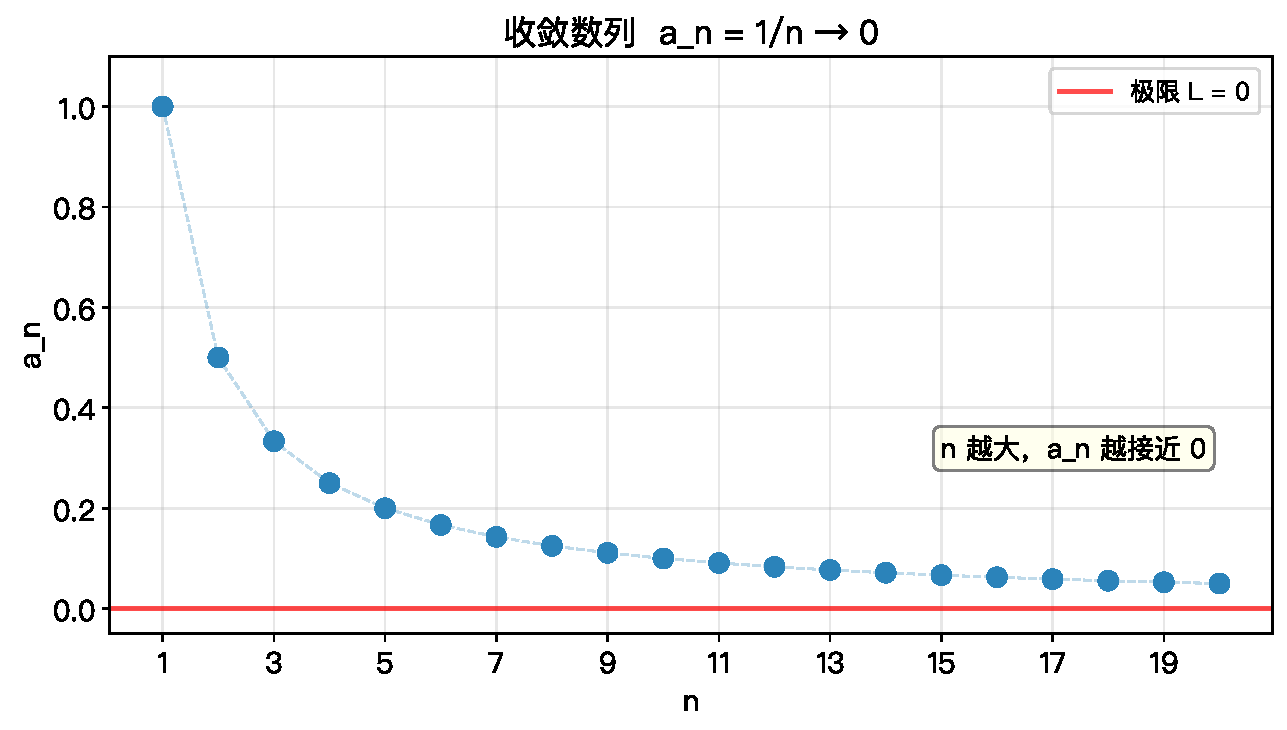
\includegraphics[width=0.85\textwidth]{figures/ch10_convergent.pdf}
\end{center}

数列 \(a_n = \dfrac{1}{n}\)：
\begin{itemize}
  \item 从 1 开始，逐渐下降
  \item 越来越接近 0，但永远不等于 0
  \item \(\displaystyle \lim_{n \to \infty} \frac{1}{n} = 0\)
\end{itemize}
\end{examplebox}

\begin{examplebox}[3——更多收敛数列]
\[
(1)\; a_n = \frac{n}{n+1}：\quad a_1=\frac12,\; a_2=\frac23,\; a_3=\frac34,\; \ldots \to 1
\]
\[
(2)\; a_n = \frac{1}{2^n}：\quad a_1=\frac12,\; a_2=\frac14,\; a_3=\frac18,\; \ldots \to 0
\]
\[
(3)\; a_n = \frac{1}{n^2}：\quad a_1=1,\; a_2=\frac14,\; a_3=\frac19,\; \ldots \to 0
\]

\textbf{验证 \(\lim_{n \to \infty} \dfrac{n}{n+1} = 1\)：}
\[
n=10: \frac{10}{11} \approx 0.909,\quad
n=100: \frac{100}{101} \approx 0.990,\quad
n=1000: \frac{1000}{1001} \approx 0.999
\]
确实越来越接近 1。
\end{examplebox}


% ============================================================
\section{发散数列——没有极限}
% ============================================================

不是所有数列都有极限。有三种常见的发散情况。

\subsection{趋于无穷}

\begin{examplebox}[4——发散到无穷大]
\begin{center}
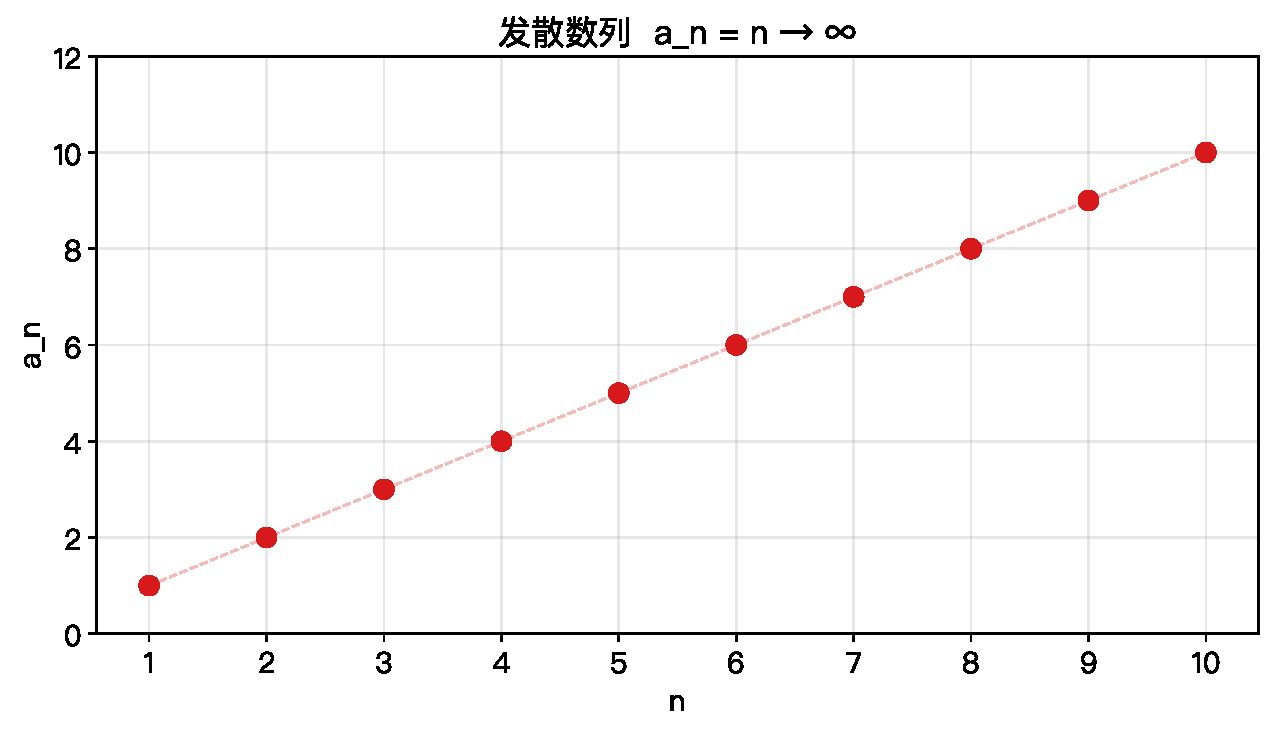
\includegraphics[width=0.85\textwidth]{figures/ch10_divergent.pdf}
\end{center}

数列 \(a_n = n\)：\(1, 2, 3, 4, \ldots\)——越来越大，没有上限。

这时我们说"极限不存在"或"发散到无穷大"。

有时也记作 \(\displaystyle \lim_{n \to \infty} n = \infty\)，但这只是一种记号，\textbf{不是真正的极限}（因为无穷大不是一个数）。
\end{examplebox}

\subsection{振荡发散}

\begin{examplebox}[5——振荡发散]
\begin{center}
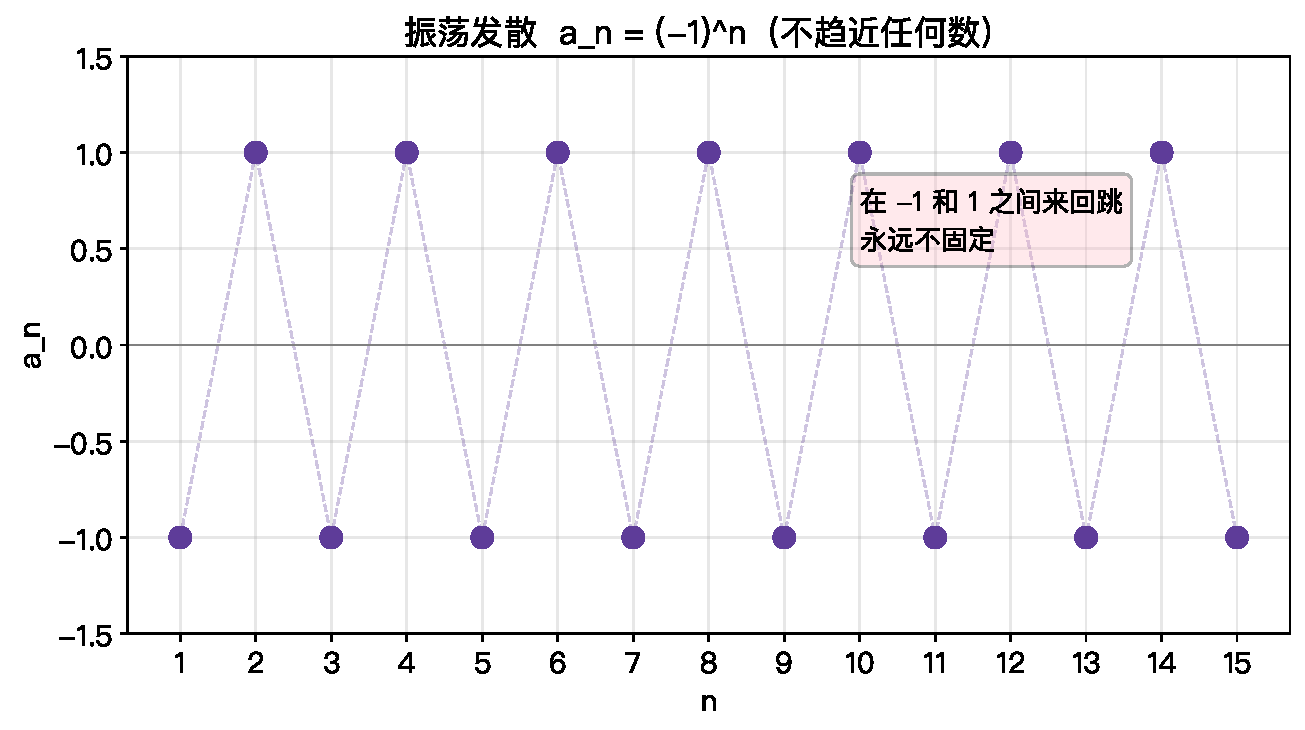
\includegraphics[width=0.85\textwidth]{figures/ch10_oscillating_divergent.pdf}
\end{center}

数列 \(a_n = (-1)^n\)：\(-1, 1, -1, 1, -1, 1, \ldots\)

它既不趋近任何数，也不趋于无穷——它在两个值之间来回跳。\\
这种发散叫\textbf{振荡发散}。
\end{examplebox}


% ============================================================
\section{极限的"ε带"几何意义}
% ============================================================

收敛数列的核心特征是：\textbf{从某项之后，所有项都"挤"在极限附近的一个小范围内}。

\begin{examplebox}[6——ε带的直观理解]
\begin{center}
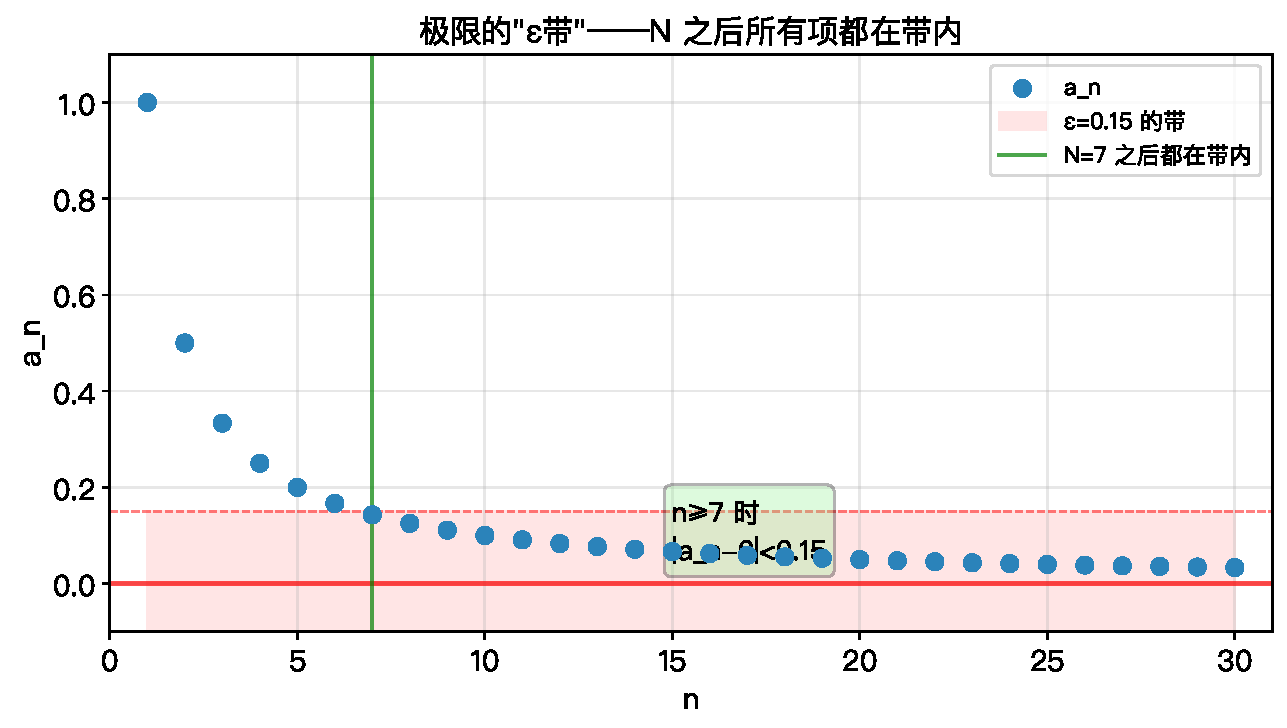
\includegraphics[width=0.85\textwidth]{figures/ch10_epsilon_band.pdf}
\end{center}

取一个很小的正数 \(\varepsilon\)（读作"伊普西龙"），在极限 \(L=0\) 周围画一条宽为 \(2\varepsilon\) 的带：
\begin{itemize}
  \item 红色带：\(|a_n - 0| < \varepsilon\) 的范围
  \item 从 \(n \ge 7\) 开始，所有项都落在这个带内
  \item \(n\) 越大，带可以取得越窄，但总存在一个 \(N\) 让之后的项都在带内
\end{itemize}

这就是\textbf{极限的核心思想}：不管你把带子取得多窄（多小的 \(\varepsilon\)），
总能找到一项 \(N\)，使得 \(N\) 之后的所有项都在带子里。
\end{examplebox}


% ============================================================
\section{常见极限的直观判断}
% ============================================================

\begin{examplebox}[7——几个重要极限]
\[
(1)\; \lim_{n \to \infty} \frac{1}{n^p} = 0 \quad (p > 0)
\]
\[
(2)\; \lim_{n \to \infty} q^n = 0 \quad (|q| < 1)
\]
\[
(3)\; \lim_{n \to \infty} \sqrt[n]{a} = 1 \quad (a > 0)
\]

\textbf{验证：}
\[
\frac{1}{\sqrt{n}} \to 0：\; \frac{1}{\sqrt{100}} = 0.1,\; \frac{1}{\sqrt{10000}} = 0.01
\]
\[
\left(\frac{1}{2}\right)^n \to 0：\; \left(\frac{1}{2}\right)^{10} = \frac{1}{1024} \approx 0.001
\]
\[
\sqrt[n]{2} \to 1：\; \sqrt[10]{2} \approx 1.072,\; \sqrt[100]{2} \approx 1.007
\]
\end{examplebox}


% ============================================================
\section{符号卡片}
% ============================================================

\begin{symbolcard}
\(\displaystyle \lim_{n \to \infty}\) & \verb|\lim_{n\to\infty}| & 读作"当 n 趋向无穷时的极限" & 极限符号 \\
\(\varepsilon\) & \verb|\varepsilon| & 读作"伊普西龙" & 任意小的正数 \\
\(a_n \to L\) & \verb|a_n \to L| & 读作"a n 趋近于 L" & 数列收敛到 L \\
发散 & —— & 读作"fā sàn" & 没有极限 \\
\end{symbolcard}


% ============================================================
\section{本章小结}
% ============================================================

\begin{progressbox}
\textbf{极限的直观}：\(n\) 越大，\(a_n\) 越接近 \(L\)

\textbf{收敛}：有极限（如 \(\dfrac{1}{n} \to 0\)，\(\dfrac{n}{n+1} \to 1\)）

\textbf{发散}：没有极限——可能趋于无穷，可能振荡

\textbf{ε带思想}：对任意 \(\varepsilon > 0\)，存在 \(N\) 使 \(n \ge N\) 时 \(|a_n - L| < \varepsilon\)

\textbf{重要极限}：\(\dfrac{1}{n^p} \to 0\)（\(p>0\)），\(q^n \to 0\)（\(|q|<1\)），\(\sqrt[n]{a} \to 1\)（\(a>0\)）
\end{progressbox}

\subsection*{通往下一章}

\textbf{这一章}你从直观上理解了"极限"是什么——数列趋近于一个数。

\textbf{下一章}将是数学分析中\textbf{第一次真正严格的定义}：
用 ε-N 语言精确地定义极限。准备好了吗？


% ============================================================
% 习题
% ============================================================
\section{习题}

% ===== 送分 =====

\begin{exercise}[0]
写出 \(\displaystyle\lim_{n\to\infty} \frac{1}{n}\) 的值。
\end{exercise}

\begin{exercise}[0]
判断：数列 \(a_n = n\) 是收敛还是发散？
\end{exercise}

\begin{exercise}[0]
判断：数列 \(a_n = (-1)^n\) 是收敛还是发散？
\end{exercise}

\begin{exercise}[0]
如果 \(\displaystyle\lim_{n\to\infty} a_n = 5\)，当 \(n\) 很大时，\(a_n\) 接近多少？
\end{exercise}

% ===== 简单 =====

\begin{exercise}[1]
计算 \(a_n = \dfrac{n}{n+1}\) 在 \(n=1, 10, 100, 1000\) 时的值，并猜测极限。
\end{exercise}

\begin{exercise}[1]
判断以下数列是否收敛（若收敛，极限是多少）：
\[
(1)\; a_n = \frac{1}{n^2} \qquad
(2)\; a_n = 3 + \frac{1}{n} \qquad
(3)\; a_n = (-1)^n n
\]
\end{exercise}

\begin{exercise}[1]
已知 \(\displaystyle\lim_{n\to\infty} a_n = 2\)，当 \(n\) 很大时，\(1 + a_n\) 接近多少？
\end{exercise}

\begin{exercise}[1]
填空：若 \(|q| < 1\)，则 \(\displaystyle\lim_{n\to\infty} q^n = \_\_\_\_\)。
\end{exercise}

% ===== 基础 =====

\begin{exercise}[2]
求极限（利用已知结论）：
\[
(1)\; \lim_{n\to\infty} \frac{1}{\sqrt{n}} \qquad
(2)\; \lim_{n\to\infty} \left(\frac{2}{3}\right)^n \qquad
(3)\; \lim_{n\to\infty} \frac{n}{2n+1}
\]
\end{exercise}

\begin{exercise}[2]
写出一个收敛到 3 的数列（至少写出通项公式）。
\end{exercise}

\begin{exercise}[2]
举例说明：一个数列可以有界但不收敛。
\end{exercise}

\begin{exercise}[2]
已知 \(a_n = \dfrac{2n+1}{n}\)，求 \(\displaystyle\lim_{n\to\infty} a_n\)。
\end{exercise}

% ===== 普通 =====

\begin{exercise}[3]
求极限：
\[
(1)\; \lim_{n\to\infty} \frac{3n^2 + 2}{n^2 + 1} \qquad
(2)\; \lim_{n\to\infty} \frac{n + 1}{n^2 + 2}
\]
（提示：分子分母同除以最高次项）
\end{exercise}

\begin{exercise}[3]
已知 \(a_n = \dfrac{1}{2^n}\)，求满足 \(|a_n - 0| < 0.001\) 的最小 \(n\)。
\end{exercise}

\begin{exercise}[3]
证明：数列 \(a_n = \dfrac{1}{n}\) 是递减且有下界的。
\end{exercise}

\begin{exercise}[3]
观察数列 \(a_n = \sqrt{n+1} - \sqrt{n}\) 的前几项，猜猜极限是多少？
（提示：有理化 \( \sqrt{n+1} - \sqrt{n} = \dfrac{1}{\sqrt{n+1} + \sqrt{n}} \)）
\end{exercise}

\begin{exercise}[3]
数列 \(a_n = 0.333\ldots 3\)（\(n\) 个 3）的极限是多少？
\end{exercise}

% ===== 中等 =====

\begin{exercise}[4]
用极限的 ε 带思想解释：为什么 \(\displaystyle\lim_{n\to\infty} \frac{1}{n^2} = 0\)？
取 \(\varepsilon = 0.01\)，找到对应的 \(N\)。
\end{exercise}

\begin{exercise}[4]
若 \(\displaystyle\lim_{n\to\infty} a_n = 3\)，证明 \(\displaystyle\lim_{n\to\infty} (2a_n - 1) = 5\)。
\end{exercise}

\begin{exercise}[4]
求极限：
\[
\lim_{n\to\infty} \left(\frac{1}{n} + \frac{2}{n} + \frac{3}{n} + \cdots + \frac{n}{n}\right) \frac{1}{n}
\]
（提示：先求和，再取极限）
\end{exercise}

\begin{exercise}[4]
已知数列 \(a_n = \dfrac{n}{2^n}\)，计算前几项，猜测极限。
（提示：\(2^n\) 的增长比 \(n\) 快得多）
\end{exercise}

\begin{exercise}[4]
判断：若 \(a_n\) 收敛，则 \(a_n\) 一定有界。这个说法对吗？为什么？
\end{exercise}

% ===== 进阶 =====

\begin{exercise}[5]
已知 \(a_n = \dfrac{n^2 + n + 1}{3n^2 - 2n + 4}\)，求 \(\displaystyle\lim_{n\to\infty} a_n\)。
\end{exercise}

\begin{exercise}[5]
构造一个数列，它不收敛、不趋于无穷、也不是振荡发散（提示：考虑 \(a_n = \sin n\)）。
\end{exercise}

\begin{exercise}[5]
若 \(a_n \to 0\)，\(b_n\) 有界，证明 \(a_n b_n \to 0\)。
\end{exercise}

\begin{exercise}[5]
证明：若 \(\displaystyle\lim_{n\to\infty} a_n = L\)，则 \(\displaystyle\lim_{n\to\infty} |a_n| = |L|\)。
（提示：利用 \(||a_n| - |L|| \le |a_n - L|\)）
\end{exercise}

% ===== 拔高 =====

\begin{exercise}[6]
数列 \(a_n = \left(1 + \dfrac{1}{n}\right)^n\) 是单调递增且有上界的。
\begin{enumerate}
  \item[(1)] 计算 \(a_1, a_2, a_5, a_{10}, a_{100}\)（用计算器或代码）
  \item[(2)] 这个数列的极限是一个著名的常数——是多少？
\end{enumerate}
\end{exercise}

\begin{exercise}[6]
设 \(a_n = \dfrac{1 \times 3 \times 5 \times \cdots \times (2n-1)}{2 \times 4 \times 6 \times \cdots \times (2n)}\)。
\begin{enumerate}
  \item[(1)] 计算 \(a_1, a_2, a_3, a_4\)
  \item[(2)] 证明 \(a_n\) 递减且有下界
  \item[(3)] 猜猜极限是多少？
\end{enumerate}
\end{exercise}

\begin{exercise}[6]
已知 \(a_1 = 1\)，\(a_{n+1} = \dfrac{1}{2}\left(a_n + \dfrac{2}{a_n}\right)\)。
\begin{enumerate}
  \item[(1)] 计算 \(a_2, a_3, a_4, a_5\)（保留小数）
  \item[(2)] 猜猜极限——它逼近什么数？
\end{enumerate}
\end{exercise}

% ===== 极难 =====

\begin{exercise}[7]
设 \(a_1 = 1\)，\(a_{n+1} = \dfrac{a_n + 2}{a_n + 1}\)。
\begin{enumerate}
  \item[(1)] 证明 \(1 \le a_n \le 2\) 对所有 \(n\) 成立
  \item[(2)] 证明 \(\{a_n\}\) 是单调的（递增还是递减？）
  \item[(3)] 求 \(\displaystyle\lim_{n\to\infty} a_n\)（提示：设极限为 \(L\)，在递推式两边取极限）
\end{enumerate}

\textbf{说明：} 这道题展示了求极限的重要方法——
先证单调有界（保证极限存在），再在递推式中取极限解出 \(L\)。
这是数学分析中最经典的方法之一。
\end{exercise}

% ============================================================
% 第11章：ε-N 语言——极限的严格定义
% ============================================================

\chapter{ε-N 语言——极限的严格定义}

\begin{applicationbox}
\textbf{学完本章你能做什么？}
\begin{enumerate}
  \item 用 \textbf{ε-N 语言} 精确地定义"极限"——不再依赖直觉
  \item 用 ε-N 证明简单的极限（如 \(\dfrac{1}{n} \to 0\)）
  \item 掌握收敛数列的性质：唯一性、有界性、保号性
  \item 学会极限的四则运算法则
\end{enumerate}
\end{applicationbox}


% ============================================================
\section{从第10章来——从"趋近"到"精确"}
% ============================================================

第10章我们说"\(\lim a_n = L\) 意思是 \(a_n\) 越来越接近 \(L\)"。

但什么叫"越来越接近"？多近才算"足够近"？

数学家的回答是：

\begin{quote}
\textbf{不管你要多近（多小的 \(\varepsilon\)），我都能找到一项 \(N\)，使得 \(N\) 之后的所有项都在这个范围内。}
\end{quote}

这就是 ε-N 语言的核心思想。它把"无限趋近"这个模糊的概念，变成了\textbf{一个关于 \(\varepsilon\) 和 \(N\) 的精确陈述}。


% ============================================================
\section{ε-N 定义}
% ============================================================

\begin{definitionbox}[数列极限的 ε-N 定义]
设 \(\{a_n\}\) 是一个数列，\(L\) 是一个实数。

如果对\textbf{任意}给定的 \(\varepsilon > 0\)，都\textbf{存在}一个正整数 \(N\)，
使得当 \(n > N\) 时，有
\[
|a_n - L| < \varepsilon
\]
则称 \(\{a_n\}\) \textbf{收敛}于 \(L\)，记作 \(\displaystyle \lim_{n \to \infty} a_n = L\)。

如果不存在这样的 \(L\)，则称 \(\{a_n\}\) \textbf{发散}。
\end{definitionbox}

\begin{examplebox}[1——把定义"翻译"成中文]
\[
\lim_{n \to \infty} \frac{1}{n} = 0
\]

ε-N 语言翻译：

\begin{center}
\fcolorbox{green!30}{green!5}{\parbox{0.85\textwidth}{
\textbf{任给你一个正数 \(\varepsilon\)（不管多小），}\\
\textbf{我都能找到一个 \(N\)，使得从第 \(N+1\) 项开始，}\\
\textbf{所有 \(\dfrac{1}{n}\) 与 0 的差都小于 \(\varepsilon\)。}
}}
\end{center}

\textbf{举个例子：}
\begin{itemize}
  \item 取 \(\varepsilon = 0.1\)：要求 \(|\frac{1}{n} - 0| < 0.1\)，即 \(\frac{1}{n} < 0.1\)，\(n > 10\)。取 \(N = 10\)。
  \item 取 \(\varepsilon = 0.01\)：要求 \(\frac{1}{n} < 0.01\)，\(n > 100\)。取 \(N = 100\)。
  \item 取 \(\varepsilon = 0.001\)：要求 \(\frac{1}{n} < 0.001\)，\(n > 1000\)。取 \(N = 1000\)。
\end{itemize}

\(\varepsilon\) 越小，需要的 \(N\) 越大——但\textbf{总能找到}。
\end{examplebox}


% ============================================================
\section{用 ε-N 证明极限}
% ============================================================

\begin{examplebox}[2——证明 1/n 趋于 0]
\textbf{证明：}

对任意 \(\varepsilon > 0\)，我们要找 \(N\) 使得 \(n > N\) 时 \(|\frac{1}{n} - 0| < \varepsilon\)。

\[
\left|\frac{1}{n} - 0\right| = \frac{1}{n} < \varepsilon \;\Longleftrightarrow\; n > \frac{1}{\varepsilon}
\]

所以取 \(N = \left\lceil \frac{1}{\varepsilon} \right\rceil\)（\(\lceil\cdot\rceil\) 是向上取整），
则当 \(n > N\) 时，\(n > \frac{1}{\varepsilon}\)，从而 \(\frac{1}{n} < \varepsilon\)。

所以 \(\displaystyle \lim_{n\to\infty} \frac{1}{n} = 0\quad\blacksquare\)

\textbf{验证：} 若 \(\varepsilon = 0.01\)，则 \(N = \lceil 1/0.01 \rceil = 100\)。\\
当 \(n = 101\) 时，\(1/101 \approx 0.0099 < 0.01\) [OK]
\end{examplebox}

\begin{examplebox}[3——证明 n/(2n+1) 趋于 1/2]
\textbf{分析：}
\[
\left|\frac{n}{2n+1} - \frac{1}{2}\right|
= \left|\frac{2n - (2n+1)}{2(2n+1)}\right|
= \left|\frac{-1}{2(2n+1)}\right|
= \frac{1}{2(2n+1)} < \frac{1}{4n}
\]

\textbf{证明：} 对任意 \(\varepsilon > 0\)，要 \(\frac{1}{2(2n+1)} < \varepsilon\)。

由 \(\frac{1}{2(2n+1)} < \frac{1}{4n}\)，只需 \(\frac{1}{4n} < \varepsilon\)，即 \(n > \frac{1}{4\varepsilon}\)。

取 \(N = \left\lceil \frac{1}{4\varepsilon} \right\rceil\)，则当 \(n > N\) 时：
\[
\left|\frac{n}{2n+1} - \frac{1}{2}\right| = \frac{1}{2(2n+1)} < \frac{1}{4n} < \varepsilon
\]

所以 \(\displaystyle \lim_{n\to\infty} \frac{n}{2n+1} = \frac{1}{2}\quad\blacksquare\)
\end{examplebox}

\begin{examplebox}[4——证明 1/2的n次方 趋于 0]
\textbf{分析：} 要 \(\frac{1}{2^n} < \varepsilon\)，即 \(2^n > \frac{1}{\varepsilon}\)。

两边取对数：\(n \ln 2 > \ln\frac{1}{\varepsilon}\)，即 \(n > \frac{\ln(1/\varepsilon)}{\ln 2}\)。

\textbf{证明：} 对任意 \(\varepsilon > 0\)，取 \(N = \left\lceil \frac{\ln(1/\varepsilon)}{\ln 2} \right\rceil\)，
则当 \(n > N\) 时，\(2^n > 2^N \ge \frac{1}{\varepsilon}\)，从而 \(\frac{1}{2^n} < \varepsilon\)。

所以 \(\displaystyle \lim_{n\to\infty} \frac{1}{2^n} = 0\quad\blacksquare\)

\textbf{验证：} 取 \(\varepsilon = 0.001\)，则 \(N = \lceil \ln(1000)/\ln 2 \rceil = \lceil 6.91/0.693 \rceil = \lceil 9.97 \rceil = 10\)。\\
当 \(n=10\) 时，\(1/2^{10} = 1/1024 \approx 0.00098 < 0.001\) [OK]
\end{examplebox}


% ============================================================
\section{ε-N 的几何意义}
% ============================================================

\begin{examplebox}[5——ε 越小，N 越大]
\begin{center}
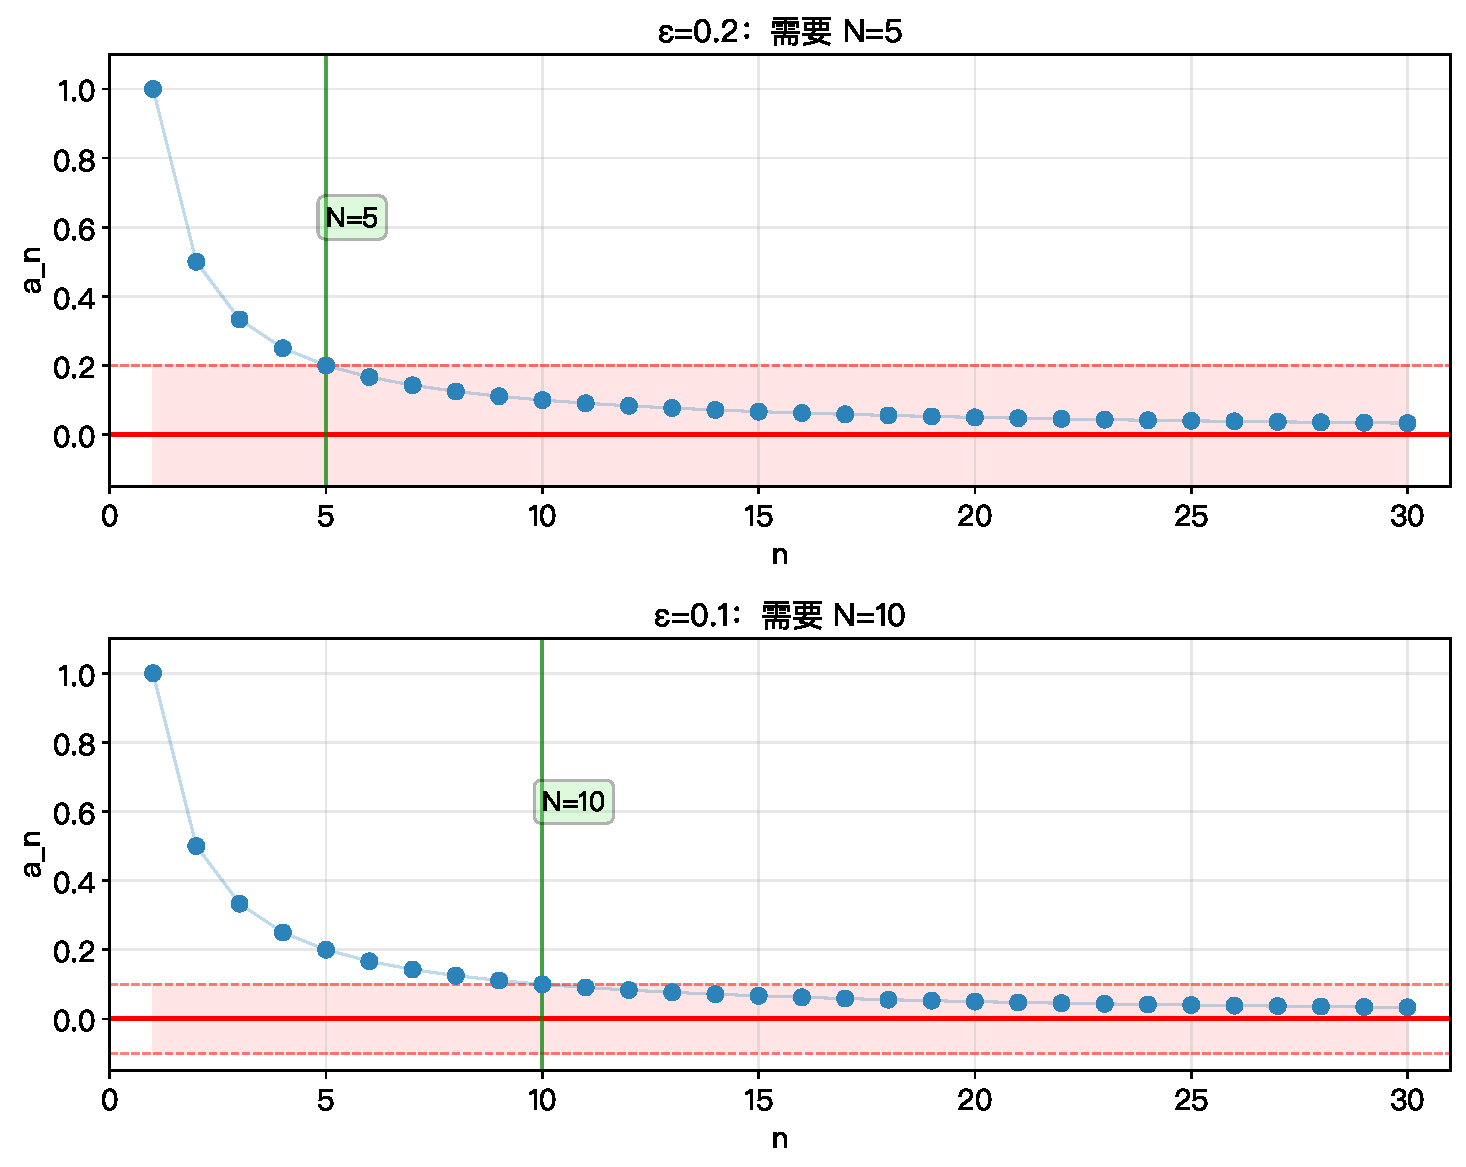
\includegraphics[width=0.85\textwidth]{figures/ch11_epsilon_N_demo.pdf}
\end{center}

\textbf{上图：} \(\varepsilon = 0.2\)，需要 \(N = 5\)（从第 6 项开始都在带内）\\
\textbf{下图：} \(\varepsilon = 0.1\)，需要 \(N = 10\)（从第 11 项开始都在带内）

\(\varepsilon\) 越小——要求越精确——需要等待的项数 \(N\) 就越大。
但\textbf{不管多小的 \(\varepsilon\)，总存在有限的 \(N\)}——这就是极限的本质。
\end{examplebox}


% ============================================================
\section{收敛数列的基本性质}
% ============================================================

\begin{theorembox}[极限的唯一性]
如果 \(\displaystyle\lim_{n\to\infty} a_n = L\) 且 \(\displaystyle\lim_{n\to\infty} a_n = M\)，则 \(L = M\)。

\textbf{解释：} 一个数列不能收敛到两个不同的数。极限如果存在，必定唯一。
\end{theorembox}

\begin{theorembox}[收敛数列必有界]
如果 \(\displaystyle\lim_{n\to\infty} a_n = L\)，则存在 \(M > 0\) 使得 \(|a_n| \le M\) 对所有 \(n\) 成立。

\textbf{解释：} 收敛的数列一定是有界的（但不一定单调）。
反过来不对——有界不一定收敛（如 \((-1)^n\) 有界但不收敛）。
\end{theorembox}

\begin{theorembox}[极限的保号性]
如果 \(\displaystyle\lim_{n\to\infty} a_n = L > 0\)，则存在 \(N\) 使得 \(n > N\) 时 \(a_n > 0\)。

\textbf{解释：} 如果极限是正数，那么足够靠后的项也都是正数。
\end{theorembox}


% ============================================================
\section{极限的四则运算}
% ============================================================

\begin{theorembox}[极限的四则运算法则]
如果 \(\displaystyle\lim_{n\to\infty} a_n = A\)，\(\displaystyle\lim_{n\to\infty} b_n = B\)，则：
\begin{align*}
  \lim_{n\to\infty} (a_n \pm b_n) &= A \pm B \\
  \lim_{n\to\infty} (a_n \cdot b_n) &= A \cdot B \\
  \lim_{n\to\infty} \frac{a_n}{b_n} &= \frac{A}{B} \quad (B \neq 0)
\end{align*}
\end{theorembox}

\begin{examplebox}[6——用四则运算法则求极限]
\[
\lim_{n\to\infty} \frac{3n^2 + 2n - 1}{2n^2 + 5}
\]

分子分母同除以 \(n^2\)：
\[
\frac{3n^2 + 2n - 1}{2n^2 + 5} = \frac{3 + \frac{2}{n} - \frac{1}{n^2}}{2 + \frac{5}{n^2}}
\]

因为 \(\frac{1}{n} \to 0\)，\(\frac{1}{n^2} \to 0\)，所以：
\[
\lim_{n\to\infty} \frac{3n^2 + 2n - 1}{2n^2 + 5} = \frac{3 + 0 - 0}{2 + 0} = \frac{3}{2}
\]

\textbf{口诀：} 分子分母同除以最高次项，低次项在 \(n\to\infty\) 时趋于 0。
\end{examplebox}


% ============================================================
\section{符号卡片}
% ============================================================

\begin{symbolcard}
\(\varepsilon\) & \verb|\varepsilon| & 读作"伊普西龙" & 任意小的正数 \\
\(N\) & —— & 读作"N" & 正整数，保证 \(n>N\) 时成立 \\
\(\lceil x \rceil\) & \verb|\lceil x\rceil| & 读作"x 的上取整" & 不小于 \(x\) 的最小整数 \\
\(|a_n-L|<\varepsilon\) & —— & 读作"epsilon" & 与极限的距离小于 epsilon \\
\end{symbolcard}


% ============================================================
\section{本章小结}
% ============================================================

\begin{progressbox}
\textbf{ε-N 定义}：\(\forall \varepsilon > 0, \exists N, n > N \Rightarrow |a_n - L| < \varepsilon\)

\textbf{证明步骤}：
\begin{enumerate}
  \item 从 \(|a_n - L|\) 出发，用不等式放大到关于 \(n\) 的简单形式
  \item 令其 \(< \varepsilon\)，解出 \(n\) 需要满足的条件
  \item 取 \(N\) 为这个条件的上取整
\end{enumerate}

\textbf{收敛数列性质}：极限唯一、收敛必有界、保号性

极限的四则运算法则：和的极限 = 极限的和，积的极限 = 极限的积，商的极限 = 极限的商
\end{progressbox}

\subsection*{通往下一章}

\textbf{这一章}你掌握了极限的严格定义和基本性质。

\textbf{下一章}我们学习判断极限存在的两大工具——
\textbf{单调有界原理}和\textbf{夹逼定理}（迫敛性）。
你会看到如何在不直接求极限的情况下，判断极限是否存在并求出它的值。


% ============================================================
% 习题
% ============================================================
\section{习题}

% ===== 送分 =====

\begin{exercise}[0]
用 ε-N 语言写出 "\(\lim a_n = 3\)" 的定义。
\end{exercise}

\begin{exercise}[0]
如果对 \(\varepsilon = 0.1\) 找到 \(N = 50\)，那么 \(n = 100\) 时 \(|a_n - L|\) 一定小于 0.1 吗？
\end{exercise}

\begin{exercise}[0]
数列极限存在，则极限必\_\_\_\_（唯一/不唯一）。
\end{exercise}

\begin{exercise}[0]
若 \(a_n \to 2\)，则 \(2a_n \to\) \_\_\_\_。
\end{exercise}

% ===== 简单 =====

\begin{exercise}[1]
用 ε-N 语言证明 \(\displaystyle \lim_{n\to\infty} \frac{1}{n^2} = 0\)。
\end{exercise}

\begin{exercise}[1]
若 \(\varepsilon = 0.01\)，对于 \(\frac{1}{n} \to 0\)，对应的 \(N\) 至少是多少？
\end{exercise}

\begin{exercise}[1]
判断对错：若数列有界，则一定收敛。
\end{exercise}

\begin{exercise}[1]
求极限：
\[
\lim_{n\to\infty} \frac{n+2}{n+1}
\]
\end{exercise}

% ===== 基础 =====

\begin{exercise}[2]
用 ε-N 语言证明 \(\displaystyle \lim_{n\to\infty} \frac{1}{\sqrt{n}} = 0\)。
\end{exercise}

\begin{exercise}[2]
已知 \(a_n \to 3\)，用四则运算法则求：
\[
\lim_{n\to\infty} (2a_n + 1),\quad \lim_{n\to\infty} \frac{a_n}{a_n + 1}
\]
\end{exercise}

\begin{exercise}[2]
若 \(\displaystyle \lim_{n\to\infty} a_n = L\)，证明 \(\displaystyle \lim_{n\to\infty} (a_n)^2 = L^2\)。
（提示：\(|a_n^2 - L^2| = |a_n - L| \cdot |a_n + L|\)，再说明 \(|a_n + L|\) 有界）
\end{exercise}

\begin{exercise}[2]
求极限：
\[
\lim_{n\to\infty} \frac{2n^2 - 3n + 1}{5n^2 + 4n - 2}
\]
\end{exercise}

% ===== 普通 =====

\begin{exercise}[3]
用 ε-N 语言证明 \(\displaystyle \lim_{n\to\infty} \frac{2n}{n+3} = 2\)。
\end{exercise}

\begin{exercise}[3]
求极限：
\[
\lim_{n\to\infty} \frac{n^3 + 2n}{2n^3 - n^2 + 1}
\]
\end{exercise}

\begin{exercise}[3]
已知 \(a_n \to A\)，\(b_n \to B\)，证明 \(a_n b_n \to AB\)。
\end{exercise}

\begin{exercise}[3]
若 \(a_n \to 0\)，\(b_n\) 有界，证明 \(a_n b_n \to 0\)。
\end{exercise}

\begin{exercise}[3]
用 ε-N 语言证明：若 \(a_n \to L\)，则 \(|a_n| \to |L|\)。
\end{exercise}

% ===== 中等 =====

\begin{exercise}[4]
求极限：
\[
\lim_{n\to\infty} (\sqrt{n+1} - \sqrt{n})
\]
（提示：有理化 \(\sqrt{n+1} - \sqrt{n} = \frac{1}{\sqrt{n+1} + \sqrt{n}}\)）
\end{exercise}

\begin{exercise}[4]
用 ε-N 语言证明 \(\displaystyle \lim_{n\to\infty} \frac{n^2}{n^2 + 1} = 1\)。
\end{exercise}

\begin{exercise}[4]
已知 \(a_1 = 1\)，\(a_{n+1} = \frac{a_n + 2}{2}\)。
\begin{enumerate}
  \item[(1)] 写出前 5 项，观察规律
  \item[(2)] 求极限（设极限为 \(L\)，在递推式两边取极限）
\end{enumerate}
\end{exercise}

\begin{exercise}[4]
求极限：
\[
\lim_{n\to\infty} \frac{1 + 2 + 3 + \cdots + n}{n^2}
\]
\end{exercise}

\begin{exercise}[4]
证明：收敛数列必有界。
（提示：取 \(\varepsilon = 1\)，则存在 \(N\) 使 \(n>N\) 时 \(|a_n - L| < 1\)，
然后前 \(N\) 项有限，后 \(N\) 项有界）
\end{exercise}

% ===== 进阶 =====

\begin{exercise}[5]
用 ε-N 语言证明 \(\displaystyle \lim_{n\to\infty} \frac{\sin n}{n} = 0\)。
（提示：\(|\sin n| \le 1\)）
\end{exercise}

\begin{exercise}[5]
已知 \(a_n \to L\)，用 ε-N 语言证明 \(a_{n+1} \to L\)。
\end{exercise}

\begin{exercise}[5]
求极限：
\[
\lim_{n\to\infty} \frac{n^2 + (-1)^n n}{n^2 + 1}
\]
\end{exercise}

\begin{exercise}[5]
已知 \(a_1 = \sqrt{2}\)，\(a_{n+1} = \sqrt{2 + a_n}\)。
\begin{enumerate}
  \item[(1)] 写出前 3 项
  \item[(2)] 若极限存在，求它的值
\end{enumerate}
\end{exercise}

% ===== 拔高 =====

\begin{exercise}[6]
设 \(a_n = \frac{n^k}{2^n}\)（\(k\) 是正整数）。
试说明为什么 \(\displaystyle \lim_{n\to\infty} a_n = 0\)。
（提示：指数 \(2^n\) 的增长最终会超过任何幂函数 \(n^k\)）
\end{exercise}

\begin{exercise}[6]
用 ε-N 语言证明 \(\displaystyle \lim_{n\to\infty} \frac{2^n}{n!} = 0\)。
（提示：\(n \ge 4\) 时 \(\frac{2^n}{n!} \le \frac{2}{n}\)）
\end{exercise}

\begin{exercise}[6]
已知 \(a_n \to L\)，定义 \(b_n = \frac{a_1 + a_2 + \cdots + a_n}{n}\)（算术平均）。
证明 \(b_n \to L\)。
（提示：把前 \(N\) 项和后 \(n-N\) 项分开处理）
\end{exercise}

% ===== 极难 =====

\begin{exercise}[7]
设 \(a_1 = 1\)，\(a_{n+1} = \frac{1}{2}\left(a_n + \frac{2}{a_n}\right)\)。
\begin{enumerate}
  \item[(1)] 证明 \(a_n^2 > 2\)（\(n \ge 2\)）
  \item[(2)] 证明 \(a_n\) 单调递减
  \item[(3)] 求 \(\displaystyle \lim_{n\to\infty} a_n\)
\end{enumerate}

\textbf{说明：} 这是牛顿法求 \(\sqrt{2}\) 的迭代序列。
先证有下界（\(a_n > \sqrt{2}\)），再证递减，最后两边取极限解出 \(L = \sqrt{2}\)。
这是数学分析中最经典的极限问题之一。
\end{exercise}

% ============================================================
% 第12章：极限存在判别法——单调有界、夹逼、柯西
% ============================================================

\chapter{极限存在判别法——单调有界与夹逼定理}

\begin{applicationbox}
\textbf{学完本章你能做什么？}
\begin{enumerate}
  \item 用\textbf{单调有界原理}判断数列收敛——这是数学分析中最常用的方法
  \item 用\textbf{夹逼定理}（迫敛性）求极限——把复杂数列夹在两个简单数列之间
  \item 了解\textbf{柯西收敛准则}——不依赖极限值也能判断收敛
\end{enumerate}
\end{applicationbox}


% ============================================================
\section{从第11章来——如何判断极限存在？}
% ============================================================

第11章我们学了极限的 ε-N 定义——但用定义证明收敛，需要\textbf{先知道极限值}。

如果不知道极限值呢？比如数列 \(a_n = (1 + \frac{1}{n})^n\)——它有极限吗？极限是多少？

这就需要用到本章的两个强大工具：
\begin{itemize}
  \item \textbf{单调有界原理}：如果数列单调且有界，则一定收敛
  \item \textbf{夹逼定理}：如果两个数列收敛到同一个数，中间那个也收敛
\end{itemize}


% ============================================================
\section{单调有界原理}
% ============================================================

\begin{theorembox}[单调有界原理]
如果数列 \(\{a_n\}\) 是\textbf{单调递增}且\textbf{有上界}的，那么它一定收敛。

同样，如果数列是\textbf{单调递减}且\textbf{有下界}的，那么它一定收敛。
\end{theorembox}

\begin{examplebox}[1——单调有界的直观]
\begin{center}
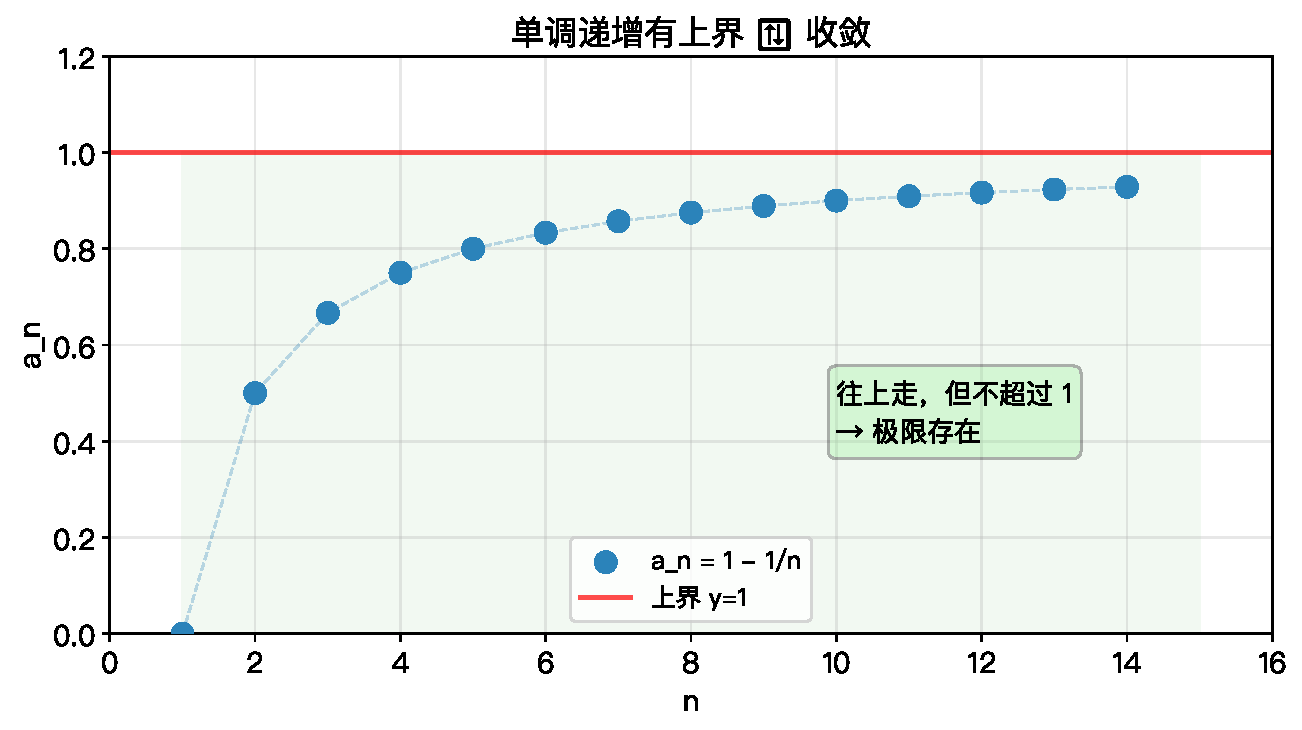
\includegraphics[width=0.85\textwidth]{figures/ch12_monotone_bounded.pdf}
\end{center}

数列 \(a_n = 1 - \frac{1}{n}\)：
\begin{itemize}
  \item \textbf{单调递增}：\(a_1=0, a_2=0.5, a_3\approx0.667, a_4=0.75, \ldots\)——一直往上走
  \item \textbf{有上界}：永远不超过 1（因为 \(\frac{1}{n} > 0\)，所以 \(1 - \frac{1}{n} < 1\)）
  \item \(\rightarrow\) \textbf{收敛}，极限为 1
\end{itemize}

\textbf{为什么单调有界一定收敛？}
从直观看：单调递增有上界，数列一直往上走但不能突破上界，所以它只能"挤"在某个数附近——这个数就是极限。
\end{examplebox}

\begin{examplebox}[2——求极限的重要方法]
用单调有界原理求极限的\textbf{标准步骤}：

\begin{enumerate}
  \item 证明数列\textbf{单调}（常用 \(a_{n+1} - a_n \ge 0\) 或 \(\frac{a_{n+1}}{a_n} \ge 1\)）
  \item 证明数列\textbf{有界}（找到上界或下界）
  \item 由单调有界原理 \(\Rightarrow\) 极限存在（设为 \(L\)）
  \item 在递推式两边取极限，解出 \(L\)
\end{enumerate}
\end{examplebox}

\begin{examplebox}[3——用单调有界求极限]
已知 \(a_1 = 2\)，\(a_{n+1} = \frac{1}{2}\left(a_n + \frac{2}{a_n}\right)\)。

\textbf{第1步：证有下界}
\[
a_{n+1} = \frac{1}{2}\left(a_n + \frac{2}{a_n}\right) \ge \frac{1}{2} \cdot 2\sqrt{a_n \cdot \frac{2}{a_n}} = \sqrt{2}
\]
（用基本不等式：\(x + \frac{2}{x} \ge 2\sqrt{2}\)）

所以 \(a_n \ge \sqrt{2}\) 对所有 \(n\) 成立。

\textbf{第2步：证单调递减}
\[
a_{n+1} - a_n = \frac{1}{2}\left(a_n + \frac{2}{a_n}\right) - a_n = \frac{1}{2}\left(\frac{2}{a_n} - a_n\right) = \frac{2 - a_n^2}{2a_n} \le 0
\]
（因为 \(a_n \ge \sqrt{2}\)，所以 \(a_n^2 \ge 2\)，分子 \(\le 0\)）

所以 \(a_{n+1} \le a_n\)，单调递减。

\textbf{第3步：极限存在}
单调递减有下界 \(\Rightarrow\) 极限存在，设 \(\lim a_n = L\)。

\textbf{第4步：求极限}
在递推式两边取极限：
\[
L = \frac{1}{2}\left(L + \frac{2}{L}\right) \;\Longrightarrow\; 2L = L + \frac{2}{L} \;\Longrightarrow\; L = \frac{2}{L} \;\Longrightarrow\; L^2 = 2
\]
所以 \(L = \sqrt{2}\)（因为 \(a_n > 0\)，舍去负值）。

\textbf{结论：} \(\displaystyle \lim_{n\to\infty} a_n = \sqrt{2}\)。
\end{examplebox}


% ============================================================
\section{夹逼定理（迫敛性）}
% ============================================================

\begin{theorembox}[夹逼定理]
如果存在 \(N\) 使得 \(n > N\) 时
\[
b_n \le a_n \le c_n
\]
且 \(\displaystyle \lim_{n\to\infty} b_n = \lim_{n\to\infty} c_n = L\)，
则 \(\displaystyle \lim_{n\to\infty} a_n = L\)。
\end{theorembox}

\textbf{直观理解：} 三个人挤在一条巷子里，两边的人都出去了，中间那个人也只能从那个口出去。

\begin{examplebox}[4——夹逼定理的几何意义]
\begin{center}
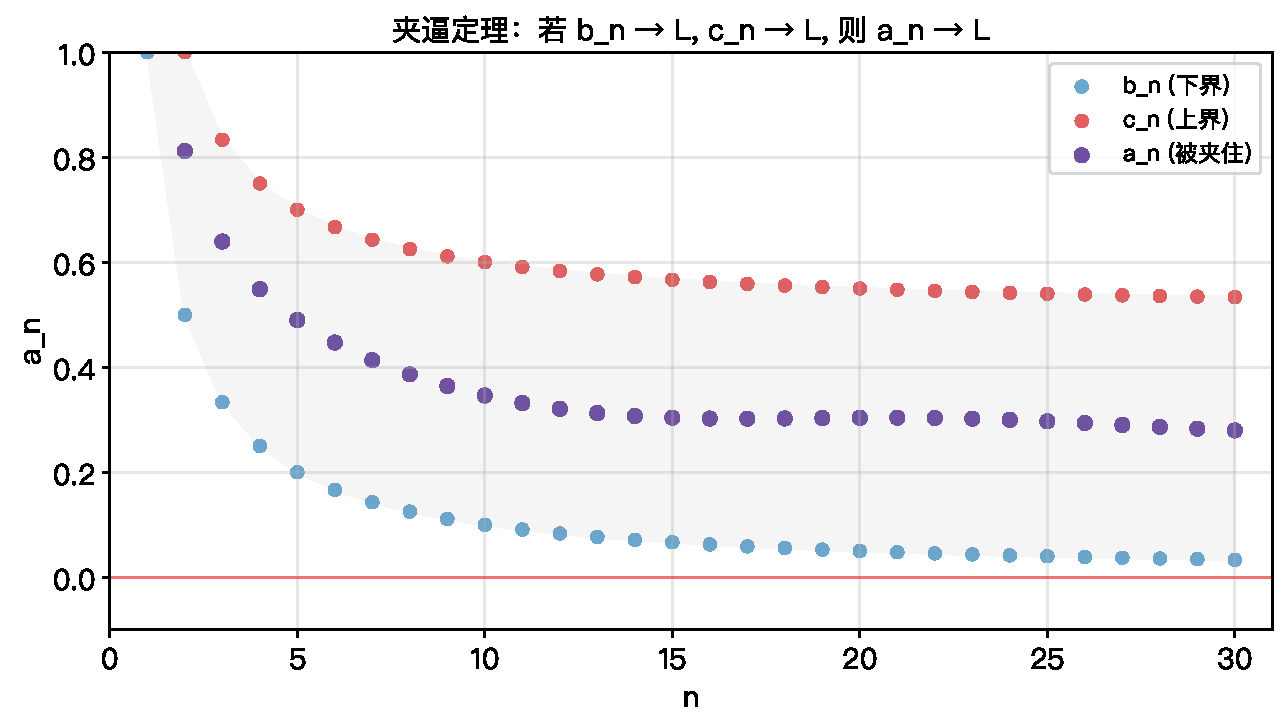
\includegraphics[width=0.85\textwidth]{figures/ch12_squeeze_theorem.pdf}
\end{center}

灰色区域是 \(b_n\) 和 \(c_n\) 夹出的范围，\(a_n\) 被限制在其中。
当 \(b_n\) 和 \(c_n\) 都趋近于同一个数时，\(a_n\) 也只能趋近于那个数。
\end{examplebox}

\begin{examplebox}[5——用夹逼定理求极限]
求 \(\displaystyle \lim_{n\to\infty} \frac{\sin n}{n}\)。

因为 \(|\sin n| \le 1\)，所以：
\[
-\frac{1}{n} \le \frac{\sin n}{n} \le \frac{1}{n}
\]

而 \(\displaystyle \lim_{n\to\infty} \left(-\frac{1}{n}\right) = 0\)，\(\displaystyle \lim_{n\to\infty} \frac{1}{n} = 0\)。

由夹逼定理：\(\displaystyle \lim_{n\to\infty} \frac{\sin n}{n} = 0\)。
\end{examplebox}

\begin{examplebox}[6——另一个例子]
求 \(\displaystyle \lim_{n\to\infty} \frac{n!}{n^n}\)。

\[
0 < \frac{n!}{n^n} = \frac{1 \cdot 2 \cdot 3 \cdots n}{n \cdot n \cdot n \cdots n} \le \frac{1}{n}
\]

而 \(0 \to 0\)，\(\frac{1}{n} \to 0\)，由夹逼定理：
\[
\lim_{n\to\infty} \frac{n!}{n^n} = 0
\]
\end{examplebox}


% ============================================================
\section{两个重要极限}
% ============================================================

\begin{theorembox}[两个重要极限]
\[
(1)\; \lim_{n\to\infty} \left(1 + \frac{1}{n}\right)^n = e
\]
\[
(2)\; \lim_{n\to\infty} \sqrt[n]{n} = 1
\]
\end{theorembox}

\begin{examplebox}[7——第一个重要极限：自然常数 \(e\)]
数列 \(a_n = \left(1 + \frac{1}{n}\right)^n\)：
\[
a_1 = 2,\; a_2 = (1.5)^2 = 2.25,\; a_3 \approx 2.37,\; a_{10} \approx 2.594
\]
\[
a_{100} \approx 2.705,\; a_{1000} \approx 2.717,\; a_{10000} \approx 2.718
\]

这个数列\textbf{单调递增且有上界}（可以证明上界为 3），
因此收敛——它的极限就是 \(e \approx 2.71828\)。

这是自然常数 \(e\) 的\textbf{定义}之一。
\end{examplebox}

\begin{examplebox}[8——第二个重要极限]
证明 \(\sqrt[n]{n} \to 1\)：

令 \(\sqrt[n]{n} = 1 + x_n\)（\(x_n > 0\)），则：
\[
n = (1 + x_n)^n \ge 1 + \frac{n(n-1)}{2}x_n^2 \quad (\text{二项式展开到第三项})
\]
\[
\Rightarrow x_n^2 \le \frac{2(n-1)}{n(n-1)} = \frac{2}{n-1}
\]
\[
\Rightarrow 0 < x_n \le \sqrt{\frac{2}{n-1}} \to 0
\]

由夹逼定理，\(x_n \to 0\)，所以 \(\sqrt[n]{n} = 1 + x_n \to 1\)。
\end{examplebox}


% ============================================================
\section{柯西收敛准则（了解）}
% ============================================================

\begin{theorembox}[柯西收敛准则]
数列 \(\{a_n\}\) 收敛的\textbf{充要条件}是：
对任意 \(\varepsilon > 0\)，存在 \(N\)，使得 \(m, n > N\) 时
\[
|a_m - a_n| < \varepsilon
\]
\end{theorembox}

\textbf{含义：} 收敛数列的项越到后面"挤得越紧"——任意两项的差最终可以任意小。

柯西准则的\textbf{优点}：不需要知道极限值就能判断收敛。\\
\textbf{缺点}：使用起来比单调有界和夹逼更复杂。


% ============================================================
\section{本章小结}
% ============================================================

\begin{progressbox}
\textbf{单调有界原理}：单调递增有上界（或递减有下界）⇒ 收敛

\textbf{证明步骤}：证单调 $\to$ 证有界 $\to$ 极限存在 $\to$ 在递推式两边取极限求值

\textbf{夹逼定理}：\(b_n \le a_n \le c_n\)，且 \(b_n, c_n \to L\) ⇒ \(a_n \to L\)

\textbf{两个重要极限}：
\[
\lim_{n\to\infty} \left(1 + \frac{1}{n}\right)^n = e,\quad
\lim_{n\to\infty} \sqrt[n]{n} = 1
\]

\textbf{柯西准则}：\(m,n\) 足够大时 \(|a_m - a_n| < \varepsilon\) ⇔ 收敛
\end{progressbox}

\subsection*{通往第二编——函数极限与连续}


% ============================================================
% 习题
% ============================================================
\section{习题}

% ===== 送分 =====

\begin{exercise}[0]
判断正误：单调递增的数列一定收敛。
\end{exercise}

\begin{exercise}[0]
判断正误：有上界的数列一定收敛。
\end{exercise}

\begin{exercise}[0]
数列 \(a_n = 1 - \frac{1}{n}\) 是否单调？是否有上界？
\end{exercise}

\begin{exercise}[0]
夹逼定理中，如果 \(b_n \le a_n \le c_n\) 且 \(b_n \to 2\)，\(c_n \to 2\)，则 \(a_n \to\) \_\_\_\_。
\end{exercise}

% ===== 简单 =====

\begin{exercise}[1]
证明数列 \(a_n = \frac{n}{n+1}\) 单调递增且有上界，并求极限。
\end{exercise}

\begin{exercise}[1]
用夹逼定理求 \(\displaystyle \lim_{n\to\infty} \frac{\cos n}{n}\)。
\end{exercise}

\begin{exercise}[1]
判断：数列 \(a_n = (-1)^n\) 是否单调？是否有界？是否收敛？
\end{exercise}

\begin{exercise}[1]
已知 \(a_n = 2 - \frac{1}{n}\)，证明它单调递增且有上界，极限是多少？
\end{exercise}

% ===== 基础 =====

\begin{exercise}[2]
用单调有界原理证明数列 \(a_n = \frac{1}{2^n}\) 收敛，并求极限。
\end{exercise}

\begin{exercise}[2]
用夹逼定理求 \(\displaystyle \lim_{n\to\infty} \frac{n + \sin n}{2n - \cos n}\)。
（提示：放大到 \(\frac{n+1}{2n-1}\)，缩小到 \(\frac{n-1}{2n+1}\)）
\end{exercise}

\begin{exercise}[2]
求极限 \(\displaystyle \lim_{n\to\infty} \left(1 + \frac{1}{n}\right)^n\)，这个极限等于什么常数？
\end{exercise}

\begin{exercise}[2]
求证：数列 \(a_n = \frac{1}{2} \cdot \frac{3}{4} \cdot \frac{5}{6} \cdots \frac{2n-1}{2n}\) 单调递减且有下界。
\end{exercise}

% ===== 普通 =====

\begin{exercise}[3]
已知 \(a_1 = 1\)，\(a_{n+1} = \sqrt{2a_n}\)。
\begin{enumerate}
  \item[(1)] 写出前 4 项
  \item[(2)] 证明 \(\{a_n\}\) 单调递增且有上界
  \item[(3)] 求极限
\end{enumerate}
\end{exercise}

\begin{exercise}[3]
用夹逼定理求 \(\displaystyle \lim_{n\to\infty} \frac{\ln n}{n}\)。
（提示：\(0 < \frac{\ln n}{n} < \frac{1}{\sqrt{n}}\) 当 \(n\) 足够大时）
\end{exercise}

\begin{exercise}[3]
已知 \(a_n = \frac{n!}{2^n}\)。证明 \(a_n \to \infty\)（发散）。
（提示：\(n \ge 4\) 时 \(\frac{a_{n+1}}{a_n} = \frac{n+1}{2} > 1\)）
\end{exercise}

\begin{exercise}[3]
求极限 \(\displaystyle \lim_{n\to\infty} \frac{2^n}{n!}\)。
（提示：\(n \ge 4\) 时 \(\frac{2^n}{n!} \le \frac{2}{n}\)，再用夹逼定理）
\end{exercise}

\begin{exercise}[3]
证明数列 \(a_n = \left(1 + \frac{1}{n}\right)^{n+1}\) 单调递减。
（提示：可以证明 \(\frac{a_{n+1}}{a_n} \le 1\)）
\end{exercise}

% ===== 中等 =====

\begin{exercise}[4]
已知 \(a_1 = \sqrt{2}\)，\(a_{n+1} = \sqrt{2 + a_n}\)。
\begin{enumerate}
  \item[(1)] 证明 \(a_n < 2\) 对所有 \(n\) 成立
  \item[(2)] 证明 \(\{a_n\}\) 单调递增
  \item[(3)] 求极限
\end{enumerate}
\end{exercise}

\begin{exercise}[4]
用夹逼定理求 \(\displaystyle \lim_{n\to\infty} \left(\frac{1}{\sqrt{n^2+1}} + \frac{1}{\sqrt{n^2+2}} + \cdots + \frac{1}{\sqrt{n^2+n}}\right)\)。
（提示：\(n\) 项，每项介于 \(\frac{1}{\sqrt{n^2+n}}\) 和 \(\frac{1}{\sqrt{n^2}}\) 之间）
\end{exercise}

\begin{exercise}[4]
已知 \(a_1 = 1\)，\(a_{n+1} = \frac{a_n}{2} + \frac{1}{a_n}\)。
\begin{enumerate}
  \item[(1)] 证明 \(a_n^2 \ge 2\)
  \item[(2)] 证明数列单调递减
  \item[(3)] 求极限
\end{enumerate}
\end{exercise}

\begin{exercise}[4]
求 \(\displaystyle \lim_{n\to\infty} \frac{1}{n^2} \left( \frac{1}{1^2} + \frac{1}{2^2} + \cdots + \frac{1}{n^2} \right)\)。
\end{exercise}

\begin{exercise}[4]
证明：若 \(0 < a < 1\)，则 \(a^n \to 0\)（用夹逼定理）。
\end{exercise}

% ===== 进阶 =====

\begin{exercise}[5]
已知 \(a_1 = 3\)，\(a_{n+1} = \frac{1}{2}\left(a_n + \frac{9}{a_n}\right)\)。
\begin{enumerate}
  \item[(1)] 证明 \(a_n \ge 3\)
  \item[(2)] 证明单调递减
  \item[(3)] 求极限
\end{enumerate}
\end{exercise}

\begin{exercise}[5]
用单调有界原理证明数列 \(a_n = \frac{1}{n+1} + \frac{1}{n+2} + \cdots + \frac{1}{2n}\) 收敛。
（提示：先证 \(a_{n+1} - a_n = \frac{1}{2n+1} - \frac{1}{2n+2} > 0\)，再证 \(a_n < 1\)）
\end{exercise}

\begin{exercise}[5]
求 \(\displaystyle \lim_{n\to\infty} \sqrt[n]{n^2 + 1}\)。
（提示：\(\sqrt[n]{n^2} \le \sqrt[n]{n^2+1} \le \sqrt[n]{2n^2}\)，且 \(\sqrt[n]{n} \to 1\)）
\end{exercise}

\begin{exercise}[5]
已知 \(0 < a_1 < 1\)，\(a_{n+1} = a_n(1 - a_n)\)。
\begin{enumerate}
  \item[(1)] 证明 \(0 < a_n < 1\) 且单调递减
  \item[(2)] 求极限
\end{enumerate}
\end{exercise}

% ===== 拔高 =====

\begin{exercise}[6]
已知 \(a_1 = 1\)，\(a_{n+1} = 1 + \frac{1}{a_n}\)。
\begin{enumerate}
  \item[(1)] 写出前 6 项，观察奇偶子列的规律
  \item[(2)] 证明 \(\{a_{2k}\}\) 和 \(\{a_{2k+1}\}\) 分别单调且收敛
  \item[(3)] 它们的极限相等吗？如果相等，求极限。
\end{enumerate}
（这个数列的极限是黄金分割比 \(\frac{1+\sqrt{5}}{2}\)——斐波那契数列的相邻项之比）
\end{exercise}

\begin{exercise}[6]
用夹逼定理证明 \(\displaystyle \lim_{n\to\infty} \frac{n}{\sqrt[n]{n!}} = e\)。
（提示：利用 \(n^n e^{-n} < n! < n^{n+1} e^{-n+1}\)，这是斯特林公式的粗略形式）
\end{exercise}

\begin{exercise}[6]
已知 \(a_1 > 0\)，\(a_{n+1} = \frac{a_n^2 + 1}{2a_n}\)。
\begin{enumerate}
  \item[(1)] 证明 \(a_n \ge 1\)
  \item[(2)] 证明单调递减
  \item[(3)] 求极限
\end{enumerate}
\end{exercise}

% ===== 极难 =====

\begin{exercise}[7]
设 \(a_1 = 1\)，\(a_{n+1} = \frac{3a_n + 2}{a_n + 2}\)。
\begin{enumerate}
  \item[(1)] 证明 \(a_n > 0\) 且有上界 2
  \item[(2)] 判断单调性并证明
  \item[(3)] 求极限
  \item[(4)] 若 \(b_n = \frac{a_n - 2}{a_n + 1}\)，证明 \(\{b_n\}\) 是等比数列
\end{enumerate}

\textbf{说明：} 这道题综合了单调有界原理和构造等比数列的技巧。
第(4)问的构造法——通过线性变换将递推式化为等比数列——是数学分析中处理递推数列的重要方法。
\end{exercise}



\textbf{第一编到此结束！} 你完成了数列极限的全部 4 章——
从数列基础到 ε-N 定义，再到单调有界和夹逼。

\textbf{第二编}我们将进入\textbf{函数极限与连续}——
把极限的思想从离散的数列扩展到连续的函数。
这是通向导数的大门。

% 第一编结束，进入第二编

% ============================================================
% 第二编：函数极限与连续
\part{函数极限与连续——从离散到连续}
% ============================================================
% 第13章：函数在无穷远处的极限——水平渐近线
% ============================================================

\chapter{函数在无穷远处的极限——水平渐近线}

\begin{applicationbox}
\textbf{学完本章你能做什么？}
\begin{enumerate}
  \item 理解函数在 \(x \to \infty\) 时的极限——数列极限的自然延伸
  \item 区分\textbf{水平渐近线}（有极限）和\textbf{无穷极限}（无界）
  \item 对比不同函数的增长速度：\(\ln x, \sqrt{x}, x, x^2, e^x\)
\end{enumerate}
\end{applicationbox}


% ============================================================
\section{从数列到函数——从离散到连续}
% ============================================================

数列极限讲的是当 \(n \to \infty\)（正整数趋向无穷）时 \(a_n\) 的行为。

函数极限讲的是当 \(x \to \infty\)（实数趋向无穷）时 \(f(x)\) 的行为。

\begin{center}
\begin{tabular}{c|c}
\textbf{数列} & \textbf{函数} \\
\hline
\(n\) 只能取正整数 & \(x\) 可取任意实数 \\
\(\displaystyle\lim_{n\to\infty} a_n = L\) & \(\displaystyle\lim_{x\to\infty} f(x) = L\) \\
离散的点 & 连续的曲线 \\
\end{tabular}
\end{center}


% ============================================================
\section{\(x \to \infty\) 时的极限}
% ============================================================

\begin{definitionbox}[函数在无穷远处的极限]
如果当 \(x\) 越来越大时，\(f(x)\) 无限趋近于一个固定的数 \(L\)，
则称 \(L\) 是函数 \(f\) 当 \(x \to \infty\) 时的\textbf{极限}。

记作 \(\displaystyle \lim_{x \to \infty} f(x) = L\)。

\textbf{ε-N 定义：} 对任意 \(\varepsilon>0\)，存在 \(X>0\)，使得当 \(x>X\) 时，
\[
|f(x)-L| < \varepsilon
\]
当 \(x \to -\infty\) 时类似：存在 \(X<0\) 使 \(x<X\) 时 \(|f(x)-L|<\varepsilon\)。
\end{definitionbox}

\begin{examplebox}[1——水平渐近线]
\begin{center}
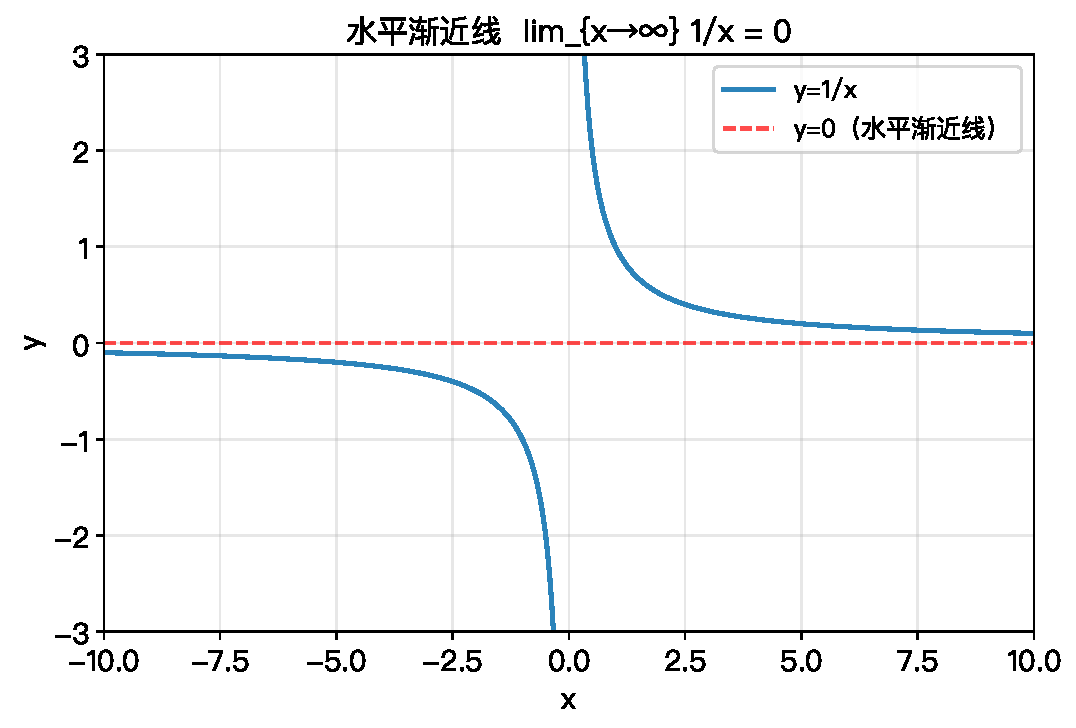
\includegraphics[width=0.7\textwidth]{figures/ch13_horizontal_asymptote.pdf}
\end{center}

\[
\lim_{x \to \infty} \frac{1}{x} = 0,\qquad
\lim_{x \to -\infty} \frac{1}{x} = 0
\]

\textbf{几何意义：} 直线 \(y = 0\) 是函数的\textbf{水平渐近线}。
当 \(x\) 趋向无穷时，曲线无限接近这条线，但永远不碰到（\(x\) 有限时）。
\end{examplebox}


% ============================================================
\section{不同函数的增长速度}
% ============================================================

\begin{examplebox}[2——增长速度的"等级"]
\begin{center}
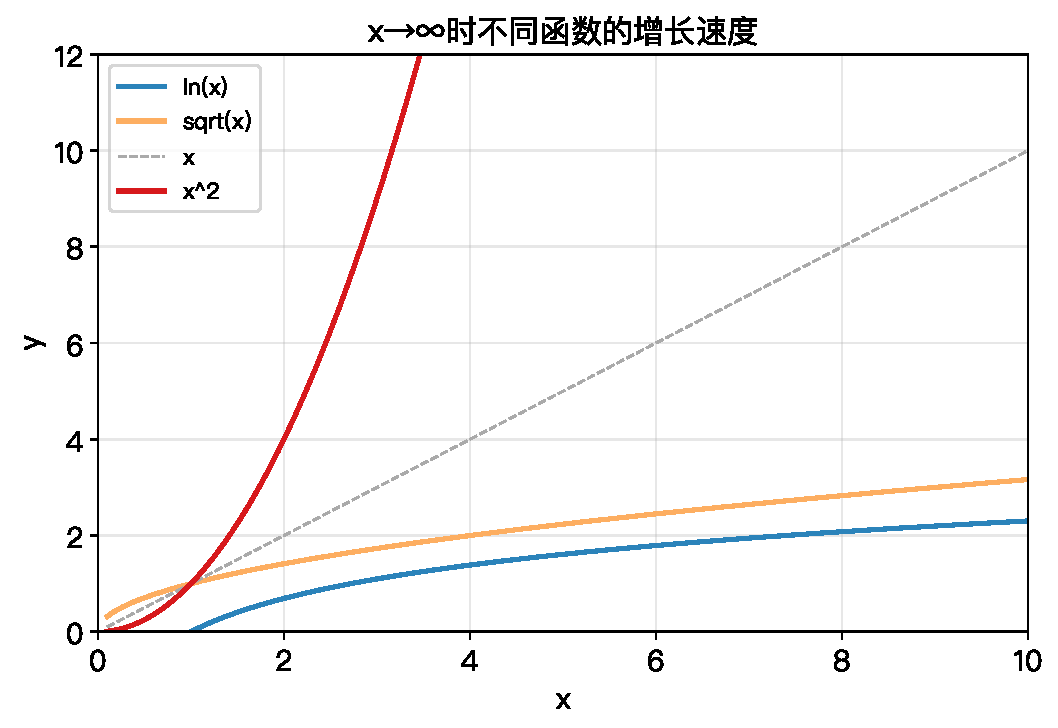
\includegraphics[width=0.7\textwidth]{figures/ch13_growth_rates.pdf}
\end{center}

当 \(x \to \infty\) 时，增长速度从慢到快：
\[
\ln x \;\ll\; \sqrt{x} \;\ll\; x \;\ll\; x^2 \;\ll\; x^3 \;\ll\; e^x \;\ll\; 2^x
\]

\textbf{重要结论：}
\begin{itemize}
  \item 对数增长最慢（\(\ln x\)）
  \item 幂函数 \(x^k\) 按指数 \(k\) 分等级
  \item 指数函数 \(e^x\) 碾压所有幂函数
\end{itemize}
\end{examplebox}


% ============================================================
\section{\(x \to a\) 时的无穷极限}
% ============================================================

\begin{definitionbox}[无穷极限]
如果当 \(x\) 趋近于 \(a\) 时，\(f(x)\) 的绝对值无限增大，
则称 \(f(x)\) 在 \(x=a\) 处\textbf{趋于无穷}。

记作 \(\displaystyle \lim_{x \to a} f(x) = \infty\)（或 \(-\infty\)），此时 \(x=a\) 是\textbf{垂直渐近线}。

\textbf{ε-δ 定义：} 对任意 \(M>0\)，存在 \(\delta>0\)，使得当 \(0<|x-a|<\delta\) 时，
\(f(x) > M\)（或 \(f(x) < -M\)）。
\end{definitionbox}

\begin{examplebox}[3——垂直渐近线]
\begin{center}
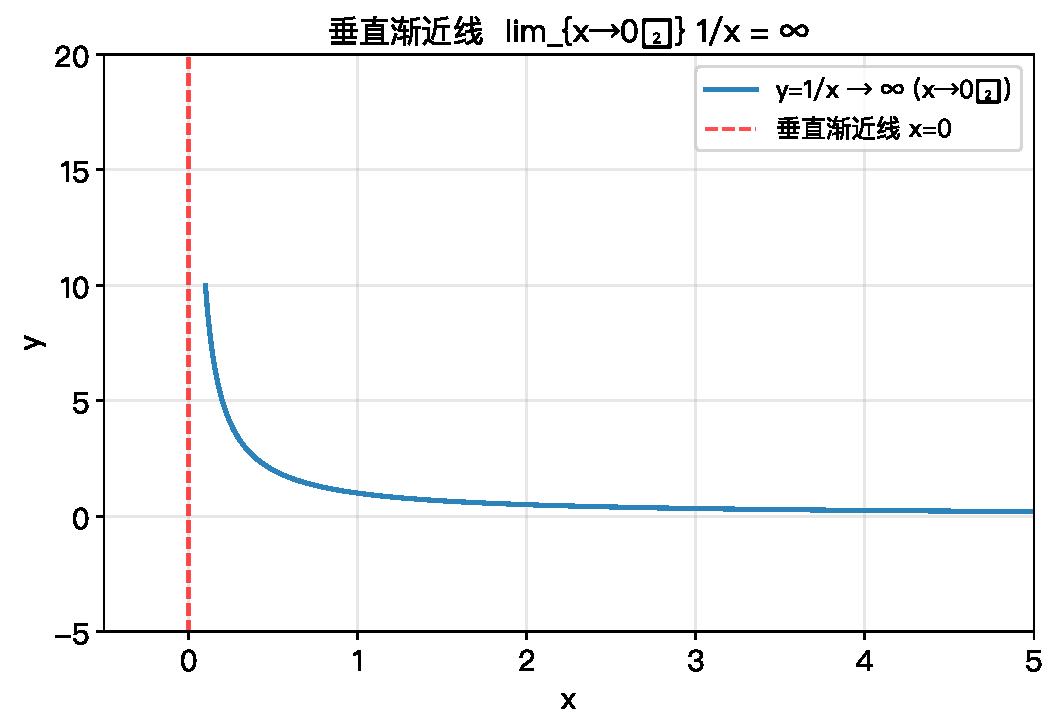
\includegraphics[width=0.7\textwidth]{figures/ch13_vertical_asymptote.pdf}
\end{center}

\[
\lim_{x \to 0^+} \frac{1}{x} = +\infty,\qquad
\lim_{x \to 0^-} \frac{1}{x} = -\infty
\]

\(x = 0\) 是 \(y = 1/x\) 的\textbf{垂直渐近线}。
当 \(x\) 从右侧趋近 0 时，函数值趋向正无穷；
从左侧趋近 0 时，函数值趋向负无穷。
\end{examplebox}


% ============================================================
\section{本章小结}
% ============================================================

\begin{progressbox}
\textbf{函数在无穷远处的极限}：\(\lim_{x \to \infty} f(x) = L\) 对应水平渐近线 \(y = L\)

\textbf{无穷极限}：\(\lim_{x \to a} f(x) = \infty\) 对应垂直渐近线 \(x = a\)

\textbf{增长速度等级}：\(\ln x < \sqrt{x} < x < x^2 < x^3 < e^x\)
\end{progressbox}


% ============================================================
% 习题
% ============================================================
\section{习题}

\begin{exercise}[0]
求 \(\displaystyle\lim_{x\to\infty} \frac{1}{x}\)。
\end{exercise}
\begin{exercise}[0]
函数 \(y=1/x\) 的水平渐近线是什么？
\end{exercise}
\begin{exercise}[0]
函数 \(y=1/x\) 的垂直渐近线是什么？
\end{exercise}
\begin{exercise}[0]
判断：\(\displaystyle\lim_{x\to\infty} e^x\) 是有限数吗？
\end{exercise}

\begin{exercise}[1]
求 \(\displaystyle\lim_{x\to\infty} \frac{2}{x+1}\)。
\end{exercise}
\begin{exercise}[1]
求 \(\displaystyle\lim_{x\to-\infty} \frac{1}{x^2}\)。
\end{exercise}
\begin{exercise}[1]
比较大小（\(x\) 很大时）：\(x^{100}\) 和 \(1.001^x\) 哪个增长更快？
\end{exercise}
\begin{exercise}[1]
判断：若 \(\lim_{x\to\infty} f(x)=5\)，则 \(y=5\) 是一条什么线？
\end{exercise}

\begin{exercise}[2]
求 \(\displaystyle\lim_{x\to\infty} \frac{2x+1}{x-3}\)。
\end{exercise}
\begin{exercise}[2]
求 \(\displaystyle\lim_{x\to\infty} \frac{x^2+1}{3x^2-2x}\)。
\end{exercise}
\begin{exercise}[2]
求 \(\displaystyle\lim_{x\to 0^+} \ln x\)（提示：\(\ln x \to -\infty\)）。
\end{exercise}
\begin{exercise}[2]
函数 \(y=\frac{1}{(x-2)^2}\) 的垂直渐近线在哪里？
\end{exercise}

\begin{exercise}[3]
求 \(\displaystyle\lim_{x\to\infty} (\sqrt{x+1}-\sqrt{x})\)。
\end{exercise}
\begin{exercise}[3]
求水平渐近线：\(y=\frac{2x^2+1}{x^2-4}\)。
\end{exercise}
\begin{exercise}[3]
求垂直渐近线：\(y=\frac{x}{x^2-1}\)。
\end{exercise}
\begin{exercise}[3]
比较 \(\lim_{x\to\infty} \frac{x^{10}}{2^x}\) 和 \(\lim_{x\to\infty} \frac{2^x}{x^{10}}\)。
\end{exercise}
\begin{exercise}[3]
某药的血药浓度 \(C(t)=\frac{100t}{t+2}\)，求 \(t\to\infty\) 时的极限浓度。
\end{exercise}

\begin{exercise}[4]
求 \(\displaystyle\lim_{x\to\infty} \left(\frac{x+1}{x-1}\right)^x\)。
\end{exercise}
\begin{exercise}[4]
证明 \(\displaystyle\lim_{x\to\infty} \frac{\ln x}{x} = 0\)。
\end{exercise}
\begin{exercise}[4]
求渐近线：\(y=\frac{x^2+1}{x}\)（提示：有斜渐近线）。
\end{exercise}
\begin{exercise}[4]
函数 \(f(x)=\frac{e^x}{e^x+1}\)，求水平渐近线。
\end{exercise}
\begin{exercise}[4]
求 \(\displaystyle\lim_{x\to\infty} \frac{\sin x}{x}\)。
\end{exercise}

\begin{exercise}[5]
证明 \(\displaystyle\lim_{x\to\infty} \frac{x^k}{e^x}=0\) 对任意正整数 \(k\) 成立。
\end{exercise}
\begin{exercise}[5]
求 \(\displaystyle\lim_{x\to 0} \frac{1}{x^2}\) 并从左右两侧讨论。
\end{exercise}
\begin{exercise}[5]
函数 \(y=\frac{2x^2+3x+1}{x^2-5x+6}\) 的水平和垂直渐近线。
\end{exercise}
\begin{exercise}[5]
求 \(\displaystyle\lim_{x\to\infty} x\sin\frac{1}{x}\)。
\end{exercise}

\begin{exercise}[6]
证明 \(\displaystyle\lim_{x\to\infty} \left(1+\frac{1}{x}\right)^x = e\)。
\end{exercise}
\begin{exercise}[6]
求 \(\displaystyle\lim_{x\to 0^+} x\ln x\)。
\end{exercise}
\begin{exercise}[6]
求 \(\displaystyle\lim_{x\to\infty} \frac{\ln(1+e^x)}{x}\)。
\end{exercise}

\begin{exercise}[7]
设 \(f(x)=\frac{x^n}{e^x}\)（\(n\) 为正整数）。
\begin{enumerate}
  \item[(1)] 证明存在 \(X\) 使 \(x>X\) 时 \(f(x)<\frac{1}{x}\)
  \item[(2)] 求 \(\lim_{x\to\infty} f(x)\)
\end{enumerate}
\end{exercise}


% ============================================================
% 第14章：函数在一点处的极限——ε-δ 定义
% ============================================================

\chapter{函数在一点处的极限——ε-δ 定义}

\begin{applicationbox}
\textbf{学完本章你能做什么？}
\begin{enumerate}
  \item 理解函数在一点处极限的 \textbf{ε-δ 定义}
  \item 掌握左右极限的概念——从左侧和右侧趋近
  \item 用 ε-δ 证明简单的函数极限
\end{enumerate}
\end{applicationbox}


% ============================================================
\section{从 \(x \to \infty\) 到 \(x \to a\)}
% ============================================================

第13章我们学了 \(x \to \infty\) 时的极限——函数在无穷远处的行为。

现在问一个更基本的问题：当 \(x\) 趋近于一个\textbf{有限数 \(a\)} 时，\(f(x)\) 会怎样？

\[
\lim_{x \to a} f(x) = L
\]

\textbf{含义：} 当 \(x\) 越来越接近 \(a\)（但不等于 \(a\)）时，\(f(x)\) 越来越接近 \(L\)。

\begin{examplebox}[1——直观例子]
\[
f(x) = 2x + 1,\quad \lim_{x \to 2} f(x) = 5
\]

验证：
\[
x=1.9 \to f=4.8,\; x=1.99 \to f=4.98,\; x=1.999 \to f=4.998
\]
\[
x=2.1 \to f=5.2,\; x=2.01 \to f=5.02,\; x=2.001 \to f=5.002
\]

不管从左边还是右边靠近 2，\(f(x)\) 都靠近 5。
\end{examplebox}


% ============================================================
\section{ε-δ 定义}
% ============================================================

\begin{definitionbox}[函数极限的 ε-δ 定义]
设 \(f(x)\) 在 \(x=a\) 的某个去心邻域内有定义。
如果对\textbf{任意} \(\varepsilon > 0\)，都\textbf{存在} \(\delta > 0\)，
使得当 \(0 < |x - a| < \delta\) 时，有
\[
|f(x) - L| < \varepsilon
\]
则称 \(\displaystyle \lim_{x \to a} f(x) = L\)。
\end{definitionbox}

\begin{examplebox}[2——ε-δ 的几何意义]
\begin{center}
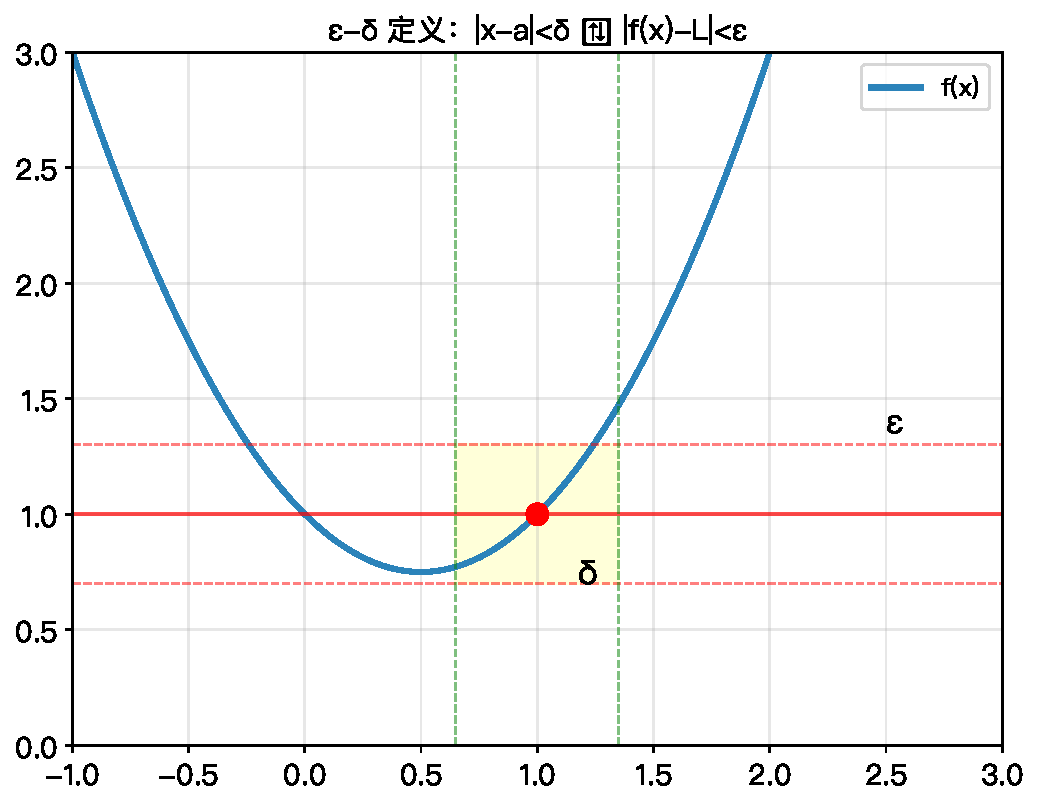
\includegraphics[width=0.7\textwidth]{figures/ch14_epsilon_delta.pdf}
\end{center}

\textbf{解读：}
\begin{itemize}
  \item 给你一个 \(\varepsilon\)（对 \(y\) 方向的精度要求）
  \item 我找到一个 \(\delta\)（\(x\) 方向的范围）
  \item 只要 \(x\) 在 \(a\) 的 \(\delta\) 邻域内（但不等于 \(a\)）
  \item \(f(x)\) 就一定在 \(L\) 的 \(\varepsilon\) 邻域内
\end{itemize}
\end{examplebox}


% ============================================================
\section{左右极限}
% ============================================================

\begin{definitionbox}[左右极限]
\begin{itemize}
  \item \textbf{左极限}：\(x\) 从左侧趋近 \(a\)（\(x \to a^-\)），记 \(\displaystyle \lim_{x \to a^-} f(x)\)
  \item \textbf{右极限}：\(x\) 从右侧趋近 \(a\)（\(x \to a^+\)），记 \(\displaystyle \lim_{x \to a^+} f(x)\)
\end{itemize}

极限存在的\textbf{充要条件}：左右极限都存在且相等。
\end{definitionbox}

\begin{examplebox}[3——左右极限不相等]
\[
f(x) = 
\begin{cases}
x + 1, & x \ge 0 \\
x - 1, & x < 0
\end{cases}
\]

\[
\lim_{x \to 0^+} f(x) = 1,\qquad
\lim_{x \to 0^-} f(x) = -1
\]

左右极限不相等 \(\Rightarrow\) \(\displaystyle\lim_{x \to 0} f(x)\) 不存在。
\end{examplebox}


% ============================================================
\section{本章小结}
% ============================================================

\begin{progressbox}
\textbf{ε-δ 定义}：\(\forall\varepsilon>0,\exists\delta>0\) 使 \(0<|x-a|<\delta \Rightarrow |f(x)-L|<\varepsilon\)

\textbf{左右极限}：\(x \to a^-\)（左）和 \(x \to a^+\)（右）\\
极限存在 \(\iff\) 左右极限存在且相等
\end{progressbox}

% ============================================================
% 习题
% ============================================================
\section{习题}

\begin{exercise}[0]
求 \(\displaystyle\lim_{x\to 1} (2x+1)\)。
\end{exercise}
\begin{exercise}[0]
判断：\(\displaystyle\lim_{x\to 0} \frac{|x|}{x}\) 存在吗？
\end{exercise}
\begin{exercise}[0]
若左右极限不相等，极限存在吗？
\end{exercise}
\begin{exercise}[0]
\(\varepsilon\)-\(\delta\) 定义中，\(\varepsilon\) 和 \(\delta\) 哪个先给？
\end{exercise}

\begin{exercise}[1]
求 \(\displaystyle\lim_{x\to 3} (x^2-1)\)。
\end{exercise}
\begin{exercise}[1]
求 \(\displaystyle\lim_{x\to 0^-} \frac{1}{x}\)。
\end{exercise}
\begin{exercise}[1]
求 \(\displaystyle\lim_{x\to 0^+} \frac{1}{x}\)。
\end{exercise}
\begin{exercise}[1]
判断：\(\displaystyle\lim_{x\to 0} \frac{1}{x}\) 存在吗？
\end{exercise}

\begin{exercise}[2]
已知 \(f(x)=\frac{x^2-1}{x-1}\)（\(x\neq1\)），求 \(\lim_{x\to 1} f(x)\)。
\end{exercise}
\begin{exercise}[2]
求 \(\displaystyle\lim_{x\to 2} \frac{x^2-4}{x-2}\)。
\end{exercise}
\begin{exercise}[2]
设 \(f(x)=\begin{cases}x^2,&x\ge1\\2x-1,&x<1\end{cases}\)，求左右极限和极限。
\end{exercise}
\begin{exercise}[2]
用 ε-δ 语言写出 \(\lim_{x\to 2} (3x-1)=5\) 的证明框架。
\end{exercise}

\begin{exercise}[3]
计算 \(\displaystyle\lim_{x\to 0} \frac{\sin x}{x}\)（查计算器取 \(x=0.1,0.01,0.001\)）。
\end{exercise}
\begin{exercise}[3]
求 \(\displaystyle\lim_{x\to 4} \frac{\sqrt{x}-2}{x-4}\)。
\end{exercise}
\begin{exercise}[3]
已知 \(\lim_{x\to a} f(x)=L\)，用 ε-δ 语言证明 \(\lim_{x\to a} cf(x)=cL\)。
\end{exercise}
\begin{exercise}[3]
讨论 \(\displaystyle\lim_{x\to 0} \frac{1}{x^2}\) 是否存在。
\end{exercise}
\begin{exercise}[3]
若 \(\lim_{x\to a} f(x)=L\)，\(\lim_{x\to a} g(x)=M\)，证明 \(\lim_{x\to a} [f(x)+g(x)]=L+M\)。
\end{exercise}

\begin{exercise}[4]
用 ε-δ 语言证明 \(\displaystyle\lim_{x\to 2} (x^2-3x+1)=-1\)。
\end{exercise}
\begin{exercise}[4]
讨论 \(\displaystyle\lim_{x\to 0} \frac{1}{x}\sin\frac{1}{x}\) 是否存在。
\end{exercise}
\begin{exercise}[4]
证明：若 \(\lim_{x\to a} f(x)=L>0\)，则存在 \(\delta>0\) 使 \(0<|x-a|<\delta\) 时 \(f(x)>0\)。
\end{exercise}
\begin{exercise}[4]
求 \(\displaystyle\lim_{x\to 0} \frac{\tan x}{x}\)。
\end{exercise}
\begin{exercise}[4]
设 \(f(x)=\begin{cases}x\sin\frac1x,&x\neq0\\0,&x=0\end{cases}\)，讨论 \(\lim_{x\to0} f(x)\)。
\end{exercise}

\begin{exercise}[5]
用 ε-δ 语言证明 \(\displaystyle\lim_{x\to 1} \frac{1}{x}=1\)。
\end{exercise}
\begin{exercise}[5]
证明：若 \(\lim_{x\to a} f(x)=L\)，则 \(\lim_{x\to a} |f(x)|=|L|\)。
\end{exercise}
\begin{exercise}[5]
求 \(\displaystyle\lim_{x\to 0} \frac{\sqrt{1+x}-1}{x}\)。
\end{exercise}
\begin{exercise}[5]
求 \(\displaystyle\lim_{x\to 0} \frac{e^x-1}{x}\)。
\end{exercise}

\begin{exercise}[6]
用 ε-δ 语言证明 \(\displaystyle\lim_{x\to a} x^2=a^2\)。
\end{exercise}
\begin{exercise}[6]
证明极限的唯一性：若 \(\lim_{x\to a} f(x)=L\) 且 \(\lim_{x\to a} f(x)=M\)，则 \(L=M\)。
\end{exercise}
\begin{exercise}[6]
求 \(\displaystyle\lim_{x\to 0} \frac{\ln(1+x)}{x}\)。
\end{exercise}

\begin{exercise}[7]
用 ε-δ 语言证明：若 \(\lim_{x\to a} f(x)=L\)，\(\lim_{x\to a} g(x)=M\)，
则 \(\lim_{x\to a} f(x)g(x)=LM\)。
\end{exercise}


% ============================================================
% 第15章：连续函数——一笔画
% ============================================================

\chapter{连续函数——从极限到连续}

\begin{applicationbox}
\textbf{学完本章你能做什么？}
\begin{enumerate}
  \item 理解\textbf{连续}的严格定义——极限等于函数值
  \item 能判断函数在一点处是否连续
  \item 能分类\textbf{间断点}——可去、跳跃、无穷、振荡
\end{enumerate}
\end{applicationbox}


% ============================================================
\section{从极限到连续}
% ============================================================

极限研究的是 \(x \to a\) 时 \(f(x)\) 趋近于什么——不关心 \(x=a\) 处的值。

连续则要求：\textbf{极限值等于函数值}。

\begin{definitionbox}[连续的定义]
函数 \(f\) 在 \(x=a\) 处\textbf{连续}，如果：
\[
\lim_{x \to a} f(x) = f(a)
\]

用 ε-δ 语言：对任意 \(\varepsilon > 0\)，存在 \(\delta > 0\)，
使得 \(|x-a| < \delta\) 时 \(|f(x) - f(a)| < \varepsilon\)。
\end{definitionbox}

\begin{examplebox}[1——连续 vs 间断]
\begin{center}
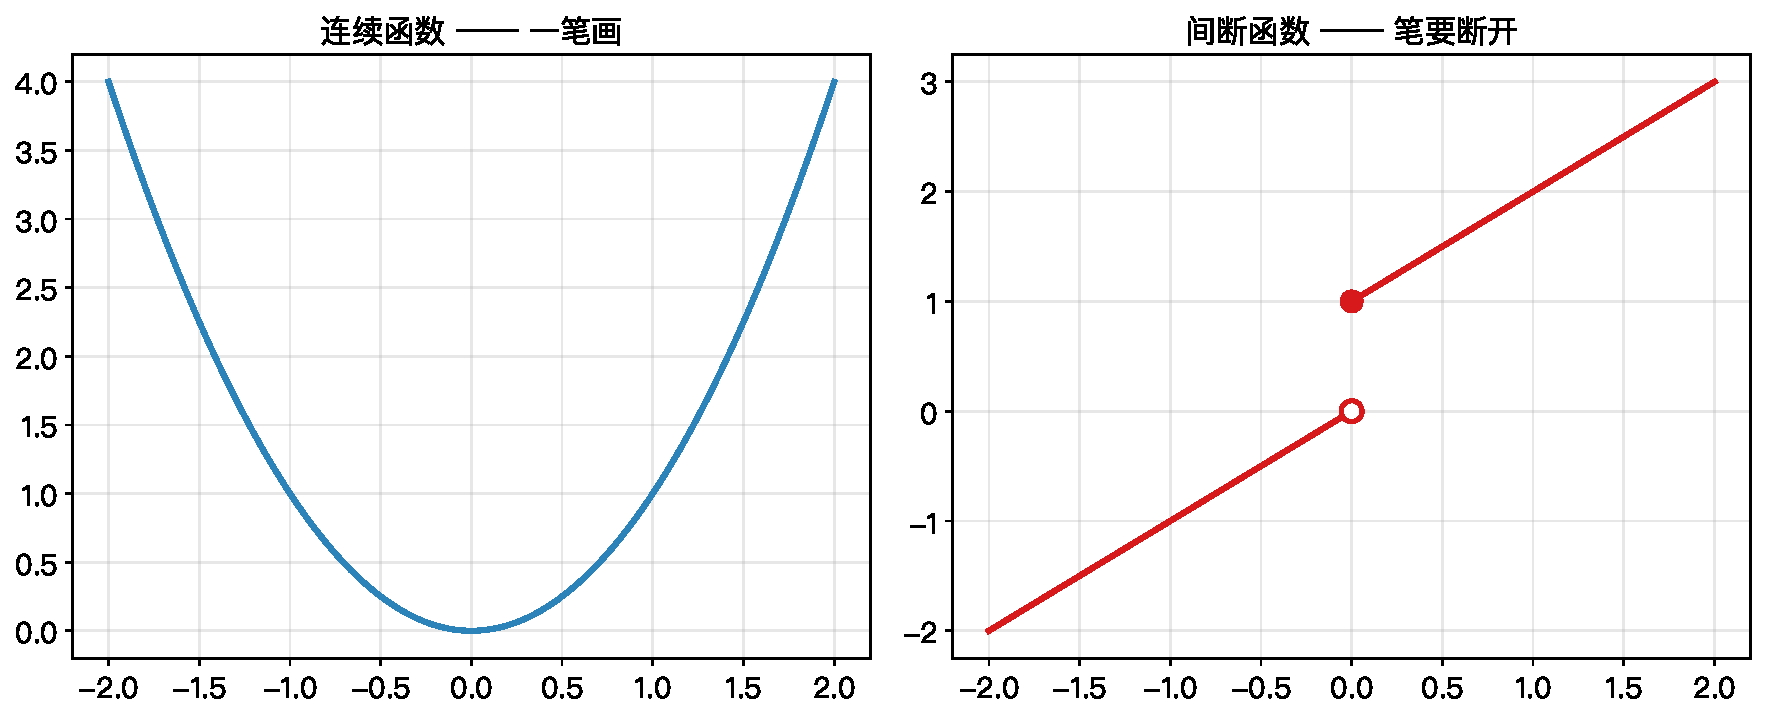
\includegraphics[width=0.85\textwidth]{figures/ch15_continuous_vs_discontinuous.pdf}
\end{center}

\textbf{左图：} \(y = x^2\)——在 \(x=0\) 处连续（\(\lim_{x\to0} x^2 = 0 = f(0)\)）\\
\textbf{右图：} 分段函数在 \(x=0\) 处间断——左右极限不等
\end{examplebox}


% ============================================================
\section{间断点的分类}
% ============================================================

\begin{definitionbox}[间断点分类]
\begin{center}
\begin{tabular}{c|c|c}
\textbf{类型} & \textbf{特征} & \textbf{例子} \\
\hline
\textbf{可去间断点} & 极限存在但不等于函数值 & \(y=\frac{x^2-1}{x-1}\) 在 \(x=1\) \\
\textbf{跳跃间断点} & 左右极限存在但不相等 & \(y=\frac{|x|}{x}\) 在 \(x=0\) \\
\textbf{无穷间断点} & 极限为无穷大 & \(y=\frac{1}{x}\) 在 \(x=0\) \\
\textbf{振荡间断点} & 极限不存在（振荡） & \(y=\sin\frac{1}{x}\) 在 \(x=0\) \\
\end{tabular}
\end{center}
\end{definitionbox}


% ============================================================
\section{本章小结}
% ============================================================

\begin{progressbox}
\textbf{连续}：\(\lim_{x\to a} f(x) = f(a)\)——极限等于函数值

\textbf{间断点}：可去、跳跃、无穷、振荡四种

初等函数在其定义域内都是连续的
\end{progressbox}


% ============================================================
\section{邻域语言——从 ε-δ 到开集}
% ============================================================

ε-δ 语言精确但繁琐。每次写"存在 δ>0 使 |x-a|<δ"很重复。
**邻域语言**把 ε-δ 的核心操作封装成更抽象的词汇。

\subsection{ε-邻域}

\begin{definitionbox}[邻域]
设 \(a\in\mathbb{R}\)，\(\varepsilon>0\)。称区间 \((a-\varepsilon, a+\varepsilon)\) 为 \(a\) 的
\textbf{ε-邻域}（读作 lín yù，英文 neighborhood），记作 \(U(a,\varepsilon)\)。

\[
U(a,\varepsilon) = \{x\in\mathbb{R}: |x-a|<\varepsilon\}
\]
\end{definitionbox}

用邻域语言翻译 ε-δ 定义：

\begin{center}
\fcolorbox{green!30}{green!5}{\parbox{0.85\textwidth}{
\(\displaystyle\lim_{x\to a}f(x)=L\) 的意思是：\\
对 \(L\) 的任意邻域 \(U(L,\varepsilon)\)，存在 \(a\) 的邻域 \(U(a,\delta)\)，
使得 \(f(U(a,\delta)\setminus\{a\}) \subseteq U(L,\varepsilon)\)。
}}
\end{center}

这比"对任意 ε>0 存在 δ>0 使得……"更紧凑，而且可以推广到高维空间。

\subsection{开集与闭集}

\begin{definitionbox}[开集与闭集]
\begin{itemize}
  \item \(U\subset\mathbb{R}\) 称为\textbf{开集}（open set），如果 \(U\) 中每一点都有一个
        完全包含在 \(U\) 内的邻域。
  \item \(F\subset\mathbb{R}\) 称为\textbf{闭集}（closed set），如果它的补集 \(\mathbb{R}\setminus F\) 是开集。
\end{itemize}
\end{definitionbox}

\begin{examplebox}[8——开集和闭集的例子]
\begin{itemize}
  \item \((a,b)\) 是开集（每点都能找到 ε 邻域不碰边界）
  \item \([a,b]\) 是闭集（补集 \((-\infty,a)\cup(b,\infty)\) 是开集）
  \item \(\mathbb{R}\) 既是开集也是闭集
  \item 有限个点的集合是闭集
\end{itemize}
\end{examplebox}

\subsection{开覆盖与紧致性}

\begin{definitionbox}[开覆盖]
设 \(S\subset\mathbb{R}\)。一族开集 \(\{U_i\}_{i\in I}\) 称为 \(S\) 的\textbf{开覆盖}（open cover），
如果 \(S\subset\bigcup_{i\in I}U_i\)。如果其中有限个开集已经能覆盖 \(S\)，
则称有\textbf{有限子覆盖}。
\end{definitionbox}

\begin{theorembox}[海涅-博雷尔定理]
闭区间 \([a,b]\) 的任意开覆盖都有有限子覆盖。
这是实数完备性的重要体现，也是数学分析中"有限覆盖引理"的来源。
\end{theorembox}

这个定理的严格证明需要实数完备性（确界定理），此处先作为引理接受。
有了它，ch16 中有界性定理的证明就不再是空中楼阁。

\subsection{翻译对照表}

\begin{center}
\begin{tabular}{c|c}
\textbf{ε-δ 语言} & \textbf{邻域语言} \\
\hline
\(|x-a|<\delta\) & \(x\in U(a,\delta)\) \\
\(a\) 是聚点 & 任意去心邻域包含 \(S\) 中的点 \\
\(f\) 连续 & 开集的原像是开集 \\
一致连续 & \(\delta\) 与 \(x\) 无关 \\
开覆盖 & 一族开集覆盖了区间 \\
有限子覆盖 & 其中有限个就够了 \\
\end{tabular}
\end{center}

邻域语言是连接 ε-δ 分析和一般拓扑学的桥梁。在实分析中，常用 ε-δ；
在泛函分析和拓扑学中，用开集语言。两者是等价的描述方式。

% ============================================================
% 习题
% ============================================================
\section{习题}

\begin{exercise}[0]
函数 \(f(x)=x^2\) 在 \(x=2\) 处连续吗？
\end{exercise}
\begin{exercise}[0]
判断：\(f(x)=\frac{1}{x}\) 在 \(x=0\) 处连续吗？
\end{exercise}
\begin{exercise}[0]
可去间断点的左右极限相等吗？
\end{exercise}
\begin{exercise}[0]
跳跃间断点的左右极限存在吗？
\end{exercise}

\begin{exercise}[1]
求 \(f(x)=\frac{x^2-9}{x-3}\) 在 \(x=3\) 处的极限，它是可去间断点吗？
\end{exercise}
\begin{exercise}[1]
\(y=\frac{1}{x}\) 在 \(x=0\) 处是什么类型的间断点？
\end{exercise}
\begin{exercise}[1]
\(y=\frac{|x|}{x}\) 在 \(x=0\) 处是什么类型的间断点？
\end{exercise}
\begin{exercise}[1]
判断：多项式函数在其定义域内是否连续？
\end{exercise}

\begin{exercise}[2]
确定 \(f(x)=\frac{x^2-1}{x^2-3x+2}\) 的间断点并分类。
\end{exercise}
\begin{exercise}[2]
设 \(f(x)=\begin{cases}x^2,&x\ge0\\x+1,&x<0\end{cases}\)，判断 \(x=0\) 处的连续性。
\end{exercise}
\begin{exercise}[2]
求 \(k\) 使 \(f(x)=\begin{cases}x^2,&x\le1\\kx,&x>1\end{cases}\) 在 \(x=1\) 处连续。
\end{exercise}
\begin{exercise}[2]
证明 \(f(x)=x^2\) 在 \(x=3\) 处连续（用 ε-δ）。
\end{exercise}

\begin{exercise}[3]
证明 \(f(x)=\sqrt{x}\) 在 \(x=4\) 处连续。
\end{exercise}
\begin{exercise}[3]
\(y=\sin\frac{1}{x}\) 在 \(x=0\) 处是什么类型的间断点？
\end{exercise}
\begin{exercise}[3]
设 \(f(x)=\begin{cases}\frac{\sin x}{x},&x\neq0\\1,&x=0\end{cases}\)，判断 \(x=0\) 处的连续性。
\end{exercise}
\begin{exercise}[3]
\(f(x)=\frac{1}{x^2}\) 在 \(x=0\) 处是什么类型的间断点？
\end{exercise}
\begin{exercise}[3]
证明：若 \(f\) 在 \(x=a\) 处连续，则 \(|f|\) 也在 \(x=a\) 处连续。
\end{exercise}

\begin{exercise}[4]
证明：\(f(x)=x^3\) 在任意点 \(x=a\) 处连续。
\end{exercise}
\begin{exercise}[4]
讨论 \(f(x)=\begin{cases}x\sin\frac1x,&x\neq0\\0,&x=0\end{cases}\) 在 \(x=0\) 处的连续性。
\end{exercise}
\begin{exercise}[4]
证明：若 \(f\) 在 \(x=a\) 处连续，则 \(f^2\) 也在 \(x=a\) 处连续。
\end{exercise}
\begin{exercise}[4]
设 \(f(x)=\frac{1}{1+e^{1/x}}\)（\(x\neq0\)），讨论 \(x=0\) 处的左右极限和连续性。
\end{exercise}
\begin{exercise}[4]
判断 \(f(x)=\lfloor x\rfloor\)（取整函数）的间断点并分类。
\end{exercise}

\begin{exercise}[5]
证明 \(f(x)=\sin x\) 在任意点处连续。
\end{exercise}
\begin{exercise}[5]
设 \(f(x)=\begin{cases}e^{-1/x^2},&x\neq0\\0,&x=0\end{cases}\)，证明 \(f\) 在 \(x=0\) 处连续。
\end{exercise}
\begin{exercise}[5]
判断 \(f(x)=\tan x\) 的间断点并分类。
\end{exercise}
\begin{exercise}[5]
已知 \(f\) 在 \(x=a\) 处连续，证明 \(f_+(x)=\max(f(x),0)\) 也在 \(x=a\) 处连续。
\end{exercise}

\begin{exercise}[6]
证明黎曼函数 \(R(x)=\begin{cases}1/q,&x=p/q\\0,&x\text{无理数}\end{cases}\) 在无理点连续，在有理点间断。
\end{exercise}
\begin{exercise}[6]
若 \(f\) 在 \(x=a\) 处连续且 \(f(a)>0\)，证明存在 \(\delta>0\) 使 \(|x-a|<\delta\) 时 \(f(x)>0\)。
\end{exercise}
\begin{exercise}[6]
构造一个在 \(\mathbb{R}\) 上处处不连续的函数的例子。
\end{exercise}

\begin{exercise}[7]
证明：若 \(f\) 在 \([a,b]\) 上连续且严格递增，则 \(f\) 的值域是 \([f(a),f(b)]\)。
\end{exercise}


% ============================================================
% 第16章：闭区间上连续函数的性质——四大定理
% ============================================================

\chapter{闭区间上连续函数的性质——四大定理}

\begin{applicationbox}
\textbf{学完本章你能做什么？}
\begin{enumerate}
  \item 掌握闭区间上连续函数的\textbf{四大定理}
  \item 理解\textbf{介值定理}——中间值一定有解
  \item 理解\textbf{最值定理}——闭区间上一定有最大值和最小值
\end{enumerate}
\end{applicationbox}


% ============================================================
\section{四大定理}
% ============================================================

\begin{theorembox}[1. 有界性定理]
若 \(f\) 在 \([a,b]\) 上连续，则 \(f\) 在 \([a,b]\) 上有界。

\textbf{ε-δ 证明：} 由 \(f\) 在 \([a,b]\) 上 ε-δ 连续（第15章），
取 \(\varepsilon=1\)，则对每个 \(x\in[a,b]\)，存在 \(\delta_x>0\) 使
\(|y-x|<\delta_x\) 时 \(|f(y)-f(x)|<1\)。
开区间族 \(\{U(x,\delta_x)\}_{x\in[a,b]}\)（即 \((x-\delta_x,x+\delta_x)\)）构成 \([a,b]\) 的开覆盖。
由海涅-博雷尔定理（第15章第5.3节），存在有限子覆盖 \(U(x_1,\delta_{x_1}),\ldots,U(x_n,\delta_{x_n})\)。
取 \(M=\max\{|f(x_1)|,\ldots,|f(x_n)|\}+1\)，则对任意 \(y\in[a,b]\)，
\(y\) 属于某个 \(U(x_i,\delta_{x_i})\)，故 \(|f(y)|\le|f(x_i)|+1\le M\)，即 \(f\) 有界。\(\blacksquare\)
\end{theorembox}

\begin{theorembox}[2. 最值定理（最大值最小值定理）]
若 \(f\) 在 \([a,b]\) 上连续，则 \(f\) 在 \([a,b]\) 上一定能取到最大值和最小值。

\textbf{ε-δ 证明：} 由有界性定理知 \(f\) 有上确界 \(M=\sup\{f(x):x\in[a,b]\}\)。
假设 \(f(x)<M\) 对所有 \(x\in[a,b]\) 成立，则 \(g(x)=\frac1{M-f(x)}\) 在 \([a,b]\) 上 ε-δ 连续（分母不为 0）。
但 \(g(x)\) 无界（因为 \(f(x)\) 可任意接近 \(M\)），与有界性定理矛盾。
故存在 \(c\) 使 \(f(c)=M\)，即最大值可达。最小值同理。\(\blacksquare\)
\end{theorembox}

\begin{theorembox}[3. 介值定理]
若 \(f\) 在 \([a,b]\) 上连续，且 \(f(a) \neq f(b)\)，
则对 \(f(a)\) 和 \(f(b)\) 之间的任意数 \(k\)，
存在 \(c \in (a,b)\) 使得 \(f(c) = k\)。

\textbf{ε-δ 证明：} 设 \(f(a)<k<f(b)\)。令集合 \(S=\{x\in[a,b]:f(x)<k\}\)，
则 \(S\) 非空（\(a\in S\)），有上界（\(b\) 为上界）。设 \(c=\sup S\)（上确界）。
由 \(f\) 的 ε-δ 连续性，若 \(f(c)<k\)，则存在 \(\delta>0\) 使
\((c,c+\delta)\) 内 \(f(x)<k\)，与 \(c\) 是上界矛盾；
若 \(f(c)>k\)，则存在 \(\delta>0\) 使 \((c-\delta,c+\delta)\) 内 \(f(x)>k\)，
与 \(c\) 是上确界矛盾。故 \(f(c)=k\)。\(\blacksquare\)
\end{theorembox}

\begin{theorembox}[4. 零点定理（介值定理的推论）]
若 \(f\) 在 \([a,b]\) 上连续，且 \(f(a) \cdot f(b) < 0\)（即一正一负），
则存在 \(c \in (a,b)\) 使得 \(f(c) = 0\)。
\end{theorembox}


% ============================================================
\section{介值定理的几何意义}
% ============================================================

\begin{examplebox}[1——介值定理]
\begin{center}
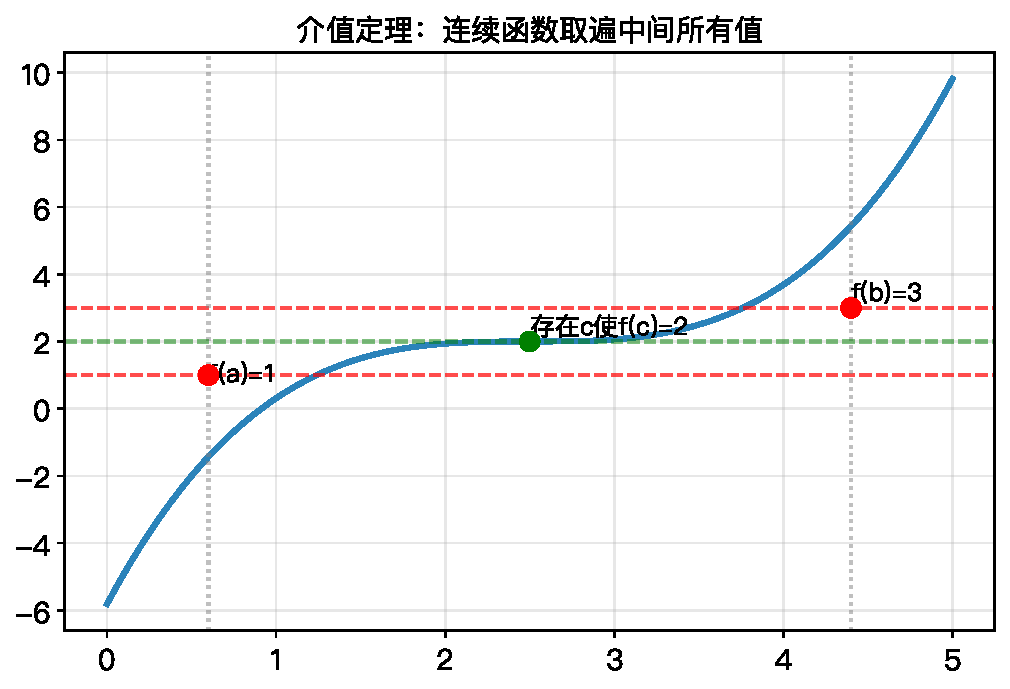
\includegraphics[width=0.7\textwidth]{figures/ch16_intermediate_value.pdf}
\end{center}

连续函数的图像从 \(f(a)=1\) 到 \(f(b)=3\)，中间不能断开，\
所以一定会经过 \(y=2\)。这就是介值定理——连续函数取遍中间所有值。
\end{examplebox}

\begin{examplebox}[2——零点定理的应用]
证明方程 \(x^3 - x - 1 = 0\) 在 \((1,2)\) 内有根。

\textbf{证明：} 令 \(f(x) = x^3 - x - 1\)。\\
\(f(1) = 1 - 1 - 1 = -1 < 0\)\\
\(f(2) = 8 - 2 - 1 = 5 > 0\)

\(f\) 在 \([1,2]\) 上连续，且 \(f(1)f(2) < 0\)。\\
由零点定理，存在 \(c \in (1,2)\) 使得 \(f(c) = 0\)，即 \(c\) 是方程的根。
\end{examplebox}


% ============================================================
\section{本章小结}
% ============================================================

\begin{progressbox}
\textbf{闭区间上连续函数的四大定理：}
\begin{itemize}
  \item 有界性定理：连续必有界
  \item 最值定理：连续必取最值
  \item 介值定理：连续必取中间值
  \item 零点定理：正负之间必有零点
\end{itemize}

这些定理直观上都是"一笔画"的直接推论。
\end{progressbox}

% ============================================================
% 习题
% ============================================================
\section{习题}

\begin{exercise}[0]
介值定理的条件是什么？
\end{exercise}
\begin{exercise}[0]
零点定理中，\(f(a)\) 和 \(f(b)\) 必须满足什么条件？
\end{exercise}
\begin{exercise}[0]
连续函数在闭区间上一定有最大值吗？
\end{exercise}
\begin{exercise}[0]
用零点定理判断：方程 \(x-1=0\) 在 \((0,2)\) 内有根吗？
\end{exercise}

\begin{exercise}[1]
证明方程 \(x^3 - 3x + 1 = 0\) 在 \((0,1)\) 内有根。
\end{exercise}
\begin{exercise}[1]
证明方程 \(\cos x = x\) 在 \((0,\pi/2)\) 内有根。
\end{exercise}
\begin{exercise}[1]
证明方程 \(e^x = 2 - x\) 在 \((0,1)\) 内有根。
\end{exercise}
\begin{exercise}[1]
判断：闭区间上的连续函数一定有界吗？
\end{exercise}

\begin{exercise}[2]
证明方程 \(x^5 - 3x + 1 = 0\) 在 \((0,1)\) 内有根。
\end{exercise}
\begin{exercise}[2]
证明方程 \(\ln x = x - 2\) 在 \((2,3)\) 内有根。
\end{exercise}
\begin{exercise}[2]
设 \(f\) 在 \([0,1]\) 上连续，\(f(0)=f(1)\)，证明存在 \(c\in(0,1)\) 使 \(f(c)=f(c+1/2)\)。
\end{exercise}
\begin{exercise}[2]
证明：奇次多项式至少有一个实根。
\end{exercise}

\begin{exercise}[3]
证明方程 \(x^3 + x - 3 = 0\) 在 \((1,2)\) 内有唯一实根。
\end{exercise}
\begin{exercise}[3]
设 \(f\) 在 \([0,1]\) 上连续且 \(0\le f(x)\le 1\)，证明存在 \(c\in[0,1]\) 使 \(f(c)=c\)（不动点定理）。
\end{exercise}
\begin{exercise}[3]
证明：若 \(f\) 在 \([a,b]\) 上连续且严格递增，则 \(f\) 的值域是 \([f(a),f(b)]\)。
\end{exercise}
\begin{exercise}[3]
设 \(f\) 在 \([0,1]\) 上连续，\(f(0)=1\)，\(f(1)=0\)，证明存在 \(c\) 使 \(f(c)=c\)。
\end{exercise}
\begin{exercise}[3]
方程 \(2^x = 4x\) 在 \((0,1)\) 和 \((3,4)\) 内是否有根？
\end{exercise}

\begin{exercise}[4]
证明：若 \(f\) 在 \([a,b]\) 上连续且 \(f([a,b])\subset[a,b]\)，则存在 \(c\) 使 \(f(c)=c\)。
\end{exercise}
\begin{exercise}[4]
设 \(f\) 在 \([0,2]\) 上连续，\(f(0)=f(2)\)，证明存在 \(c\in[0,1]\) 使 \(f(c)=f(c+1)\)。
\end{exercise}
\begin{exercise}[4]
证明：\(f(x)=x^n + x - 1\)（\(n\) 为正奇数）在 \((0,1)\) 内有根。
\end{exercise}
\begin{exercise}[4]
设 \(f\) 在 \([0,1]\) 上连续，证明 \(f\) 在 \([0,1]\) 上有最大值和最小值。
\end{exercise}
\begin{exercise}[4]
证明方程 \(\sin x = x-1\) 在 \((0,\pi)\) 内有根。
\end{exercise}

\begin{exercise}[5]
设 \(f\) 在 \([a,b]\) 上连续，\(x_1,x_2,\ldots,x_n\in[a,b]\)，
证明存在 \(c\in[a,b]\) 使 \(f(c)=\frac{f(x_1)+\cdots+f(x_n)}{n}\)。
\end{exercise}
\begin{exercise}[5]
证明：若 \(f\) 在 \(\mathbb{R}\) 上连续且 \(\lim_{x\to\pm\infty}f(x)=0\)，则 \(f\) 有最大值或最小值。
\end{exercise}
\begin{exercise}[5]
方程 \(x = \cos x\) 在 \((0,\pi/2)\) 内有几个根？
\end{exercise}
\begin{exercise}[5]
设 \(f\) 在 \([0,1]\) 上连续且 \(f(0)>1\)，\(f(1)<1\)，证明存在 \(c\) 使 \(f(c)=c\)。
\end{exercise}

\begin{exercise}[6]
证明：若 \(f\) 在 \([a,b]\) 上连续且单射，则 \(f\) 在 \([a,b]\) 上严格单调。
\end{exercise}
\begin{exercise}[6]
设 \(f\) 在 \([0,1]\) 上连续，\(f(0)=f(1)\)，证明对任意正整数 \(n\)，
存在 \(c\in[0,1]\) 使 \(f(c)=f(c+1/n)\)。
\end{exercise}
\begin{exercise}[6]
证明：若 \(f\) 在 \(\mathbb{R}\) 上连续且 \(\lim_{x\to\infty}f(x)=\infty\)，\(\lim_{x\to-\infty}f(x)=-\infty\)，
则对任意 \(y\in\mathbb{R}\)，存在 \(x\) 使 \(f(x)=y\)。
\end{exercise}

\begin{exercise}[7]
设 \(f\) 在 \([a,b]\) 上连续，\(g\) 在 \([a,b]\) 上连续且 \(g(a)<0<g(b)\)。
证明存在 \(c\in(a,b)\) 使 \(f(c)=f(c)g(c)\)。
\end{exercise}


% 第二编结束，进入第三编

% ============================================================
% 第三编：导数与微分
\part{导数与微分——变化的度量}
% ============================================================
% 第17章：导数的概念——从切线到瞬时变化率
% ============================================================

\chapter{导数的概念——从切线到瞬时变化率}

\begin{applicationbox}
\textbf{学完本章你能做什么？}
\begin{enumerate}
  \item 理解\textbf{导数}是瞬时变化率——切线的斜率
  \item 用定义求简单函数的导数
  \item 掌握基本求导公式
\end{enumerate}
\end{applicationbox}


% ============================================================
\section{从平均变化率到瞬时变化率}
% ============================================================

函数 \(f(x)\) 在区间 \([a, a+h]\) 上的\textbf{平均变化率}：
\[
\frac{f(a+h) - f(a)}{h}
\]

当 \(h \to 0\) 时，平均变化率的极限就是\textbf{瞬时变化率}——导数。

\begin{definitionbox}[导数的定义]
\[
f'(a) = \lim_{h \to 0} \frac{f(a+h) - f(a)}{h}
\]
如果这个极限存在，称 \(f\) 在 \(x=a\) 处\textbf{可导}。

\textbf{用 ε-δ 语言：} 对任意 \(\varepsilon>0\)，存在 \(\delta>0\)，
使得当 \(0<|h|<\delta\) 时，
\[
\left|\frac{f(a+h)-f(a)}{h} - f'(a)\right| < \varepsilon
\]
\end{definitionbox}


% ============================================================
\section{导数的几何意义——切线斜率}
% ============================================================

\begin{examplebox}[1——割线逼近切线]
\begin{center}
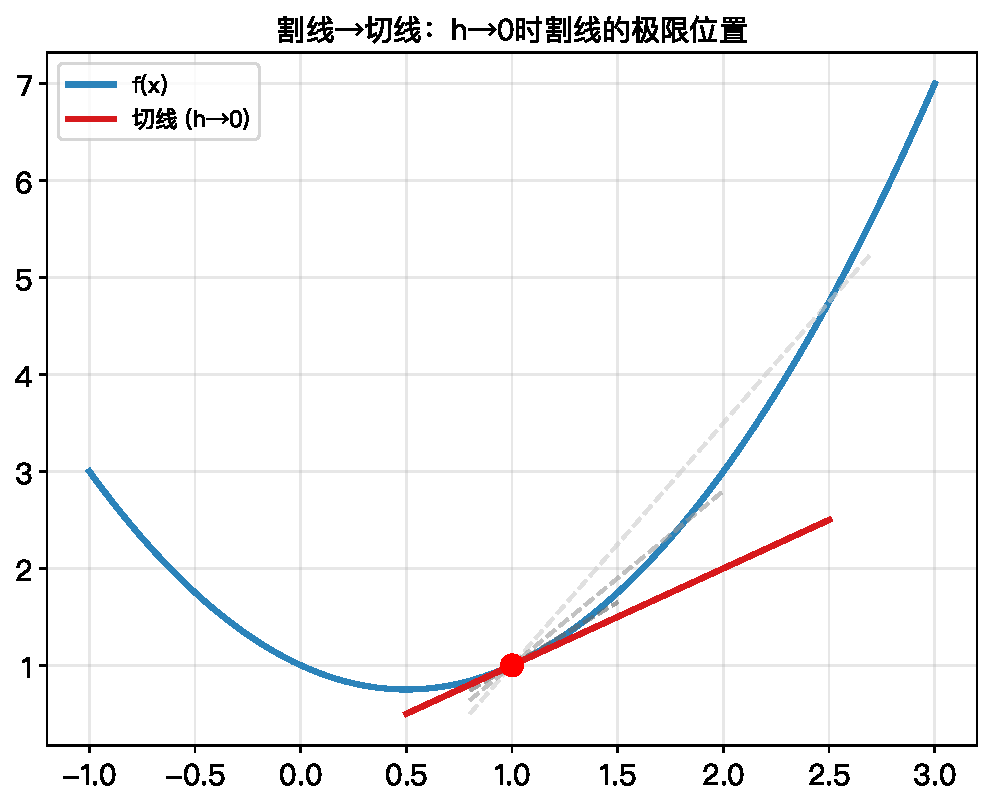
\includegraphics[width=0.7\textwidth]{figures/ch17_tangent.pdf}
\end{center}

割线的斜率：\(\frac{f(a+h)-f(a)}{h}\)\\
当 \(h \to 0\) 时，割线趋近于切线，斜率趋近于导数。
\end{examplebox}

\begin{examplebox}[2——切线斜率 = 导数]
\begin{center}
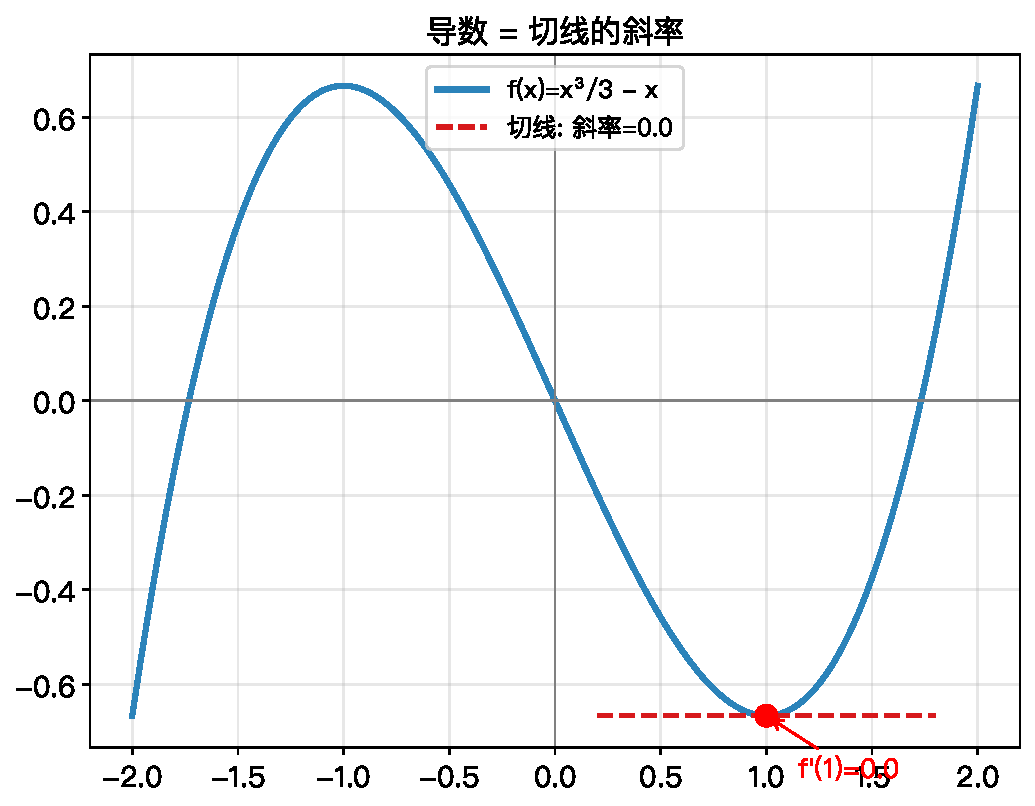
\includegraphics[width=0.7\textwidth]{figures/ch17_derivative_slope.pdf}
\end{center}

\(f(x) = \frac{x^3}{3} - x\)，在 \(x=1\) 处导数 \(f'(1)=0\)——切线水平。
\end{examplebox}


% ============================================================
\section{基本求导公式}
% ============================================================

\begin{theorembox}[基本导数公式]
\begin{align*}
\frac{d}{dx}(c) &= 0 &\text{（常数导数为0）}\\
\frac{d}{dx}(x^n) &= nx^{n-1} &\text{（幂函数）}\\
\frac{d}{dx}(\sin x) &= \cos x \\
\frac{d}{dx}(\cos x) &= -\sin x \\
\frac{d}{dx}(e^x) &= e^x &\text{（最重要的导数！）}\\
\frac{d}{dx}(\ln x) &= \frac{1}{x}
\end{align*}
\end{theorembox}

\begin{examplebox}[3——用定义求导数]
用定义求 \(f(x)=x^2\) 在 \(x=3\) 处的导数：
\[
f'(3) = \lim_{h\to0} \frac{(3+h)^2 - 9}{h}
= \lim_{h\to0} \frac{9 + 6h + h^2 - 9}{h}
= \lim_{h\to0} (6 + h) = 6
\]

由公式：\(f'(x)=2x\)，所以 \(f'(3)=6\)——一致。
\end{examplebox}


% ============================================================
\section{本章小结}
% ============================================================

\begin{progressbox}
\textbf{导数}：\(f'(a) = \lim_{h\to0} \frac{f(a+h)-f(a)}{h}\)

\textbf{几何意义}：切线的斜率

\textbf{基本公式}：\((x^n)'=nx^{n-1}\)，\((\sin x)'=\cos x\)，\((e^x)'=e^x\)，\((\ln x)'=1/x\)

\(e^x\) 的导数等于自己——这是 \(e\) 最重要的性质
\end{progressbox}

% ============================================================
% 习题
% ============================================================
\section{习题}

\begin{exercise}[0]
导数 \(f'(a)\) 的极限定义是什么？
\end{exercise}
\begin{exercise}[0]
导数的几何意义是什么？
\end{exercise}
\begin{exercise}[0]
常数函数的导数是多少？
\end{exercise}
\begin{exercise}[0]
\(e^x\) 的导数是什么？
\end{exercise}

\begin{exercise}[1]
用定义求 \(f(x)=x\) 在 \(x=2\) 处的导数。
\end{exercise}
\begin{exercise}[1]
用定义求 \(f(x)=3\) 的导数。
\end{exercise}
\begin{exercise}[1]
用公式求 \(f(x)=x^5\) 的导数。
\end{exercise}
\begin{exercise}[1]
求 \(f(x)=x^2\) 在 \(x=-1\) 处的导数值。
\end{exercise}

\begin{exercise}[2]
用定义求 \(f(x)=x^3\) 在 \(x=1\) 处的导数。
\end{exercise}
\begin{exercise}[2]
求曲线 \(y=x^2\) 在点 \((2,4)\) 处的切线方程。
\end{exercise}
\begin{exercise}[2]
求 \(f(x)=\sin x\) 在 \(x=0\) 处的导数。
\end{exercise}
\begin{exercise}[2]
求 \(f(x)=\frac{1}{x}\) 在 \(x=2\) 处的导数。
\end{exercise}

\begin{exercise}[3]
用定义求 \(f(x)=\sqrt{x}\) 在 \(x=4\) 处的导数。
\end{exercise}
\begin{exercise}[3]
求曲线 \(y=x^3\) 在 \(x=1\) 处的切线方程。
\end{exercise}
\begin{exercise}[3]
已知 \(f'(2)=5\)，用定义写出极限 \(\lim_{h\to0} \frac{f(2+h)-f(2)}{h}\) 的值。
\end{exercise}
\begin{exercise}[3]
求 \(f(x)=x^4\) 在 \(x=-2\) 处的导数值和切线方程。
\end{exercise}
\begin{exercise}[3]
证明 \((x^2)' = 2x\) 用定义。
\end{exercise}

\begin{exercise}[4]
用定义证明 \((x^n)' = nx^{n-1}\) 对 \(n=3\) 成立。
\end{exercise}
\begin{exercise}[4]
求曲线 \(y=e^x\) 在 \(x=0\) 处的切线方程。
\end{exercise}
\begin{exercise}[4]
求 \(f(x)=\cos x\) 在 \(x=0\) 处的导数。
\end{exercise}
\begin{exercise}[4]
已知 \(f(x)=x^3-2x+1\)，求 \(f'(1)\) 和 \(x=1\) 处的切线方程。
\end{exercise}
\begin{exercise}[4]
证明：若 \(f\) 在 \(x=a\) 处可导，则 \(f\) 在 \(x=a\) 处连续。
\end{exercise}

\begin{exercise}[5]
用定义证明 \((\sin x)' = \cos x\)。
\end{exercise}
\begin{exercise}[5]
求 \(f(x)=\ln x\) 在 \(x=1\) 处的导数。
\end{exercise}
\begin{exercise}[5]
求曲线 \(y=\frac{1}{x}\) 在点 \((1,1)\) 处的切线方程和法线方程。
\end{exercise}
\begin{exercise}[5]
已知 \(\lim_{h\to0} \frac{f(1+h)-f(1)}{h} = 4\)，求 \(f'(1)\)。
\end{exercise}

\begin{exercise}[6]
用定义求 \(f(x)=|x|\) 在 \(x=0\) 处的左右导数，它可导吗？
\end{exercise}
\begin{exercise}[6]
求曲线 \(y=\sqrt{x}\) 上切线斜率为 \(\frac{1}{4}\) 的点。
\end{exercise}
\begin{exercise}[6]
证明：若 \(f\) 是偶函数且可导，则 \(f'\) 是奇函数。
\end{exercise}

\begin{exercise}[7]
用定义求 \(f(x)=\sin x\) 的导数公式，并求出 \(f(x)\) 在 \(x=\frac{\pi}{3}\) 处的切线方程。
\end{exercise}


% ch18: 求导法则
\chapter{求导法则——四则运算与链式法则}
\begin{applicationbox}
学完本章：掌握四则运算法则、链式法则、隐函数求导
\end{applicationbox}

\section{四则运算法则}
\[(f\pm g)'=f'\pm g',\quad (fg)'=f'g+fg',\quad \left(\frac{f}{g}\right)'=\frac{f'g-fg'}{g^2}\]

\textbf{乘法法则的 ε-δ 证明：}
\[
(fg)'(a)=\lim_{h\to0}\frac{f(a+h)g(a+h)-f(a)g(a)}{h}
\]
\[
=\lim_{h\to0}\frac{[f(a+h)-f(a)]g(a+h)+f(a)[g(a+h)-g(a)]}{h}
\]
\[
=\lim_{h\to0}\frac{f(a+h)-f(a)}{h}\cdot g(a+h) + f(a)\cdot\frac{g(a+h)-g(a)}{h}
\]
由 \(g\) 连续（可导⇒连续）知 \(\lim g(a+h)=g(a)\)，故 \((fg)'(a)=f'(a)g(a)+f(a)g'(a)\)。\(\blacksquare\)

\section{链式法则}
\[(f(g(x)))' = f'(g(x))\cdot g'(x)\]

\textbf{ε-δ 证明：} 设 \(u=g(x)\)，\(y=f(u)\)。
\[
\frac{dy}{dx}=\lim_{h\to0}\frac{f(g(x+h))-f(g(x))}{h}
=\lim_{h\to0}\frac{f(g(x+h))-f(g(x))}{g(x+h)-g(x)}\cdot\frac{g(x+h)-g(x)}{h}
\]
令 \(k=g(x+h)-g(x)\)，当 \(h\to0\) 时 \(k\to0\)（由 \(g\) 连续），故
\[
\frac{dy}{dx}=\lim_{k\to0}\frac{f(u+k)-f(u)}{k}\cdot\lim_{h\to0}\frac{g(x+h)-g(x)}{h}=f'(u)g'(x)
\]
其中第一个极限存在是因为 \(f\) 可导，第二个因为 \(g\) 可导。\(\blacksquare\)

\section{隐函数求导}
\begin{examplebox}[3]
\(x^2+y^2=1\)，两边对 \(x\) 求导：\(2x+2yy'=0\)，\(y'=-\frac{x}{y}\)
\end{examplebox}

\section{习题}
\begin{exercise}[0] \((x^2)'=?\) \end{exercise}
\begin{exercise}[0] \((\sin x)'=?\) \end{exercise}
\begin{exercise}[0] 链式法则的公式是什么？\end{exercise}
\begin{exercise}[0] \((e^x)'=?\) \end{exercise}
\begin{exercise}[1] 求 \(f(x)=3x^2+2x-1\) 的导数。\end{exercise}
\begin{exercise}[1] 求 \(f(x)=x\sin x\) 的导数。\end{exercise}
\begin{exercise}[1] 求 \(f(x)=\frac{x}{x+1}\) 的导数。\end{exercise}
\begin{exercise}[1] 求 \(f(x)=\sin(2x)\) 的导数。\end{exercise}
\begin{exercise}[2] 求 \(f(x)=x^2\cos x\) 的导数。\end{exercise}
\begin{exercise}[2] 求 \(f(x)=\ln(x^2+1)\) 的导数。\end{exercise}
\begin{exercise}[2] 求 \(f(x)=e^{3x}\) 的导数。\end{exercise}
\begin{exercise}[2] 曲线 \(x^2+xy+y^2=3\) 在点 \((1,1)\) 处的切线斜率。\end{exercise}
\begin{exercise}[3] 求 \(f(x)=\tan x\) 的导数。\end{exercise}
\begin{exercise}[3] 求 \(f(x)=\sin^2 x + \cos^2 x\) 的导数（先化简再求）。\end{exercise}
\begin{exercise}[3] 求 \(y=\ln(\sin x)\) 的导数。\end{exercise}
\begin{exercise}[3] 求 \(f(x)=\frac{e^x}{x}\) 的导数。\end{exercise}
\begin{exercise}[3] \(xy=e^{x+y}\) 求 \(y'\)。\end{exercise}
\begin{exercise}[4] 求 \(f(x)=\sqrt{1+x^2}\) 的导数。\end{exercise}
\begin{exercise}[4] 求 \(f(x)=\sin(e^x)\) 的导数。\end{exercise}
\begin{exercise}[4] 求 \(y=\arctan x\) 的导数。\end{exercise}
\begin{exercise}[4] 求 \(f(x)=x^x\) 的导数（提示：取对数）。\end{exercise}
\begin{exercise}[4] \(y^2 = x^2 + xy\) 求 \(y'\)。\end{exercise}
\begin{exercise}[5] 求 \(f(x)=e^{\sin x}\cos x\) 的导数。\end{exercise}
\begin{exercise}[5] 求 \(y=\arcsin x\) 的导数。\end{exercise}
\begin{exercise}[5] 求 \(f(x)=\ln(x+\sqrt{1+x^2})\) 的导数。\end{exercise}
\begin{exercise}[5] 求 \(y=x^{\sin x}\) 的导数。\end{exercise}
\begin{exercise}[6] 证明 \((\sec x)'=\sec x\tan x\)。\end{exercise}
\begin{exercise}[6] 求 \(f(x)=\sin(\cos(\tan x))\) 的导数。\end{exercise}
\begin{exercise}[6] 求曲线 \(x^3+y^3=3xy\) 在 \((\frac32,\frac32)\) 处的切线。\end{exercise}
\begin{exercise}[7] 用链式法则证明若 \(f\) 是奇函数且可导，则 \(f'\) 是偶函数。\end{exercise}

% ch19: 微分中值定理
\chapter{微分中值定理——罗尔、拉格朗日、柯西}
\begin{applicationbox}
学完本章：掌握三个中值定理及其关系，会用中值定理证明不等式
\end{applicationbox}

\section{罗尔定理}
若 \(f\) 在 \([a,b]\) 连续、\((a,b)\) 可导、且 \(f(a)=f(b)\)，则存在 \(c\in(a,b)\) 使 \(f'(c)=0\)。

\textbf{ε-δ 证明：} 若 \(f\) 在 \([a,b]\) 上恒为常数，则任意 \(c\) 处 \(f'(c)=0\)，结论成立。
否则 \(f\) 在内部某点取到最大值或最小值（由闭区间上连续函数的最值定理）。
设 \(c\) 为极值点，不妨设是最大值点。取 \(h\) 充分小使 \(c+h\in(a,b)\)，
则 \(f(c+h)\le f(c)\)。当 \(h>0\) 时 \(\frac{f(c+h)-f(c)}{h}\le0\)；
当 \(h<0\) 时 \(\frac{f(c+h)-f(c)}{h}\ge0\)。
令 \(h\to0\) 取极限，由导数存在得 \(f'(c)=\lim_{h\to0^+}\le0\) 且 \(f'(c)=\lim_{h\to0^-}\ge0\)，
故 \(f'(c)=0\)。\quad\(\blacksquare\)

\section{拉格朗日中值定理}
若 \(f\) 在 \([a,b]\) 连续、\((a,b)\) 可导，则存在 \(c\in(a,b)\) 使：
\[f'(c) = \frac{f(b)-f(a)}{b-a}\]

\textbf{ε-δ 证明：} 构造辅助函数
\[
g(x)=f(x)-\frac{f(b)-f(a)}{b-a}(x-a)
\]
则 \(g(a)=f(a)\)，\(g(b)=f(b)-\frac{f(b)-f(a)}{b-a}(b-a)=f(a)\)，即 \(g(a)=g(b)\)。
由罗尔定理，存在 \(c\in(a,b)\) 使 \(g'(c)=0\)。
而 \(g'(x)=f'(x)-\frac{f(b)-f(a)}{b-a}\)，故 \(f'(c)=\frac{f(b)-f(a)}{b-a}\)。\(\blacksquare\)

\begin{center}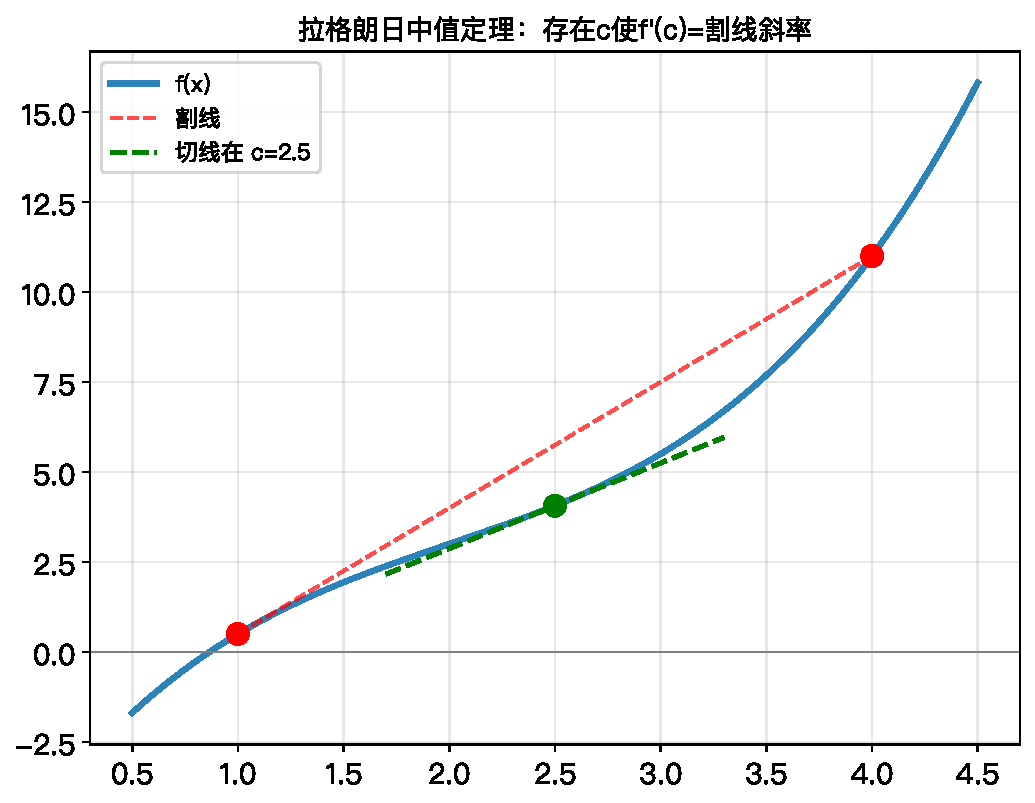
\includegraphics[width=0.6\textwidth]{figures/ch19_mvt.pdf}\end{center}

\begin{examplebox}[1]
证明 \(|\sin b - \sin a| \le |b-a|\)。由中值定理，\(\sin b-\sin a = \cos c \cdot (b-a)\)，\(|\cos c|\le1\)。
\end{examplebox}

\section{柯西中值定理}
若 \(f,g\) 在 \([a,b]\) 连续、\((a,b)\) 可导且 \(g'(x)\neq0\)，则存在 \(c\in(a,b)\) 使：
\[\frac{f(b)-f(a)}{g(b)-g(a)} = \frac{f'(c)}{g'(c)}\]

\section{习题}
\begin{exercise}[0] 罗尔定理要求 \(f(a)\) 和 \(f(b)\) 有什么关系？\end{exercise}
\begin{exercise}[0] 拉格朗日中值定理的几何意义是什么？\end{exercise}
\begin{exercise}[0] 中值定理中的 \(c\) 在哪个区间内？\end{exercise}
\begin{exercise}[0] 若 \(f'(x)=0\) 恒成立，\(f(x)\) 是什么函数？\end{exercise}
\begin{exercise}[1] 验证 \(f(x)=x^2-4x+3\) 在 \([1,3]\) 上满足罗尔定理条件，求 \(c\)。\end{exercise}
\begin{exercise}[1] 对 \(f(x)=x^2\) 在 \([1,3]\) 上应用中值定理求 \(c\)。\end{exercise}
\begin{exercise}[1] 证明 \(\sqrt{1+h} < 1 + h/2\)（\(h>0\)）。\end{exercise}
\begin{exercise}[1] 若 \(f'(x)=2\)，且 \(f(1)=3\)，求 \(f(x)\)。\end{exercise}
\begin{exercise}[2] 验证 \(f(x)=x^3-3x\) 在 \([-\sqrt{3},\sqrt{3}]\) 上满足罗尔定理。\end{exercise}
\begin{exercise}[2] 证明 \(|\arctan b - \arctan a| \le |b-a|\)。\end{exercise}
\begin{exercise}[2] 用中值定理证明 \(e^x > 1+x\)（\(x>0\)）。\end{exercise}
\begin{exercise}[2] 若 \(f'(x)=3x^2\)，\(f(0)=1\)，求 \(f(x)\)。\end{exercise}
\begin{exercise}[3] 证明 \(\frac{b-a}{b} < \ln\frac{b}{a} < \frac{b-a}{a}\)（\(0<a<b\)）。\end{exercise}
\begin{exercise}[3] 证明 \(|\sin x - \sin y| \le |x-y|\)。\end{exercise}
\begin{exercise}[3] 用中值定理证明 \(\ln(1+x) < x\)（\(x>0\)）。\end{exercise}
\begin{exercise}[3] 若 \(f'(x)=g'(x)\) 对所有 \(x\) 成立，证明 \(f(x)=g(x)+C\)。\end{exercise}
\begin{exercise}[3] 证明 \(x > \sin x > x - x^3/6\)（\(x>0\)）。\end{exercise}
\begin{exercise}[4] 若 \(f''(x)>0\)，证明 \(f\) 是凸函数。\end{exercise}
\begin{exercise}[4] 证明方程 \(x^3-3x+1=0\) 在 \((0,1)\) 内至多有一个根。\end{exercise}
\begin{exercise}[4] 用中值定理证明 \(\sqrt{1+x} < 1 + x/2\)（\(x>0\)）。\end{exercise}
\begin{exercise}[4] 证明若 \(f'(x)=f(x)\)，则 \(f(x)=Ce^x\)。\end{exercise}
\begin{exercise}[4] 证明 \(\lim_{x\to0} \frac{\sin x}{x}=1\) 用中值定理。\end{exercise}
\begin{exercise}[5] 证明 \(\frac{x}{1+x^2} < \arctan x < x\)（\(x>0\)）。\end{exercise}
\begin{exercise}[5] 若 \(f\) 在 \([0,1]\) 可导，\(f(0)=0\)，\(f(1)=1\)，证明存在 \(c\) 使 \(f'(c)=1\)。\end{exercise}
\begin{exercise}[5] 证明：若 \(f'(x)\) 有界，则 \(f\) 一致连续。\end{exercise}
\begin{exercise}[5] \(f\) 在 \([0,1]\) 可导，\(f(0)=0\)，\(f(1)=1\)，证明存在不同 \(a,b\) 使 \(1/f'(a)+1/f'(b)=2\)。\end{exercise}
\begin{exercise}[6] 证明达布定理：导函数具有介值性。\end{exercise}
\begin{exercise}[6] 若 \(f\) 在 \([a,b]\) 可导且 \(f'(a)<k<f'(b)\)，证明存在 \(c\) 使 \(f'(c)=k\)。\end{exercise}
\begin{exercise}[6] 证明：若 \(f\) 在 \(\mathbb{R}\) 上可导且 \(|f'(x)|\le M\)，则 \(f\) 一致连续。\end{exercise}
\begin{exercise}[7] 设 \(f\) 在 \([0,1]\) 可导，\(f(0)=0\)，\(f(1)=1\)，\(f'(x)\neq0\)，证明存在 \(c,d\) 使 \(1/f'(c)+1/f'(d)=2\)。\end{exercise}

% ch20: 泰勒公式与洛必达法则
\chapter{泰勒公式与洛必达法则}
\begin{applicationbox}
学完本章：用多项式逼近函数、用导数求极限
\end{applicationbox}

\section{洛必达法则}
若 \(\lim\frac{f(x)}{g(x)}\) 是 \(\frac00\) 或 \(\frac\infty\infty\) 型，且 \(\lim\frac{f'(x)}{g'(x)}\) 存在，则：
\[\lim\frac{f(x)}{g(x)} = \lim\frac{f'(x)}{g'(x)}\]

\textbf{ε-δ 证明（\(\frac00\) 型）：} 设 \(f(a)=g(a)=0\)，\(\lim_{x\to a}\frac{f'(x)}{g'(x)}=L\)。
对任意 \(\varepsilon>0\)，存在 \(\delta>0\) 使 \(0<|x-a|<\delta\) 时 \(|\frac{f'(x)}{g'(x)}-L|<\varepsilon\)。
对 \(x\in(a,a+\delta)\)，由柯西中值定理，存在 \(c\in(a,x)\) 使
\(\frac{f(x)-f(a)}{g(x)-g(a)}=\frac{f(x)}{g(x)}=\frac{f'(c)}{g'(c)}\)，
故 \(|\frac{f(x)}{g(x)}-L|=|\frac{f'(c)}{g'(c)}-L|<\varepsilon\)。\(\blacksquare\)

\begin{examplebox}[1]
\(\lim_{x\to0}\frac{\sin x}{x} = \lim_{x\to0}\frac{\cos x}{1} = 1\)
\end{examplebox}

\section{泰勒公式}
\(f(x) = f(a) + f'(a)(x-a) + \frac{f''(a)}{2!}(x-a)^2 + \cdots + \frac{f^{(n)}(a)}{n!}(x-a)^n + R_n(x)\)

\textbf{拉格朗日余项（ε-δ 证明框架）：} 令 \(F(t)=f(t)+\sum_{k=1}^{n-1}\frac{f^{(k)}(t)}{k!}(x-t)^k\)，
\(G(t)=(x-t)^n\)。由柯西中值定理，存在 \(\xi\) 在 \(a\) 与 \(x\) 之间使
\[R_n(x)=\frac{f^{(n)}(\xi)}{n!}(x-a)^n\]
即余项可表示为高阶导数在中间点的值乘以幂次——这是泰勒定理的精确形式。

\begin{examplebox}[2——常用展开]
\[e^x=1+x+\frac{x^2}{2!}+\frac{x^3}{3!}+\cdots,\quad \sin x = x-\frac{x^3}{3!}+\frac{x^5}{5!}-\cdots\]
\end{examplebox}

\section{习题}
\begin{exercise}[0] 洛必达法则适用于哪两种不定式？\end{exercise}
\begin{exercise}[0] \(\lim_{x\to0}\frac{\sin x}{x}\) 用洛必达怎么算？\end{exercise}
\begin{exercise}[0] \(e^x\) 在 \(x=0\) 处的泰勒展开第一项是什么？\end{exercise}
\begin{exercise}[0] \(\sin x\) 的泰勒展开的第一项是什么？\end{exercise}
\begin{exercise}[1] 求 \(\lim_{x\to0}\frac{e^x-1}{x}\)。\end{exercise}
\begin{exercise}[1] 求 \(\lim_{x\to0}\frac{\ln(1+x)}{x}\)。\end{exercise}
\begin{exercise}[1] 求 \(\lim_{x\to1}\frac{\ln x}{x-1}\)。\end{exercise}
\begin{exercise}[1] 写出 \(e^x\) 在 \(x=0\) 处的3次泰勒多项式。\end{exercise}
\begin{exercise}[2] 求 \(\lim_{x\to0}\frac{1-\cos x}{x^2}\)。\end{exercise}
\begin{exercise}[2] 求 \(\lim_{x\to\infty}\frac{x}{e^x}\)。\end{exercise}
\begin{exercise}[2] 求 \(\lim_{x\to0}\frac{\tan x}{x}\)。\end{exercise}
\begin{exercise}[2] 写出 \(\sin x\) 在 \(x=0\) 处的3次泰勒多项式。\end{exercise}
\begin{exercise}[3] 求 \(\lim_{x\to0}\frac{x-\sin x}{x^3}\)。\end{exercise}
\begin{exercise}[3] 求 \(\lim_{x\to0^+} x\ln x\)。\end{exercise}
\begin{exercise}[3] 求 \(\lim_{x\to\infty}\frac{\ln x}{x}\)。\end{exercise}
\begin{exercise}[3] 写出 \(\cos x\) 在 \(x=0\) 处的4次泰勒多项式。\end{exercise}
\begin{exercise}[3] 用泰勒展开求 \(e^{0.1}\) 的近似值（精确到0.001）。\end{exercise}
\begin{exercise}[4] 求 \(\lim_{x\to0}\frac{e^x-1-x}{x^2}\)。\end{exercise}
\begin{exercise}[4] 求 \(\lim_{x\to0}\frac{\arctan x - x}{x^3}\)。\end{exercise}
\begin{exercise}[4] 求 \(\lim_{x\to0}\left(\frac{1}{x} - \frac{1}{e^x-1}\right)\)。\end{exercise}
\begin{exercise}[4] 写出 \(\ln(1+x)\) 在 \(x=0\) 处的3次泰勒多项式。\end{exercise}
\begin{exercise}[4] 用二次泰勒展开近似 \(\sqrt{1.1}\)。\end{exercise}
\begin{exercise}[5] 求 \(\lim_{x\to0}\frac{\sin x - x + x^3/6}{x^5}\)。\end{exercise}
\begin{exercise}[5] 求 \(\lim_{x\to\infty}\left(1+\frac{1}{x}\right)^x\) 用洛必达法则。\end{exercise}
\begin{exercise}[5] 证明 \(\lim_{x\to0}\frac{x-\sin x}{x^3}=\frac16\)。\end{exercise}
\begin{exercise}[5] 用3次泰勒展开近似 \(\sin(0.1)\) 并估计误差。\end{exercise}
\begin{exercise}[6] 求 \(\lim_{x\to0^+} x^x\)。\end{exercise}
\begin{exercise}[6] 写出 \(\arctan x\) 在 \(x=0\) 处的5次泰勒展开。\end{exercise}
\begin{exercise}[6] 证明 \(e^x > 1 + x + x^2/2\)（\(x>0\)）。\end{exercise}
\begin{exercise}[7] 用泰勒展开证明 \(\sin x > x - x^3/6\)（\(x>0\)）。\end{exercise}

% ch21: 导数的应用
\chapter{导数的应用——极值、凹凸、作图}
\begin{applicationbox}
学完本章：用导数分析函数——找极值、判断凹凸、完整作图
\end{applicationbox}

\section{极值}
\(f'(x)=0\) 的点叫\textbf{驻点}。若 \(f'\) 由正变负则为极大值，由负变正则为极小值。

\textbf{费马定理的 ε-δ 证明：} 设 \(f\) 在 \(x=c\) 处取局部极大值，则存在 \(\delta>0\) 使 \(|x-c|<\delta\) 时 \(f(x)\le f(c)\)。
对 \(h\in(0,\delta)\)，\(\frac{f(c+h)-f(c)}{h}\le0\)，取极限得 \(f'(c)\le0\)。
对 \(h\in(-\delta,0)\)，\(\frac{f(c+h)-f(c)}{h}\ge0\)，取极限得 \(f'(c)\ge0\)。
故 \(f'(c)=0\)。\(\blacksquare\)

\textbf{单调性的 ε-δ 判别：} 若 \(f'(x)>0\) 恒成立，则由拉格朗日中值定理，
对任意 \(x_1<x_2\)，存在 \(c\in(x_1,x_2)\) 使 \(f(x_2)-f(x_1)=f'(c)(x_2-x_1)>0\)，故 \(f\) 严格递增。\(\blacksquare\)

\begin{center}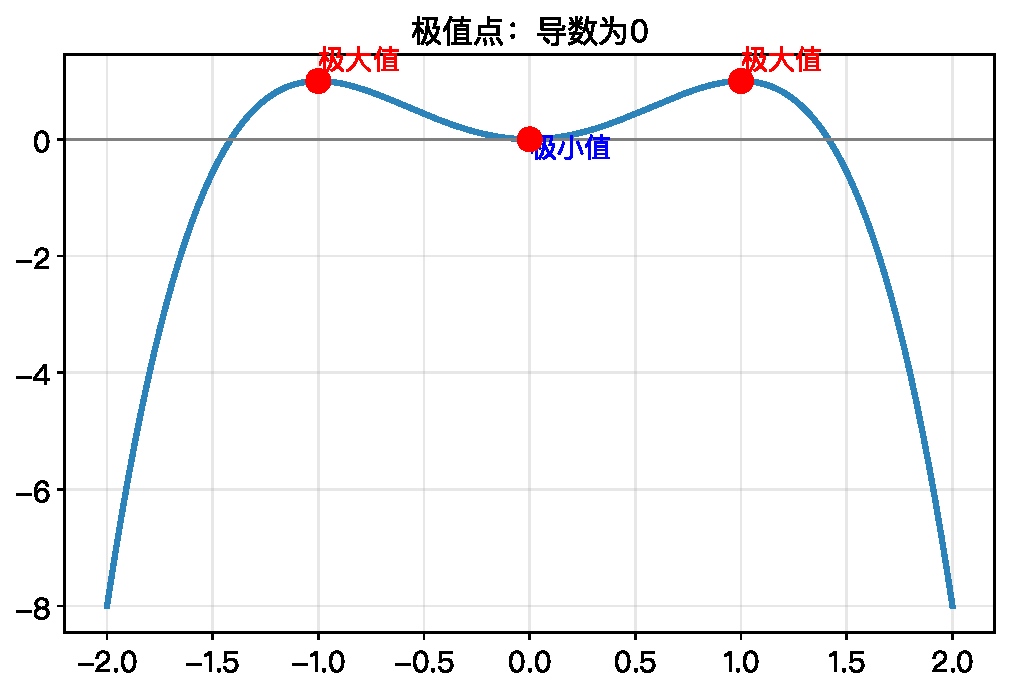
\includegraphics[width=0.6\textwidth]{figures/ch21_extrema.pdf}\end{center}

\section{凹凸性与拐点}
\(f''(x)>0\) 为凹（开口向上），\(f''(x)<0\) 为凸（开口向下）。\(f''(x)=0\) 且变号处为\textbf{拐点}。

\begin{center}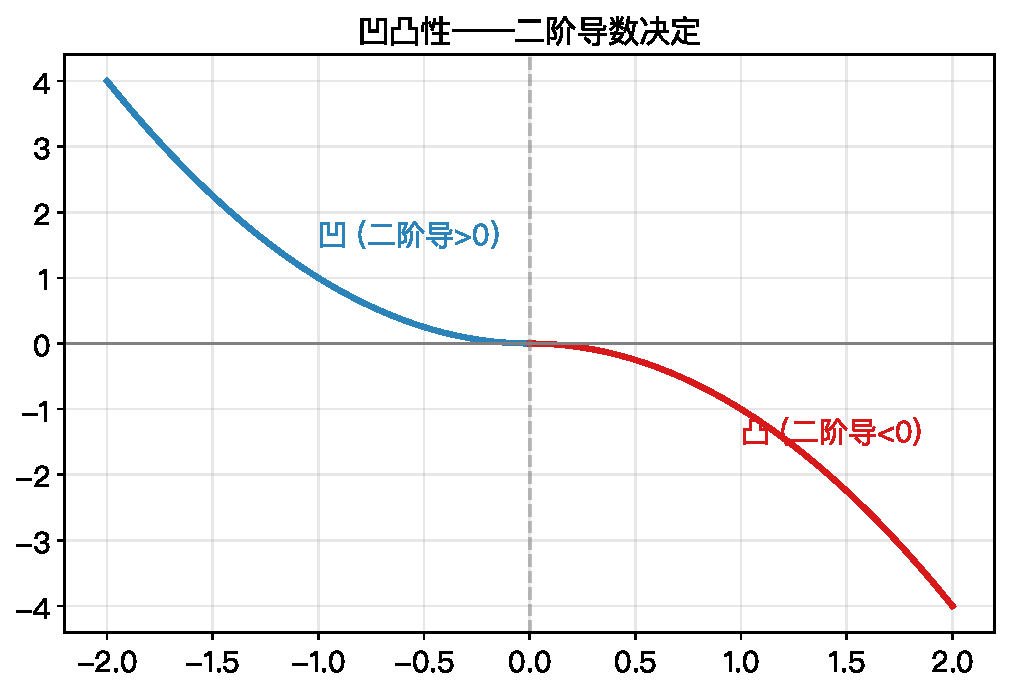
\includegraphics[width=0.6\textwidth]{figures/ch21_concavity.pdf}\end{center}

\section{函数作图的完整流程}
\begin{enumerate}
\item 确定定义域、对称性
\item 求 \(f'(x)\) 找驻点和单调区间
\item 求 \(f''(x)\) 找拐点和凹凸区间
\item 求渐近线
\item 列表、描点、连线
\end{enumerate}

\section{习题}
\begin{exercise}[0] \(f'(x)=0\) 的点叫什么？\end{exercise}
\begin{exercise}[0] \(f''(x)>0\) 表示函数是凹还是凸？\end{exercise}
\begin{exercise}[0] 极大值点的导数一定为0吗？\end{exercise}
\begin{exercise}[0] 拐点处 \(f''(x)\) 等于多少？\end{exercise}
\begin{exercise}[1] 求 \(f(x)=x^2-4x+3\) 的极值。\end{exercise}
\begin{exercise}[1] 判断 \(f(x)=x^3\) 在 \(x=0\) 处是否有极值。\end{exercise}
\begin{exercise}[1] 求 \(f(x)=x^3-3x\) 的极值点。\end{exercise}
\begin{exercise}[1] 求 \(f(x)=x^2\) 的凹凸性。\end{exercise}
\begin{exercise}[2] 求 \(f(x)=2x^3-3x^2-12x+1\) 的极值。\end{exercise}
\begin{exercise}[2] 求 \(f(x)=x^3-6x^2\) 的凹凸区间和拐点。\end{exercise}
\begin{exercise}[2] 求 \(f(x)=x+\frac{1}{x}\) 的极值。\end{exercise}
\begin{exercise}[2] 求证 \(e^x \ge x+1\)。\end{exercise}
\begin{exercise}[3] 求 \(f(x)=x^4-4x^3\) 的极值和拐点。\end{exercise}
\begin{exercise}[3] 求 \(f(x)=x\ln x\) 的极值。\end{exercise}
\begin{exercise}[3] 求 \(f(x)=\frac{x^2}{1+x^2}\) 的渐近线。\end{exercise}
\begin{exercise}[3] 求内接于圆的最大矩形面积。\end{exercise}
\begin{exercise}[3] 做一个容积为 \(V\) 的无盖圆柱形水桶，求最小表面积。\end{exercise}
\begin{exercise}[4] 求 \(f(x)=x^2e^{-x}\) 的极值和拐点。\end{exercise}
\begin{exercise}[4] 求 \(f(x)=\ln(1+x^2)\) 的凹凸区间。\end{exercise}
\begin{exercise}[4] 求 \(f(x)=\frac{x}{x^2-1}\) 的渐近线。\end{exercise}
\begin{exercise}[4] 围栏长100米，靠墙围最大矩形面积。\end{exercise}
\begin{exercise}[4] 证明 \(x^3-3x+1=0\) 在 \((0,1)\) 内恰有一个根。\end{exercise}
\begin{exercise}[5] 求 \(f(x)=e^{-x^2}\) 的极值、凹凸、拐点。\end{exercise}
\begin{exercise}[5] 作 \(f(x)=\frac{x}{1-x^2}\) 的完整图像。\end{exercise}
\begin{exercise}[5] 求 \(f(x)=x-\arctan x\) 的凹凸区间。\end{exercise}
\begin{exercise}[5] 证明 \(\ln(1+x) \le x\)（\(x>-1\)）。\end{exercise}
\begin{exercise}[6] 作 \(f(x)=x^{1/x}\)（\(x>0\)）的图像。\end{exercise}
\begin{exercise}[6] 求 \(f(x)=\frac{e^x}{x}\) 的完整图像分析。\end{exercise}
\begin{exercise}[6] 证明 \(x^\alpha \le \alpha x + (1-\alpha)\)（\(x>0, 0<\alpha<1\)）。\end{exercise}
\begin{exercise}[7] 求 \(f(x)=\frac{x^3}{(x-1)^2}\) 的完整图像分析（含渐近线）。\end{exercise}

% 第三编结束，进入第四编

% ============================================================
% 第四编：黎曼积分
\part{黎曼积分——累积的度量}
% ch22: 定积分概念
\chapter{定积分的概念——从面积到黎曼和}
\begin{applicationbox}
学完本章：理解黎曼和与定积分定义，掌握几何意义
\end{applicationbox}

\section{面积问题} 求曲线下的面积——用矩形逼近：\(\sum f(x_i^*)\Delta x_i\)，当分割无限细时取极限。

\section{定积分定义} \(\int_a^b f(x)dx = \lim_{\max\Delta x_i\to0}\sum_{i=1}^n f(\xi_i)\Delta x_i\)

\textbf{用 ε-δ 语言：} 对任意 \(\varepsilon>0\)，存在 \(\delta>0\)，
使得当分割的最大宽度 \(\|\Delta\|<\delta\) 时，对任意取点方式 \(\xi_i\)，
\[
\left|\sum_{i=1}^n f(\xi_i)\Delta x_i - \int_a^b f(x)dx\right| < \varepsilon
\]

\section{连续函数必可积（ε-δ 证明）}
设 \(f\) 在 \([a,b]\) 上连续，则 \(f\) 一致连续：
对任意 \(\varepsilon>0\)，存在 \(\delta>0\)，使 \(|x-y|<\delta\) 时 \(|f(x)-f(y)|<\frac{\varepsilon}{b-a}\)。
取分割 \(a=x_0<x_1<\cdots<x_n=b\) 满足最大宽度 \(<\delta\)。记
\(M_i=\max_{[x_{i-1},x_i]}f\)，\(m_i=\min_{[x_{i-1},x_i]}f\)，则
\[
U-L = \sum (M_i-m_i)\Delta x_i < \frac{\varepsilon}{b-a}\sum\Delta x_i = \varepsilon
\]
由达布定理，\(f\) 在 \([a,b]\) 上黎曼可积。\(\blacksquare\)

\section{几何意义} \(\int_a^b f(x)dx\) = 曲线与 \(x\) 轴围成的面积（若 \(f\ge0\)）

\begin{examplebox}[1——黎曼和近似]
\(\int_0^1 x^2 dx\) 用 \(n=4\) 个右端点矩形：\(\frac14[(0.25)^2+(0.5)^2+(0.75)^2+1^2]=0.46875\)，精确值 \(1/3\approx0.333\)。
\end{examplebox}

\section{习题}
\begin{exercise}[0] 定积分 \(\int_a^b f(x)dx\) 的几何意义是什么？\end{exercise}
\begin{exercise}[0] 黎曼和中 \(\Delta x_i\) 代表什么？\end{exercise}
\begin{exercise}[0] 若 \(f(x)\ge0\)，\(\int_a^b f(x)dx\) 的符号是？\end{exercise}
\begin{exercise}[0] 定积分 \(\int_a^a f(x)dx\) 等于多少？\end{exercise}
\begin{exercise}[1] 用右端点矩形近似 \(\int_0^1 x dx\)（\(n=4\)）。\end{exercise}
\begin{exercise}[1] 用左端点矩形近似 \(\int_0^1 x^2 dx\)（\(n=4\)）。\end{exercise}
\begin{exercise}[1] 求 \(\int_0^2 3 dx\) 的精确值（几何意义）。\end{exercise}
\begin{exercise}[1] 求 \(\int_0^1 x dx\) 的精确值。\end{exercise}
\begin{exercise}[2] 用 \(n=6\) 的黎曼和近似 \(\int_0^\pi \sin x dx\)。\end{exercise}
\begin{exercise}[2] 求 \(\int_0^a x dx\) 的值。\end{exercise}
\begin{exercise}[2] 求 \(\int_{-a}^a x^3 dx\) 的值（利用奇函数性质）。\end{exercise}
\begin{exercise}[2] 用几何意义求 \(\int_{-1}^1 \sqrt{1-x^2} dx\)。\end{exercise}
\begin{exercise}[3] 用定义计算 \(\int_0^1 x dx\)（取等分分割、右端点）。\end{exercise}
\begin{exercise}[3] 用定义计算 \(\int_0^1 x^2 dx\)。\end{exercise}
\begin{exercise}[3] 比较 \(\int_0^1 x dx\) 和 \(\int_0^1 x^2 dx\) 的大小。\end{exercise}
\begin{exercise}[3] 求 \(\int_0^2 |x-1| dx\) 的值。\end{exercise}
\begin{exercise}[3] 用几何意义求 \(\int_{-1}^1 (1-|x|) dx\)。\end{exercise}
\begin{exercise}[4] 用定义计算 \(\int_0^1 x^3 dx\)。\end{exercise}
\begin{exercise}[4] 求 \(\int_0^1 \sqrt{1-x^2} dx\)（几何意义：四分之一圆）。\end{exercise}
\begin{exercise}[4] 求 \(\int_{-2}^2 (x^3+1) dx\)。\end{exercise}
\begin{exercise}[4] 证明 \(\int_a^b f(x)dx = -\int_b^a f(x)dx\)。\end{exercise}
\begin{exercise}[4] 比较 \(\int_0^1 e^x dx\) 和 \(\int_0^1 e^{x^2} dx\) 的大小。\end{exercise}
\begin{exercise}[5] 用定义证明 \(\int_0^1 x^k dx = \frac{1}{k+1}\)。\end{exercise}
\begin{exercise}[5] 求 \(\int_0^{\pi/2} \sin x dx\) 用黎曼和极限。\end{exercise}
\begin{exercise}[5] 证明 Darboux 定理：上和与下和趋于同一极限。\end{exercise}
\begin{exercise}[5] 求 \(\int_{-1}^1 \frac{1}{1+x^2} dx\)（几何意义不容易直接看出，以后会算）。\end{exercise}
\begin{exercise}[6] 证明 Dirichlet 函数在 \([0,1]\) 上不可积。\end{exercise}
\begin{exercise}[6] 若 \(f\) 在 \([a,b]\) 上连续，证明 \(f\) 可积。\end{exercise}
\begin{exercise}[6] 证明 \(\int_0^1 \frac{\sin x}{x} dx\) 收敛。\end{exercise}
\begin{exercise}[7] 证明：若 \(f\) 在 \([0,1]\) 上可积，则 \(\lim_{n\to\infty}\frac1n\sum_{k=1}^n f(\frac{k}{n}) = \int_0^1 f(x)dx\)。\end{exercise}

% ch23: 微积分基本定理
\chapter{微积分基本定理——牛顿-莱布尼茨公式}
\begin{applicationbox}
学完本章：掌握积分上限函数、微积分基本定理（N-L公式）
\end{applicationbox}

\section{积分上限函数} \(\Phi(x)=\int_a^x f(t)dt\)，则 \(\Phi'(x)=f(x)\)。

\textbf{ε-δ 证明：} 对任意 \(x\)，取 \(h\neq0\) 使 \(x+h\in(a,b)\)。
\[
\frac{\Phi(x+h)-\Phi(x)}{h} = \frac1h\int_x^{x+h} f(t)dt
\]
由积分中值定理，存在 \(\xi\) 在 \(x\) 与 \(x+h\) 之间使上式 \(=f(\xi)\)。
由于 \(f\) 连续，对任意 \(\varepsilon>0\)，存在 \(\delta>0\) 使 \(|t-x|<\delta\) 时 \(|f(t)-f(x)|<\varepsilon\)。
取 \(|h|<\delta\)，则 \(|\xi-x|<\delta\)，故
\[
\left|\frac{\Phi(x+h)-\Phi(x)}{h} - f(x)\right| = |f(\xi)-f(x)| < \varepsilon
\]
由 ε-δ 定义，\(\Phi'(x)=f(x)\)。\(\blacksquare\)

\section{牛顿-莱布尼茨公式} 若 \(F\) 是 \(f\) 的原函数（\(F'=f\)），则：
\[\int_a^b f(x)dx = F(b)-F(a)\]

\textbf{证明：} 令 \(\Phi(x)=\int_a^x f(t)dt\)，则 \(\Phi'(x)=f(x)=F'(x)\)，
故 \(\Phi(x)-F(x)=C\)（常数）。取 \(x=a\) 得 \(\Phi(a)-F(a)=C\)，即 \(0-F(a)=C\)。
取 \(x=b\) 得 \(\Phi(b)-F(b)=C\)，即 \(\int_a^b f(t)dt - F(b) = -F(a)\)。移项即得。\(\blacksquare\)

\begin{examplebox}[1] \(\int_0^1 x^2 dx = \left[\frac{x^3}{3}\right]_0^1 = \frac13\)\end{examplebox}
\begin{examplebox}[2] \(\int_0^\pi \sin x dx = [-\cos x]_0^\pi = (-\cos\pi)-(-\cos0)=1+1=2\)\end{examplebox}

\section{不定积分} 全体原函数：\(\int f(x)dx = F(x)+C\)

\section{习题}
\begin{exercise}[0] N-L公式的条件是什么？\end{exercise}
\begin{exercise}[0] \(\Phi(x)=\int_0^x t^2 dt\)，求 \(\Phi'(x)\)。\end{exercise}
\begin{exercise}[0] \(\int_a^b f(x)dx\) 用原函数怎么表示？\end{exercise}
\begin{exercise}[0] 不定积分为什么加常数 \(C\)？\end{exercise}
\begin{exercise}[1] 求 \(\int_0^2 x dx\)。\end{exercise}
\begin{exercise}[1] 求 \(\int_0^1 x^3 dx\)。\end{exercise}
\begin{exercise}[1] 求 \(\int_0^{\pi/2} \cos x dx\)。\end{exercise}
\begin{exercise}[1] 求 \(\int_1^e \frac1x dx\)。\end{exercise}
\begin{exercise}[2] 求 \(\int_0^1 (x^2+x) dx\)。\end{exercise}
\begin{exercise}[2] 求 \(\int_{-1}^1 (x^3+2x) dx\)。\end{exercise}
\begin{exercise}[2] 求 \(\int_0^2 |x-1| dx\)。\end{exercise}
\begin{exercise}[2] 求 \(\frac{d}{dx}\int_0^{x^2} \sin t dt\)。\end{exercise}
\begin{exercise}[3] 求 \(\int_0^{\pi} (x+\sin x) dx\)。\end{exercise}
\begin{exercise}[3] 求 \(\int_1^4 \sqrt{x} dx\)。\end{exercise}
\begin{exercise}[3] 求 \(\frac{d}{dx}\int_x^{x^2} e^{t^2} dt\)。\end{exercise}
\begin{exercise}[3] 求 \(\int_0^1 \frac{1}{1+x^2} dx\)。\end{exercise}
\begin{exercise}[3] 求 \(\int_0^{\pi} \sin^2 x dx\)。\end{exercise}
\begin{exercise}[4] 求 \(\int_0^2 f(x)dx\) 其中 \(f(x)=\begin{cases}x,&x\le1\\2-x,&x>1\end{cases}\)。\end{exercise}
\begin{exercise}[4] 证明 \(\frac{d}{dx}\int_a^x f(t)dt = f(x)\)。\end{exercise}
\begin{exercise}[4] 求 \(\int_0^{\pi/2} \frac{\sin x}{1+\cos^2 x} dx\)。\end{exercise}
\begin{exercise}[4] 求 \(\int_0^1 \frac{x}{1+x^2} dx\)。\end{exercise}
\begin{exercise}[4] 已知 \(\int_0^x f(t)dt = x^3\)，求 \(f(x)\)。\end{exercise}
\begin{exercise}[5] 求 \(\int_0^1 \frac{\arctan x}{1+x^2} dx\)。\end{exercise}
\begin{exercise}[5] 证明 \(\int_0^x (\int_0^t f(s)ds)dt = \int_0^x (x-t)f(t)dt\)。\end{exercise}
\begin{exercise}[5] 设 \(F(x)=\int_0^x e^{t^2}dt\)，求 \(F'(x)\) 和 \(F''(x)\)。\end{exercise}
\begin{exercise}[5] 求 \(\lim_{x\to0}\frac{\int_0^x \sin t^2 dt}{x^3}\)。\end{exercise}
\begin{exercise}[6] 证明积分中值定理：\(\exists\xi\in[a,b]\) 使 \(\int_a^b f(x)dx = f(\xi)(b-a)\)。\end{exercise}
\begin{exercise}[6] 求 \(\int_0^1 \frac{\ln(1+x)}{1+x^2} dx\)。\end{exercise}
\begin{exercise}[6] 证明 \(\int_0^x f(t)dt\) 与 \(\int_0^x f(x-t)dt\) 的关系。\end{exercise}
\begin{exercise}[7] 证明：若 \(f\) 连续且 \(\int_a^x f(t)dt=0\) 对所有 \(x\) 成立，则 \(f\equiv0\)。\end{exercise}

% ch24: 积分法
\chapter{积分法——换元、分部、有理函数}
\begin{applicationbox}
学完本章：掌握换元积分法、分部积分法、有理函数积分
\end{applicationbox}

\section{换元积分法} \(\int f(g(x))g'(x)dx = \int f(u)du\)（令 \(u=g(x)\)）

\begin{examplebox}[1] \(\int 2x\cos(x^2)dx = \sin(x^2)+C\)（令 \(u=x^2\)）\end{examplebox}

\section{分部积分法} \(\int u dv = uv - \int v du\)

\begin{examplebox}[2] \(\int x e^x dx = x e^x - e^x + C\)\end{examplebox}

\section{有理函数积分} 分解为部分分式后逐项积分。

\section{习题}
\begin{exercise}[0] 换元法的公式是什么？\end{exercise}
\begin{exercise}[0] 分部积分法的公式是什么？\end{exercise}
\begin{exercise}[0] \(\int e^x dx = ?\)\end{exercise}
\begin{exercise}[0] \(\int \frac1x dx = ?\)\end{exercise}
\begin{exercise}[1] \(\int (2x+1)^3 dx\)\end{exercise}
\begin{exercise}[1] \(\int \cos 3x dx\)\end{exercise}
\begin{exercise}[1] \(\int xe^{x^2} dx\)\end{exercise}
\begin{exercise}[1] \(\int x\cos x dx\)\end{exercise}
\begin{exercise}[2] \(\int \sin^2 x \cos x dx\)\end{exercise}
\begin{exercise}[2] \(\int \ln x dx\)\end{exercise}
\begin{exercise}[2] \(\int \frac{x}{x^2+1} dx\)\end{exercise}
\begin{exercise}[2] \(\int \arctan x dx\)\end{exercise}
\begin{exercise}[3] \(\int \frac{\ln x}{x} dx\)\end{exercise}
\begin{exercise}[3] \(\int e^x \sin x dx\)\end{exercise}
\begin{exercise}[3] \(\int \frac{dx}{x^2-1}\)\end{exercise}
\begin{exercise}[3] \(\int x^2 e^x dx\)\end{exercise}
\begin{exercise}[3] \(\int \tan x dx\)\end{exercise}
\begin{exercise}[4] \(\int \sqrt{1-x^2} dx\)\end{exercise}
\begin{exercise}[4] \(\int \sin^3 x dx\)\end{exercise}
\begin{exercise}[4] \(\int \frac{dx}{x^2+2x+2}\)\end{exercise}
\begin{exercise}[4] \(\int e^{2x}\cos 3x dx\)\end{exercise}
\begin{exercise}[4] \(\int \frac{x}{(x+1)(x+2)} dx\)\end{exercise}
\begin{exercise}[5] \(\int \sec^3 x dx\)\end{exercise}
\begin{exercise}[5] \(\int \frac{dx}{(x^2+1)^2}\)\end{exercise}
\begin{exercise}[5] \(\int \frac{x^2}{(x^2+1)^2} dx\)\end{exercise}
\begin{exercise}[5] \(\int \sin(\ln x) dx\)\end{exercise}
\begin{exercise}[6] \(\int \frac{x^4}{x^4-1} dx\)\end{exercise}
\begin{exercise}[6] \(\int \frac{dx}{x\sqrt{x^2-1}}\)\end{exercise}
\begin{exercise}[6] \(\int e^{ax}\sin bx dx\) 的递推公式。\end{exercise}
\begin{exercise}[7] 建立 \(\int_0^{\pi/2} \sin^n x dx\) 的递推公式。\end{exercise}

% ch25: 广义积分
\chapter{广义积分——无穷限与无界函数}
\begin{applicationbox}
学完本章：处理无穷限和无界函数的积分
\end{applicationbox}

\section{无穷限广义积分} \(\int_a^\infty f(x)dx = \lim_{b\to\infty}\int_a^b f(x)dx\)
收敛当极限存在，否则发散。

\textbf{比较判别法的 ε-N 证明：} 设 \(0\le f(x)\le g(x)\)，\(\int_a^\infty g(x)dx\) 收敛。
记 \(F(b)=\int_a^b f(x)dx\)，\(G(b)=\int_a^b g(x)dx\)。由 ε-N 定义，
对任意 \(\varepsilon>0\)，存在 \(M>a\)，使 \(b>c>M\) 时
\(G(b)-G(c)=\int_c^b g(x)dx<\varepsilon\)。
由于 \(f\le g\)，有 \(F(b)-F(c)=\int_c^b f(x)dx\le\int_c^b g(x)dx<\varepsilon\)，
故 \(\lim_{b\to\infty}F(b)\) 存在（柯西准则），广义积分收敛。\(\blacksquare\)

\section{无界函数的广义积分} \(f\) 在 \(b\) 处无界：\(\int_a^b f(x)dx = \lim_{\varepsilon\to0^+}\int_a^{b-\varepsilon} f(x)dx\)

\begin{examplebox}[1] \(\int_1^\infty \frac{dx}{x^2} = \left[-\frac1x\right]_1^\infty = 1\) 收敛；\(\int_1^\infty \frac{dx}{x} = \infty\) 发散。\end{examplebox}

\section{习题}
\begin{exercise}[0] \(\int_1^\infty \frac{dx}{x^2}\) 收敛吗？\end{exercise}
\begin{exercise}[0] \(\int_0^1 \frac{dx}{x}\) 收敛吗？\end{exercise}
\begin{exercise}[0] 广义积分的极限形式是什么？\end{exercise}
\begin{exercise}[0] 判断 \(\int_{-\infty}^\infty \frac{dx}{1+x^2}\) 是否收敛。\end{exercise}
\begin{exercise}[1] \(\int_1^\infty \frac{dx}{x^3}\)\end{exercise}
\begin{exercise}[1] \(\int_0^1 \frac{dx}{\sqrt{x}}\)\end{exercise}
\begin{exercise}[1] \(\int_0^\infty e^{-x} dx\)\end{exercise}
\begin{exercise}[1] \(\int_{-\infty}^0 e^x dx\)\end{exercise}
\begin{exercise}[2] \(\int_0^\infty xe^{-x^2} dx\)\end{exercise}
\begin{exercise}[2] \(\int_1^\infty \frac{\ln x}{x^2} dx\)\end{exercise}
\begin{exercise}[2] \(\int_0^1 \ln x dx\)\end{exercise}
\begin{exercise}[2] \(\int_0^1 \frac{dx}{\sqrt{1-x}}\)\end{exercise}
\begin{exercise}[3] 判断 \(\int_1^\infty \frac{dx}{x^p}\) 的收敛性。\end{exercise}
\begin{exercise}[3] 判断 \(\int_0^1 \frac{dx}{x^p}\) 的收敛性。\end{exercise}
\begin{exercise}[3] \(\int_0^\infty \frac{dx}{(1+x^2)^2}\)\end{exercise}
\begin{exercise}[3] \(\int_0^1 \frac{\ln x}{\sqrt{x}} dx\)\end{exercise}
\begin{exercise}[3] \(\int_2^\infty \frac{dx}{x\ln x}\)\end{exercise}
\begin{exercise}[4] 比较判别法判断 \(\int_1^\infty \frac{1}{1+x^4} dx\)。\end{exercise}
\begin{exercise}[4] \(\int_0^1 \frac{dx}{\sqrt{x(1-x)}}\)\end{exercise}
\begin{exercise}[4] \(\int_0^\infty \frac{\sin x}{x} dx\)（收敛但不绝对收敛）。\end{exercise}
\begin{exercise}[4] \(\int_0^\infty e^{-x}\sin x dx\)\end{exercise}
\begin{exercise}[4] \(\int_{-\infty}^\infty \frac{dx}{x^2+2x+2}\)\end{exercise}
\begin{exercise}[5] \(\Gamma\) 函数：\(\Gamma(s)=\int_0^\infty x^{s-1}e^{-x}dx\)，证明 \(\Gamma(n+1)=n!\)。\end{exercise}
\begin{exercise}[5] 证明 \(\int_0^\infty x^n e^{-x}dx = n!\)。\end{exercise}
\begin{exercise}[5] \(\int_0^\infty \frac{x}{e^x-1} dx\)（提示：展开为级数）。\end{exercise}
\begin{exercise}[5] \(\int_0^{\pi/2} \ln\sin x dx\)。\end{exercise}
\begin{exercise}[6] 证明 \(\int_0^\infty e^{-x^2}dx = \frac{\sqrt{\pi}}{2}\)。\end{exercise}
\begin{exercise}[6] 证明 \(\int_0^\infty \frac{\sin x}{x}dx = \frac{\pi}{2}\)。\end{exercise}
\begin{exercise}[6] 比较 \(\int_1^\infty \frac{dx}{x^p\ln^q x}\) 的收敛性。\end{exercise}
\begin{exercise}[7] 证明 \(\int_0^\infty \frac{dx}{1+x^4} = \frac{\pi}{2\sqrt{2}}\)。\end{exercise}

% 第四编结束

% ============================================================
% 第五编：进阶与拔高
\part{进阶与拔高——从有限维到无限维}
% ch26: 数项级数
\chapter{数项级数——无穷项相加}
\begin{applicationbox}
学完本章：理解级数收敛与发散、正项级数判别法
\end{applicationbox}
\section{级数的概念} \(\sum_{n=1}^\infty a_n = \lim_{n\to\infty} S_n\)，\(S_n=a_1+\cdots+a_n\)。

收敛当 \(\lim S_n\) 存在，用 ε-N 语言：对任意 \(\varepsilon>0\)，存在 \(N\)，
使得 \(m>n>N\) 时 \(|S_m - S_n| = |a_{n+1}+\cdots+a_m| < \varepsilon\)（柯西准则）。
\section{正项级数判别法} 比较判别法、比值判别法、根值判别法、积分判别法。

\textbf{比较判别法的 ε-N 证明：} 设 \(0\le a_n\le b_n\)，\(\sum b_n\) 收敛于 \(S\)。
部分和 \(B_n=b_1+\cdots+b_n\)，由 ε-N 定义，对任意 \(\varepsilon>0\)，存在 \(N\)，
使 \(m>n>N\) 时 \(|B_m-B_n|=b_{n+1}+\cdots+b_m<\varepsilon\)。
由于 \(a_n\le b_n\)，有 \(A_m-A_n=a_{n+1}+\cdots+a_m\le b_{n+1}+\cdots+b_m<\varepsilon\)，
故 \(\{A_n\}\) 是柯西列，\(\sum a_n\) 收敛。\(\blacksquare\)
\begin{examplebox}[1] 几何级数 \(\sum r^n\)：\(|r|<1\) 收敛，\(|r|\ge1\) 发散。
\(p\)-级数 \(\sum 1/n^p\)：\(p>1\) 收敛，\(p\le1\) 发散。\end{examplebox}
\section{习题}
\begin{exercise}[0] 级数收敛的定义是什么？\end{exercise}
\begin{exercise}[0] 几何级数 \(\sum r^n\) 收敛的条件？\end{exercise}
\begin{exercise}[0] \(p\)-级数 \(\sum 1/n^p\) 收敛的条件？\end{exercise}
\begin{exercise}[0] 若通项不趋于0，级数一定发散吗？\end{exercise}
\begin{exercise}[1] 判断 \(\sum \frac1{2^n}\) 的收敛性。\end{exercise}
\begin{exercise}[1] 判断 \(\sum \frac1{n}\) 的收敛性。\end{exercise}
\begin{exercise}[1] 判断 \(\sum \frac1{n^2}\) 的收敛性。\end{exercise}
\begin{exercise}[1] 求 \(\sum_{n=0}^\infty (\frac12)^n\) 的和。\end{exercise}
\begin{exercise}[2] 用比值法判断 \(\sum \frac{n}{2^n}\)。\end{exercise}
\begin{exercise}[2] 用比较法判断 \(\sum \frac1{n^2+1}\)。\end{exercise}
\begin{exercise}[2] 判断 \(\sum \frac{n!}{n^n}\) 的收敛性。\end{exercise}
\begin{exercise}[2] 判断 \(\sum \frac{1}{\sqrt{n}}\) 的收敛性。\end{exercise}
\begin{exercise}[3] 判断 \(\sum \frac{n^2}{2^n}\) 的收敛性。\end{exercise}
\begin{exercise}[3] 判断 \(\sum \frac{1}{n\ln n}\) 的收敛性。\end{exercise}
\begin{exercise}[3] 判断 \(\sum \frac{\ln n}{n^2}\) 的收敛性。\end{exercise}
\begin{exercise}[3] 判断 \(\sum \frac{n^3}{3^n}\)。\end{exercise}
\begin{exercise}[3] 求 \(\sum_{n=1}^\infty \frac1{n(n+1)}\) 的和（裂项相消）。\end{exercise}
\begin{exercise}[4] 判断 \(\sum \frac{n!}{n^n}\)。\end{exercise}
\begin{exercise}[4] 用根值法判断 \(\sum (\frac{n}{2n+1})^n\)。\end{exercise}
\begin{exercise}[4] 判断 \(\sum \frac{2^n n!}{n^n}\)。\end{exercise}
\begin{exercise}[4] 求 \(\sum \frac1{4n^2-1}\) 的和。\end{exercise}
\begin{exercise}[4] 判断 \(\sum \frac{1}{n^{1+1/n}}\) 的收敛性。\end{exercise}
\begin{exercise}[5] 求 \(\sum \frac{(-1)^{n-1}}{n}\) 的和（交错调和级数）。\end{exercise}
\begin{exercise}[5] 证明 \(\sum \frac{\sin n}{n^2}\) 绝对收敛。\end{exercise}
\begin{exercise}[5] 判断 \(\sum \frac{(-1)^n}{\sqrt{n}}\) 的条件收敛性。\end{exercise}
\begin{exercise}[5] 求 \(\sum \frac1{n^2}\) 的和（提示：\(\pi^2/6\)）。\end{exercise}
\begin{exercise}[6] 证明若 \(\sum a_n\) 绝对收敛则 \(\sum a_n\) 收敛。\end{exercise}
\begin{exercise}[6] 判断 \(\sum \frac{(-1)^n n}{n^2+1}\) 的收敛性。\end{exercise}
\begin{exercise}[6] 证明级数重排定理（黎曼重排定理）。\end{exercise}
\begin{exercise}[7] 证明柯西乘积：\(\sum a_n \cdot \sum b_n = \sum_{n=0}^\infty\sum_{k=0}^n a_k b_{n-k}\)。\end{exercise}

% ch27: 正项级数判别法
\chapter{正项级数判别法}
\begin{applicationbox}
学完本章：系统掌握正项级数的比较、比值、根值、积分判别法
\end{applicationbox}
\section{比较判别法} 若 \(0\le a_n\le b_n\)：\(\sum b_n\) 收敛则 \(\sum a_n\) 收敛；\(\sum a_n\) 发散则 \(\sum b_n\) 发散。

\section{比值判别法} \(\lim\frac{a_{n+1}}{a_n}=l\)：\(l<1\) 收敛，\(l>1\) 发散，\(l=1\) 失效。

\textbf{比值法的 ε-N 证明：} 设 \(\lim\frac{a_{n+1}}{a_n}=l<1\)。取 \(r\) 使 \(l<r<1\)，则存在 \(N\)，
使 \(n\ge N\) 时 \(\frac{a_{n+1}}{a_n}\le r\)。于是 \(a_{N+1}\le r a_N\)，\(a_{N+2}\le r^2 a_N\)，…，
故 \(\sum_{k=N+1}^\infty a_k\le a_N(r+r^2+\cdots)=\frac{a_N r}{1-r}<\infty\)。\(\blacksquare\)

\section{根值判别法} \(\lim\sqrt[n]{a_n}=l\)：\(l<1\) 收敛，\(l>1\) 发散，\(l=1\) 失效。

\section{积分判别法} \(\int_1^\infty f(x)dx\) 与 \(\sum f(n)\) 同敛散（\(f\ge0\) 递减）。

\textbf{积分法的 ε-N 证明：} 由 \(f\) 递减，对 \(k\in[n,n+1]\) 有
\(f(n+1)\le f(k)\le f(n)\)，积分得 \(f(n+1)\le\int_n^{n+1}f(x)dx\le f(n)\)。
求和得 \(\sum_{n=1}^N f(n+1)\le\int_1^{N+1}f(x)dx\le\sum_{n=1}^N f(n)\)。
由夹逼定理，\(\sum f(n)\) 与 \(\int_1^\infty f(x)dx\) 同敛散。\(\blacksquare\)
\section{习题}
\begin{exercise}[0] 比较判别法的基本思想是什么？\end{exercise}
\begin{exercise}[0] 比值法极限为1时说明什么？\end{exercise}
\begin{exercise}[0] 根值法和比值法哪个适用范围更广？\end{exercise}
\begin{exercise}[0] 积分判别法要求 \(f\) 满足什么条件？\end{exercise}
\begin{exercise}[1] 用比较法判断 \(\sum\frac1{n^2+1}\)。\end{exercise}
\begin{exercise}[1] 用比值法判断 \(\sum\frac1{2^n}\)。\end{exercise}
\begin{exercise}[1] 用根值法判断 \(\sum(\frac12)^n\)。\end{exercise}
\begin{exercise}[1] 用积分法判断 \(\sum\frac1{n^2}\)。\end{exercise}
\begin{exercise}[2] 比较 \(\sum\frac1{n!}\) 和 \(\sum\frac1{2^n}\) 哪个大？判断收敛性。\end{exercise}
\begin{exercise}[2] 比值法判断 \(\sum\frac{2^n}{n!}\)。\end{exercise}
\begin{exercise}[2] 根值法判断 \(\sum(\frac{n}{2n+1})^n\)。\end{exercise}
\begin{exercise}[2] 积分法判断 \(\sum\frac1{n\ln n}\)。\end{exercise}
\begin{exercise}[3] 比较法判断 \(\sum\frac{\sqrt{n}}{n^2+1}\)。\end{exercise}
\begin{exercise}[3] 比值法判断 \(\sum\frac{(n!)^2}{(2n)!}\)。\end{exercise}
\begin{exercise}[3] 根值法判断 \(\sum\frac{n}{(\ln n)^n}\)。\end{exercise}
\begin{exercise}[3] 积分法判断 \(\sum\frac{1}{n(\ln n)^p}\) 的收敛性（\(p>0\)）。\end{exercise}
\begin{exercise}[3] 判断 \(\sum\frac{n^2+1}{n^4+1}\)。\end{exercise}
\begin{exercise}[4] 判断 \(\sum\frac{n!}{n^n}\)（用比值法）。\end{exercise}
\begin{exercise}[4] 判断 \(\sum\frac{1}{\ln(n!)}\)。\end{exercise}
\begin{exercise}[4] 判断 \(\sum(\sqrt[n]{n}-1)\)。\end{exercise}
\begin{exercise}[4] 比较 \(\sum\frac{1}{n^{1+1/n}}\) 与 \(\sum\frac1n\)。\end{exercise}
\begin{exercise}[4] 判断 \(\sum\frac{\ln n}{n\ln\ln n}\)。\end{exercise}
\begin{exercise}[5] 证明拉阿伯判别法：\(\lim n(\frac{a_n}{a_{n+1}}-1)=r\)，\(r>1\) 收敛。\end{exercise}
\begin{exercise}[5] 判断 \(\sum\frac{(2n-1)!!}{(2n)!!}\cdot\frac1{2n+1}\)。\end{exercise}
\begin{exercise}[5] 判断 \(\sum\frac{1\cdot3\cdot5\cdots(2n-1)}{2\cdot4\cdot6\cdots(2n)}\cdot\frac1{2n+1}\)。\end{exercise}
\begin{exercise}[5] 证明 \(\sum\frac{a_n}{n}\) 与 \(\sum a_n\) 的收敛关系。\end{exercise}
\begin{exercise}[6] 证明柯西凝聚判别法：\(a_n\downarrow0\) 时 \(\sum a_n\) 与 \(\sum 2^n a_{2^n}\) 同敛散。\end{exercise}
\begin{exercise}[6] 判断 \(\sum\frac{1}{n\ln n(\ln\ln n)}\)。\end{exercise}
\begin{exercise}[6] 证明 \(\sum\frac{1}{n^{1+1/n}}\) 发散。\end{exercise}
\begin{exercise}[7] 证明 \(\sum\frac{a_n}{1+a_n}\) 与 \(\sum a_n\)（\(a_n\ge0\)）同敛散。\end{exercise}

% ch28: 函数项级数与幂级数
\chapter{函数项级数与幂级数}
\begin{applicationbox}
学完本章：理解收敛域、幂级数展开
\end{applicationbox}
\section{函数项级数} \(\sum u_n(x)\)，收敛域使级数收敛的 \(x\) 的集合。
\section{幂级数} \(\sum a_n(x-x_0)^n\)，收敛半径 \(R\)：\(|x-x_0|<R\) 收敛，\(|x-x_0|>R\) 发散。
\(R = \lim \left|\frac{a_n}{a_{n+1}}\right| = \frac{1}{\limsup\sqrt[n]{|a_n|}}\)。

\textbf{柯西-阿达马公式的 ε-N 证明：} 设 \(\frac1R=\limsup\sqrt[n]{|a_n|}\)。
若 \(|x-x_0|<R\)，取 \(r\) 使 \(|x-x_0|<r<R\)，则存在 \(N\)，使 \(n\ge N\) 时
\(\sqrt[n]{|a_n|}\le\frac1r\)，即 \(|a_n|\le\frac1{r^n}\)。
于是 \(|a_n(x-x_0)^n|\le\left(\frac{|x-x_0|}{r}\right)^n\)，
后者是公比 \(|x-x_0|/r<1\) 的几何级数，由比较判别法知原级数绝对收敛。\(\blacksquare\)
\section{函数的幂级数展开} \(\frac1{1-x}=\sum x^n\)，\(e^x=\sum\frac{x^n}{n!}\)，\(\sin x=\sum(-1)^n\frac{x^{2n+1}}{(2n+1)!}\)
\section{习题}
\begin{exercise}[0] 幂级数的收敛半径怎么求？\end{exercise}
\begin{exercise}[0] \(\sum x^n\) 的收敛半径是多少？\end{exercise}
\begin{exercise}[0] 收敛区间和收敛域的区别是什么？\end{exercise}
\begin{exercise}[0] \(e^x\) 的幂级数展开是什么？\end{exercise}
\begin{exercise}[1] 求 \(\sum x^n\) 的收敛域。\end{exercise}
\begin{exercise}[1] 求 \(\sum \frac{x^n}{2^n}\) 的收敛半径。\end{exercise}
\begin{exercise}[1] 求 \(\sum \frac{x^n}{n}\) 的收敛域。\end{exercise}
\begin{exercise}[1] 展开 \(\frac1{1-x}\) 为幂级数。\end{exercise}
\begin{exercise}[2] 求 \(\sum \frac{x^n}{n!}\) 的收敛半径。\end{exercise}
\begin{exercise}[2] 求 \(\sum n! x^n\) 的收敛半径。\end{exercise}
\begin{exercise}[2] 求 \(\sum \frac{x^n}{n^2}\) 的收敛域。\end{exercise}
\begin{exercise}[2] 展开 \(\ln(1+x)\) 为幂级数。\end{exercise}
\begin{exercise}[3] 求 \(\sum \frac{(-1)^n x^{2n}}{(2n)!}\) 的收敛半径和和函数。\end{exercise}
\begin{exercise}[3] 展开 \(\frac1{1+x^2}\) 为幂级数。\end{exercise}
\begin{exercise}[3] 求 \(\sum \frac{n x^n}{2^n}\) 的和函数。\end{exercise}
\begin{exercise}[3] 展开 \(\arctan x\) 为幂级数。\end{exercise}
\begin{exercise}[3] 求 \(\sum \frac{x^{2n}}{n!}\) 的和函数。\end{exercise}
\begin{exercise}[4] 求幂级数 \(\sum_{n=1}^\infty \frac{x^n}{n}\) 的和函数。\end{exercise}
\begin{exercise}[4] 展开 \(\frac{x}{(1-x)^2}\) 为幂级数。\end{exercise}
\begin{exercise}[4] 求 \(\sum \frac{x^{2n+1}}{2n+1}\) 的和函数。\end{exercise}
\begin{exercise}[4] 展开 \(e^{-x^2}\) 为幂级数。\end{exercise}
\begin{exercise}[4] 用幂级数近似 \(\int_0^{0.5} e^{-x^2}dx\)。\end{exercise}
\begin{exercise}[5] 求 \(\sum \frac{n^2 x^n}{3^n}\) 的和函数。\end{exercise}
\begin{exercise}[5] 证明 \(\sum \frac{(-1)^n x^{2n+1}}{(2n+1)n!}\) 是 \(\int_0^x e^{-t^2}dt\) 的展开。\end{exercise}
\begin{exercise}[5] 求 \(\sum_{n=0}^\infty \frac{x^{2n}}{(2n)!}\) 的和函数。\end{exercise}
\begin{exercise}[5] 展开 \(\sin^2 x\) 为幂级数。\end{exercise}
\begin{exercise}[6] 证明阿贝尔定理：幂级数在收敛区间端点处的收敛性。\end{exercise}
\begin{exercise}[6] 求 \(\sum_{n=1}^\infty \frac{(-1)^n x^{2n}}{n}\) 的和函数。\end{exercise}
\begin{exercise}[6] 用幂级数求 \(\int_0^1 \frac{\sin x}{x}dx\) 的近似值。\end{exercise}
\begin{exercise}[7] 证明 \(\sum_{n=1}^\infty \frac{x^n}{n^2}\) 在 \([-1,1]\) 一致收敛。\end{exercise}

% ch29: 傅里叶级数
\chapter{傅里叶级数——周期函数的频谱分解}
\begin{applicationbox}
学完本章：将周期函数分解为正弦余弦的和
\end{applicationbox}
\section{傅里叶级数} \(f(x)\sim\frac{a_0}{2}+\sum_{n=1}^\infty(a_n\cos nx+b_n\sin nx)\)
\(a_n=\frac1\pi\int_{-\pi}^\pi f(x)\cos nx dx\)，\(b_n=\frac1\pi\int_{-\pi}^\pi f(x)\sin nx dx\)

\section{收敛定理} 若 \(f\) 分段光滑，则傅里叶级数在连续点收敛到 \(f(x)\)，在间断点收敛到左右极限平均值。

\textbf{ε-N 证明思路（狄利克雷核）：} 傅里叶级数的部分和可写为
\[
S_n(x)=\frac1\pi\int_{-\pi}^\pi f(t)D_n(t-x)dt,\quad
D_n(u)=\frac{\sin(n+\frac12)u}{2\sin\frac u2}
\]
其中 \(D_n\) 是狄利克雷核。由 Riemann-Lebesgue 引理，
当 \(n\to\infty\) 时，\(S_n(x)\to f(x)\)（在连续点处）。
精确的 ε-N 论证需将积分拆为 \(|t-x|<\delta\) 和 \(|t-x|>\delta\) 两部分：
前一部分用 \(f\) 的连续性控制，后一部分用 Riemann-Lebesgue 引理（\(\varepsilon\) 任意小）。\(\blacksquare\)

\section{习题}
\begin{exercise}[0] 傅里叶级数的系数公式是什么？\end{exercise}
\begin{exercise}[0] 周期函数的傅里叶级数表示什么？\end{exercise}
\begin{exercise}[0] 偶函数的傅里叶级数有什么特点？\end{exercise}
\begin{exercise}[0] 奇函数的傅里叶级数有什么特点？\end{exercise}
\begin{exercise}[1] 求 \(f(x)=x\)（\(-\pi<x<\pi\)）的傅里叶级数。\end{exercise}
\begin{exercise}[1] 求 \(f(x)=1\) 的傅里叶级数。\end{exercise}
\begin{exercise}[1] 判断 \(f(x)=x^2\) 的傅里叶级数只有哪些项？\end{exercise}
\begin{exercise}[1] 若 \(f\) 是偶函数，\(b_n\) 等于多少？\end{exercise}
\begin{exercise}[2] 求 \(f(x)=|x|\)（\(-\pi<x<\pi\)）的傅里叶级数。\end{exercise}
\begin{exercise}[2] 求 \(f(x)=x^2\) 的傅里叶级数，并用它求 \(\sum 1/n^2\)。\end{exercise}
\begin{exercise}[2] 求方波 \(f(x)=\begin{cases}1,&0<x<\pi\\-1,&-\pi<x<0\end{cases}\) 的傅里叶级数。\end{exercise}
\begin{exercise}[2] 傅里叶级数在间断点处收敛到什么值？\end{exercise}
\begin{exercise}[3] 求 \(f(x)=\begin{cases}x,&0\le x\le\pi\\0,&-\pi\le x<0\end{cases}\) 的傅里叶级数。\end{exercise}
\begin{exercise}[3] 用 \(f(x)=x^2\) 的傅里叶级数求 \(\sum_{n=1}^\infty \frac{(-1)^{n-1}}{n^2}\)。\end{exercise}
\begin{exercise}[3] 证明 \(\sum_{n=1}^\infty \frac{1}{(2n-1)^2} = \frac{\pi^2}{8}\)。\end{exercise}
\begin{exercise}[3] 将 \(f(x)=\pi-x\) 在 \((0,\pi)\) 上展开为余弦级数。\end{exercise}
\begin{exercise}[3] 将 \(f(x)=x\) 在 \((0,\pi)\) 上展开为正弦级数。\end{exercise}
\begin{exercise}[4] 求 \(f(x)=e^x\)（\(-\pi<x<\pi\)）的傅里叶级数。\end{exercise}
\begin{exercise}[4] 证明 \(\sum_{n=1}^\infty \frac{1}{n^4} = \frac{\pi^4}{90}\)（用 \(x^4\) 的展开）。\end{exercise}
\begin{exercise}[4] 求 \(f(x)=\cos ax\)（\(a\) 非整数）的傅里叶级数。\end{exercise}
\begin{exercise}[4] 证明 Parseval 等式：\(\frac1\pi\int_{-\pi}^\pi f^2 = \frac{a_0^2}{2}+\sum(a_n^2+b_n^2)\)。\end{exercise}
\begin{exercise}[4] 用 Parseval 等式求 \(\sum 1/n^4\)。\end{exercise}
\begin{exercise}[5] 证明傅里叶级数的逐项可积性。\end{exercise}
\begin{exercise}[5] 证明傅里叶级数的最小平方性质。\end{exercise}
\begin{exercise}[5] 求锯齿波 \(f(x)=x\)（周期 \(2\pi\)）的傅里叶级数并画出部分和图形。\end{exercise}
\begin{exercise}[5] 证明 \(\sum_{n=1}^\infty \frac{\sin nx}{n} = \frac{\pi-x}{2}\)（\(0<x<2\pi\)）。\end{exercise}
\begin{exercise}[6] 证明吉布斯现象。\end{exercise}
\begin{exercise}[6] 证明傅里叶系数的衰减速度与函数光滑性的关系。\end{exercise}
\begin{exercise}[6] 求半波整流 \(\max(\sin x,0)\) 的傅里叶级数。\end{exercise}
\begin{exercise}[7] 证明 Fej\'er 定理：连续周期函数的傅里叶级数的算术平均一致收敛。\end{exercise}

% ch30: 多元微分学初步
\chapter{多元微分学初步——偏导、全微分、极值}
\begin{applicationbox}
学完本章：多元函数、偏导数、全微分、条件极值
\end{applicationbox}
\section{多元函数} \(z=f(x,y)\)，定义域为平面点集。

\section{偏导数} \(f_x(x,y)=\lim_{h\to0}\frac{f(x+h,y)-f(x,y)}{h}\)，\(f_y\) 类似。
\begin{examplebox}[1] \(f(x,y)=x^2y+xy^2\)，\(f_x=2xy+y^2\)，\(f_y=x^2+2xy\)\end{examplebox}

\section{全微分} \(df = f_x dx + f_y dy\)——函数值的线性近似。

\section{条件极值与拉格朗日乘数法} 在条件 \(g(x,y)=0\) 下求极值，设 \(L(x,y,\lambda)=f(x,y)+\lambda g(x,y)\)。

\section{混合偏导的相等（ε-δ 证明）}
\textbf{定理：} 若 \(f_{xy}\) 和 \(f_{yx}\) 在 \((x_0,y_0)\) 处连续，则 \(f_{xy}(x_0,y_0)=f_{yx}(x_0,y_0)\)。

\textbf{证明：} 令
\(\Delta = f(x_0+h,y_0+k)-f(x_0+h,y_0)-f(x_0,y_0+k)+f(x_0,y_0)\)。
构造函数 \(g(y)=f(x_0+h,y)-f(x_0,y)\)，则 \(\Delta = g(y_0+k)-g(y_0)\)。
由中值定理，存在 \(\eta\) 在 \(y_0\) 与 \(y_0+k\) 之间使 \(\Delta = g'(\eta)k = [f_y(x_0+h,\eta)-f_y(x_0,\eta)]k\)。
再对 \(x\) 用中值定理，存在 \(\xi\) 在 \(x_0\) 与 \(x_0+h\) 之间使 \(\Delta = f_{xy}(\xi,\eta)hk\)。
同理交换顺序得 \(\Delta = f_{yx}(\xi',\eta')hk\)。
令 \(h,k\to0\)，由连续性得 \(f_{xy}(x_0,y_0)=f_{yx}(x_0,y_0)\)。\(\blacksquare\)

\section{习题}
\begin{exercise}[0] 偏导数 \(f_x\) 的定义是什么？\end{exercise}
\begin{exercise}[0] 全微分的公式是什么？\end{exercise}
\begin{exercise}[0] 拉格朗日乘数法用于什么问题？\end{exercise}
\begin{exercise}[0] 混合偏导数 \(f_{xy}\) 和 \(f_{yx}\) 在什么条件下相等？\end{exercise}
\begin{exercise}[1] 求 \(f(x,y)=x^2+y^2\) 的 \(f_x\) 和 \(f_y\)。\end{exercise}
\begin{exercise}[1] 求 \(f(x,y)=\sin(xy)\) 的 \(f_x\)。\end{exercise}
\begin{exercise}[1] 求 \(f(x,y)=e^{xy}\) 的 \(f_y\)。\end{exercise}
\begin{exercise}[1] 求 \(f(x,y)=x^2y\) 的 \(f_x(1,2)\)。\end{exercise}
\begin{exercise}[2] 求 \(f(x,y)=x^3y^2\) 的 \(f_{xy}\)。\end{exercise}
\begin{exercise}[2] 求 \(f(x,y)=x\ln y\) 的全微分。\end{exercise}
\begin{exercise}[2] 求 \(f(x,y)=e^{x^2+y^2}\) 的偏导数。\end{exercise}
\begin{exercise}[2] 求 \(z=\arctan\frac{y}{x}\) 的偏导数。\end{exercise}
\begin{exercise}[3] 求 \(f(x,y)=x^3-3xy+y^2\) 的极值。\end{exercise}
\begin{exercise}[3] 求 \(f(x,y)=x^2+xy+y^2-3x\) 的极值。\end{exercise}
\begin{exercise}[3] 求 \(f(x,y)=x^2-y^2\) 的极值（鞍点）。\end{exercise}
\begin{exercise}[3] 求 \(z=x^3+y^3-3xy\) 的极值。\end{exercise}
\begin{exercise}[3] 求 \(f(x,y)=e^{2x}(x+y^2)\) 的极值。\end{exercise}
\begin{exercise}[4] 证明 \(f(x,y)=\sqrt{x^2+y^2}\) 在 \((0,0)\) 处不可微。\end{exercise}
\begin{exercise}[4] 求 \(f(x,y)=x^2y^2\) 在 \(x^2+y^2=1\) 下的极值（拉格朗日）。\end{exercise}
\begin{exercise}[4] 求原点到平面 \(x+2y+3z=6\) 的最短距离。\end{exercise}
\begin{exercise}[4] 求 \(f(x,y)=xy\) 在 \(x+y=1\) 下的极值。\end{exercise}
\begin{exercise}[4] 造一个容积为 \(V\) 的无盖长方体水箱，求最小表面积。\end{exercise}
\begin{exercise}[5] 求 \(f(x,y,z)=xyz\) 在 \(x^2+y^2+z^2=1\) 下的极值。\end{exercise}
\begin{exercise}[5] 证明隐函数定理：若 \(F(x_0,y_0)=0\)，\(F_y\neq0\)，则存在隐函数 \(y=y(x)\)。\end{exercise}
\begin{exercise}[5] 求 \(x^2+y^2+z^2=1\) 下 \(f=x+2y+3z\) 的最值。\end{exercise}
\begin{exercise}[5] 求 \(f(x,y)=x^2-xy+y^2\) 在 \(x^2+y^2\le1\) 上的最值。\end{exercise}
\begin{exercise}[6] 证明泰勒公式对多元函数成立。\end{exercise}
\begin{exercise}[6] 求 \(f(x,y)=\sin x\sin y\) 的极值。\end{exercise}
\begin{exercise}[6] 用拉格朗日乘数法推导最小二乘法公式。\end{exercise}
\begin{exercise}[7] 证明：若 \(f_{xy}\) 和 \(f_{yx}\) 连续，则 \(f_{xy}=f_{yx}\)。\end{exercise}

% 第五编结束

% ============================================================
% 附录：习题答案
% ============================================================
\appendix
\chapter{习题答案}
% 后续添加

\end{document}
